\documentclass[12pt,epsfig]{report}

\usepackage{subfigure}
\usepackage{lineno}
%\usepackage[dvips,dvipdfmx]{graphicx} \usepackage{rotating} \usepackage{bmpsize}
\usepackage[dvips]{graphicx} \usepackage{rotating} 
\usepackage[usenames]{color} \usepackage{epsfig}
\usepackage{epsfig}
\usepackage{url}
\usepackage{verbatim}
\newcommand\numberthis{\addtocounter{equation}{1}\tag{\theequation}}
\usepackage{pst-plot}
\usepackage[breaklinks=true]{hyperref}
\usepackage{bm}
\usepackage{amssymb, amsmath, stackrel}
\usepackage[numbers,sort&compress]{natbib}
\usepackage{url} \usepackage{pst-plot}
\usepackage[font=small,format=plain,labelfont=bf,up, justification=justified]{caption}
\usepackage{float} %kp: http://tex.stackexchange.com/questions/8625/force-figure-placement-in-text
\renewcommand{\textfraction}{0.05}
\renewcommand{\topfraction}{0.95}
\renewcommand{\bottomfraction}{0.95}
\renewcommand{\floatpagefraction}{0.35}


%12/28/16: Don't delete http://tex.stackexchange.com/questions/173547/bibtex-file-does-not-compile
\usepackage{filecontents}
\begin{filecontents*}{autoGenBib.bib} 

@STRING(PRL="Phys. Rev. Lett.")
@STRING(RMP="Rev. Mod. Phys.")

@comment %kp: 12/03/13: I noticed that when I put the \href hyperlink functionality on the names of the authors, the naming got frozen and the output showed up as written in the bib entry (thus messing up the consistency in showing the ordering of the first and last names)
%\bibitem{wikiAngMom} \href{http://en.wikipedia.org/wiki/Angular\_momentum}{http://en.wikipedia.org/wiki/Angular\_momentum}	
%\bibitem{wikiAngMom} Smith, Donald Ray; Truesdell, Clifford (1993). An introduction to continuum mechanics - after Truesdell and Noll. Springer. ISBN 0-7923-2454-4.	
@book{ wikiAngMom,
	author = "{D. R. Smith, C. Truesdell}",
	publisher = "Kluwer Academic Publishers",
	address = "P.O. Box 17,3300 AA Dordrecht, The Netherlands",
	title = "An introduction to continuum mechanics - after Truesdell and Noll",
	year = "1993",
	ISBN = "0-7923-2454-4"
}

@comment %wikipedia
@comment %\bibitem{wikiSpin} \href{http://en.wikipedia.org/wiki/Spin\_(physics)}{http://en.wikipedia.org/wiki/Spin\_(physics)}
@comment %\bibitem{wikiSpin} Griffiths, David (2005). Introduction to Quantum Mechanics (2nd ed.). pp. 183–4.	
@comment %It seems both book and inbook entries work the same way (at least in the current style that I am using)
@book{ wikiSpin,
	author = "D. J. Griffiths",
	publisher = "Pearson Prentice Hall",
	address = "Upper Saddle River, NJ 07458",
	title = "Introduction to Quantum Mechanics",
	year = "2005",
	edition ="2nd",
	pages ="183--4"
}

@comment %http://www.sciencedirect.com/science/article/pii/0370269383904379  EMC effect (Chap1 )
@comment %author = "J.J. Aubert and G. Bassompierre and K.H. Becks and C. Best and E. Böhm and X. de Bouard and F.W. Brasse and C. Broll and S. Brown and J. Carr and R.W. Clifft and J.H. Cobb and G. Coignet and F. Combley and G.R. Court and G. D'Agostini and W.D. Dau and J.K. Davies and Y. Déclais and R.W. Dobinson and U. Dosselli and J. Drees and A.W. Edwards and M. Edwards and J. Favier and M.I. Ferrero and W. Flauger and E. Gabathuler and R. Gamet and J. Gayler and V. Gerhardt and C. Gössling and J. Haas and K. Hamacher and P. Hayman and M. Henckes and V. Korbel and U. Landgraf and M. Leenen and M. Maire and H. Minssieux and W. Mohr and H.E. Montgomery and K. Moser and R.P. Mount and P.R. Norton and J. McNicholas and A.M. Osborne and P. Payre and C. Peroni and H. Pessard and U. Pietrzyk and K. Rith and M. Schneegans and T. Sloan and H.E. Stier and W. Stockhausen and J.M. Thénard and J.C. Thompson and L. Urban and M. Villers and H. Wahlen and M. Whalley and D. Williams and W.S.C. Williams and J. Williamson and S.J. Wimpenny"
@comment %url = "http://www.sciencedirect.com/science/article/pii/0370269383904379",
@article{Aubert1983275,
title = "The ratio of the nucleon structure functions \{F2N\} for iron and deuterium ",
journal = "\href{http://www.sciencedirect.com/science/article/pii/0370269383904379}{Physics Letters B}",
volume = "123",
number = "3–4",
pages = "275 - 278",
year = "1983",
note = "",
issn = "0370-2693",
author = "J.J. Aubert and others"
}

@comment %author = "J. Ashman and B. Badelek and G. Baum and J. Beaufays and C.P. Bee and C. Benchouk and I.G. Bird and S.C. Brown and M.C. Caputo and H.W.K. Cheung and J. Chima and J. Ciborowski and R.W. Clifft and G. Coignet and F. Combley and G. Court and G. D'Agostini and J. Drees and M. Düren and N. Dyce and A.W. Edwards and M. Edwards and T. Ernst and M.I. Ferrero and D. Francis and E. Gabathuler and J. Gajewski and R. Gamet and V. Gibson and J. Gillies and P. Graftström and K. Hamacher and D. Von Harrach and P. Hayman and J.R. Holt and V.W. Hughes and A. Jacholkowska and T. Jones and E.M. Kabuss and B. Korzen and U. Krüner and S. Kullander and U. Landgraf and D. Lanske and F. Lettenström and T. Lindqvist and J. Loken and M. Matthews and Y. Mizuno and K. Mönig and F. Montanet and J. Nassalski and T. Niinikoski and P.R. Norton and G. Oakham and R.F. Oppenheim and A.M. Osborne and V. Papavassiliou and N. Pavel and C. Peroni and H. Peschel and R. Piegaia and B. Pietrzyk and U. Pietrzyk and B. Povh and P. Renton and J.M. Rieubland and A. Rijllart and K. Rith and E. Rondio and L. Ropelewski and D. Salmon and A. Sandacz and T. Schröder and K.P. Schüler and K. Schultze and T.-A. Shibata and T. Sloan and A. Staiano and H. Stier and J. Stock and G.N. Taylor and J.C. Thompson and T. Walcher and S. Wheeler and W.S.C. Williams and S.J. Wimpenny and R. Windmolders and W.J. Womersley and K. Ziemons"	 EMC collaboration
@comment %url = "http://www.sciencedirect.com/science/article/pii/0370269388915237",          %  \href{}{
@article{Ashman1988364,
title = "A measurement of the spin asymmetry and determination of the structure function g1 in deep inelastic muon-proton scattering ",
journal = "\href{http://www.sciencedirect.com/science/article/pii/0370269388915237}{Physics Letters B} ",
volume = "206",
number = "2",
pages = "364 - 370",
year = "1988",
note = "",
issn = "0370-2693",
author = "J. Ashman and other"
}
@comment %http://inspirehep.net/record/277487?ln=en EMC collaboration
@article{Piguet:1989va,
      author         = "Piguet, O. and Pollak, G. and Schweda, M.",
      title          = "{The Cancellation of Nonlocal Divergences in Light Cone Theories}",
      journal        = "Nucl.Phys.",
      volume         = "B328",
      pages          = "527",
      doi            = "10.1016/0550-3213(89)90341-6",
      year           = "1989",
      reportNumber   = "Print-89-0294 (VIENNA)",
      SLACcitation   = "%%CITATION = NUPHA,B328,527;%%",
}
	
@comment %\bibitem{wikiCoupling} \href{https://en.wikipedia.org/wiki/Coupling\_constant}{https://en.wikipedia.org/wiki/Coupling\_constant}
@comment %\bibitem{wikiCoupling} D.J. Gross, F. Wilczek (1973). "Ultraviolet behavior of non-abelian gauge theories". Physical Review Letters 30 (26): 1343–1346. 

@ARTICLE{wikiCoupling,
   AUTHOR="D.J. Gross and F. Wilczek", 
   TITLE="Ultraviolet behavior of non-abelian gauge theories",
   JOURNAL=PRL,
   VOLUME=30,   
   number="26",
   PAGES="1343-1346",
   YEAR=1973  
}

@comment %\bibitem{wikiDeut} \href{http://en.wikipedia.org/wiki/Deuterium}{http://en.wikipedia.org/wiki/Deuterium}
@Misc{ wikiDeut2,
  author = "Wikipedia",
  title = "Deuterium --- {W}ikipedia{,} The Free Encyclopedia",
  year = "2013",
  howpublished = "\url{http://en.wikipedia.org/wiki/Deuterium}",
  url = "http://en.wikipedia.org/wiki/Deuterium",
  note = "[Online; accessed 22-Sep-2013]"
}	
@comment %http://inspirehep.net/search?p=find+eprint+NUCL-TH/0102049
@comment %article{Garcon:2001sz,
@article{wikiDeut,
      author         = "Garcon, M. and Van Orden, J.W.",
      title          = "{The Deuteron: Structure and form-factors}",
      journal        = "Adv.Nucl.Phys.",
      volume         = "26",
      pages          = "293",
      doi            = "10.1007/0-306-47915-X_4",
      year           = "2001",
      eprint         = "nucl-th/0102049",
      archivePrefix  = "arXiv",
      primaryClass   = "nucl-th",
      reportNumber   = "DAPNIA-SPHN-01-02, JLAB-THY-01-06",
      SLACcitation   = "%%CITATION = NUCL-TH/0102049;%%",
}

@comment %\bibitem{wikiDNP_wb} \href{http://en.wikipedia.org/wiki/Dynamic\_nuclear\_polarisation}{http://en.wikipedia.org/wiki/Dynamic\_nuclear\_polarisation}
@comment %\bibitem{wikiDNP_wb} Goldman, Maurice (1970). Spin Temperature and Nuclear Magnetic Resonance in Solids. Oxford University Press. ISBN 0-19-851251-1.
@book{ wikiDNP_wb,
	author = "M. Goldman",
	publisher = "Oxford University Press",
	address = "Oxford",
	title = "Spin Temperature and Nuclear Magnetic Resonance in Solids",
	year = "1970",
	ISBN = "0-19-851251-1"
}
@comment %\bibitem{wikiLQCD} \href{http://en.wikipedia.org/wiki/Lattice\_gauge\_theory}{http://en.wikipedia.org/wiki/Lattice\_gauge\_theory}	
@Misc{ wikiLQCD,
  author = "Wikipedia",
  title = "Lattice Gauge Theory --- {W}ikipedia{,} The Free Encyclopedia",
  year = "2013",
  howpublished = "\url{http://en.wikipedia.org/wiki/Lattice_gauge_theory}",
  url = "http://en.wikipedia.org/wiki/Lattice_gauge_theory",
  note = "[Online; accessed 22-Sep-2013]"
}
@comment %http://adsabs.harvard.edu/abs/1974PhRvD..10.2445W (I was led to this from the wiki/LQCD 
@comment %http://prd.aps.org/abstract/PRD/v10/i8/p2445_1  % url = {http://link.aps.org/doi/10.1103/PhysRevD.10.2445},
@article{PhysRevD.10.2445,
  title = {Confinement of quarks},
  author = {Wilson, Kenneth G.},
  journal = {\href{http://link.aps.org/doi/10.1103/PhysRevD.10.2445}{Phys. Rev. D}},
  volume = {10},
  issue = {8},
  pages = {2445--2459},
  year = {1974},
  month = {Oct},
  doi = {10.1103/PhysRevD.10.2445},
  publisher = {American Physical Society}
}
@comment % http://rmp.aps.org/export/RMP/v82/i2/p1349_1?type=bibtex  http://rmp.aps.org/abstract/RMP/v82/i2/p1349_1  author = {Bazavov, A. and Toussaint, D. and Bernard, C. and Laiho, J. and DeTar, C. and Levkova, L. and Oktay, M. B. and Gottlieb, Steven and Heller, U. M. and Hetrick, J. E. and Mackenzie, P. B. and Sugar, R. and Van de Water, R. S.},
@article{RevModPhys.82.1349,
  title = {Nonperturbative QCD simulations with $2+1$ flavors of improved staggered quarks},
  author = {Bazavov, A. and others},
  journal = {Rev. Mod. Phys.},
  volume = {82},
  issue = {2},
  pages = {1349--1417},
  year = {2010},
  month = {May},
  doi = {10.1103/RevModPhys.82.1349},
  url = {http://link.aps.org/doi/10.1103/RevModPhys.82.1349},
  publisher = {American Physical Society}
}
@comment % http://inspirehep.net/search?p=find+eprint+0906.3599 (this too for replacing wikiLQCD)
@article{Durr:2008zz,
      author         = "Durr, S. and Fodor, Z. and Frison, J. and Hoelbling, C.
                        and Hoffmann, R. and others",
      title          = "{Ab-Initio Determination of Light Hadron Masses}",
      journal        = "Science",
      volume         = "322",
      pages          = "1224-1227",
      doi            = "10.1126/science.1163233",
      year           = "2008",
      eprint         = "0906.3599",
      archivePrefix  = "arXiv",
      primaryClass   = "hep-lat",
      SLACcitation   = "%%CITATION = ARXIV:0906.3599;%%",
}

@comment %http://inspirehep.net/search?p=find+eprint+HEP-PH/0610200 (Again for wikiLQCD)
@article{Meissner:2006sp,
      author         = "Meissner, Ulf-G.",
      title          = "{Some recent developments in chiral perturbation theory}",
      year           = "2006",
      eprint         = "hep-ph/0610200",
      archivePrefix  = "arXiv",
      primaryClass   = "hep-ph",
      reportNumber   = "HISKP-TH-06-35",
      SLACcitation   = "%%CITATION = HEP-PH/0610200;%%",
}
@comment %http://inspirehep.net/search?p=find+eprint+HEP-PH/0611231
@article{Bernard:2006gx,
      author         = "Bernard, Veronique and Meissner, Ulf-G.",
      title          = "{Chiral perturbation theory}",
      journal        = "Ann.Rev.Nucl.Part.Sci.",
      volume         = "57",
      pages          = "33-60",
      doi            = "10.1146/annurev.nucl.56.080805.140449",
      year           = "2007",
      eprint         = "hep-ph/0611231",
      archivePrefix  = "arXiv",
      primaryClass   = "hep-ph",
      reportNumber   = "HISKP-TH-06-36",
      SLACcitation   = "%%CITATION = HEP-PH/0611231;%%",
}

@comment %\bibitem{wikiAsymFree} \href{http://en.wikipedia.org/wiki/Asymptotic\_freedom}{http://en.wikipedia.org/wiki/Asymptotic\_freedom}	
@comment %\bibitem{wikiAsymFree} D.J. Gross, F. Wilczek (1973). "Ultraviolet behavior of non-abelian gauge theories". Physical Review Letters 30 (26): 1343–1346. (see above, with a different label)

@comment %hyperphysics
@comment %\bibitem{hyperDeut} \href{http://hyperphysics.phy-astr.gsu.edu/hbase/particles/deuteron.html}{http://hyperphysics.phy-astr.gsu.edu/hbase/particles/deuteron.html}
@Misc{ hyperDeut,
  author = "C. R. Nave",
  title = "Deuterium",
  year = "2012",
  howpublished = "\url{http://hyperphysics.phy-astr.gsu.edu/hbase/particles/deuteron.html}",
  note = "[Online; accessed 10-Sep-2013]"
}
@comment %Theses
@comment %\bibitem{bDey_th} B. ~Dey, Differential cross section and polarization extractions for $\gamma p \rightarrow K^{+} \Sigma^{0}$ and $\gamma p \rightarrow \phi p$ using CLAS at Jefferson Lab, towards a partial wave analysis in search of missing baryon resonances, PhD thesis, Carnegie Mellon University, (2011) %Biplab Dey
@PhDThesis{ bDey_th,
	title = "{Differential cross section and polarization extractions for $\gamma p \rightarrow K^{+} \Sigma^{0}$ and $\gamma p \rightarrow \phi p$ using CLAS at Jefferson Lab, towards a partial wave analysis in search of missing baryon resonances}",
	author = "B. Dey",
	school = "Carnegie Mellon University",
	month = "July",
	year = "2011"
}
@comment %\bibitem{nGuler_th} N. ~Guler, Spin Structure of the Deuteron, PhD thesis, Old Dominion University, (2009)
@PhDThesis{ nGuler_th,
	author = "N. Guler",
	month = "December",
	school = "Old Dominion University",
	title = "{Spin Structure of the Deuteron}",
	year = "2009"
}
@comment %\bibitem{jxZhang_th} J. ~Zhang, Exclusive $\pi^-$ Electro-production from the Neutron in the Resonance Region. PhD thesis, Old Dominion University, (2010)
@PhDThesis{ jxZhang_th,
	author = "J. Zhang",
	month = "May",
	school = "Old Dominion University",
	title = "{Exclusive $\pi^-$ Electro-production from the Neutron in the Resonance Region}",
	year = "2010"
}
@comment %\bibitem{kSliferTh} K. ~Slifer, A Measurement of the Extended GDH Integral and the Burkhardt-Cottingham Sum Rule. PhD thesis, Temple University, (2004)  
@PhDThesis{ kSliferTh,
	author = "K. Slifer",
	month = "August",
	school = "Temple University",
	title = "{A Measurement of the Extended GDH Integral and the Burkhardt-Cottingham Sum Rule}",
	year = "2004"
}

@comment %http://link.springer.com/article/10.1007%2FBF01326984 This and the following are the original paper on Stern Gerlac Exp (The following bibtex entry was obtained by clicking  "Export citations -> Select BibTex (BIB) from the Select Download menu", this will replace the Slifer thesis citation because Dr. Kuhn says it is not the original paper for the subject matter.
@comment % url={http://dx.doi.org/10.1007/BF01326984},     \href{}{
@comment %author={ \href{http://dx.doi.org/10.1007/BF01326984}{Gerlach, Walther and Stern, Otto}},
@article{sternGerlac1922,
year={1922},
issn={0044-3328},
journal={Zeitschrift für Physik},
volume={9},
number={1},
doi={10.1007/BF01326984},
title={Das magnetische Moment des Silberatoms},
publisher={Springer-Verlag},
author={ \href{http://dx.doi.org/10.1007/BF01326984}{W. Gerlach  and O. Stern}},
pages={353-355},
language={German}
}
@comment %http://books.google.com/books?id=-_2Wg8lHIucC Used that google book page and clicked on "About this book" and then at the bottom there is Bibliographic information including different links for "Export citation"       url={http://books.google.com/books?id=-\_2Wg8lHIucC}, 
@comment % author={\href{http://books.google.com/books?id=-\_2Wg8lHIucC}{D. Drechsel and L. Tiator}},
@book{drechsel2001gdh,
  title={GDH 2000: Proceedings of the Symposium on the Gerasimov-Drell-Hearn Sum Rule and the Nucleon Spin Structure in the Resonance Region : Mainz, Germany, 14-17 June 2000},
  author={Drechsel, D. and Tiator, L.},
  isbn={9789810245740},
  lccn={\href{http://books.google.com/books?id=-\_2Wg8lHIucC}{2001273228}},
  year={2001},
  publisher={World Scientific}
}      
@comment %\bibitem{mWilliams_th} \href{http://wwwold.jlab.org/Hall-B/general/clas\_thesis.html}{M. ~Williams}, Measurement of Differential Cross Sections and Spin Density Matrix Elements along with a Partial Wave Analysis for $\gamma p \rightarrow p\omega$ using CLAS at Jefferson Lab. PhD thesis, Carnegie Mellon University, (2007)
@PhDThesis{ mWilliams_th,
	author = "M. Williams",
	month = "November",
	school = "Carnegie Mellon University",
	title = "{Measurement of Differential Cross Sections and Spin Density Matrix Elements along with a Partial Wave Analysis for $\gamma p \rightarrow p\omega$ using CLAS at Jefferson Lab}",
	year = "2007"
}
@comment %\bibitem{rdVita_th} R. De Vita, Measurement of the Double Spin Asymmetry in $\pi^+$ electroproduction with CLAS, PhD thesis, University of Genova, (2000)
@PhDThesis{ rdVita_th,
	author = "R. De Vita",
	school = "University of Genova",
	title = "{Measurement of the Double Spin Asymmetry in $\pi^+$ electroproduction with CLAS}",
	year = "2000"
}
%\bibitem{rfersch_th} R. ~G. ~Fersch, ~Jr. Measurement of Inclusive Proton Double-Spin Asymmetries and Polarized Structure Functions. PhD thesis, The College of William and Mary, (2008)
@PhDThesis{ rfersch_th,
	author = "R. G. Fersch",
	month = "August",
	school = "The College of William and Mary",
	title = "{Measurement of Inclusive Proton Double-Spin Asymmetries and Polarized Structure Functions}",
	year = "2008"
}
@comment %\bibitem{vipuliTh} K.G. Vipuli G. Dharmawardane. Spin Structure Functions of the Deuteron Measured with CLAS in and above the Resonance region. PhD thesis, Old Dominion University, (2004)
@PhDThesis{ vipuliTh,
	author = "K. G. V. G. Dharmawardane",
	month = "May",
	school = "Old Dominion University",
	title = "{Spin Structure Functions of the Deuteron Measured with CLAS in and above the Resonance region}",
	year = "2004"
}
@comment %\bibitem{vSulkoskyTh} V. A. ~Sulkosky, The Spin Structure of $^3He$ and the neutron at low \qsq: A measurment of the generalized GDH integrand. PhD thesis, The College of William and Mary, (2007)  
@PhDThesis{ vSulkoskyTh,
	author = "V. A. Sulkosky",
	month = "August",
	school = "The College of William and Mary",
	title = "{The Spin Structure of $^3He$ and the neutron at low \qsq: A measurment of the generalized GDH integrand}",
	year = "2007"
}
@comment %\bibitem{xzheng_th} X. ~Zheng, Precision Measurement of Neutron Spin Asymmetry $A_1^n$ at Large $x_{Bj}$ Using CEBAF at 5.7 GeV.        PhD thesis, Massachusetts Institute of Techology, (2002)
@PhDThesis{ xzheng_th,
	author = "X. Zheng",
	month = "December",
	school = "Massachusetts Institute of Techology",
	title = "{Precision Measurement of Neutron Spin Asymmetry $A_1^n$ at Large $x_{Bj}$ Using CEBAF at 5.7 GeV}",
	year = "2002"
}
@comment %\bibitem{yProk_th} Y. A. ~Prok, Measurement of the Spin Structure Function $g_1(x,Q^2)$ of the Proton in the Resonance Region,         PhD thesis, University of Virgina, (2004)
@PhDThesis{ yProk_th,
	author = "Y. A. Prok",
	month = "May",
	school = "University of Virginia",
	title = "{Measurement of the Spin Structure Function $g_1(x,Q^2)$ of the Proton in the Resonance Region}",
	year = "2004"
}


@comment %Books
@comment %\bibitem{bkPovh} B. Povh, K. rith, C. Scholz, F. Zetsche, Particles and Nuclei, Springer, 2002. 3.%Springer-Verlag Berlin Heidelberg, 2002. 3.

@book{ bkPovh,
	author = "B. Povh, K. Rith, C. Scholz and F. Zetsche",
	publisher = "Springer",
	address = "Berlin",
	title = "Particles and Nuclei",
	edition ="3rd",
	year = "2002"
}

@comment %Classic papers
@comment %\bibitem{GDHsumRule} S. Gerasimov. Yad. Fiz. 2 598 (1965). S. D. Drell and A. C. Hearn. Phys. Rev. Lett. 16 908 (1966).
@article{GDHsumRule0,
  title = {},
  author = {S. Gerasimov},
  journal = {Yad. Fiz.},
  volume = {2},
  pages = {598},
  year = {1965},
}
@comment %   url = {http://link.aps.org/doi/10.1103/PhysRevLett.16.908},   \href{}{
@article{GDHsumRule,
  title = {Exact Sum Rule for Nucleon Magnetic Moments},
  author = {S. D. Drell and A. C. Hearn},
  journal = {Phys. Rev. Lett.},
  volume = {16},
  issue = {20},
  pages = {908--911},
  year = {1966},
  month = {May},
  doi = {10.1103/PhysRevLett.16.908},
  publisher = {American Physical Society}
}

@comment %\bibitem{opeWilson} K. Wilson (1964), unpublished Cornell Report and Phys. Rev. 179 (1969) 1499. 
@comment %article{PhysRev.179.1499,   url = {http://link.aps.org/doi/10.1103/PhysRev.179.1499},
@article{ opeWilson,
  title = {Non-Lagrangian Models of Current Algebra},
  author = {K. G. Wilson},
  journal = {Phys. Rev.},
  volume = {179},
  issue = {5},
  pages = {1499--1512},
  year = {1969},
  month = {Mar},
  doi = {10.1103/PhysRev.179.1499},
  publisher = {American Physical Society}
}


@comment % CLAS-notes:
@comment %\bibitem{cnKEgiyan} K.S. Egiyan, \href{http://www.jlab.org/Hall-B/notes/clas_notes99/ec_thresh.ps}{CLAS-NOTE-1999-007 - 1999.}
@TechReport{ cnKEgiyan,
	title = "Determination of Electron Energy Cut Due to the CLAS EC Threshold",
	author = "K.S. Egiyan",
	year = "1999",
	number = "\href{http://wwwold.jlab.org/Hall-B/notes/clas\_notes91/note91-017.pdf}{CLAS-NOTE-1999-007}",
	institution = "JLAB"
}

@comment %\bibitem{cnDoughty} D. C. Doughty Jr., \etal, A VXIbus Based Trigger for the CLAS Detector at CEBAF,            \href{http://wwwold.jlab.org/Hall-B/notes/clas\_notes91/note91-017.pdf}{CLAS-NOTE-91-017, 1991.}
@TechReport{ cnDoughty,
	title = "A VXIbus Based Trigger for the CLAS Detector at CEBAF",
	author = "{D. C. Doughty Jr., J. Englert, R. Hale and S. Lemon}",
	year = "1991",
	number = "\href{http://wwwold.jlab.org/Hall-B/notes/clas\_notes91/note91-017.pdf}{CLAS-NOTE-91-017}",
	institution = "JLAB"
}

@comment %\bibitem{bostedBckgCont} P. Bosted, Pair-Symmetric and Pion Backgrounds for EG1b, \href{http://www.jlab.org/Hall-B/notes/clas\_notes04/2004-005.ps}{CLAS-NOTE-2004-005, 2004.}
@TechReport{ bostedBckgCont,
	title = "Pair-Symmetric and Pion Backgrounds for EG1b",
	author = "{P. Bosted}",
	year = "2004",
	number = "\href{http://www.jlab.org/Hall-B/notes/clas\_notes04/2004-005.ps}{CLAS-NOTE-2004-005}",
	institution = "JLAB"
}
@comment %\bibitem{cnOsipenko} M. Osipenko, A. Vlassov and M. Taiuti\href{http://www.jlab.org/Hall-B/notes/clas_notes04/2004-020.pdf}{CLAS NOTE 2004-020 - 2004.}
@TechReport{ cnOsipenko,
	title = "A VXIbus Based Trigger for the CLAS Detector at CEBAF",
	author = "{M. Osipenko, A. Vlassov and M. Taiuti}",
	year = "2004",
	number = "\href{http://www.jlab.org/Hall-B/notes/clas_notes04/2004-020.pdf}{CLAS NOTE 2004-020}",
	institution = "JLAB"
}



@comment %Papers:
@comment %\bibitem{MBurkardtG2} M. Burkardt (2009). "The \gtwo Structure Function", \href{http://arxiv.org/abs/0905.4079}{arXiv:0905.4079v1 [hep-ph]}
@comment %article{Burkardt:2009rf,
@article{MBurkardtG2,
      author         = "Burkardt, Matthias",
      title          = "{The g(2) Structure Function}",
      journal        = "AIP Conf. Proc.",
      volume         = "1155",
      pages          = "26-34",
      doi            = "10.1063/1.3203298",
      year           = "2009",
      eprint         = "0905.4079",
      archivePrefix  = "arXiv",
      primaryClass   = "hep-ph",
      reportNumber   = "JLAB-THY-09-986",
      SLACcitation   = "%%CITATION = ARXIV:0905.4079;%%",
}
@comment %\bibitem{DrechselSmRlPol} D. Drechsel (2009). "Spin Sum Rules and Polarizabilites", \href{http://arxiv.org/abs/0910.0719}{arXiv:0910.0719v1 [nucl-th]}
@comment %article{Drechsel:2009ch,
@article{DrechselSmRlPol,
      author         = "Drechsel, D.",
      title          = "{Spin Sum Rules and Polarizabilities}",
      journal        = "AIP Conf. Proc.",
      volume         = "1155",
      pages          = "3-17",
      doi            = "10.1063/1.3203300",
      year           = "2009",
      eprint         = "0910.0719",
      archivePrefix  = "arXiv",
      primaryClass   = "nucl-th",
      SLACcitation   = "%%CITATION = ARXIV:0910.0719;%%",
}

@comment %\bibitem{DrechselPasqVan} D. Drechsel, B. Pasquini, M. Vanderhaeghen. "Dispersion relations in real and virtual Compton scattering", \href{http://arxiv.org/abs/hep-ph/0212124}{arXiv:hep-ph/0212124v1}
@comment %article{Drechsel:2002ar,
@article{DrechselPasqVan,
      author         = "Drechsel, D. and Pasquini, B. and Vanderhaeghen, M.",
      title          = "{Dispersion relations in real and virtual Compton scattering}",
      journal        = "Phys. Rept.",
      volume         = "378",
      pages          = "99-205",
      doi            = "10.1016/S0370-1573(02)00636-1",
      year           = "2003",
      eprint         = "hep-ph/0212124",
      archivePrefix  = "arXiv",
      primaryClass   = "hep-ph",
      SLACcitation   = "%%CITATION = HEP-PH/0212124;%%",
}
@comment %\bibitem{pArenhovel1} H. Arenhövel. Phys. Lett. \textbf{B595} (2004) 
@comment %article{Arenhoevel:2004zn,
@article{pArenhovel1,
      author         = "Arenhoevel, Hartmuth",
      title          = "{The Generalized Gerasimov-Drell-Hearn sum rule for deuteron electrodisintegration}",
      journal        = "Phys. Lett.",
      volume         = "B595",
      pages          = "223-230",
      doi            = "10.1016/j.physletb.2004.05.055",
      year           = "2004",
      eprint         = "nucl-th/0404044",
      archivePrefix  = "arXiv",
      primaryClass   = "nucl-th",
      reportNumber   = "MKPH-T-04-07",
      SLACcitation   = "%%CITATION = NUCL-TH/0404044;%%",
}
@comment %\bibitem{pArenhovelEtAl1} H. Arenhövel {\em et al.} Phys. Rev. Lett. 93, 202301 (2004).
@comment %\bibitem{pArenhovelEtAl1} H. Arenhövel \etal. Phys. Rev. Lett. 93, 202301 (2004).
@comment %article{PhysRevLett.93.202301,       \href{}{            url = {http://link.aps.org/doi/10.1103/PhysRevLett.93.202301}, 
@article{pArenhovelEtAl1,
  title = {Spin Asymmetry and Gerasimov-Drell-Hearn Sum Rule for the Deuteron},
  author = {Arenh\"ovel, Hartmuth and Fix, Alexander and Schwamb, Michael},
  journal = {Phys. Rev. Lett.},
  volume = {93},
  issue = {20},
  pages = {202301},
  numpages = {4},
  year = {2004},
  month = {Nov},
  doi = {10.1103/PhysRevLett.93.202301},
  publisher = {American Physical Society}
}
@comment %\bibitem{pLeaderKuhnChen} S.E. Kuhn, J.P. Chen, E. Leader (2009). ``Spin Structure of the Nucleon -Status and Recent Results''. arXiv;0812.3535v2
@comment %article{Kuhn:2008sy,
@article{pLeaderKuhnChen,
      author         = "Kuhn, S.E. and Chen, J.-P. and Leader, E.",
      title          = "{Spin Structure of the Nucleon - Status and Recent Results}",
      journal        = "Prog.Part.Nucl.Phys.",
      volume         = "63",
      pages          = "1-50",
      doi            = "10.1016/j.ppnp.2009.02.001",
      year           = "2009",
      eprint         = "0812.3535",
      archivePrefix  = "arXiv",
      primaryClass   = "hep-ph",
      reportNumber   = "JLAB-PHY-08-887",
      SLACcitation   = "%%CITATION = ARXIV:0812.3535;%%",
}
@comment %\bibitem{pKarliner} Phys. Rev. D7, 2717 (1973)
@comment %article{PhysRevD.7.2717,    url = {http://link.aps.org/doi/10.1103/PhysRevD.7.2717},    \href{}{           
@article{pKarliner,
  title = {Saturation of the Drell-Hearn-Gerasimov Sum Rule},
  author = {Karliner, Inga},
  journal = {Phys. Rev. D},
  volume = {7},
  issue = {9},
  pages = {2717--2723},
  year = {1973},
  month = {May},
  doi = {10.1103/PhysRevD.7.2717},
  publisher = {American Physical Society}
}
@comment %\bibitem{pWorkmanArndt} Phys. Rev. D45, 1789 (1992)
@comment %article{PhysRevD.45.1789,          url = {http://link.aps.org/doi/10.1103/PhysRevD.45.1789},  
@article{pWorkmanArndt,
  title = {Saturation of the Drell-Hearn-Gerasimov sum rule reexamined},
  author = {Workman, Ron L. and Arndt, Richard A.},
  journal = {Phys. Rev. D},
  volume = {45},
  issue = {5},
  pages = {1789--1791},
  year = {1992},
  month = {Mar},
  doi = {10.1103/PhysRevD.45.1789},
  publisher = {American Physical Society}
}

@comment %\bibitem{pCiofiEtal1} C. Ciofi degli Atti \etal. Phys. Lett. B404, 223 (1997)
@comment %article{CiofidegliAtti1997223,        url = "http://www.sciencedirect.com/science/article/pii/S0370269397005765",
@article{pCiofiEtal1,
title = "On the extraction of the neutron spin structure functions and the Gerasimov-Drell-Hearn integral from the process in the resonance region ",
journal = "Physics Letters B ",
volume = "\href{http://www.sciencedirect.com/science/article/pii/S0370269397005765}{404}",
number = "3–4",
pages = "223 - 229",
year = "1997",
note = "",
issn = "0370-2693",
author = "C. Ciofi degli Atti and S. Scopetta",
keywords = "\{GDH\} integral",
keywords = "Few nucleon systems",
keywords = "Sum rules",
keywords = "Nucleon resonances "
}

@comment %\bibitem{clasBrooks} W. Brooks, The CEBAF Large Acceptance Spectrometer for Intermediate Energy Electromagnetic Nuclear Physics. %http://www.osti.gov/scitech/biblio/754039#        url={http://www.osti.gov/scitech/servlets/purl/754039}, 
@comment %inbook{Brooks_1999, 
@inbook{clasBrooks, 
 title={{CLAS} - A large acceptance spectrometer for intermediate energy electromagnetic nuclear physics},
 abstractNote={The CEBAF Large Acceptance Spectrometer (CLAS) has been operating for nuclear physics experiments since December 1997. A description of its individual components and their specifications is given, followed by a description of the overall spectrometer performance and a summary of the types of physics data which have been taken to date.}, 
 booktitle={15th Particles and Nuclei International Conference 1999, Uppsala (SE), 06/10/1999--06/16/1999}, 
 author={\href{http://www.osti.gov/scitech/servlets/purl/754039}{Brooks, W.}}, 
 year={1999}, 
 month={Jun}
 }

@comment %article{Amarian2001239, title = "The \{CLAS\} forward electromagnetic calorimeter ",  url = "http://www.sciencedirect.com/science/article/pii/S0168900200009967",
@comment %author = "M. Amarian and G. Asryan and K. Beard and W. Brooks and V. Burkert and T. Carstens and A. Coleman and R. Demirchyan and Yu. Efremenko and H. Egiyan and K. Egiyan and H. Funsten and V. Gavrilov and K. Giovanetti and R.M. Marshall and B. Mecking and R.C. Minehart and H. Mkrtchan and M. Ohandjanyan and Yu. Sharabian and L.C. Smith and S. Stepanyan and W.A. Stephens and T.Y. Tung and C. Zorn",
@article{clasEC_nim,
title = "{The {CLAS} forward electromagnetic calorimeter }",
journal = "{Nuclear Instruments and Methods in Physics Research Section A: Accelerators, Spectrometers, Detectors and Associated Equipment}",
volume = "\href{http://www.sciencedirect.com/science/article/pii/S0168900200009967}{460}",
number = "2–3",
pages = "239 - 265",
year = "2001",
note = "",
issn = "0168-9002",
author = "M. Amarian and others",
keywords = "\{CLAS\}",
keywords = "Calorimeter",
keywords = "Calibration",
keywords = "Scintillator "
}

@comment %\bibitem{clasMecking} B. A. Mecking, CLAS - A Large Acceptance Spectrometer (CLAS),                 \href{http://www.sciencedirect.com/science/article/pii/S0168900203010015}{Nucl. Instr. And Meth. 503/3 (2003)}
@comment %article{Mecking2003513,  author = "B.A. Mecking and G. Adams and S. Ahmad and E. Anciant and M. Anghinolfi and B. Asavapibhop and G. Asryan and G. Audit and T. Auger and H. Avakian and J.P. Ball and F.J. Barbosa and S. Barrow and M. Battaglieri and K. Beard and B.L. Berman and N. Bianchi and S. Boiarinov and P. Bonneau and W.J. Briscoe and W.K. Brooks and V.D. Burkert and D.S. Carman and T. Carstens and C. Cetina and S.B. Christo and P.L. Cole and A. Coleman and J. Connelly and D. Cords and P. Corvisiero and D. Crabb and H. Crannell and R.C. Cuevas and P.V. Degtyarenko and L. Dennis and E. DeSanctis and R. DeVita and J. Distelbrink and G.E. Dodge and W. Dodge and G. Doolittle and D. Doughty and M. Dugger and W.S. Duncan and S. Dytman and H. Egiyan and K.S. Egiyan and L. Elouadrhiri and R.J. Feuerbach and J. Ficenec and V. Frolov and H. Funsten and G.P. Gilfoyle and K.L. Giovanetti and E. Golovatch and J. Gram and M. Guidal and V. Gyurjyan and D. Heddle and P. Hemler and F.W. Hersman and K. Hicks and R.S. Hicks and M. Holtrop and C.E. Hyde-Wright and D. Insley and M.M. Ito and G. Jacobs and D. Jenkins and K. Joo and D. Joyce and D. Kashy and M. Khandaker and W. Kim and A. Klein and F.J. Klein and M. Klusman and M. Kossov and L. Kramer and V. Koubarovski and S.E. Kuhn and A. Lake and D. Lawrence and A. Longhi and K. Lukashin and J. Lachniet and R.A. Magahiz and W. Major and J.J. Manak and C. Marchand and C. Martin and S.K. Matthews and M. McMullen and J.W.C. McNabb and M.D. Mestayer and R. Minehart and M. Mirazita and R. Miskimen and V. Muccifora and J. Mueller and L.Y. Murphy and G.S. Mutchler and J. Napolitano and I. Niculescu and B.B. Niczyporuk and M. Nozar and J.T. O'Brien and A.K. Opper and J.E. O'Meara and E. Pasyuk and S.A. Philips and E. Polli and J.W. Price and S. Pozdniakov and L.M. Qin and B.A. Raue and G. Riccardi and G. Ricco and C. Riggs and M. Ripani and B.G. Ritchie and J. Robb and F. Ronchetti and P. Rossi and F. Roudot and C. Salgado and V. Sapunenko and R.A. Schumacher and V.S. Serov and Y.G. Sharabian and E.S. Smith and L.C. Smith and T. Smith and D.I. Sober and A. Stavinsky and S. Stepanyan and P. Stoler and M. Taiuti and W.M. Taylor and S. Taylor and D.J. Tedeschi and U. Thoma and R. Thompson and D. Tilles and L. Todor and T.Y. Tung and W. Tuzel and M.F. Vineyard and A.V. Vlassov and L.B. Weinstein and R.E. Welsh and D.P. Weygand and G.R. Wilkin and M. Witkowski and E. Wolin and A. Yegneswaran and P. Yergin and J. Yun",             url = "http://www.sciencedirect.com/science/article/pii/S0168900203010015",
@article{clasMecking,
title = "The \{CEBAF\} large acceptance spectrometer (CLAS) ",
journal = "Nuclear Instruments and Methods in Physics Research Section A: Accelerators, Spectrometers, Detectors and Associated Equipment ",
volume = "\href{http://www.sciencedirect.com/science/article/pii/S0168900203010015}{503}",
number = "3",
pages = "513 - 553",
year = "2003",
note = "",
issn = "0168-9002",
author = "B.A. Mecking and others",
keywords = "\{CLAS\}",
keywords = "Magnetic spectrometer",
keywords = "Electromagnetic physics",
keywords = "Large acceptance",
keywords = "\{JLab\} "
}
@comment %\bibitem{targetNIM} C. D. Keith et al., A polarized target for the CLAS detector,                \href{https://userweb.jlab.org/\~ckeith/EG1/nim.pdf}{Nucl. Instr. And Meth. 501 (2003) 327-339}
@comment %article{Keith:2003ca,       author         = "Keith, C.D. and Anghinolfi, M. and Battaglieri, M. and Bosted, Peter E. and Branford, D. and others",
@article{targetNIM,
      author         = "Keith, C.D. and others",
      title          = "{A polarized target for the CLAS detector}",
      journal        = "Nucl.Instrum.Meth.",
      volume         = "A501",
      pages          = "327-339",
      doi            = "10.1016/S0168-9002(03)00429-7",
      year           = "2003",
      reportNumber   = "JLAB-PHY-02-33",
      SLACcitation   = "%%CITATION = NUIMA,A501,327;%%",
}

@comment %\bibitem{CEBAFanRev} C. Leeman, D. Douglas, G. Krafft, The Continuous Electron Beam Accelerator Facility: CEBAF at the Jefferson Laboratory, Ann. Rev. Nucl. Part. Sci. 2001. 51:413-50     URL = {http://www.annualreviews.org/doi/abs/10.1146/annurev.nucl.51.101701.132327},   eprint = {http://www.annualreviews.org/doi/pdf/10.1146/annurev.nucl.51.101701.132327}
@comment %article{doi:10.1146/annurev.nucl.51.101701.132327,
@article{CEBAFanRev,
author = {Leemann, Christoph W. and Douglas, David R. and Krafft, Geoffrey A.},
title = {THE Continuous Electron Beam Accelerator Facility: CEBAF at the Jefferson Laboratory},
journal = {Annual Review of Nuclear and Particle Science},
volume = {51},
number = {1},
pages = {413-450},
year = {2001},
doi = {10.1146/annurev.nucl.51.101701.132327},
}
@comment %\bibitem{KahnEtal} Y. Kahn, W. Melnitchouk and S. A. Kulagin, “New method for extracting neutron structure functions from nuclear data,” Phys. Rev. C 79, 035205 (2009) \href{http://arxiv.org/abs/0809.4308}{[arXiv:nucl-th/0809.4308]}.
@comment %article{Kahn:2008nq,
@article{KahnEtal,
      author         = "Kahn, Yonatan and Melnitchouk, W. and Kulagin, Sergey A.",
      title          = "{New method for extracting neutron structure functions from nuclear data}",
      journal        = "Phys. Rev.",
      volume         = "C79",
      pages          = "035205",
      doi            = "10.1103/PhysRevC.79.035205",
      year           = "2009",
      eprint         = "0809.4308",
      archivePrefix  = "arXiv",
      primaryClass   = "nucl-th",
      reportNumber   = "JLAB-THY-08-883",
      SLACcitation   = "%%CITATION = ARXIV:0809.4308;%%",
}

@comment % Models (Theory)
@comment %\bibitem{AnselIoffeLeader} M. Anselmino, B. L. Ioffe, and E. Leader, Sov. J. Nucl. Phys. {\bf 49}, 136 (1989) %http://inspirehep.net/record/262724/export/hx
@comment %article{Anselmino:1988hn,
@article{AnselIoffeLeader,
      author         = "Anselmino, M. and Ioffe, B.L. and Leader, E.",
      title          = "{On Possible Resolutions of the Spin Crisis in the Parton Model}",
      journal        = "Sov.J.Nucl.Phys.",
      volume         = "49",
      pages          = "136",
      year           = "1989",
      reportNumber   = "NSF-ITP-88-94",
      SLACcitation   = "%%CITATION = SJNCA,49,136;%%",
}

@comment %\bibitem{BEKM13} V. Bernard, E. Epelbaum, H. Krebs, U. Meissner, \href{http://arxiv.org/abs/1209.2523}{Phys. Rev. D \textbf{87}, 054032 (2013) }
@comment %article{Bernard:2012hb,
@article{BEKM13,
      author         = "Bernard, Veronique and Epelbaum, Evgeny and Krebs, Hermann and Meissner, Ulf-G.",
      title          = "{New insights into the spin structure of the nucleon}",
      journal        = "Phys. Rev.",
      volume         = "D87",
      pages          = "054032",
      doi            = "10.1103/PhysRevD.87.054032",
      year           = "2013",
      eprint         = "1209.2523",
      archivePrefix  = "arXiv",
      primaryClass   = "hep-ph",
      SLACcitation   = "%%CITATION = ARXIV:1209.2523;%%",
}

@comment %\bibitem{BHM03} V. Bernard, T. R. Hemmert, and U.-G. Meissner, Phys. Rev. D67, 076008 (2003)
@comment %article{Bernard:2002pw,
@article{BHM03,
      author         = "Bernard, Veronique and Hemmert, Thomas R. and Meissner, Ulf-G.",
      title          = "{Spin structure of the nucleon at low-energies}",
      journal        = "Phys. Rev.",
      volume         = "D67",
      pages          = "076008",
      doi            = "10.1103/PhysRevD.67.076008",
      year           = "2003",
      eprint         = "hep-ph/0212033",
      archivePrefix  = "arXiv",
      primaryClass   = "hep-ph",
      reportNumber   = "FZJ-IKP-TH-2002-20",
      SLACcitation   = "%%CITATION = HEP-PH/0212033;%%",
}

@comment %\bibitem{Burk01} V. D. Burkert, \href{http://arxiv.org/abs/nucl-th/0004001}{Phys. Rev. D63, 097904 (2001)}.
@comment %article{Burkert:2000qm,
@article{Burk01,
      author         = "Burkert, Volker D.",
      title          = "{Comment on the generalized Gerasimov-Drell-Hearn sum rule in chiral perturbation theory}",
      journal        = "Phys. Rev.",
      volume         = "D63",
      pages          = "097904",
      doi            = "10.1103/PhysRevD.63.097904",
      year           = "2001",
      eprint         = "nucl-th/0004001",
      archivePrefix  = "arXiv",
      primaryClass   = "nucl-th",
      reportNumber   = "JLAB-PHY-00-03",
      SLACcitation   = "%%CITATION = NUCL-TH/0004001;%%",
}
@comment %\bibitem{BurkIoffe92} V. D. Burkert and B. L. Ioffe, \href{http://www.jlab.org/div\_dept/admin/publications/papers/92/PR92-018.pdf}{Phys. Lett. \textbf{B296}, 223 (1992)}  % OriginalText = \bibitem{BURK} V.D.~Burkert and B.L~Ioffe, Phys. Lett. B296, 223(1992); J. Exp. Theo. Phys. 78, 619(1992). http://www.jlab.org/div_dept/physics_division/pCDR_public/Hall_B/Files_&_Figures/cdr0/physics/formfactors/bibl.bib
@comment %article{Burkert:1992tg,
@Article{BurkIoffe92,
      author         = "Burkert, V.D. and Ioffe, B.L.",
      title          = "{On the Q**2 variation of spin dependent deep inelastic electron - proton scattering}",
      journal        = "Phys. Lett.",
      volume         = "B296",
      pages          = "223-226",
      doi            = "10.1016/0370-2693(92)90831-N",
      year           = "1992",
      reportNumber   = "CEBAF-PR-92-18",
      SLACcitation   = "%%CITATION = PHLTA,B296,223;%%",
}

@comment %\bibitem{BurkIoffe94} V. D. Burkert and B. L. Ioffe, J. Exp. Theor. Phys. \textbf{78}, 619 (1994)
@comment %article{Burkert:1993ya,
@article{BurkIoffe94,
      author         = "Burkert, V.D. and Ioffe, B.L.",
      title          = "{Polarized structure functions of proton and neutron and
                        the Gerasimov-Drell-Hearn and Bjorken sum rules}",
      journal        = "J.Exp.Theor.Phys.",
      volume         = "78",
      pages          = "619-622",
      year           = "1994",
      reportNumber   = "CEBAF-PR-93-034, ITEP-12-94",
      SLACcitation   = "%%CITATION = JTPHE,78,619;%%",
}

@comment %\bibitem{KaoPV04} C. W. Kao, B. Pasquini, M. Vanderhaeghen, \href{http://arxiv.org/abs/hep-ph/0408095}{Phys. Rev. D \textbf{70}, 114004 (2004)}
@comment %article{Kao:2004us,
@article{KaoPV04,
      author         = "Kao, Chung-Wen and Pasquini, Barbara and Vanderhaeghen, Marc",
      title          = "{New predictions for generalized spin polarizabilities from heavy baryon chiral perturbation theory}",
      journal        = "Phys. Rev.",
      volume         = "D70",
      pages          = "114004",
      doi            = "10.1103/PhysRevD.70.114004",
      year           = "2004",
      eprint         = "hep-ph/0408095",
      archivePrefix  = "arXiv",
      primaryClass   = "hep-ph",
      reportNumber   = "JLAB-THY-04-257",
      SLACcitation   = "%%CITATION = HEP-PH/0408095;%%",
}

@comment %\bibitem{KaoSpzVan03} C. W. Kao, T. Spitzenberg, M. Vanderhaeghen, \href{http://prd.aps.org/abstract/PRD/v67/i1/e016001}{Phys. Rev. D \textbf{67}, 016001 (2004)}       url = {http://link.aps.org/doi/10.1103/PhysRevD.67.016001}, author = {\href{http://link.aps.org/doi/10.1103/PhysRevD.67.016001}{Kao, Chung Wen and Spitzenberg, Thomas and Vanderhaeghen, Marc}},
@comment %article{PhysRevD.67.016001,
@article{KaoSpzVan03,
  title = {Burkhardt-Cottingham sum rule and forward spin polarizabilities in heavy baryon chiral perturbation theory},
  author = {Kao, Chung Wen and Spitzenberg, Thomas and Vanderhaeghen, Marc},
  journal = {Phys. Rev. D},
  volume = {67},
  issue = {1},
  pages = {\href{http://link.aps.org/doi/10.1103/PhysRevD.67.016001}{016001}},
  numpages = {10},
  year = {2003},
  month = {Jan},
  doi = {10.1103/PhysRevD.67.016001},
  publisher = {American Physical Society}
}

@comment %\bibitem{maid07} D. Drechsel, S.S. Kamalov, and L. Tiator, Eur. Phys. J. A \textbf{34}, 69–97 (2007)
@comment %article{Drechsel:2007if,
@article{maid07,
      author         = "Drechsel, D. and Kamalov, S.S. and Tiator, L.",
      title          = "{Unitary Isobar Model - MAID2007}",
      journal        = "Eur.Phys.J.",
      volume         = "A34",
      pages          = "69-97",
      doi            = "10.1140/epja/i2007-10490-6",
      year           = "2007",
      eprint         = "0710.0306",
      archivePrefix  = "arXiv",
      primaryClass   = "nucl-th",
      SLACcitation   = "%%CITATION = ARXIV:0710.0306;%%",
}
@comment %\bibitem{maidTech} L. Tiator and Sabit Kamalov, “MAID ANALYSIS TECHNIQUESn", arXiv:nucl-th/0603012v1
@comment %article{Tiator:2006dq,
@article{maidTech,
      author         = "Tiator, Lothar and Kamalov, Sabit",
      title          = "{Maid analysis techniques}",
      pages          = "16-25",
      year           = "2006",
      eprint         = "nucl-th/0603012",
      archivePrefix  = "arXiv",
      primaryClass   = "nucl-th",
      reportNumber   = "MKPH-T-06-04",
      SLACcitation   = "%%CITATION = NUCL-TH/0603012;%%",
}

@comment %\bibitem{soffTerr02} J. Soffer and O. V. Teryaev, \href{http://arxiv.org/pdf/hep-ph/0207252.pdf}{Phys. Lett. {\bf B545}, 323 (2002)}
@comment %article{Soffer:2002az,
@article{soffTerr02,
      author         = "Soffer, Jacques and Teryaev, Oleg V.",
      title          = "{Bjorken sum rule at low Q**2}",
      journal        = "Phys. Lett.",
      volume         = "B545",
      pages          = "323-328",
      doi            = "10.1016/S0370-2693(02)02617-5",
      year           = "2002",
      eprint         = "hep-ph/0207252",
      archivePrefix  = "arXiv",
      primaryClass   = "hep-ph",
      reportNumber   = "CPT-2002-P-4352",
      SLACcitation   = "%%CITATION = HEP-PH/0207252;%%",
}
@comment %\bibitem{STP10} R. S. Pasechnik, J. Soffer and O. V. Teryaev, \href{http://arxiv.org/abs/1009.3355}{Phys. Rev. D \textbf{82}, 076007 (2010)}
@comment %article{Pasechnik:2010fg,
@article{STP10,
      author         = "Pasechnik, Roman S. and Soffer, Jacques and Teryaev, Oleg V.",
      title          = "{Nucleon spin structure at low momentum transfers}",
      journal        = "Phys. Rev.",
      volume         = "D82",
      pages          = "076007",
      doi            = "10.1103/PhysRevD.82.076007",
      year           = "2010",
      eprint         = "1009.3355",
      archivePrefix  = "arXiv",
      primaryClass   = "hep-ph",
      SLACcitation   = "%%CITATION = ARXIV:1009.3355;%%",
}




@comment % PDG reviews
@comment %\bibitem{pdg12} J. Beringer et al. (Particle Data Group), \href{http://pdg.lbl.gov/2012/reviews/rpp2012-rev-n-delta-resonances.pdf}{Phys. Rev. D86, 010001 (2012)}  %(Should I use the following instead? that particular document is only a part of this bigger/complete 2012 review APS article http://prd.aps.org/pdf/PRD/v86/i1/e010001)
@comment %article{PhysRevD.86.010001,         author = {Beringer, J. and Arguin, J. -F. and Barnett, R. M. and Copic, K. and Dahl, O. and Groom, D. E. and Lin, C. -J. and Lys, J. and Murayama, H. and Wohl, C. G. and Yao, W. -M. and Zyla, P. A. and Amsler, C. and Antonelli, M. and Asner, D. M. and Baer, H. and Band, H. R. and Basaglia, T. and Bauer, C. W. and Beatty, J. J. and Belousov, V. I. and Bergren, E. and Bernardi, G. and Bertl, W. and Bethke, S. and Bichsel, H. and Biebel, O. and Blucher, E. and Blusk, S. and Brooijmans, G. and Buchmueller, O. and Cahn, R. N. and Carena, M. and Ceccucci, A. and Chakraborty, D. and Chen, M. -C. and Chivukula, R. S. and Cowan, G. and D'Ambrosio, G. and Damour, T. and de Florian, D. and de Gouv\^ea, A. and DeGrand, T. and de Jong, P. and Dissertori, G. and Dobrescu, B. and Doser, M. and Drees, M. and Edwards, D. A. and Eidelman, S. and Erler, J. and Ezhela, V. V. and Fetscher, W. and Fields, B. D. and Foster, B. and Gaisser, T. K. and Garren, L. and Gerber, H. -J. and Gerbier, G. and Gherghetta, T. and Golwala, S. and Goodman, M. and Grab, C. and Gritsan, A. V. and Grivaz, J. -F. and Gr\"unewald, M. and Gurtu, A. and Gutsche, T. and Haber, H. E. and Hagiwara, K. and Hagmann, C. and Hanhart, C. and Hashimoto, S. and Hayes, K. G. and Heffner, M. and Heltsley, B. and Hern\'andez-Rey, J. J. and Hikasa, K. and H\"ocker, A. and Holder, J. and Holtkamp, A. and Huston, J. and Jackson, J. D. and Johnson, K. F. and Junk, T. and Karlen, D. and Kirkby, D. and Klein, S. R. and Klempt, E. and Kowalewski, R. V. and Krauss, F. and Kreps, M. and Krusche, B. and Kuyanov, Yu. V. and Kwon, Y. and Lahav, O. and Laiho, J. and Langacker, P. and Liddle, A. and Ligeti, Z. and Liss, T. M. and Littenberg, L. and Lugovsky, K. S. and Lugovsky, S. B. and Mannel, T. and Manohar, A. V. and Marciano, W. J. and Martin, A. D. and Masoni, A. and Matthews, J. and Milstead, D. and Miquel, R. and M\"onig, K. and Moortgat, F. and Nakamura, K. and Narain, M. and Nason, P. and Navas, S. and Neubert, M. and Nevski, P. and Nir, Y. and Olive, K. A. and Pape, L. and Parsons, J. and Patrignani, C. and Peacock, J. A. and Petcov, S. T. and Piepke, A. and Pomarol, A. and Punzi, G. and Quadt, A. and Raby, S. and Raffelt, G. and Ratcliff, B. N. and Richardson, P. and Roesler, S. and Rolli, S. and Romaniouk, A. and Rosenberg, L. J. and Rosner, J. L. and Sachrajda, C. T. and Sakai, Y. and Salam, G. P. and Sarkar, S. and Sauli, F. and Schneider, O. and Scholberg, K. and Scott, D. and Seligman, W. G. and Shaevitz, M. H. and Sharpe, S. R. and Silari, M. and Sj\"ostrand, T. and Skands, P. and Smith, J. G. and Smoot, G. F. and Spanier, S. and Spieler, H. and Stahl, A. and Stanev, T. and Stone, S. L. and Sumiyoshi, T. and Syphers, M. J. and Takahashi, F. and Tanabashi, M. and Terning, J. and Titov, M. and Tkachenko, N. P. and T\"ornqvist, N. A. and Tovey, D. and Valencia, G. and van Bibber, K. and Venanzoni, G. and Vincter, M. G. and Vogel, P. and Vogt, A. and Walkowiak, W. and Walter, C. W. and Ward, D. R. and Watari, T. and Weiglein, G. and Weinberg, E. J. and Wiencke, L. R. and Wolfenstein, L. and Womersley, J. and Woody, C. L. and Workman, R. L. and Yamamoto, A. and Zeller, G. P. and Zenin, O. V. and Zhang, J. and Zhu, R. -Y. and Harper, G. and Lugovsky, V. S. and Schaffner, P.},     url = {http://link.aps.org/doi/10.1103/PhysRevD.86.010001},
@article{pdg12,
  title = {Review of Particle Physics},
  author = {J. Beringer and others},
  collaboration = {Particle Data Group},
  journal = {Phys. Rev. D},
  volume = {86},
  issue = {1},
  pages = {010001},
  numpages = {1528},
  year = {2012},
  month = {Jul},
  doi = {10.1103/PhysRevD.86.010001},
  publisher = {American Physical Society}
}

@comment %\bibitem{pdg11strFn} K. Nakamura et al. (PDG), \href{http://pdg.lbl.gov/2011/reviews/rpp2011-rev-structure-functions.pdf}{JP G37, 075021 (2010) and 2011 partial update for the 2012 edition}    
@ARTICLE{pdg11strFn,
    crossref = {Nakamura:1299148}
 }

@comment %http://cds.cern.ch/record/1299148/export/hx?ln=en        author        = "Nakamura, K and Hagiwara, K and Hikasa, K and Murayama, H and Tanabashi, M and Watari, T and Amsler, C and Antonelli, M and Asner, D M and Baer, H and Band, H R and Barnett, R M and Basaglia, T and Bergren, E and Beringer, J and Bernardi, G and Bertl, W and Bichsel, H and Biebel, O and Blucher, E and Blusk, S and Cahn, R N and Carena, M and Ceccucci, A and Chakraborty, D and Chen, M-C and Chivukula, R S and Cowan, G and Dahl, O and D’Ambrosio, G and Damour, T and de Florian, D and de Gouvêa, A and DeGrand, T and Dissertori, G and Dobrescu, B and Doser, M and Drees, M and Edwards, D A and Eidelman, S and Erler, J and Ezhela, V V and Fetscher, W and Fields, B D and Foster, B and Gaisser, T K and Garren, L and Gerber, H-J and Gerbier, G and Gherghetta, T and Giudice, G F and Golwala, S and Goodman, M and Grab, C and Gritsan, A V and Grivaz, J-F and Groom, D E and Grünewald, M and Gurtu, A and Gutsche, T and Haber, H E and Hagmann, C and Hayes, K G and Heffner, M and Heltsley, B and Hernández-Rey, J J and Höcker, A and Holder, J and Huston, J and Jackson, J D and Johnson, K F and Junk, T and Karle, A and Karlen, D and Kayser, B and Kirkby, D and Klein, S R and Kolda, C and Kowalewski, R V and Krusche, B and Kuyanov, Yu V and Kwon, Y and Lahav, O and Langacker, P and Liddle, A and Ligeti, Z and Lin, C-J and Liss, T M and Littenberg, L and Lugovsky, K S and Lugovsky, S B and Lys, J and Mahlke, H and Mannel, T and Manohar, A V and Marciano, W J and Martin, A D and Masoni, A and Milstead, D and Miquel, R and Mönig, K and Narain, M and Nason, P and Navas, S and Nevski, P and Nir, Y and Olive, K A and Pape, L and Patrignani, C and Peacock, J A and Petcov, S T and Piepke, A and Punzi, G and Quadt, A and Raby, S and Raffelt, G and Ratcliff, B N and Richardson, P and Roesler, S and Rolli, S and Romaniouk, A and Rosenberg, L J and Rosner, J L and Sachrajda, C T and Sakai, Y and Salam, G P and Sarkar, S and Sauli, F and Schneider, O and Scholberg, K and Scott, D and Seligman, W G and Shaevitz, M H and Silari, M and Sjöstrand, T and Smith, J G and Smoot, G F and Spanier, S and Spieler, H and Stahl, A and Stanev, T and Stone, S L and Sumiyoshi, T and Syphers, M J and Terning, J and Titov, M and Tkachenko, N P and Törnqvist, N A and Tovey, D and Trippe, T G and Valencia, G and van Bibber, K and Venanzoni, G and Vincter, M G and Vogel, P and Vogt, A and Walkowiak, W and Walter, C W and Ward, D R and Webber, B R and Weiglein, G and Weinberg, E J and Wells, J D and Wheeler, A and Wiencke, L R and Wohl, C G and Wolfenstein, L and Womersley, J and Woody, C L and Workman, R L and Yamamoto, A and Yao, W-M and Zenin, O V and Zhang, J and Zhu, R-Y and Zyla, P A and Harper, G and Lugovsky, V S and Schaffner, P",
@article{Nakamura:1299148,
      author        = "Nakamura, K and others",
      title         = "{Review of Particle Physics, 2010-2011. Review of Particle
                       Properties}",
      journal       = "J. Phys. G",
      collaboration = "Particle Data Group. Berkeley",
      number        = "7A",
      volume        = "37",
      pages         = "075021",
      year          = "2010",
      note          = "The 2010 edition of Review of Particle Physics is
                       published for the Particle Data Group by IOP Publishing as
                       article number 075021 in volume 37 of Journal of Physics G:
                       Nuclear and Particle Physics. This edition should be cited
                       as: K Nakamura et al (Particle Data Group) 2010 J. Phys. G:
                       Nucl. Part. Phys. 37 075021",
}

@comment %\bibitem{pdg12Res} J. Beringer et al. (PDG), \href{http://pdg.lbl.gov/2012/reviews/rpp2012-rev-n-delta-resonances.pdf}{PR \textbf{D86}, 010001 (2012)}
@ARTICLE{pdg12Res,
    crossref = {pdg12}
}


@comment %From Proceedings 
@comment %\bibitem{procKazimi}\href{http://accelconf.web.cern.ch/AccelConf/e04/PAPERS/TUPLT164.PDF}  {R. Kazimi \etal}. CEBAF Injector Achieved World's Best Beam Quality for Three Simultaneous Beams with a Wide Range of Bunch Charges, Proceedings of EPAC 2004, Lucerne, Switzerland
@comment %An article in a conference proceedings.
@comment %Required fields: author, title, booktitle, year
@comment %Optional fields: editor, volume/number, series, pages, address, month, organization, publisher, note, key
@inproceedings{procKazimi,
    author    = "Kazimi and others",
    title     = "{CEBAF Injector Achieved World's Best Beam Quality for Three Simultaneous Beams with a Wide Range of Bunch Charges}",
	booktitle = "Proceedings of EPAC 2004", 
	year      = "2004",
	address   = "Lucerne, Switzerland",
	ISBN      = "ISBN 92-9083-231-2"
}
@comment %\bibitem{HosodaYamamoto66} M. Hosoda and K. Yamamoto, Prog. Theor. Phys. (Kyoto) \textbf{30}, 425 (1966)
@Article{HosodaYamamoto66,
     author    = "M. Hosoda and K. Yamamoto",
     title     = "",
     journal   = "Prog. Theor. Phys.",
     volume    = "30",
     year      = "1966",
     pages     = "425",
}
@comment %\bibitem{KuhnHUGS} S. E. Kuhn, Nucleon Structure Functions: Experiments and Models, Proceedings of the 12th Annual HUGS at CEBAF, 1997
@comment %Unpublished{ Kuhn:HUGS,
@inproceedings{ KuhnHUGS,
	author = "S.E. Kuhn",
	month = "June",
	booktitle = "Proceedings of the 12th Annual HUGS at CEBAF", 
	note = "Article based on six lectures on the subject during the 1997 Hampton University Graduate Summer School.",
	title = "{Nucleon Structure Functions: Experiments and Models}",
	year = "1997"
}
@comment %\bibitem{bkAnselmino} M. Anselmino \etal Three-Dimensional Partonic Structure of the Nucleon, Proceedings of the International School of Physics "Enrico Fermi", 2011, Varenna On Lake Como Italy.%IOS Press, 2012 %http://books.google.com/books?id=h1Te-D5Nf-EC&printsec=frontcover#v=onepage&q&f=false
@inproceedings{ bkAnselmino,
	author = "M. Anselmino and others",
	booktitle = "Proceedings of the International School of Physics ``Enrico Fermi''", 
	title = "{Three-Dimensional Partonic Structure of the Nucleon}",
	year = "2011",
	address = "Varenna On Lake Como Italy"
}
@comment % Technotes
@comment %\bibitem{KuhnEG4ana} S. E. Kuhn, K. Adhikari,Data Analysis for EG4 - extraction of g1 from data  	url = "{https://clasweb.jlab.org/rungroups/eg4/wiki/index.php/Technotes\_and\_Reports}", \href{https://userweb.jlab.org/\~kuhn/EG4/EG4\_analysis.pdf}{https://clasweb.jlab.org/rungroups/eg4/wiki/index.php/Technotes\_and\_Reports}
@Unpublished{ KuhnEG4ana,
	author = "S.E. Kuhn and K. Adhikari",
	month = "",
	note = "",
	title = "{\href{https://userweb.jlab.org/\~kuhn/EG4/EG4\_analysis.pdf}{Data Analysis for EG4 - extraction of $g_1$ from data}}",
	year = "2013"
}

@Unpublished{ anaNoteXZheng,
	author = "X. Zheng",
	month = "",
	note = "",
	title = "{CLAS EG4 Analysis Note - 'Double- and Target Spin Asymmetries in Pion Electro-production from Polarized NH$_3$ Targets'}",
	year = "2015"
}

@Unpublished{ rastXYnZ,
	author = "P. Bosted and A. Kim",
	month = "",
	note = "",
	title = "{CLAS EG1-DVCS Technical Note 002 - 'Beam (x,y) and Target Center z from Raster ADCs'}",
	year = "2014"
}

@Unpublished{ trkCorNote,
	author = "P. Bosted",
	month = "",
	note = "",
	title = "{CLAS EG1-DVCS Technical Note 004 - 'Tracking from Drift Chambers to Target through Solenoid'}",
	year = "2010"
}

@comment %Proposals:
@comment %\bibitem{propE06_017} A. Deur, et al. 2005 Jefferson Lab proposal PR06-017  % The deuteron-target EG4 proposal  %http://www.jlab.org/exp_prog/proposals/06prop.html  Misc idea from Mike's *.bib file    	url = "http://www.jlab.org/exp_prog/proposals/06/PR06-017.pdf",
@Misc{ propE06_017,
	author = "A. Deur and others",
	journal = "PAC29",
	month = Dec,
	number = "\href{http://www.jlab.org/exp_prog/proposals/06/PR06-017.pdf}{PR06-017}",
	title = "{Measurement of the Gerasimov-Drell-Hearn Integral at low Q$^{2}$ on the Neutron and Deuteron}",
	year = "2006",
	note = "PR06-017",
	howpublished = "CLAS Proposal"
}
@comment %\bibitem{propE03_006} M. Anghinolfi , et al. 2003 Jefferson Lab proposal E03-006 %The proton-target EG4 proposal  %http://www.jlab.org/exp_prog/proposals/03prop.html     	url = "http://www.jlab.org/exp_prog/proposals/03/PR03-006.pdf",
@Misc{ propE03_006,
	author = "{M. Anghinolfi and others}",
	journal = "PAC23",
	number = "PR03-006",
	title = "{The GDH Sum Rule with Nearly-Real Photons and the Proton $g_1$ Structure Function at Low Momentum Transfer}",
	year = "2003",
	note = "\href{http://www.jlab.org/exp_prog/proposals/03/PR03-006.pdf}{PR03-006}",
	howpublished = "CLAS Proposal"
}
@comment %\bibitem{propE97_110} J.P. Chen, et al. 1997 Jefferson Lab proposal PR97-110 %Available at http://hallaweb.jlab.org/physics/experiments/he3/gdh/PR97-110.pdf %http://www.jlab.org/exp_prog/proposals/97/PR97-110.pdf % http://www.jlab.org/exp_prog/proposals/97prop.html http://www.jlab.org/exp_prog/proposals/       	url = "http://www.jlab.org/exp_prog/proposals/97/PR97-110.pdf",
@Misc{ propE97_110,
	author = "{J. P. Chen and others}",
	journal = "PAC13",
	number = "PR97-110",
	title = "{The GDH Sum Rule and the Spin Structure of $^3$He and the Neutron using Nearly-Real Photons}",
	year = "1997",
	note = "\href{http://www.jlab.org/exp_prog/proposals/97/PR97-110.pdf}{PR97-110}",
	howpublished = "JLab Hall A Proposal"
}

@comment %Websites
@comment %misc
@comment %    For use when nothing else fits.
@comment %    Required fields: none
@comment %    Optional fields: author, title, howpublished, month, year, note, key
@comment %\bibitem{eg4Hm_wb} \href{http://clasweb.jlab.org/shift/eg4/}{http://clasweb.jlab.org/shift/eg4/}   url = "http://clasweb.jlab.org/shift/eg4/",
@Misc{ eg4Hm_wb,
  title = "The EG4 Collaboration",
  address= "Jefferson Lab",
  howpublished = "\url{http://clasweb.jlab.org/shift/eg4/}", 
  note = "[Online; accessed 22-Sep-2013]"
}
@comment %\bibitem{eg4wiki} \href{https://clasweb.jlab.org/rungroups/eg4/wiki/index.php/Main\_Page}{https://clasweb.jlab.org/rungroups/eg4/wiki/index.php/Main\_Page}   url = "{https://clasweb.jlab.org/rungroups/eg4/wiki/index.php/Main\_Page}",
@Misc{ eg4wiki,
  title = "The EG4 Wiki",
  howpublished = "\url{https://clasweb.jlab.org/rungroups/eg4/wiki/index.php/Main\_Page}", 
  note = "[Online; accessed 22-Sep-2013]"
}
@comment %\bibitem{cebaf2_wb} \href{http://www.aip.org/png/html/cebaf.htm}{http://www.aip.org/png/html/cebaf.htm}     url = "http://www.aip.org/png/html/cebaf.htm",
@Misc{ cebaf2_wb,
  title = "The {CEBAF} Accelerator",
  howpublished = "\url{http://www.aip.org/png/html/cebaf.htm}", 
  note = "[Online; accessed 22-Sep-2013]"
}

@Misc{ eg4Ebeam,
  title = "Beam Energies during the EG4 run",
  howpublished = "\url{http://www.jlab.org/deurpam/e03006/eg4\_energy.pdf}",
  note = "[Online; accessed 05-Jan-2017]"
}

@comment %\bibitem{kuhnDvcs_wb} http://clasweb.jlab.org/rungroups/eg1-dvcs/wiki/index.php/\\Raster$\_$Correction:$\_$last$\_$update$\_$June$\_$16$\_$2009
@comment %\bibitem{gsimMH_wb} M. Holtrop, GSIM: CLAS GEANT Simulation, \href{http://nuclear.unh.edu/\textasciitilde maurik/gsim\_info.shtml}{http://nuclear.unh.edu/\~maurik/gsim\_info.shtml} 
@comment %\bibitem{gsimMH_wb} M. Holtrop, GSIM: CLAS GEANT Simulation, \url{http://nuclear.unh.edu/\~maurik/gsim\_info.shtml}     url = "{http://nuclear.unh.edu/\~maurik/gsim\_info.shtml}",
@Misc{ gsimMH_wb,
  author = "M. Holtrop",
  title = "{GSIM: CLAS GEANT Simulation}",
  howpublished = "\url{http://nuclear.unh.edu/\~maurik/gsim\_info.shtml}", 
  note = "[Online; accessed 22-Sep-2013]"
}
@comment %http://tex.stackexchange.com/questions/9363/how-does-one-insert-a-backslash-or-a-tilde-into-latex
@comment % Solved the tilda problem using 'url' (got idea from above link & http://en.wikibooks.org/wiki/LaTeX/Hyperlinks#.5Curl)
@comment %\bibitem{jlabVocab_wb} \href{http://www.jlab.org/news/facts/vocab.html}{http://www.jlab.org/news/facts/vocab.html}    url = "http://www.jlab.org/news/facts/vocab.html",
@Misc{ jlabVocab_wb,
  title = "Jefferson Lab",
  howpublished = "\url{http://www.jlab.org/news/facts/vocab.html}", 
  note = "[Online; accessed 22-Sep-2013]"
}
@comment %\bibitem{DC1_wb} \href{http://www-meg.phys.cmu.edu/\textasciitilde bellis/dc/dcintro.html}{http://www-meg.phys.cmu.edu/\~bellis/dc/dcintro.html}  %Tilda didn't work right with href, so I am using the following 
@comment %\bibitem{DC1_wb} \url{http://www-meg.phys.cmu.edu/\~bellis/dc/dcintro.html}     url = "http://www-meg.phys.cmu.edu/\~bellis/dc/dcintro.html",
@Misc{ DC1_wb,
  howpublished = "\url{http://www-meg.phys.cmu.edu/\~bellis/dc/dcintro.html}", 
  note = "[Online; accessed 22-Sep-2013]"
}
@comment %\bibitem{DC2_wb} \href{http://ikpe1101.ikp.kfa-juelich.de/cosy-11/exp/drift\_chambers/DriftChambers\_E.html}                {http://ikpe1101.ikp.kfa-juelich.de/cosy-11/exp/drift\_chambers/DriftChambers\_E.html}    url = "http://ikpe1101.ikp.kfa-juelich.de/cosy-11/exp/drift\_chambers/DriftChambers\_E.html",
@Misc{ DC2_wb,
  howpublished = "\url{http://ikpe1101.ikp.kfa-juelich.de/cosy-11/exp/drift\_chambers/DriftChambers\_E.html}", 
  note = "[Online; accessed 22-Sep-2013]"
}                 
@comment %\bibitem{uvaTgtHA_wb} \href{https://hallaweb.jlab.org/wiki/index.php/Practical\_Primer\_on\_the\_UVa\_Target}                 {https://hallaweb.jlab.org/wiki/index.php/Practical\_Primer\_on\_the\_UVa\_Target}
@Misc{ uvaTgtHA_wb,
  howpublished = "\url{https://hallaweb.jlab.org/wiki/index.php/Practical\_Primer\_on\_the\_UVa\_Target}", 
  url = "https://hallaweb.jlab.org/wiki/index.php/Practical\_Primer\_on\_the\_UVa\_Target",
  note = "[Online; accessed 22-Sep-2013]"
}                  
@comment %\bibitem{schlpClas_wb} \href{http://www.scholarpedia.org/article/The\_Thomas\_Jefferson\_National\_Accelerator\_Facility}                     {http://www.scholarpedia.org/article/The\_Thomas\_Jefferson\_National\_Accelerator\_Facility} %http://www.scholarpedia.org/w/index.php?title=The_Thomas_Jefferson_National_Accelerator_Facility&action=cite&rev=91872
@ARTICLE{schlpClas_wb,
AUTHOR = {Grames, J.  and Higinbotham, D. W. and Montgomery, H. E.},
TITLE   = {{The Thomas Jefferson National Accelerator Facility}},
YEAR	= 2010,
JOURNAL	= " \href{http://www.scholarpedia.org/article/The\_Thomas\_Jefferson\_National\_Accelerator\_Facility}{Scholarpedia}",
VOLUME  = 5,
NUMBER  = 7,
PAGES   = 10211
}
                    
@comment %\bibitem{bpmMSpata_wb} M. F. Spata, TJNAF, \href{http://cdsweb.cern.ch/record/586314/files/p101.pdf}{http://cdsweb.cern.ch/record/586314/files/p101.pdf} %https://cds.cern.ch/record/586314/export/hx?ln=en
@article{bpmMSpata_wb,
      author        = "Spata, M F",
      title         = "{Beam Quality at Jefferson Lab}",
      journal       = "\href{http://cdsweb.cern.ch/record/586314/files/p101.pdf}{CERN Document Server}",
      year          = "2001",
}
@comment %\bibitem{bpmRUrsicEtc_wb} R. Ursic \etal. \href{http://epaper.kek.jp/pac97/papers/pdf/9P089.PDF}{1 nA Beam Position Monitory System}, TJNAF
@Misc{ bpmRUrsicEtc_wb,
  author = "R. Ursic and others",
  howpublished = "\url{http://cdsweb.cern.ch/record/586314/files/p101.pdf}", 
  note = "[Online; accessed 22-Sep-2013]"
} 



@comment % Computation related
@comment %\bibitem{bos} V. Blobel \etal. The BOS system for the CLAS detector: Dynamic Memory Management, (1995).
@Misc{ bos,
  author = "V. Blobel and others",
  title  = "{The BOS system for the CLAS detector: Dynamic Memory Management}",
  year   = "1995"
} 


@comment %Private Communications
@comment %\bibitem{kuhn_dodge_pc} S. E. Kuhn and G. E. Dodge, Private communications. %Multiply defined error (also defined in bibli.tex in chap6expSetup
@Misc{kuhn_dodge_pc,
  author = {S. E. Kuhn and G. E. Dodge},
  howpublished  = {Private communications},
  year = 2010
}
@comment %\bibitem{pComKuhn} S. E. Kuhn, Private communications.
@Misc{pComKuhn,
  author = {S. E. Kuhn},
  howpublished  = {Private communications},
  year = 2013
}
@comment %\bibitem{pComKuhn} S. E. Kuhn, Private communications.

@Misc{pComBosted,
  author = {P. Bosted},
  howpublished  = {Private communications},
  year = 2010
}

@comment %\bibitem{pComDodge} G. E. Dodge, Private communications.
@Misc{pComDodge,
  author = {G. E. Dodge},
  howpublished  = {Private communications},
  year = 2013
}
@comment %\bibitem{deurSlifRip_pc} A. Deur, K. Slifer and M. Ripani (EG4 spokespersons), Private communications.
@Misc{deurSlifRip_pc,
  author = "{A. Deur, K. Slifer and M. Ripani}",
  howpublished  = "{Private communications}",
  year = 2013
}
@comment %\bibitem{HK_dXs_extr} \href{http://wwwold.jlab.org/Hall-B/secure/eg4/hkkang/dXs\_extraction\_2nd.pdf}{H. Kang}, Procedure for extraction of difference of cross sections.
@Misc{HK_dXs_extr,
  author = {H. Kang},
  title  = "Procedure for extraction of difference of cross sections",
  howpublished = "\url{http://wwwold.jlab.org/Hall-B/secure/eg4/hkkang/dXs\_extraction\_2nd.pdf}", 
  year = 2013
}


@comment %   From: https://userweb.jlab.org/~kuhn/EG4/EG4_analysis.pdf by SEK & KPA
@comment %\bibitem{EG4:ref} M. Anghinolfi \etal ``The GDH Sum Rule with Nearly-Real Photons and the Proton $g_1$ Structure Function at Low Momentum Transfer,'' CLAS Proposal PR-03-006 (2003). %It seems repeated       	url = "http://www.jlab.org/exp_prog/proposals/03/PR03-006.pdf",

@Misc{ EG4:ref,
	author = "{M. Anghinolfi and others}",
	journal = "PAC23",
	number = "PR03-006",
	title = "{The GDH Sum Rule with Nearly-Real Photons and the Proton $g_1$ Structure Function at Low Momentum Transfer}",
	year = "2003",
	note = "\href{http://www.jlab.org/exp_prog/proposals/03/PR03-006.pdf}{PR03-006}",
	howpublished = "CLAS Proposal"
}
@comment %\bibitem{panal} R. Fersch, ``Measurement of Inclusive Proton Double-Spin Asymmetries and Polarized Structure Functions in the CLAS EG1b Experiment'', 2012. URL: {\texttt http://www.jlab.org/Hall-B/secure/eg1/EG2000/fersch/softwarenote/AnalysisNote/}
@Misc{panal,
  author = {R. Fersch},
  title  = "Measurement of Inclusive Proton Double-Spin Asymmetries and Polarized Structure Functions in the CLAS EG1b Experiment",
  howpublished = "\url{http://www.jlab.org/Hall-B/secure/eg1/EG2000/fersch/softwarenote/AnalysisNote/}", 
  year = 2012
}
@comment %\bibitem{PolNit:ref} K. Abe \etal, Phys. Rev. D \textbf{58}, 112003 (1998).      author = {Abe, K. and Akagi, T. and Anthony, P. L. and Antonov, R. and Arnold, R. G. and Averett, T. and Band, H. R. and Bauer, J. M. and Borel, H. and Bosted, P. E. and Breton, V. and Button-Shafer, J. and Chen, J. P. and Chupp, T. E. and Clendenin, J. and Comptour, C. and Coulter, K. P. and Court, G. and Crabb, D. and Daoudi, M. and Day, D. and Dietrich, F. S. and Dunne, J. and Dutz, H. and Erbacher, R. and Fellbaum, J. and Feltham, A. and Fonvieille, H. and Frlez, E. and Garvey, D. and Gearhart, R. and Gomez, J. and Grenier, P. and Griffioen, K. A. and Hoibraten, S. and Hughes, E. W. and Hyde-Wright, C. and Johnson, J. R. and Kawall, D. and Klein, A. and Kuhn, S. E. and Kuriki, M. and Lindgren, R. and Liu, T. J. and Lombard-Nelsen, R. M. and Marroncle, J. and Maruyama, T. and Maruyama, X. K. and McCarthy, J. and Meyer, W. and Meziani, Z.-E. and Minehart, R. and Mitchell, J. and Morgenstern, J. and Petratos, G. G. and Pitthan, R. and Pocanic, D. and Prescott, C. and Prepost, R. and Raines, P. and Raue, B. and Reyna, D. and Rijllart, A. and Roblin, Y. and Rochester, L. S. and Rock, S. E. and Rondon, O. A. and Sick, I. and Smith, L. C. and Smith, T. B. and Spengos, M. and Staley, F. and Steiner, P. and St. Lorant, S. and Stuart, L. M. and Suekane, F. and Szalata, Z. M. and Tang, H. and Terrien, Y. and Usher, T. and Walz, D. and Wesselmann, F. and White, J. L. and Witte, K. and Young, C. C. and Youngman, B. and Yuta, H. and Zapalac, G. and Zihlmann, B. and Zimmermann, D.},           url = {http://link.aps.org/doi/10.1103/PhysRevD.58.112003},
@article{PolNit:ref,
  title = {Measurements of the proton and deuteron spin structure functions ${g}_{1}$ and ${g}_{2}$},
  author = {K. Abe and others},
  collaboration = {E143 Collaboration},
  journal = {Phys. Rev. D},
  volume = {58},
  issue = {11},
  pages = {112003},
  numpages = {54},
  year = {1998},
  month = {Oct},
  doi = {10.1103/PhysRevD.58.112003},
  publisher = {American Physical Society}
}

@comment %\bibitem{Mayer} M. Mayer, CLAS NOTE 2012 - 004 (2012).  %https://misportal.jlab.org/ul/Physics/Hall-B/clas/index.cfm?note_year=2012
@TechReport{ Mayer,
	author = "M. Mayer",
	institution = "JLAB",
	title = "{Hydrogen Contamination in the ND_3 Target for EG1b}",
	year = "2006",
	number = "\href{https://misportal.jlab.org/ul/Physics/Hall-B/clas/index.cfm?note\_year=2012}{CLAS-NOTE 2012-004}"
}

@comment %\bibitem{Kuchto:ref} T.V. Kuchto and N.M. Shumeiko,  ``Radiative Effects in Deep Inelastic Scattering of Polarized Leptons by Polarized Nucleons,'' \npb{219}, 412 (1983).       	url = "http://www.sciencedirect.com/science/article/pii/0550321383906508",
@Article{ Kuchto:ref,
	title = "Radiative effects in deep inelastic scattering of polarized leptons by polarized nucleons ",
	journal = "Nuclear Physics B ",
	volume = "\href{http://www.sciencedirect.com/science/article/pii/0550321383906508}{219}",
	number = "2",
	pages = "412--436",
	year = "1983",
	note = "",
	issn = "0550-3213",
	author = "{T.V. Kuchto and N.M. Shumeiko}"
}
@comment %\bibitem{MoTsai:ref} L.W. Mo and Y.S. Tsai, ``Radiative Corrections to Elastic and Inelastic $ep$ and $\mu p$ Scattering,'' Rev. Mod. Phys. \textbf{41}, 205 (1969).        url = {http://link.aps.org/doi/10.1103/RevModPhys.41.205},
@article{MoTsai:ref,
  title = {Radiative Corrections to Elastic and Inelastic $\mathrm{ep}$ and $\mathrm{up}$ Scattering},
  author = {Mo, L. W. and Tsai, Y. S.},
  journal = {Rev. Mod. Phys.},
  volume = {41},
  issue = {1},
  pages = {205--235},
  year = {1969},
  month = {Jan},
  doi = {10.1103/RevModPhys.41.205},
  publisher = {American Physical Society}
}


@comment %http://inspirehep.net/search?p=find+eprint+0711.0159
@article{Bosted:2007xd,
      author         = "Bosted, P.E. and Christy, M.E.",
      title          = "{Empirical fit to inelastic electron-deuteron and
                        electron-neutron resonance region transverse
                        cross-sections}",
      journal        = "Phys.Rev.",
      volume         = "C77",
      pages          = "065206",
      doi            = "10.1103/PhysRevC.77.065206",
      year           = "2008",
      eprint         = "0711.0159",
      archivePrefix  = "arXiv",
      primaryClass   = "hep-ph",
      reportNumber   = "JLAB-PHY-07-744",
      SLACcitation   = "%%CITATION = ARXIV:0711.0159;%%",
}



@comment %============ Following brought from TechNotes/deutContam.tex 
@comment %\bibitem{PDG} Particle Data Group, LBL.
@comment %\bibitem{sarahTgt} \href{http://clasweb.jlab.org/rungroups/eg4/wiki/index.php/October\_14\%2C\_2011\#Target\_Composition}{http://clasweb.jlab.org/rungroups/eg4/wiki/index.php/October\_14\%2C\_2011}
@Misc{ sarahTgt,
  author = "S. P. Phillips",
  howpublished = "\url{http://clasweb.jlab.org/rungroups/eg4/wiki/index.php/October\_14\%2C\_2011}", 
  note = "[Online; accessed 22-Sep-2013]"
} 
@comment %\bibitem{bostedD2Cont} \href{http://wwwold.jlab.org/Hall-B/secure/eg1-dvcs/technotes/hind/hind.pdf}{P. Bosted, \nh3 correction for \nd3 target}, EG1-DVCS Technical Note \# 017
@TechReport{ bostedD2Cont,
	title = "NH3 Correction for ND3 Target: EG1-DVCS Technical Note 17",
	author = "Peter Bosted",
	month = nov,
	year = "2011",
	url = "http://wwwold.jlab.org/Hall-B/secure/eg1-dvcs/technotes/hind/hind.pdf"
}
@comment %\bibitem{koiralaD2Cont} \href{http://wwwold.jlab.org/Hall-B/secure/eg1-dvcs/skoirala/ND3Contam/WideContamDist.gif}{S. Koirala's work on Deuteron contamination (EG1-DVCS)}.  	url = "\url{http://www.jlab.org/Hall-B/secure/eg1-dvcs/skoirala/FilesForWiki/Contamination.pdf}"
@TechReport{ koiralaD2Cont,
	title = "{EG1-DVCS Part-C Target Contamination}",
	author = "Suman Koirala",
	month = May,
	year = "2012",
	howpublished = "\url{http://www.jlab.org/Hall-B/secure/eg1-dvcs/skoirala/FilesForWiki/Contamination.pdf}"
}

@comment %\bibitem{pComKuhn} S. E. Kuhn, Private communications.



@comment %CLAS Notes
@comment %\bibitem{multscat_cn} P. ~Bosted {\em et al.}, CLAS-Note 2006-006 JLAB (2006). %kp: \em : Emphasis (toggles between \it and \rm).
@TechReport{ multscat_cn,
	title = "Multiple Scattering and Stray Magnetic Field Corrections for Tracking in the Presence of Target Field",
	author = "{P. Bosted and H Avakian }",
	year = "2006",
	number = "\href{https://misportal.jlab.org/ul/physics/hall-b/clas/viewFile.cfm/2006-006.pdf?documentId=260}{CLAS-Note 2006-006}",
	institution = "JLAB"
} 
@comment %\bibitem{e6momcor_cn} A. ~Klimenko {\em et al.}, CLAS-Note 2003-005 JLAB (2003).
@TechReport{ e6momcor_cn,
	title = "{Momentum Corrections for E6}",
	author = "{A. Klimenko and S. Kuhn }",
	year = "2003",
	number = "\href{http://www.jlab.org/Hall-B/notes/clas_notes03/03-005.pdf}{CLAS-Note 2003-005}",
	institution = "JLAB"
}
@comment %\bibitem{rstcor_cn} P. ~Bosted {\em et al.}, CLAS-Note 2003-008 JLAB (2003).
@TechReport{ rstcor_cn,
	title = "Raster Corrections for EG1b",
	author = "{P. Bosted, S. Kuhn, Y. Prok }",
	year = "2003",
	number = "\href{http://www.jlab.org/Hall-B/notes/clas_notes03/03-008.pdf}{CLAS-Note 2003-008}",
	institution = "JLAB"
}
@comment %**********************
@comment %kp: From http://web.mit.edu/olh/Latex/ess-latex.html
@comment %     To emphasize some text in your document, use the \em (``emphasis'') command. It normally italicizes that 
@comment %     text, but using \em is preferred to using \it (see below), because you can nest \em commands:
@comment %           {\em This sentence is {\em emphasized}, with emphasis on the word {\em emphasized}.}
@comment %  ********************


@comment %Theses
@comment %\bibitem{skabelin_th} A. ~Skabelin, GDH Integral on the Proton from Cross Section Differences. PhD thesis, Massachusetts Institute of Techology, (2000) %Megh: Tilda (~) gives a half-space
@PhDThesis{ skabelin_th,
	author = "A. Skabelin",
	month = "February",
	school = "Massachusetts Institute of Techology",
	title = "\href{www.jlab.org/Hall-B/general/thesis/skabelin\_thesis.ps‎}{GDH Integral on the Proton from Cross Section Differences}",
	year = "2002"
}
@comment %\bibitem{klimenko_th} A. ~Klimenko, Electron Scattering From a High-Momentum Neutron in Deuterium. PhD thesis, Old Dominion University, (2004)
@PhDThesis{ klimenko_th,
	author = "A. Klimenko",
	month = "May",
	school = "Old Dominion University",
	title = "\href{https:\//www.jlab.org/Hall-B/general/clas\_thesis.html}{Electron Scattering From a High-Momentum Neutron in Deuterium}",
	year = "2004"
}
@comment %\bibitem{vipuli_th} K. G. V. ~Dharmawardane, Spin Structure Functions of the Deuteron Measured with CLAS in and Above the Resonance Region. PhD thesis, Old Dominion University, (2004)
@comment %\bibitem{fersch_th} R. ~G. ~Fersch, Jr., Measurement of Inclusive Proton Double-Spin Asymmetries and Polarized Structure Functions. PhD thesis, The College of William and Mary, (2008)
@comment %\bibitem{nevzat_th} N. ~Guler, Spin Structure of the Deuteron. PhD thesis, Old Dominion University, (2009)
@comment %\bibitem{guler_th} N. ~Guler, Spin Structure of the Deuteron. PhD thesis, Old Dominion University, (2009)
@comment %\bibitem{tkachenko_th} S. ~Tkachenko, Neutron Structure Functions Measured with Spectator Tagging. PhD 
@comment %thesis, Old Dominion University, (2009)
@comment %\bibitem{slava_th} S. ~Tkachenko, Neutron Structure Functions Measured with Spectator Tagging. PhD thesis, Old Dominion University, (2009)
@PhDThesis{ slava_th,
	author = "S. Tkachenko",
	month = "December",
	school = "Old Dominion University",
	title = "\href{https://www.jlab.org/Hall-B/general/thesis/Tkachenko\_thesis.pdf}{Neutron Structure Functions Measured with Spectator Tagging}",
	year = "2009"
}
@comment %Books
@comment %\bibitem{bogdan_bk} Bogdan Povh, Klaus Rith, Christoph Scholz, Frank Zetsche: Particles and Nuclei (Springer, New York 1995)
@comment %\bibitem{halzen} F. Halzen and A. D. Martin, Quarks and Leptons, New York: John Wiley & Sons (1979). %From Nevzat's thesis (pdf)
@comment %\bibitem{halzen_bk} F. Halzen and A. D. Martin: Quarks and Leptons (John Wiley $\&$ Sons, New York 1979).
@comment %To get any special character such as &, *, $ or # etc, put a slash '\' in front of it

@comment %Websites
@comment %\bibitem{kuhnDvcs_wb} http://clasweb.jlab.org/rungroups/eg1-dvcs/wiki/index.php/\\Raster$\_$Correction:$\_$last$\_$update$\_$June$\_$16$\_$2009
@Misc{ kuhnDvcs_wb,
  author = "S. E. Kuhn",
  howpublished = "\url{http://clasweb.jlab.org/rungroups/eg1-dvcs/wiki/index.php}", 
  note = "[Online; accessed 16-Jun-2009]"
} 

@comment %The following are all Megh's Bibliographic list

@comment %kp \bibitem{will} W.~K.~Brooks {\em et al.}, Beyond the Born approximation : A precision
@comment %kp comparison of $e+ p$ and $e- p$ scattering in CLAS, proposal for an experiment E-04-116 at Jlab.
@comment %kp \bibitem{guichon} P.~A.~M.~Guuiuchon, M.~Vanderhaeghen, Phys. Rev. Lett.\textbf{91} 142303 (2003).
@comment %kp \bibitem{rosenbluth} M.~N.~Rosenbluth, Phys. Rev.\textbf{79}, 615 (1950).
@comment %kp \bibitem{gayou} O. ~Gayou, Measurement of the proton form factors ratio upto
@comment %kp $Q^2=5.6 GeV^2$ by recoil polarimetry. PhD thesis, The College of William and Mary, (2002)
@comment %kp \bibitem{christy} Christy {\em et al.}, Phys. Rev. \textbf{C 70}, 015206 (2004).
@comment %kp \bibitem{qatan} I. ~A. ~Qattan {\em et al.} Phys. Rev. Lett. \textbf{94}, 142301 (2005).
@comment %kp \bibitem{jones} M.~K.~Jones {\em et al.} Phys. Rev. Lett, \textbf{84}, 7 (2000).
@comment %kp \bibitem{andivahis} L. ~Andivahis {\em et al.} Phys. Rev. \textbf{D50}, 9 (1994).
@comment %kp \bibitem{bogdan} Bogdan Povh, Klaus Rith, Christoph Scholz, Frank Zetsche: Particles and Nuclei(Springer, New York 1995)
@comment %kp \bibitem{jarr} J.~Arrington, Phys. Rev. C68, 034325 (2003)
@comment %kp \bibitem{qatan_th} I. ~A. ~Qattan, Precision Rosenbluth measurement of
@comment %kp proton elastic electromagnetic form factors and their ratio. PhD thesis, Northwesterm University, (2005)
@comment %kp \bibitem{mo} L.~W.~Mo, Y.~S.~Tsai, Rev. Mod. Phys. \textbf{41}, 205 (1969).
@comment %kp \bibitem{tsai} Y.~S.~Tsai, Phys. Rev. \textbf{122}, 1898 (1961).
@comment %kp \bibitem{jarri} J.~Arrington, Phys. Rev. C69, 032201 (2004)



@comment %\bibitem{jarri} J.~Arrington, Phys. Rev. C68, 034325 (2003)
@comment %[1] W. K Brooks et al. Beyond the Born approximation : A precision
@comment %comparison of $e+ p$ and $e- p$ scattering in CLAS, proposal for an
@comment %experiment E-04-116 at Jlab.\newline
@comment %[2] P. A. M Guichon and M. Vanderhaeghen, Phys. Rev. Lett. 91,
@comment %142303(2003)\newline 

@comment %[3] P. G. Blunden, W. Melnitchouk, and J. A. Tjon,
@comment %arXiv:nucl-th/0506039\newline
@comment %[4] J. Arrington, Phys. Rev. C68, 034325(2003)\newline
@comment %[5] M.N. Rosenbluth, Phys. Rev. 79, 615(1950)\newline
@comment %[6] O. Gayou, Measurement of the proton form factors ratio upto
@comment %$Q^2=5.6 GeV^2$ by recoil polarimetry. PhD thesis, The College of
@comment %William and Mary,2002\newline
@comment %[7] Christy et al. Phys. Rev. C70,015206(2004)\newline
@comment %[8] I. A Qattan et. al. Phys. Rev. Lett. PRL94, 142301(2005)\newline
@comment %[9] M.K Jones et al. Phys. Rev. Lett, 84,7(2000)\newline
@comment %[10] L. Andivahis et al. Phys. Rev. D50,9(1994)\newline
@comment %[11] Bogdan Povh, Klaus Rith, Christoph Scholz, Frank Zetsche:
@comment %Particles and Nuclei(Springer, New York 1995)\newline
@comment %[12] J. Arrington, Phys. Rev. C69, 032201(2004)\newline
@comment %[13] Chen et al., arXiv:hep-ph/0403058(2004)

@comment %==========================================================
@comment %  Added while doing the corrections 11/21/13   %  url = {http://link.aps.org/doi/10.1103/PhysRevLett.18.1174},
@comment % Theory of the Gottfied sum rule   author = {\href{http://link.aps.org/doi/10.1103/PhysRevLett.18.1174}{Gottfried, Kurt}},
@article{PhysRevLett.18.1174,
  title = {Sum Rule for High-Energy Electron-Proton Scattering},
  author = {Gottfried, Kurt},
  journal = {Phys. Rev. Lett.},
  volume = {18},
  issue = {25},
  pages = {1174--1177},
  year = {1967},
  month = {Jun},
  doi = {10.1103/PhysRevLett.18.1174},
  publisher = {American Physical Society}
}

@comment % Experimental test and violation of the Gottfried sum rule http://prd.aps.org/abstract/PRD/v50/i1/pR1_1
@comment %  author = {Arneodo, M. and Arvidson, A. and Badelek, B. and Ballintijn__kpAtf__, M. and Baum__kpAtf__, G. and Beaufays, J. and Bird, I. G. and Bj\"orkholm, P. and Botje, M. and Broggini, C. and Br\"uckner__kpAtf__, W. and Br\"ull, A. and Burger, W. J. and Ciborowski, J. and van Dantzig__kpAtf__, R. and Dyring, A. and Engelien, H. and Ferrero, M. I. and Fluri__kpAtf__, L. and Gaul__kpAtf__, U. and Granier, T. and von Harrach, D. and van der Heijden, M. and Heusch, C. and Ingram, Q. and Janson-Prytz, K. and de Jong__kpAtf__, M. and Kabuss, E. M. and Kaiser__kpAtf__, R. and Ketel__kpAtf__, T. J. and Klein__kpAtf__, F. and Kullander, S. and Landgraf__kpAtf__, U. and Lindqvist, T. and Mallot, G. K. and Mariotti, C. and van Middelkoop, G. and Milsztajn, A. and Mizuno, Y. and Nassalski, J. and Oberski__kpAtf__, J. and Nowotny, D. and Paic__kpAtf__, A. and Peroni, C. and Povh, B. and Rieger, R. and Rith, K. and R\"ohrich, K. and Rondio, E. and Ropelewski, L. and Sandacz, A. and Sanders, D. and Scholz__kpAtf__, C. and Schumacher, R. and Seitz__kpAtf__, R. and Sever, F. and Shibata__kpAtf__, T.-A. and Siebler__kpAtf__, M. and Simon__kpAtf__, A. and Staiano, A. and Szleper, M. and Tzamouranis, Y. and Virchaux, M. and Vuilleumier__kpAtf__, J. L. and Walcher__kpAtf__, T. and Windmolders__kpAtf__, R. and Witzmann__kpAtf__, A. and Zetsche__kpAtf__, F.},            url = {http://link.aps.org/doi/10.1103/PhysRevD.50.R1},
@article{ PhysRevD.50.R1,
  title = {Reevaluation of the Gottfried sum},
  author = {M. Arneodo and others},
  journal = {Phys. Rev. D},
  volume = {50},
  issue = {1},
  pages = {R1--R3},
  year = {1994},
  month = {Jul},
  doi = {10.1103/PhysRevD.50.R1},
  publisher = {American Physical Society}
}

@comment % http://inspirehep.net/record/571583/export/hx  (For Wien Filter citation) 11/22/13
@article{Leemann:2001dg,
      author         = "Leemann, C.W. and Douglas, D.R. and Krafft, G.A.",
      title          = "{The Continuous Electron Beam Accelerator Facility: CEBAF
                        at the Jefferson Laboratory}",
      journal        = "Ann.Rev.Nucl.Part.Sci.",
      volume         = "51",
      pages          = "413-450",
      doi            = "10.1146/annurev.nucl.51.101701.132327",
      year           = "2001",
      reportNumber   = "JLAB-ACC-01-31",
      SLACcitation   = "%%CITATION = ARNUA,51,413;%%",
}

@comment %============= 11/27/13
@comment % http://inspirehep.net/search?p=find+irn+533831
@article{Dokshitzer:1977sg,
      author         = "Dokshitzer, Yuri L.",
      title          = "{Calculation of the Structure Functions for Deep
                        Inelastic Scattering and e+ e- Annihilation by
                        Perturbation Theory in Quantum Chromodynamics.}",
      journal        = "Sov.Phys.JETP",
      volume         = "46",
      pages          = "641-653",
      year           = "1977",
      SLACcitation   = "%%CITATION = SPHJA,46,641;%%",
}
@comment % http://inspirehep.net/search?p=find+irn+78573
@article{Gribov:1972ri,
      author         = "Gribov, V.N. and Lipatov, L.N.",
      title          = "{Deep inelastic e p scattering in perturbation theory}",
      journal        = "Sov.J.Nucl.Phys.",
      volume         = "15",
      pages          = "438-450",
      year           = "1972",
      reportNumber   = "IPTI-381-71",
      SLACcitation   = "%%CITATION = SJNCA,15,438;%%",
}

@comment % http://inspirehep.net/search?p=find+irn+224570
@article{Altarelli:1977zs,
      author         = "Altarelli, Guido and Parisi, G.",
      title          = "{Asymptotic Freedom in Parton Language}",
      journal        = "Nucl.Phys.",
      volume         = "B126",
      pages          = "298",
      doi            = "10.1016/0550-3213(77)90384-4",
      year           = "1977",
      reportNumber   = "LPTENS-77-6",
      SLACcitation   = "%%CITATION = NUPHA,B126,298;%%",
}
@comment % 12/1/13: Latest cross-section model used (for analysis, for RCSLACPOL etc) reference
@Unpublished{ EG1bProt,
	author = "R. G. Fersch and others",
	month = "October",
	note = "{To be published}",
	title = "{Precise Determination of Proton Spin Structure Functions at Low to Moderate $Q^2$ with CLAS}",
	year = "2012"
}
@Unpublished{ EG1bDeut,
	author = "N. Guler and others",
	month = "October",
	note = "{To be published}",
	title = "{Precise Determination of Deuteron and Neutron Spin Structure Functions at Low to Moderate $Q^2$ with CLAS}",
	year = "2013"
}

@comment %From Mike's .bib file
@book{leo1994techniques,
  title={Techniques for nuclear and particle physics experiments: a how-to approach},
  author={Leo, William R},
  year={1994},
  publisher={Springer}
}

@comment %  author = {Dutz, H. and Helbing, K. and Krimmer, J. and Speckner, T. and Zeitler, G. and Ahrens, J. and Altieri, S. and Annand, J. R. M. and Anton, G. and Arends, H.-J. and Beck, R. and Bock, A. and Bradtke, C. and Braghieri, A. and v. Drachenfels, W. and Frommberger, F. and Godo, M. and Goertz, S. and Grabmayr, P. and Hasegawa, S. and Hansen, K. and Harmsen, J. and Heid, E. and Hillert, W. and Holvoet, H. and Horikawa, N. and Iwata, T. and Hoorebeke, L. Van and d'Hose, N. and Jennewein, P. and Kiel, B. and Klein, F. and Kondratiev, R. and Lang, M. and Lannoy, B. and Leukel, R. and Lisin, V. and Menze, D. and Meyer, W. and Michel, T. and Naumann, J. and Panzeri, A. and Pedroni, P. and Pinelli, T. and Preobrajenski, I. and Radtke, E. and Reicherz, G. and Rohlof, C. and Rostomyan, T. and Sauer, M. and Schoch, B. and Schumacher, M. and Tamas, G. and Thomas, A. and van de Vyver, R. and Weihofen, W. and Zapadtka, F.},  http://prl.aps.org/abstract/PRL/v91/i19/e192001
@article{PhysRevLett.91.192001,
  title = {First Measurement of the Gerasimov-Drell-Hearn Sum Rule for $^{1}\mathrm{H}$ from 0.7 to 1.8~GeV at ELSA},
  author = {Dutz, H. and others},
  collaboration = {GDH Collaboration},
  journal = {Phys. Rev. Lett.},
  volume = {91},
  issue = {19},
  pages = {192001},
  numpages = {5},
  year = {2003},
  month = {Nov},
  doi = {10.1103/PhysRevLett.91.192001},
  url = {http://link.aps.org/doi/10.1103/PhysRevLett.91.192001},
  publisher = {American Physical Society}
}

@comment %http://prl.aps.org/abstract/PRL/v94/i16/e162001   author = {Dutz, H. and Helbing, K. and Krimmer, J. and Speckner, T. and Zeitler, G. and Ahrens, J. and Altieri, S. and Annand, J. R. M. and Anton, G. and Arends, H.-J. and Beck, R. and Bock, A. and Bradtke, C. and Braghieri, A. and v. Drachenfels, W. and Frommberger, F. and Godo, M. and Goertz, S. and Grabmayr, P. and Hasegawa, S. and Hansen, K. and Harmsen, J. and Heid, E. and Hillert, W. and Holvoet, H. and Horikawa, N. and Iwata, T. and Van Hoorebeke, L. and d'Hose, N. and Jennewein, P. and Kiel, B. and Klein, F. and Kondratiev, R. and Lang, M. and Lannoy, B. and Leukel, R. and Lisin, V. and Menze, D. and Meyer, W. and Michel, T. and Naumann, J. and Panzeri, A. and Pedroni, P. and Pinelli, T. and Preobrajenski, I. and Radtke, E. and Reicherz, G. and Rohlof, C. and Rostomyan, T. and Sauer, M. and Schoch, B. and Schumacher, M. and Tamas, G. and Thomas, A. and van de Vyver, R. and Weihofen, W. and Zapadtka, F.}, 
@article{PhysRevLett.94.162001,
  title = {Measurement of Helicity-Dependent Photoabsorption Cross Sections on the Neutron from 815 to 1825~MeV},
  author = {Dutz, H. and others},
  collaboration = {GDH Collaboration},
  journal = {Phys. Rev. Lett.},
  volume = {94},
  issue = {16},
  pages = {162001},
  numpages = {4},
  year = {2005},
  month = {Apr},
  doi = {10.1103/PhysRevLett.94.162001},
  url = {http://link.aps.org/doi/10.1103/PhysRevLett.94.162001},
  publisher = {American Physical Society}
}

@comment %http://inspirehep.net/search?p=find+eprint+NUCL-TH/0406059
@article{Drechsel:2004ki,
      author         = "Drechsel, Dieter and Tiator, Lothar",
      title          = "{The Gerasimov-Drell-Hearn sum rule and the spin
                        structure of the nucleon}",
      journal        = "Ann.Rev.Nucl.Part.Sci.",
      volume         = "54",
      pages          = "69-114",
      doi            = "10.1146/annurev.nucl.54.070103.181159",
      year           = "2004",
      eprint         = "nucl-th/0406059",
      archivePrefix  = "arXiv",
      primaryClass   = "nucl-th",
      SLACcitation   = "%%CITATION = NUCL-TH/0406059;%%",
}

@comment % http://scitation.aip.org/content/aip/proceeding/aipcp/10.1063/1.3203304 ->  http://prl.aps.org/abstract/PRL/v102/i17/e172002   ->   author = {Hoblit, S. and Sandorfi, A. M. and Ardashev, K. and Bade, C. and Bartalini, O. and Blecher, M. and Caracappa, A. and D'Angelo, A. and d'Angelo, A. and Di Salvo, R. and Fantini, A. and Gibson, C. and Gl\"uckler, H. and Hicks, K. and Honig, A. and Kageya, T. and Khandaker, M. and Kistner, O. C. and Kizilgul, S. and Kucuker, S. and Lehmann, A. and Lowry, M. and Lucas, M. and Mahon, J. and Miceli, L. and Moricciani, D. and Norum, B. and Pap, M. and Preedom, B. and Seyfarth, H. and Schaerf, C. and Str\"oher, H. and Thorn, C. E. and Whisnant, C. S. and Wang, K. and Wei, X.},
@comment %H⃗ D⃗ (γ⃗ ,π)  ==  $\stackrel{$\rightarrow${}}{\mathbf{H}}\stackrel{$\rightarrow${}}{\mathbf{D}}(\stackrel{$\rightarrow${}}{$\gamma${}},$\pi${})$
@comment %  title = {Measurements of $\stackrel{$\rightarrow${}}{\mathbf{H}}\stackrel{$\rightarrow${}}{\mathbf{D}}(\stackrel{$\rightarrow${}}{$\gamma${}},$\pi${})$ and Implications for the Convergence of the Gerasimov-Drell-Hern Integral},

@article{PhysRevLett.102.172002,
  title = {Measurements of $HD(\gamma, \pi)$ and Implications for the Convergence of the Gerasimov-Drell-Hern Integral},
  author = {Hoblit, S. and others},
  collaboration = {LEGS-Spin Collaboration},
  journal = {Phys. Rev. Lett.},
  volume = {102},
  issue = {17},
  pages = {172002},
  numpages = {5},
  year = {2009},
  month = {Apr},
  doi = {10.1103/PhysRevLett.102.172002},
  url = {http://link.aps.org/doi/10.1103/PhysRevLett.102.172002},
  publisher = {American Physical Society}
}


@comment % 1/22/14  (OPE, Higher Twists: deplgze)
@comment %http://inspirehep.net/record/441311/export/hx
@article{Ji:1997gs,
      author         = "Ji, Xiang-Dong and Melnitchouk, W.",
      title          = "{Spin dependent twist four matrix elements from g1 data
                        in the resonance region}",
      journal        = "Phys.Rev.",
      volume         = "D56",
      pages          = "1-5",
      doi            = "10.1103/PhysRevD.56.R1",
      year           = "1997",
      eprint         = "hep-ph/9703363",
      archivePrefix  = "arXiv",
      primaryClass   = "hep-ph",
      reportNumber   = "DOE-ER-40762-117, UMD-PP-97-100",
      SLACcitation   = "%%CITATION = HEP-PH/9703363;%%",
}
@comment %http://inspirehep.net/record/647784/export/hx
@article{Meziani:2004ne,
      author         = "Meziani, Z.E. and Melnitchouk, W. and Chen, Jian-Ping and
                        Choi, Seonho and Averett, T. and others",
      title          = "{Higher twists and color polarizabilities in the
                        neutron}",
      journal        = "Phys.Lett.",
      volume         = "B613",
      pages          = "148-153",
      doi            = "10.1016/j.j.physletb.2005.03.046",
      year           = "2005",
      eprint         = "hep-ph/0404066",
      archivePrefix  = "arXiv",
      primaryClass   = "hep-ph",
      reportNumber   = "JLAB-PHY-04-10",
      SLACcitation   = "%%CITATION = HEP-PH/0404066;%%",
}
@comment %http://inspirehep.net/search?p=find+eprint+HEP-PH/9702435
@article{Larin:1997qq,
      author         = "Larin, S.A. and van Ritbergen, T. and Vermaseren, J.A.M.",
      title          = "{The Alpha-s**3 approximation of quantum chromodynamics
                        to the Ellis-Jaffe sum rule}",
      journal        = "Phys.Lett.",
      volume         = "B404",
      pages          = "153-160",
      doi            = "10.1016/S0370-2693(97)00534-0",
      year           = "1997",
      eprint         = "hep-ph/9702435",
      archivePrefix  = "arXiv",
      primaryClass   = "hep-ph",
      reportNumber   = "UM-TH-97-02, NIKHEF-97-011",
      SLACcitation   = "%%CITATION = HEP-PH/9702435;%%",
}
@comment % http://inspirehep.net/search?p=find+eprint+HEP-PH/9403383
@article{Larin:1994dr,
      author         = "Larin, S.A.",
      title          = "{The Next-to-leading QCD approximation to the Ellis-Jaffe
                        sum rule}",
      journal        = "Phys.Lett.",
      volume         = "B334",
      pages          = "192-198",
      doi            = "10.1016/0370-2693(94)90610-6",
      year           = "1994",
      eprint         = "hep-ph/9403383",
      archivePrefix  = "arXiv",
      primaryClass   = "hep-ph",
      reportNumber   = "CERN-TH-7208-94",
      SLACcitation   = "%%CITATION = HEP-PH/9403383;%%",
}
\end{filecontents*}

 %Compilation will produce trial.bib file 



\setcounter{totalnumber}{5}

\usepackage{longtable} % nate


% This is to change the section numbering depth upto 5 level so even paragraph sections get some number (used in my thesis)
%%%%kp: \setcounter{secnumdepth}{2}%{5}  % 10/28/13 http://en.wikibooks.org/wiki/LaTeX/Document_Structure#Section_numbering 
%%http://www.quantumdiaries.org/2010/03/07/more-feynman-diagrams-momentum-conservation/  In one of the comments in this blog, the author replied to one reader that he used TIKZ to make Feynman diagrams. So, I became curious about it and got to the pages like http://www.texample.net/tikz/examples/ or http://www.texample.net/tikz/examples/data-flow-diagram/ http://www.ctan.org/pkg/pgf http://mirror.unl.edu/ctan/graphics/pgf/base/tex/latex/pgf/frontendlayer/ https://www.youtube.com/watch?v=hYjsJVXBlvM etc via google, 
% and since I had been adding packages before as well, making my main file a bit too much cluttered - I thought, may be I should have a different file where I would put the new 'usepackage' type of lines in an entirely different file, so that things would look/be better organized & clean.


%\documentclass{article}
%\usepackage{tikz}
%\usetikzlibrary{arrows}


%Tried installing anything, didn't work

\usepackage{hyperref} %Kp-Addition: 9/12/11 (to link to web pages from LaTeX-generated PDF)

 
%kppppp      \usepackage{subeqn_kp} %Added on March 30,2010 (copied from http://www.iam.ubc.ca/old_pages/newbury/tex/subeqn.sty)
 %http://www.johndcook.com/blog/2008/11/24/link-to-web-pages-from-latex-pdf/

%kp: http://tex.stackexchange.com/questions/63415/eqnarray-and-cases
\usepackage{amsmath}    %kp: 8/7/13: added for 'align' & it seems it already has subequation in it so, I disabled above
\usepackage{amsfonts} %9/26/13: to get \mathcal{•} working
%\usepackage{AMSfonts} %9/26/13: to get \mathcal{•} working
%\usepackage{amssymb} %9/26/13: to get \mathcal{•} working

\topmargin +10mm
%\usepackage{epstopdf} %kp

%Any of the following 'color' package conflicted with something so that no figure would appear if color worked
%\usepackage{color}  %kp: added:   http://www.latex-community.org/forum/viewtopic.php?f=45&t=10938
%\usepackage{xcolor}  %kp: added:
%\definecolor{Green}{rgb}{0,0.75,0.0}
%\definecolor{Blue}{rgb}{0.0,0,0.75}
%\definecolor{Tour}{rgb}{0,0.6,0.85}
%\definecolor{Red}{rgb}{1.0,0.0,0.0}
\usepackage[dvips]{color}  %kp: added  %http://www.eng.cam.ac.uk/help/tpl/textprocessing/latex_advanced/node13.html
%\usepackage[usenames,dvipsnames]{color} %http://en.wikibooks.org/wiki/LaTeX/Colors 11/28/13
%\usepackage[usenames,dvipsnames]{color}  %kp: added
%\usepackage[usenames]{color}  %kp: added
\usepackage{subfigure} % For figures side by side: http://www.johndcook.com/blog/2009/01/14/how-to-display-side-by-side-figurs-in-latex/ (eg in chap4simul, dcSmear.tex)
\usepackage{verbatim} % For multiline comments: http://www.devdaily.com/blog/post/latex/multi-line-comments-in-latex-begin-123-comment-125-verbatim

\usepackage{textgreek} %http://texblog.org/2012/03/15/greek-letters-in-text-without-changing-to-math-mode/ 8/14/13
%\usepackage{textcomp} %http://tex.stackexchange.com/questions/9043/should-greek-letters-inserted-in-text-using-math-mode-mostly-always-be-italic 8/14/13

%\usepackage{amssymb}

% I may need to replace all \href lines with url lines not to have different fonts in different cases/citations/references.
%\usepackage{url}   %9/7/13 (added to solve the tilda problem that I had with 'href' package (see bibliography)
\usepackage[hyphenbreaks]{breakurl}   %11/20/13: Mike Mayer (to break long hyperlinks, disabled url)


%http://www.douglasvanbossuyt.com/2008/11/18/latex-too-many-unprocessed-floats-problem-and-solution/  9/17/13 added to avoid getting too many unprocessed floats errors when I was including a lot of plots in my 4th chapter first draft. The author of the website says:
%  Doing a little digging, I found that many of the images were starting to back up on each other.  LaTeX was getting plugged up and was barfing. The solution: 
%   Add this to your top-level file: \usepackage[section] {placeins}
% By using the placeins package with the section option selected, LaTeX is forced to dump all of the unprocessed floats at the end of each section.  There are a few other ways to do it with that package but this way made the most sense to me.  Doing that, I get no more errors!  Well, at least from that problem.
\usepackage[section] {placeins}
\usepackage{alltt}  %9/28/13: http://en.wikibooks.org/wiki/LaTeX/Paragraph_Formatting (added for 'verbatim' environment in phenomenologicalModels.tex
\usepackage{bigfoot} %9/28/13: http://tex.stackexchange.com/questions/203/how-to-obtain-verbatim-text-in-a-footnote
\usepackage{mathptmx}

% http://tex.stackexchange.com/questions/9485/how-to-fix-table-position To use \FloatBarrier to fix the position of figures and tables
%\usepackage{placeins}  (It seems its already included)
\usepackage{float}
\usepackage{doi}%<----------
%http://stackoverflow.com/questions/480685/is-there-a-way-to-prevent-latex-from-splitting-long-footnotes-across-multiple-co
% Added on 11/20/13 to force footnotes to show up in the same page where they are referenced.
\interfootnotelinepenalty=10000


% http://tex.stackexchange.com/questions/69667/how-can-one-keep-a-section-from-being-at-the-end-of-a-page http://tex.stackexchange.com/questions/2347/avoiding-page-breaks-shortly-after-section-subsection-headings (added to get rid of section headers showing up at the bottom of a page (page-break after Heading and before the following text.)
%\widowpenalty=10000
%\clubpenalty=10000
% http://tex.stackexchange.com/questions/21983/how-to-avoid-page-breaks-inside-paragraphs/21985#21985
%\clubpenalties 1 10000
%\widowpenalties 1 10000
%\raggedbottom

%http://tex.stackexchange.com/questions/2347/avoiding-page-breaks-shortly-after-section-subsection-headings didn't work either
%\usepackage{etex}
%\usepackage{etoolbox}
%\makeatletter
%\patchcmd{\@afterheading}%
%    {\clubpenalty \@M}{\clubpenalties 3 \@M \@M 0}{}{}
%\patchcmd{\@afterheading}%
%    {\clubpenalty \@clubpenalty}{\clubpenalties 2 \@clubpenalty 0}{}{}
%\makeatother

%http://tex.stackexchange.com/questions/46175/setting-exact-margins
%\usepackage[margin=1in,footskip=0.25in]{geometry}
%\usepackage[margin=1in]{geometry}
    
%Megh
\newcommand{\Eg}{\mbox{E$_\gamma$}}
\newcommand{\Ogpp}{\mbox{$^{16}$O($\gamma$,pp)}}
\newcommand{\Ognp}{\mbox{$^{16}$O($\gamma$,np)}}
\newcommand{\Oeepp}{\mbox{$^{16}$O(e,e$'$pp)}}
\newcommand{\Oeenp}{\mbox{$^{16}$O(e,e$'$np)}}
\newcommand{\Cfour}{\mbox{$^{14}$C}}
\newcommand{\Nfour}{\mbox{$^{14}$N}}
\newcommand{\degree}{\mbox{$^{\circ}$}}
\newcommand{\about}{\mbox{$\approx$}}
\newcommand{\gnp}{\mbox{($\gamma$,np)}}
\newcommand{\gpp}{\mbox{($\gamma$,pp)}}
\newcommand{\ee}{\mbox{(e,e$'$)}}
\newcommand{\eepp}{\mbox{(e,e$'$pp)}}
\newcommand{\eep}{\mbox{(e,e$'$p)}}
\newcommand{\eeppn}{\mbox{(e,e$'$pp)n}}
\newcommand{\eenp}{\mbox{(e,e$'$np)}}
\newcommand{\Het}{$^3$He}
\newcommand{\Heteeppn}{$^3$He\mbox{($e,e^{\prime}pp$)$n$~}}
\newcommand{\Heteepp}{$^3$He\mbox{($e,e^{\prime}pp$)}}
\newcommand{\Heteep}{$^3$He\mbox{(e,e$'$p)}}
%\documentstyle[12pt,epsf,picm]{article}
%
%Megh
%kp \def\ge{ G_E }
%kp \def\gm{ G_M }
\def\Ge{ G_E }
\def\Gm{ G_M }
%kp \def\gegm{ G_E / G_M }
\def\GeGm{ G_E / G_M }
\def\y2g{ Y_{2\gamma} }
\def\mugegm{ \mu_p G_E / G_M }

\def\gtorder{\mathrel{\raise.3ex\hbox{$>$}\mkern-14mu
 \lower0.6ex\hbox{$\sim$}}}
\def\ltorder{\mathrel{\raise.3ex\hbox{$<$}\mkern-14mu
 \lower0.6ex\hbox{$\sim$}}}

\def\eep{$(e,e'p)$}
\def\evepv{$(\vec e,e' \vec p\thinspace)$}
\def\etal{{\it et al.} }
\def\etalns{{\it et al.}}
%Megh end

%kp: %%%%%%%%%%%%%%%%%%%%%%%%%%%%%%%%%%%%%%%%%%%%%%%%%%%
%Beware! Avoid using numbers in the definitions. I came across a pi-problem because of \pi0 definiton earlier (see below)
%\\
%And this is here just to test my pi-problem: $A = \phi\cdot\gamma$; $\pi$    %Many thanks a lot to Dr. Weinstein for helping with this. Figured out that we shouldn't use numbers in our private definitions. I was using \def\pi0{$pion^0$} before, now I am using \piz instead of \pi0. With \pi0, the problem gave the following compilation message: Use of \pi doesn't match its definition.

\def\q2{$Q^2$ }    
\def\qsq{$Q^2$}    
\def\qsqs{$Q^2$ }    
\def\sq{\textsuperscript{2} } % space between the two closing braces is important, don't remove that.   
\def\nusq{$\nu^2$ }
\def\fmInvSq{fm$^{-2}$ }  %\def\fmInvSq{$fm^{-2}$}  %Unit of Q^2
\def\het{ $^4$He~}  % changed \he3 to \het 1/12/13
\def\hef{ $^3$He~}  % changed \he4 to \hef 1/12/13
\def\nd3{ND$_3$}
\def\nh3{NH$_3$}
\def\c12{$^{12}$C~}
\def\e97{E97-110)}
\def\ep{$\lowercase{e^-e^+}$} % \lowercase or \uppercase forces the texts to appear accordingly
\def\chipt{$\chi$PT}
\def\chipts{$\chi$PT }
\def\chiPT{\textchi PT } %10/5/13: Didn't work 
\def\dlt{$\delta_{LT}$ }
\def\dE{$\Delta$E~}
\def\th{$\theta$~}
\def\ph{$\phi$~}
\def\ths{$\theta$ }
\def\phs{$\phi$ }
\def\thns{$\theta$}
\def\phns{$\phi$}
\def\thp{$\theta_{proj}$ }
\def\php{$\phi_{proj}$ }
\def\delRes{$\Delta$-resonance}
\def\Delt{$\Delta$ }
\def\chisq{$\chi^2$}
\def\chisqs{$\chi^2$ }

% Particle short-cuts
\def\pip{$\pi^+$}
\def\piz{$\pi^0$} %\def\pi0{$\pi^0$} gave me a problem of \pi not working
\def\pim{$\pi^-$}
\def\pips{$\pi^+$ }
\def\pizs{$\pi^0$ } %\def\pi0{$\pi^0$} gave me a problem of \pi not working
\def\pims{$\pi^-$ }
\def\el{\lowercase{$\e^-$ }}
\def\pos{\lowercase{$\e^+$ }}
\def\epem{\lowercase{$e^+e^-$}}
\def\epems{\lowercase{$e^+e^-$} }


% kp: Physics quantity shot-cuts 9/13/13
\def\Gamone{$\Gamma_{1}$~}
\def\Gamonens{$\Gamma_{1}$}
\def\Gam1q2{$\Gamma_{1}(Q^2)$~}
\def\gamzero{\lowercase{$\gamma_0$} }
\def\gamzeroq{\lowercase{$\gamma_0$}$(Q^2)$ }
\def\wq{$(W,Q^{2})$~}
\def\gone{\lowercase{$g_{1}$}}
\def\gones{\lowercase{$g_{1}$ }}  %s for space
\def\gtwo{\lowercase{$g_{2}$}}
\def\gtwos{\lowercase{$g_{2}$ }}
\def\fone{$F_{1}$}
\def\fones{$F_{1}$ }
\def\aone{$A_{1}$}
\def\aones{$A_{1}$ }
\def\afone{$A_{1}F_{1}$}
\def\afones{$A_{1}F_{1}$ }
\def\gowq{\lowercase{$g_{1}$}$(W,Q^{2})$ }  %\def\g1wq{\lowercase{$g_{1}\uppercase{(W,Q^{2})}$} %latter didn't work
\def\goxq{\lowercase{$g_{1}$}$(x,Q^{2})$ }
\def\gtwq{\lowercase{$g_{2}$}$(W,Q^{2})$ } %\def\g2wq{\lowercase{$g_{2}$}$(W,Q^{2})$}  %when \g2wq is used, even \g1wq doesn't work
\def\gtxq{\lowercase{$g_{2}$}$(x,Q^{2})$ }
\def\fowq{$F_{1}(W,Q^{2})$ }
\def\aowq{$A_{1}(W,Q^{2})$ }
\def\afonewq{$A_{1}F_{1}(W,Q^{2})$ }



%My temporary commands
%\def\kpb{\textcolor{red}{\textbf{\newline kp-begin!! : remove stuffs below \newline}}} %kpb == kp-Begin
%\def\kpe{\textcolor{red}{\textbf{\newline kp-end!! \newline}}} %kpb == kp-End
%\def\kpq{\textcolor{red}{\textbf{My-questions:}}} %kpb == kp-Questions
\def\kpb{\textbf{\newline kp-begin!! : remove stuffs below \newline}} %kpb == kp-Begin
\def\kpe{\textbf{\newline kp-end!! \newline}} %kpb == kp-End
\def\kpq{\textbf{My-questions:}} %kpb == kp-Questions
%kp: %%%%%%%%%%%%%%%%%%%%%%%%%%%%%%%%%%%%%%%%%%%%%%%%%%%%%%%%


%kp: 8/7/13: From EG4_analysis_SEK.tex (https://userweb.jlab.org/~kuhn/EG4/EG4_analysis.pdf) (see the cur. dir)
%\def\etal{{\it et al.}}
\def\nim#1{Nucl.\ Instr.\ Meth.\ {\bf #1} }
\def\npa#1{Nucl.\ Phys.\ {\bf A#1} }
\def\npb#1{Nucl.\ Phys.\ {\bf B#1} }
\def\prl#1{Phys.\ Rev.\ Lett.\ {\bf #1} }
\def\prc#1{Phys.\ Rev.\ C {\bf #1} }
\def\prd#1{Phys.\ Rev.\ D {\bf #1} }
\def\plb#1{Phys.\ Lett.\ {\bf B#1} }
\def\mpl#1{Mod.\ Phys.\ Lett.\ {\bf #1} }
\def\zpc#1{Z.\ Phys.\ {\bf C#1} }
\def\zpa#1{Z.\ Phys.\ {\bf A#1} }
\def\rmp#1{Rev.\ Mod.\ Phys.\ {\bf #1} }
\def\epj#1{Eur.\ Phys.\ J.\ {\bf C#1} }
\def\ann#1{Annals\ of\ Physics\ {\bf #1} }
%kp: %%%%%%%%%%%%%%%%%%%%

%kp: %%%%%%%%% 8/14/13: Math symbols in text mode
\def\gt{\textgreater } %http://texblog.org/2012/01/10/strict-inequalities-greaterless-than-in-text-mode/
\def\lt{\textless }    % \le & \ge are already defined by Latex
%kp: %%%%%%%%% 8/14/13: Math symbols in text mode








%%%%%%%%%%%%%%%%%%%   9/10/13: all the following copied from TechNotes/includeCommon.tex

% Template for eg1-dvcs technical notes
% To compile use pdflatex filename
%
% definitions for references
%91013 \def\etal{{\it et al.}}
%91013 \def\npa#1{Nucl.\ Phys.\ {\bf A#1}}
%91013 \def\npb#1{Nucl.\ Phys.\ {\bf B#1}}
%91013 \def\prl#1{Phys.\ Rev.\ Lett.\ {\bf #1}}
%91013 \def\prc#1{Phys.\ Rev.\ C {\bf #1}}
%91013 \def\prd#1{Phys.\ Rev.\ D {\bf #1}}
%91013 \def\plb#1{Phys.\ Lett.\ {\bf B#1}}
%91013 \def\zpc#1{Z.\ Phys.\ {\bf C#1}}
%91013 \def\zpa#1{Z.\ Phys.\ {\bf A#1}}
%91013 \def\nim#1{Nucl.\ Instr.\ Meth.\ {\bf #1}}
%91013 \def\epja#1{Euro.\ Phys.\ J.\ A {\bf #1}}
%91013 \def\epjc#1{Euro.\ Phys.\ J.\ C {\bf #1}}
%91013 \def\jpg#1{J.\ Phys.\ {\bf G#1}}
%91013 \def\ijmp#1{I.\ J.\ Mod.\ Phys.\ {\bf #1}}

%My own additions
% Chemical formulas
%91013 \def\n15{$^{15}$N}
%91013 \def\he4{$^4$He}
%91013 \def\c12{$^{12}$C}
%91013 \def\nh3{NH$_3$}
\def\lnh3{$^{14}$NH$_3$ } %\def\lnh3{$^{14}$NH$_3$} %lighter NH3 i.e 14NH3
\def\hnh3{$^{15}$NH$_3$ } %\def\hnh3{$^{15}$NH$_3$} %heavier NH3 i.e 15NH3
%91013 \def\nd3{ND$_3$}
\def\lnd3{$^{14}$ND$_3$ } %lighter ND3 i.e 14ND3
\def\hnd3{$^{15}$ND$_3$ } %heavier ND3 i.e 15ND3

% Particle short-cuts
%\def\pip{$\pi^+$} %For some strange reason, both \pi and \Pi didn't work, while other Greek symbols worked, so I decided to use 'pion'
%\def\pi0{$\pi^0$}
%\def\pim{$\pi^-$}
%91013 \def\pip{$pion^+$} 
%91013 \def\pi0{$pion^0$}
%91013 \def\pim{$pion^-$}
%91013 \def\Pip{$\Pi^+$}
%91013 \def\Pi0{$\Pi^0$}
%91013 \def\Pim{$\Pi^-$}
%91013 \def\el{$e^-$}
%91013 \def\pos{$e^+$}
%91013 \def\epem{$e^+e^-$~}


%My Greek Symbol Short Cuts:
\def\thh{$\theta$ }
\def\phh{$\phi$ }
\def\Thh{$\Theta$ }
\def\Phh{$\Phi$ }
\def\delt{$\delta$ }
\def\Delt{$\Delta$ }
\def\Deltns{$\Delta$}
\def\Delts{$\Delta$ }
\def\sigm{$\sigma$ }
\def\Sigm{$\Sigma$ }


%91013 \documentclass[11pt]{article}
%91013 \usepackage{graphicx}
%91013 \setlength{\evensidemargin}{0.0cm}
%91013 \setlength{\oddsidemargin}{0.0cm}
%91013 \setlength{\topmargin}{-1.5cm}
%91013 \setlength{\textheight}{8.7in}
%91013 \setlength{\textwidth}{16.3cm}

%Added by KP
%91013 \usepackage{verbatim} % For multiline comments: http://www.devdaily.com/blog/post/latex/multi-line-comments-in-latex-begin-123-comment-125-verbatim
%91013 \usepackage{hyperref} %Kp-Addition: 9/12/11 (to link to web pages from LaTeX-generated PDF)
%91013 \usepackage{amsmath} % For Aligning Equations: http://www.artofproblemsolving.com/Wiki/index.php/LaTeX:Math#Aligning_Equations_.28align.29 (example, see deutContam.tex under \subsection{Extracting the Contamination}
%91013 \usepackage{amssymb,amsmath}
%91013 \usepackage{subfigure} % For figures side by side: http://www.johndcook.com/blog/2009/01/14/how-to-display-side-by-side-figurs-in-latex/ (eg in chap4simul, dcSmear.tex)

%===========
%9/26/13: My Calligraphic shortcuts
\def\Lcal{$\mathcal{L} $}
\def\Mcal{$\mathcal{M} $}
\def\Ncal{$\mathcal{N} $}

%9/26/16: Rather interesting that I added short cuts on 9/26 both in 2013 and 2016.
\def\kth{$k^{th} $}
\def\pbpt{$P_{b}P_{t} $}
\def\thvtx{$\theta_{vtx} $}
\def\phvtx{$\phi_{vtx} $}
\def\phdc1{$\phi_{DC1} $} % Not used yet
\def\invP{$I_{torus}/(2250p) \,$}







\begin{document}



%\title{Extended GDH Sum Rule at Low $Q^2$ on the Deuteron/Neutron from Cross-section Differences}  %Old
\title{Measurement of the spin structure function $g^d_{1}$ of the deuteron and its moments at low $Q^2$}   
\author{Krishna P. Adhikari, Sebastian E. Kuhn, \\*
Alexander Deur, Lamiaa El Fassi, Hyekoo Kang, Sarah K. Phillips, \\* %Ellie Long, 
Marco Ripani, Karl Slifer, Raffaella De Vita, Gail E. Dodge, \\*
 Xiaochao Zheng}

\maketitle

\begin{comment} %====================================
\abstract{
%The main goal of the EG4 experiment is to measure the spin structure function \gones of the proton and the neutron, its first moment Γ1 and then the GDH integral in the very low momentum transfer regime where it will provide a test for the chiral-perturbation theory as the low-energy QCD approximation which makes stringent predictions in this regime. Here, I will give a brief overview of the experiment. I will also give the motivation, procedure and the results of the EC-timing calibration work and raster-correction work that I was involved in. A brief general overview of the future work is also given.\textcolor{red}{Two paragraphs not allowed in an abstract}
Double polarization %Longitudinal polarized 
cross section differences ($\Delta \sigma_{\parallel}$) 
%\textcolor{red}{Or count differences, instead?}
for proton and deuteron targets have been measured in the EG4 experiment using the CLAS detector at Jefferson Lab. Longitudinally polarized electron beams at relatively low energies of 1.056, 1.337, 1.989, 2.256 and 3.0 GeV from the CEBAF accelerator were scattered off longitudinally polarized NH$_3$ and ND$_3$ targets. % using DNP technique for polarization
%Resulting forward scattered  SEKc
Scattered electrons were recorded at very low scattering angles (down to $\theta = 6^o$) with the help of a new dedicated Cherenkov counter and a special magnetic field setting of the CLAS detector
% \textcolor{red}{I mean "the outbending torus field" -should I be explicit?}
in order to measure the cross section differences in the resonance region ($1.08$ ~GeV$< W <2.0$ ~GeV) 
at very low momentum transfers (\qsqs for the deuteron was as low as 0.02 GeV$^2$). These measurements on the deuteron %\textcolor{red}{Now I am focussing on deuteron alone}
were used to extract the deuteron's spin structure function \gones as well as the product \afones of the virtual photon asymmetry $A_1$ and the unpolarized structure function $F_1$. %\textcolor{red}{Dr. Dodge (GED): Must define in words what A1F1 is?}
These extracted quantities, in turn, were used to evaluate three important integrals for the deuteron - the first moment ($\Gamma_1$) of \gone, the extended Gerasimov-Drell-Hearn (GDH) integral ($\bar{I}_{TT}$),  and the generalized forward spin polarizability ($\gamma_0$). These measurements extend and improve the world deuteron data on \gones to the previously  unmeasured %/unexplored 
low \qsqs region. %This 
The data, in combination with the corresponding proton data from the same experiment, will be valuable to extract \gones on the neutron in the same kinematics. %These data
They will shed more light on the nucleon spin structure in the region of quark-confinement as well in the transition region between hadronic and partonic degrees of freedom. In addition, the three integrals evaluated from the measured data are compared to %with Dr. Gail Dodge (to/with)
 predictions from different %calculations %versions/approximations of 
Chiral Perturbation Theory (\chipt) calculations and phenomenological models. %These data will also serve as benchmarks for similar future \chipt and phenomenological calculations. These measurements will also allow extrapolations
Extrapolations of the integrals (especially the GDH sum and the polarizability) to the real photon point (\qsq=0) %enabling 
enable us to test the validity of the predictions for %on 
their real photon counterparts. % and helping us to undestand the properties of the few-body nuclei.
%\textcolor{red}{GED: Say something about the result. What did we find?}
The new results have extended and improved the very low \qsqs data on \gones and the corresponding results on moments compare very well with the latest \chipts and phenomenological calculations (especially near the photon point). %\textcolor{red}{Last sentence new.}
}
  %\abstract{... }
\end{comment} %====================================


\tableofcontents
\begin{comment} %====================================
\listoffigures
\listoftables
\end{comment} %====================================


% chapters of the thesis come here.
\linenumbers

\chapter{Introduction}
\label{cha:Introduction}

%This chapter/section is about Introduction and Theory
%Created by kp on March 29, 2011


% 10/19/13: pg 4 of the following paper has a very nice quick upshot/overview of nucleon spin structure:  Dropbox/LatestReads/PapersRd_GDHetc/SomeConcepts/axialCurrentsgA_gA8_gA0_spinContent_BarquillaEtal0303020.ps.gz.pdf
% 10/20/13: pg 45 of V. Sulkosky thesis: Spin crisis resolved by taking into account the gluon spin, the sea quarks (q-q_bar pairs) and the angular momentum of partons
% Study the nucleon structure to shed new light on non-perturbative QCD. Slide2: http://ipnweb.in2p3.fr/~semin/semin_ipn/talks/moutarde_ipn_2013_03_25.pdf

% Also use introductory paragraph from my Oral-Qual writeup (including the figure as well may be)
% How about a picture of the family of quarks and leptons
% How about a picture of the running of coupling constant?

\hspace{0.5cm}
% \newline \newline

%\section{Introduction}
%\textcolor{red}{Colored texts are either temporary}.

A truly vast amount of data on the inelastic structure of the nucleon%s 
has been accumulated since the late 1960s %over the past 40 years 
from both fixed target and colliding beam experiments with polarized as well as un-polarized incident photons, (anti)electrons, muons and (anti)neutrinos as well as (anti)protons on a variety of targets (both polarized and unpolarized) from hydrogen through iron \cite{KuhnHUGS}. %\footnote{Photon and lepton scattering has been the predominant and very powerful methods to probe the composite systems like nucleons, nuclei or even atoms for three primary reasons: (a) photons and leptons are point-like particles with no known substructure or excited states; (b) the underlying electro-weak interaction is well understood; (c) the interaction is sufficiently weak (so they can penetrate deeply into the target without disturbing its substructure, thus enabling the extraction of the internal structure of the target with a relatively easy interpretation following a perturbative treatment.)} % SEK comment: Too long for a footnote: Put into text or refer to later
%\footnote{Lepton scattering has been a powerful and predominant method to probe composite objects for three primary reasons: (a) leptons are structureless point-like particles; (b) the underlying electro-weak interaction is well understood; (c) the interaction is sufficiently weak (to probe the target deeply without too much disturbance), allowing relatively easy perturbative treatments to extract and interpret the internal structure.} % SEK comment: Too long for a footnote: Put into text or refer to later
 The initial measurements at SLAC confirmed the picture of the nucleon as made up of partons (now identified with quarks and gluons). Since then more precise measurements have been conducted at several accelerators, improving our knowledge and understanding about the nucleon structure (both spin-dependent and spin-averaged), and, at the same time, continuing to give us new and sometimes very surprising results such as the original ``European Muon Collaboration (EMC)-Effect'' \cite{Aubert1983275}, % \footnote{EMC=European Muon Collaboration}, %http://www.sciencedirect.com/science/article/pii/0370269383904379
 the violation of the Gottfried sum rule \cite{PhysRevLett.18.1174, PhysRevD.50.R1}, and the so-called "Spin-Crisis"  \cite{Ashman1988364, Piguet:1989va} (see below). %  even giving some hints that quarks might have substructure \cite{KuhnHUGS}. (SEK: 12/2/13: No longer up-to-date)
\textcolor{red}{Will soon work on the order of references/citations.}

%\section{Spin Structure of Nucleons}
With such a vast amount of experimental data available%from DIS experiments
, a lot is now known about the spin-averaged quark structure of the nucleon, but a lot less is known about the spin-structure of the nucleon in terms of its constituents – quarks and gluons \cite{KuhnHUGS}. In a simple non-relativistic model one would expect the quarks to carry the entire spin of the nucleon, but one of the early more %rather SEK
realistic theories that explained the partonic substructure of the nucleon, the Naive %Naïve 
Parton Model (NPM), predicted that 60\% of the nucleon spin is carried by the quarks \cite{vipuliTh}. %http://www.sciencedirect.com/science/article/pii/0370269388915237 Vipuli used this reference, so perhaps better for me too

%After the %GED
The polarized beam and target technologies have greatly advanced during the last three decades, and %and, GED
many subsequent experiments on nucleons and some nuclei have contributed to the extraction of their spin structure functions \gone and \gtwo, which carry information on how the spin is distributed inside the target. %are related to the spin carried by the quarks in the nucleon. 
One of the first experiments carried out at SLAC, in a limited kinematic region, seemed to confirm the predictions of the NPM. However, a subsequent, more precise measurement over a % at a %GED
larger kinematic region performed by the EMC experiment at CERN reported that, contrary to the NPM predictions, only $12\pm 17\%$ %(i.e., practically none) 
of the spin is carried by the quarks \cite{Ashman1988364, Piguet:1989va}. This discovery of the so-called ``spin crisis'' %has
 sparked a large interest in measuring the spin content of the nucleon, giving birth to several experiments (completed, underway and proposed) around the globe. The %subsequent SEK cor.
 theoretical developments of Quantum Chromodynamics (QCD) - the quantum field theory that describes the nuclear interaction between the quarks and gluons - have clarified our picture of the nucleon spin structure in great details. With the discovery of a unique QCD property known as ``asymptotic freedom'', quarks are %now SEK cor.
 known to be essentially free %and interact very weakly at higher energies (or shorter distances)  %ADeur
at high energies (typically several GeV)
allowing perturbative QCD (PQCD) calculations of testable predictions for processes involving high energy or high momentum transfers \cite{wikiCoupling}.  
Verifying Bjorken sum rule, %The so-called Bjorken sum rule,
\textcolor{red}{Reference to be added soon}
which relates results from %of the %SEK cor
 inclusive, polarized deep inelastic scattering (DIS) % lepton-nucleon scattering (a high energy process) 
to the %fundamental 
axial coupling constant $g_A$ of neutron beta decay, is a precise %such SEK cor
 test of QCD in its spin sector. %The interpretation of existing DIS results has %deep inelastic %GED
The DIS results have verified the Bjorken sum rule at the level of 10\% accuracy and has shown that only about $30 \pm 10\%$ of the nucleon spin is carried by the quarks; the rest of the spin must reside either in gluons or orbital angular momentum of its constituents. Experiments to measure the gluon contribution are underway at %DESY, SEK cor
Brookhaven National Laboratory (BNL) and CERN. % \cite{vipuliTh}. GED

%To make the statements more sensible (use ideas from K Kramer thesis pg 45) and also get some more perspectives on g2 and higher twist terms
Probing nucleon structure %at %SEK cor
on the other end %the other side %GED
of the energy scale (i.e. probing with low momentum transfers) %(\qsq)) %SEK cor
 provides information about long distance structure, % of the target, 
which is also associated with static properties of the nucleon. In this low energy regime, however, QCD calculations with the established perturbative methods become difficult or even impossible because %of
 the strong coupling %constant 
($\alpha_s$)  becomes %very 
large.% \footnote{The dependance of the QCD coupling constant ($\alpha_s$) on the energy scale is known as "running of the coupling". The earlier mentioned high energy property of QCD - asymptotic freedom - is a consequence of this running phenomenon, just as another famous property called "confinement" at low energies or large distances \cite{wikiCoupling}. }
% , and so
Thus perturbative expansions %(in powers of $\alpha_s$) 
do not converge. %In other words, in this 
In this energy regime, the partons become very strongly coupled to the point of being confined into hadrons which now emerge as % the new (effective) 
the effective degrees of freedom for the interaction. Therefore, other methods must be relied on to make predictions in these non-perturbative energy scales. 
For example, %at very low energies, 
effective theories such as chiral perturbation theory (\chipt) are used.
 There is also an %a small %SEK cor
  intermediate region where neither of these approaches (PQCD or \chipt) %(i.e. of PQCD and \chipt) %SEK cor
  is expected to work. In this region, it is %has been %SEK cor
  expected that lattice QCD methods will provide testable predictions in the near future. There are also some phenomenological models aimed at describing the entire kinematic range. The description of the low energy regime in terms of these theories and models is %still a challenge 
challenging
and theories used here %are still fraught with several issues (see Chap. \ref{Chap2}). %Despite the existing issues and challenges, there %SEK cor
still face difficulties (see below).%Chap. \ref{Chap2}).
  There are several %calculations and 
  predictions (for both nucleons as well as some light nuclei %targets %GED
  such as the deuteron and Helium-3) from these low energy theories and models on various   observables %  observable/measurable quantities, 
  which can be %put to test %GED
  tested %using %the %SEK cor
  experimentally. Therefore, having high precision data at the lowest possible momentum transfer %transfers %\qsq %SEK cor: Q2 not defined yet
  is %very important 
  necessary to test these %already available 
  predictions. In addition, new results will also help constrain %the %SEK cor
  future calculations and %address the various issues plaguing them.  %SEK cor %kp: thus contributing to the further understanding of the trasition from partonic to hadronic descriptions of strong interaction. 
  provide input for detailed corrections to higher energy data.

%The order of the following three topics may change or mix into one or two
%Brief discussion on what will be measured and tested with theory/models. 
%\textcolor{red}{Should I also have to introduce the integrals that we're going to measure and compare with the predictions? %SEK cor: No
%Or, is it enough to have them discussed in the next bigger "Theory" chapter?}. %SEK com: Yes

%EG4 %Significance of deuteron data.
With that perspective and motivation, the ``EG4'' experiment (E06-017) % Proton proposal is (E03-006)
for a precision double polarization measurement at low momentum transfer %s %(down to about $Q^2=0.2 ~ GeV^2$)%SEK cor
  using both proton and deuteron targets and the Hall B CLAS detector was performed at Jefferson Lab. 
In addition to the usefulness of the measured %low \qsq %SEK cor
deuteron data for testing %the 
theoretical predictions calculated for the deuteron itself, the data %will also be useful to extract %GED
are also necessary for extracting neutron data%\footnote{Due to the relatively very short lifetime and various other complexities, no free neutron target has been %designed and %SEK
%devised yet. All the relevant neutron information so far has come from measurements on nuclear targets (mostly very light nuclei such as $^2$H and $^3$He).} 
 in combination with %the  %SEK cor
similar data from the proton target. %experiments. %SEK cor
An experiment with the similar %goals of getting neutron data %GED
goal of probing the neutron at low momentum transfers but using $^3$He was performed in Hall A \cite{propE97_110}. %However, due to the not-fully-understood complexities of nuclear medium effects, neutron information extracted from only one type of nuclear target cannot give us enough confidence in our measurements. So, having results from different types of targets is very important for better confidence in the extracted neutron results, which will enable us %provide the benchmarks to test the similar %GED
%to test the theoretical and model predictions as is done %GED added "as is done" 
%for other targets (deuteron, proton). 
However, to be able to control nuclear medium effects, neutron information must be extracted from both $^3He$ and $^2D$.
The data on the deuteron (and eventually on the neutron) will not only be useful to test the theoretical predictions at low but non-zero %finite 
momentum transfers but they can also be %used to extrapolate 
extrapolated to the % the 
real photon %absorption %scattering ($Q^2=0$) 
limit, thus %providing tests of 
testing some long standing predictions such as the Gerasimov-Drell-Hearn (GDH) sum rule \textcolor{red}{Reference to be added soon} %(derived not from the aforementioned low energy effective theories but independently from general principles). %The EG4 experiment has also collected proton target data under similar experimental conditions and the 
derived from general principles.
The analysis of the deuteron data is the subject of this note. %and the proton target data collected by EG4 are being analyzed by another member of the collaboration. 

%GED suggested a new paragraph
In the future, we will extract information %about the neutron 
from the % The proton target data are also being analyzed by the other members of the collaboration. Once the neutron data is extracted from the deuteron data and proton data from the same experiment is also ready for comparison, the combined data from the two different targets will 
deuteron and proton data from the EG4 experiment to %GED
provide a self-consistent determination %test 
of the Bjorken sum, % rule, % which is thought to be the best rule to be tested experimentally in an effort to understand the trasition from the partonic to hadronic descriptions of the strong interaction. %SEK: not true.
helping us to understand the transition from the partonic to hadronic descriptions of the strong interaction. The data will also be useful in studying the validity of %the %GED
quark-hadron duality in the spin sector, thus helping further to understand the transition from the partonic to hadronic pictures. %http://arxiv.org/abs/hep-ph/0501217

%So four main motivations
% 1) Testing low q2 models (Chipt,phenom, LQCD, higher twist) (see Nevzat pg 27)
% 2) Testing Real photon predictions such as GDH
% 3) Testing Duality
% 4) Testing Bjorken rule



\section{Inclusive Electron Scattering}
\label{inclScatKineVars}%Sulkosky points: (Walecka book)
High energy particle scattering processes %, in a way, 
provide very powerful microscopes to examine %the tiny 
objects such as nuclei and nucleons. % which are so tiny that they are absolutely inaccessible from the reach of traditional microscopes. %And, the scattering 
Scattering of leptons (most commonly electrons) is one of the most extensively used processes. For example, the scattering of high energy leptons off nucleons has played a key role in determining the partonic structure of the nucleons. Following are some of the advantages of lepton (and in particular electron) scattering: % Even though each of the lepton types have its own advantages over others, electron scattering has been the one that has been used the most world over because of the reasons as listed below. 

%Also remember the following from the introductory Chapter 1
%\footnote{Photon and lepton scattering has been the predominant and very powerful methods to probe the composite systems like nucleons, nuclei or even atoms for three primary reasons: (a) photons and leptons are point-like particles with no known substructure or excited states; (b) the underlying electro-weak interaction is well understood; (c) the interaction is sufficiently weak (so they can penetrate deeply into the target without disturbing its substructure, thus enabling the extraction of the internal structure of the target with a relatively easy interpretation following a perturbative treatment.)} % SEK comment: Too long for a footnote: Put into text or refer to later

%Why electron scattering? \textcolor{red}{pgW, may be in footnote} \\
%\textcolor{red}{(Should I put the list on footnote, just not have it at all?)} 
\begin{itemize} 
\item Leptons %Electrons 
interact through the electroweak interaction which is very well understood. %(via Quantum Electrodynamics (QED) - (one of) the best tested theory in Physics) (This is also true for any other charged lepton). \textcolor{red}{(citations)} %\\% pg 30
\item The interaction is relatively weak, thus %enabling measurements with only %very 
%small disturbances to the target structure. %(true for any lepton). %\\% pg 30
allowing the use of perturbative QED.
\item In electron scattering, one can, moreover, control and vary the polarization of the virtual photon (exchanged during the interaction) by changing the electron kinematics. This allows the separation of the charge and current interaction. %In sum, electron scattering gives rise to a precisely defined virtual quantum of electromagnetic radiation, and hence electrons provide a precision tool for examining the structure of nuclei and nucleons. %\\%pg 32
Data from the scattering of polarized electrons by polarized targets allows one to examine the target's strong-interaction spin structure.
\item A %An additional 
great advantage of electrons is that they can be copiously produced in the laboratory relatively easily and at low costs, and since they are charged, they can readily be accelerated and detected. (It is not as easy and cheap to produce and handle 
%the other particles such as other lepton types or hadrons). %\\%pg 32
the other lepton types.
%\item In addition, electron scattering is a rather versatile tool. We know from the theory of electromagnetism that, just as two charges, two currents also interact with each other (as magnetic interaction). Since, a moving charge is equivalent to a current, the electron beam has both charge and current and hence, it interacts with the target both through the Coulomb interaction  and the magnetic force, thus giving us an opportunity to get more information than one would get from a single interaction. %\\%pg 32/33
%Corrolary???:    * electron scattering measures the full transition matrix element of the target current. In addition, with electron scattering one has the possibility of bringing out high multipoles of the current at large values of κR.
%\item Furthermore, the interference between $\gamma$ and $Z_0$ exchange, where $Z_0$ is the heavy boson mediating the weak neutral current interaction, gives rise to mostly small but sometimes very significant parity violation effects in certain measurements. For example, one measure of parity violation is the asymmetry arising from the difference in cross section of right- and left-handed electrons in inclusive electron scattering. Parity violation in (e, e') doubles the information content in electron scattering as it provides a means of measuring the spatial distribution of weak neutral current in nuclei and nucleons. %\\%pg 33/34
%\item  Finally, data from the scattering of polarized electrons by polarized targets allows one to examine the target's strong-interaction spin structure. %\\  [Hu83]
\end{itemize}

In this section, we discuss the process of inclusive electron scattering (in which only the scattered electron is detected ignoring the rest of the components of the final state after the interaction). % is discussed. 
In doing so, the relevant kinematic variables and related physical quantities to be measured or calculated from the process will be introduced and %, if need be, %if pertinent, 
some of their relations with one another will be deduced and discussed. 




\subsection{Kinematic Variables}
A lepton scattering process, in which an incoming lepton represented by $l(p)$ of four momentum $p=p^{\mu}=(E,\vec{k})$ scatters off a target $N(P)$ which is usually a nucleon or a nucleus at rest and with four momentum $P=P^{\mu}=(M,\vec{0})$, can simply be represented by
\begin{eqnarray}
\label{lepScat}
l(p) + N(P) \rightarrow l(p') + X(P')
\end{eqnarray}
where $l(p')$ and $X(P')$ represent the scattered lepton and the rest of the final state (which can have any number of particles) with four momenta $p'^{\mu}=(E',\vec{k'})$ and $P'^{\mu}=(E_X,\vec{k_X})$ respectively. The scattering angle which is the angle between the incident and outgoing path/direction of the electron is denoted by $\theta$. The final (hadronic) state denoted by $x$ is %ignored
not measured, with only the scattered electron detected and measured by the detector(s). In the first order (Born) approximation of the process, a virtual photon is exchanged (as depicted in Fig (\ref{figInclSc})) whose four momentum is equal to the difference between that of the incident and the scattered electron and is given by $(p-p')^{\mu}=(\nu,\vec{q})$, where $\nu = (P.q)/M $ and $\vec{q}$ represent the energy and 3-momentum transferred by the incident electron to the target $N(P)$.

\begin{figure}[h]%[hp]%[htpb]
\centering
	%\leavevmode \includegraphics[scale=0.65]{Chap2Theory/Figures/inclusiveScat.eps}
	\leavevmode \includegraphics[scale=0.65]{TexmakerMyFinTh/Chap2Theory/Figures/inclusiveScat.png}
	\caption[Inclusive scattering (Born Approximation)]{Lowest order (Born approximation) Feynmann diagram representing the process of inclusive lepton scattering}
	\label{figInclSc}
\end{figure}

The kinematics of the scattering process, for a given beam energy E, can be completely described in terms of %any 
two of the following Lorentz invariant variables. %and the scattering angle. 
\begin{eqnarray}
\label{nuQ2W}
\nu &=& E - E'    \\
Q^2 &=& -q^2  \simeq  4 E E' sin^2 \frac{\theta}{2}   \\
W   &=& \sqrt{(P+q)^2} = \sqrt{M^2 + 2M \nu  - Q^2}          \\
x   &=& \frac{Q^2}{2P\cdot q} = \frac{Q^2}{2M\nu}     \\
y   &=& \frac{q \cdot P}{p \cdot P} = \frac{\nu}{E}
\end{eqnarray}
where $Q^2 = - q^2$ is the negative of the squared four-momentum transferred (with electron mass neglected %(compared to the target mass) 
in the expression for \qsq), which defines the resolution %strength 
of the electron probe;  $W$ is the invariant mass of the unmeasured final state ($x$);  $x$ is known as the Bjorken scaling variable, which is also interpreted as the momentum fraction carried by the struck quark (parton) in the infinite momentum frame;  $M$ is the nucleon mass $\approx 0.939$ GeV, and lastly, $y$ is the fraction of the energy that is lost by the lepton during the process. 
 



\subsection{Differential Cross Section and Structure Functions}

The differential cross section for the process of inclusive (polarized) electron %lepton 
scattering on (polarized) targets can be expressed, in the Born approximation, in terms of four dimensionless structure functions $F_1(x,Q^2)$, $F_2(x,Q^2)$, $g_1(x,Q^2)$, and $g_2(x,Q^2)$, effectively parameterizing the internal hadronic structure information into four response functions. % - two spin independent ($W_{1,2}$) and two spin dependent ($G_{1,2}$) function.
For example, in the case of the anti-parallel or parallel beam and target polarizations, the spin-dependent (polarized) inclusive cross sections can be expressed as follows:

\begin{comment}
\begin{eqnarray}
\label{diffXS2}
%\frac{d^2\sigma}{d\Omega dE'} = \left(\frac{d\sigma}{d\Omega}\right)_{Mott}
\frac{d^2\sigma}{d\Omega dE'} = \left(\frac{d\sigma}{d\Omega}\right)_{Point}
 \left( \frac{2}{M}F_1(x,Q^2) tan^2 \frac{\theta}{2} + \frac{1}{\nu} F_2(x,Q^2) \right)
\end{eqnarray}

%Followign also worked but I chose to use the eqnarray abelow
\begin{equation*}
  \begin{aligned}
    \frac{d^2\sigma}{d\Omega dE'}  
    = \left(\frac{d\sigma}{d\Omega}\right)_{Point}  
    \Bigg[ &  %\left[ and \right] couldn't be put on two sides of the line breaker '\\'
       \frac{2}{M} F_1(x,Q^2) tan^2 \frac{\theta}{2} + \frac{1}{\nu} F_2(x,Q^2) \\
     & \pm  2\, tan^2 \frac{\theta}{2} 
     \left[   (E + E' cos\theta) \frac{M^2}{\nu} g_1(Q^2,\nu) - \gamma^2 M^2 g_2(Q^2,\nu)    \right]
     \Bigg]
  \end{aligned}
\end{equation*}

\end{comment}



%\begin{eqnarray*} % The start '*' turns off the equation numbering
\begin{eqnarray}
  \begin{aligned}
    \frac{d^2\sigma}{d\Omega dE'}  
    = \left(\frac{d\sigma}{d\Omega}\right)_{Point}  
    \Bigg[ &  %\left[ and \right] couldn't be put on two sides of the line breaker '\\'
       \frac{2}{M} F_1(x,Q^2) tan^2 \frac{\theta}{2} + \frac{1}{\nu} F_2(x,Q^2) \\
     & \pm  2\, tan^2 \frac{\theta}{2} 
     \left[   (E + E' cos\theta) \frac{M^2}{\nu} g_1(Q^2,\nu) - \gamma^2 M^2 g_2(Q^2,\nu)    \right]
     \Bigg]
  \end{aligned}
\end{eqnarray}
%\begin{eqnarray*} % The start '*' turns off the equation numbering

where ``+'' refers to anti-parallel beam helicity and target polarization, while ``-'' refers to
the parallel case.  
And the Point %Mott 
cross section (for the lepton scattering from a Dirac particle - a spin-1/2 point particle of charge +e) given by
\begin{eqnarray}
\label{MottXS}
%\left(\frac{d\sigma}{d\Omega}\right)_{Mott} 
\left(\frac{d\sigma}{d\Omega}\right)_{Point} = \frac{\alpha^2 cos^2 \frac{\theta}{2}}{4E^2 sin^4\frac{\theta}{2}}
\frac{E'}{E}
\end{eqnarray}
with $\frac{E'}{E}$ being the recoil factor.



These kind of relationships allow the measurement of structure functions by measuring cross-sections corresponding to different combinations of %the 
beam and target polarizations. For example, one can extract the first two structure functions $F_1$ and $F_2$ from the unpolarized scattering experiments, %because the total spin averaged differential cross section in the lab frame is related to the these unpolarized structure functions as follows:
whereas, the spin structure functions $g_1$ and $g_2$ can be measured in experiments with polarized elctron beam and polarized targets
and by measuring the cross section difference between the anti-parallel and parallel beam-target polarizations.



%\section{Some Integrals/Moments and Sum Rules of \gone}
\section{Moments  of \gones and Sum Rules}
\label{integrals}
%\section{Moments of Structure functions and Sum Rules}
Moments of structure functions are their integrals (over the complete x range) weighted by various powers of the variable x. The $n^{th}$ moment of \gones, for example, is given by 

\begin{eqnarray}
\label{GammaN}
\Gamma_n(Q^2)  = \int^{1}_0  g_1(x,Q^2) x^{(n-1)}  dx
\end{eqnarray}

The moments allow the studies of the (\qsqs dependence of) fundamental properties of nucleon %target 
structure. For example, the first moment of $x F_1$ %\textcolor{red}{It seems you corrected $F_1$ to $F_2$. Should it really be $F_2$ instead?}
of a nucleon gives the total momentum or mass fraction carried by quarks and the first moment of \gones gives the fraction of the nucleon spin contributed by the quark helicities. %Moments and their related integrals provide powerful tools to study the fundamental properties of nucleon structure. %SEK redundant
These integrals get their particular significance from the fact that they can be predicted from rigorous theoretical methods, such as in the sum rules derived from general assumptions or from the method of Operator Product Expansion, lattice QCD calculations and \chipts calculations \footnote{In contrast, the same is not true about the structure functions because presently their complete description %and derivation or prediction 
based on QCD first principles %is very difficult and is not available as yet. %till date.
has not been possible yet (especially in the low to intermediate momentum transfer regions due to the strong coupling property of QCD).} (see Sec. \ref{theoryTools}). %Among the infinite set of moments and integrals, three
Their importance can be highlighted from the fact that it was the experimental tests of the sum rules involving the first moments of nucleon that led to the discovery of the original ``spin crisis'' and provided a significant test of QCD in the spin sector  \cite{pLeaderKuhnChen}. %Through the detailed measurement of the \qsqs evolution of the Bjorken sum rule (difference of the first moments of proton and neutron). KCL (pg 43): The Bjorken sum rule is quite rigorous, involving only the asumption of isospin invariance, and insspired Feynman to say that its failure would signal the demise of QCD.
%KCL pg 46: As already mentioned in Section 2.1 relations between moments of structure functions and matrix elements of operators (kp: as derived from OPE) are only valid if the moments include the elastic contributions located at x = 1. In the deep inelastic region the elastic contributions are negligible and are not included in experimental estimates of the moments, but at low Q 2 , in the resonance region, the distinction is important. Thus moments in the latter region, without an elastic contribution will be labeled \bar{Gamma}.

In this section, three integrals are considered which have been calculated from the EG4 data on the deuteron - the first moment of \gones ($\Gamma_1$), the generalized GDH integral ($\bar{I}_{TT}$), and the generalized forward spin polarizability ($\gamma_0$). 
%Study of various structure functions provide some deep insights into the structure of the target particles.

%The product \afones is proportional to the virtual photoabsorption cross section $\sigma_{TT}$ and, therefore, directly enters sum rules for the photon point.


%\label{goneMoments}
\subsection{First moment $\Gamma_1$ of \gone }
The first moment of \gones is the integral of \gones over the complete range of the Bjorken scaling variable x.
\begin{eqnarray}
\label{eqGamma1}
\Gamma_1(Q^2)  = \int^{1}_0  g_1(x,Q^2) dx
\end{eqnarray}

This moment gives, in the quark-parton model, the fraction of the nucleon spin contributed by the quark helicities and enters directly into two historically important sum rules - Ellis-Jaffe sum rule and Bjorken sum rule. Measurements of the moment on the proton by the European Muon Collaboration (EMC) in 1988 showed that the Ellis-Jaffe sum rule is violated, which meant that the long held belief that all the proton spin is carried by quarks is not %no longer %SED
true, thus, sparking the well known ``spin crisis''. On the other hand, measurements from SLAC, CERN, Fermilab, DESY, and more recently, from JLab, have confirmed the Bjorken sum rule (which relates the difference of the first moments of the proton and the neutron to the fundamental axial coupling constant ($g_A$) of neutron beta decay) at the level of 10\% accuracy, thus helping establish the QCD as the correct theory of the strong interactions. The moment also enters into the virtual photon extension of another famous sum rule -  the GDH sum rule (see below).

In addition, the moment is studied on its own right because it provides a powerful tool to test the validity of various theories and models in which it is calculable. In the past, it has been measured on proton, deuteron and neutron ($^3$He) at SLAC, CERN and DESY in the DIS region in order to understand the quark spin contribution as well as to test the validity of the Bjorken sum rule and hence %the %SED
QCD as a result \cite{pLeaderKuhnChen}. Recently, it has also been measured at JLab from DIS down to a fairly low \qsqs region. In the intermediate and low momentum transfers, some phenomenological model predictions are available, whereas in the very low \qsqs region, several % many %different %SED
chiral perturbation theory (\chipt) calculations are available. %Fig. \ref{modelGm1} shows some of these calculations along with the past measurements from SLAC and from the EG1b experiment at JLab.

\begin{comment}
\begin{figure}[h]%[htpb] %ht, htpb (p - float, b = bottom, h=? t = top)
  %\leavevmode \includegraphics[width=1.0\textwidth]{Chap2Theory/Figures/integralsModelsDataNoEG4Gm1LowQ2nwRange.eps} 
  \leavevmode \includegraphics[width=1.0\textwidth]{TexmakerMyFinTh/Chap2Theory/Figures/integralsModelsDataNoEG4Gm1LowQ2nwRange.png} 
  \caption[Predictions for $\Gamma^d_1$ and some data]{Some theoretical predictions for $\Gamma^d_1$ and some data from past measurements. The theories and models which make these predictions are described in Sec. \ref{theoryTools}.}
  \label{modelGm1}  
\end{figure}
\end{comment}	
	
	

%\input{Chap2Theory/theoryGDH1.tex}
\pagebreak   %12/6/13 (because nothing else that I tried worked)
\subsection{Generalized GDH Integral}
\subsubsection{GDH Sum Rule}
\label{gdhSmRl}
% 10/13/13: (Downloaded from secure page) mash it up with what's written already
%Bring in the picture of a magnet (as used in one of my posters or S6 of ODUsumrTalk10_lptp.ppt   (Sukosky thesis, pg 40)
The Gerasimov-Drell-Hearn (GDH) sum rule \cite{GDHsumRule0,GDHsumRule} relates the energy weighted sum of a particle's photo-absorption cross sections to its anomalous magnetic moment $\kappa$. For a target of arbitrary spin S, the sum rule is:
\begin{eqnarray}
\label{eqGDHsmRl}
\int^{\infty}_{\nu_{th}}  \frac{\sigma_P(\nu) - \sigma_A(\nu)}{\nu} = -4 \pi^2 \alpha S(\frac{\kappa}{M})^2
\end{eqnarray}
where $\sigma_P$ and $\sigma_A$ are the photoabsorption cross sections with photon helicity parallel and anti-parallel to the target spin respectively. M and $\kappa$ represent the target mass and anomalous magnetic moment respectively and S represents the target spin. %This sum rule is for real photon scattering (i.e., \qsq=0)%, which relates the static property (here "anomalous magnetic moment") of the ground state of a given particle to the sum of the dynamic properties (cross-sections for all the excitations (i.e., all the scattering states except for the elastic one, in other words, for which the 
The integration extends from the onset $\nu_{th}$ of the inelastic region \footnote{The pion photo-production threshold given by $\nu_{th} = m_{\pi}(1+ m_{\pi}/2M) \approx 150 MeV$ marks the onset of the inelastic region for the nucleons, but for nuclei, the summation starts from the first nuclear excitation level} through the entire kinematic range and is weighted by the inverse of the photon energy $\nu$. 

\begin{comment}
The sum rule was derived in the late 1960s based on some very general assumptions as follows:
\begin{enumerate}
\item \textbf{Lorentz and gauge invarianc}e in the form of the \textbf{low energy theorem of Low, Goldman and Goldberger} %citation from K. Slifer (pg 47)
\item \textbf{Unitarity} in the form of the \textbf{optical theorem}
\item \textbf{Causality} in the form of an \textbf{unsubtracted dispersion relation for forward Compton scattering}. %citation
\end{enumerate}
\end{comment}

%Following numbers from my first ever poster (on EG4 topic)
%Proton = -205 mb (к_p =µ_p /µ_N -1=1.79)
%Neutron = -233 mb (к_n =µ_n /µ_N = - 1.91)
%Deuteron = -0.65 mb (к_d =µ_d /µ_N -1=- 0.143)
The sum rule for the proton has been measured (at various places such as Mainz, Bonn, BNL %SLAC %SEK
and others) and verified to within 10\% \cite{PhysRevLett.91.192001, PhysRevLett.94.162001, Drechsel:2004ki, PhysRevLett.102.172002} and some deuteron results exist from Mainz and Bonn, but there is very little or no data available on neutron and other targets;%, more so in the very low \qsq region.

\paragraph{Implications of the sum rule} 
The sum rule relates the static property $\kappa$ of a particle's ground state with the sum of the dynamic properties of all the excited states. One deeper significance of this sum rule is that if a particle has a non-zero anomalous magnetic moment, then it must have some internal structure, and, therefore, a finite size, in order to have the excited states (a point-like particle cannot have excited states).
% 10/15/13
%The GDH sum rule relates a particles's anomalous magnetic moment to an energy weighted sum over its photo absorption cross sections. The rule is valuable because it connects the static ground state properties of a particle with the dynamic properties of its excited states. One important implication of the validity of the rule is that if a non-zero anomalous magnetic moment exists for a given particle, then the particle must have internal structure and a finite size because a structureless point particle cannot have excited states, thuse violating the sum rule. 
Because of the same reason, the discovery of nucleon anomalous magnetic moments provided one of the first strong indications that the nucleons had some intrinsic internal structure.

%The sum rule implies that if a particle has a non-zero anomalous magnetic moment, then the particle has some structure and is not a point-like particle. This is because, to have non-zero right hand side, one must have non-zero value of the left hand side of the sum rule, which means the particle has some excited states. And, for a particle to have excited states, it must have some internal structure.

In addition to the benefit of that implication, the sum rule and its extension to $Q^2>0$ provides an important testing ground for various theoretical predictions based on QCD and its effective theories/models.








%\subsubsection{Sum Rule for Spin-1/2 Particle and for an Arbitrary Target}

\subsubsection{Generalization of the GDH Sum (Rule)}

In order to investigate the ``spin crisis'' of the 1980's, Anselmino \etal \cite{AnselIoffeLeader} proposed that the real photon (\qsq=0) GDH integral could be extended to electroproduction cross sections (finite \qsq) and that the experimental 
determination %test %SEK
of the extended integral would shed light on the transition from the perturbative to non-perturbative QCD. The idea was to use the virtual photoabsorption cross sections in place of the real photoabsorption cross sections and proceed in exactly the same way as when deriving the real photon GDH sum rule. This extension depends somewhat % Depending %SEK
on the choice of the virtual photon flux %(see Sec. \ref{vpcs}), 
and on how the spin structure function \gtwos is considered \cite{propE06_017}. In one extension the virtual photon flux given by $K=\nu$ %(see Eq. \ref{vPhFluxA}) 
is chosen and the real photoabsorption cross section difference in Eq. \ref{eqGDHsmRl} are 
is replaced by the corresponding virtual photoabsorption cross section difference $2 \sigma_{TT}$% as given by Eq. \ref{sigTnTT}
. %With the use of Eq. \ref{sigTT}, and some algebraic manipulation, 
As a result, we get the following extended GDH integral (considering only the inelastic contribution starting from the pion production threshold) \cite{pLeaderKuhnChen}

\begin{eqnarray}
\label{eqGenGDH}
\bar{I}_{TT} = \frac{2M^2}{Q^2} \int_{0}^{x_0(Q^2)} dx [ g_1(x,Q^2) - \frac{4M^2x^2}{Q^2} g_2(x,Q^2) ]
\end{eqnarray}

where $x_0(Q^2) = Q^2/(Q^2 + m_{\pi}(2M+m_{\pi}))$ is the pion production threshold that defines the onset of the inelastic region.

%Using Eq. \ref{vPhAsym}, the 
The integral can also be expressed in terms of the first moment of the product $A_1F1$ as follows:
\begin{eqnarray}
\label{eqGenGDHaf}
\bar{I}_{TT} = \frac{2M^2}{Q^2} \int_{0}^{x_0(Q^2)} dx A_1(x,Q^2)F_1(x,Q^2)
\end{eqnarray}

where $A_1$ is the virtual photon asymmetry as given by:

\begin{eqnarray}
\label{vPhAsym}
A_1 (x,Q^2) &=&  \frac{\sigma^T_{ \frac{1}{2} } - \sigma^T_{ \frac{3}{2} } }{ \sigma^T_{ \frac{1}{2} } + \sigma^T_{ \frac{3}{2} }  }  
=  \frac{g_1(x,Q^2) - \gamma^2 g_2(x,Q^2)}{F_1(x,Q^2)}         \\
%\label{vPhAsymA2}
%A_2 (x,Q^2) &=& \frac{2 \sigma^{TL}_{ \frac{1}{2} } }{ \sigma^T_{ \frac{1}{2} } + \sigma^T_{ \frac{3}{2} }  }  
%= \frac{\gamma [g_1(x,Q^2) + g_2(x,Q^2)] }{F_1(x,Q^2)}  
\end{eqnarray}


\begin{comment}
Fig. \ref{modelItt} shows a \chipts prediction along with the integral calculated from the model used in the EG4 data analysis covered by this note (see below). As is evident from the figure, the limiting value of the integral as \qsqs goes to zero is $\bar{I}_{TT}(0)=-1.5897$

\begin{figure}[h]%[htpb] %ht, htpb (p - float, b = bottom, h=? t = top)
  %\leavevmode \includegraphics[width=1.0\textwidth]{Chap2Theory/Figures/integralsModelsDataNoEG4IttLowQ2.eps} 
  \leavevmode \includegraphics[width=1.0\textwidth]{TexmakerMyFinTh/Chap2Theory/Figures/integralsModelsDataNoEG4IttLowQ2.png} 
  \caption[Predictions for $\bar{I}^d_{TT}$]{A \chipts theoretical predictions for $\bar{I}^d_{TT}$ along with the integral calculated from the model used in the simulation for the data analysis.}
  \label{modelItt}  
\end{figure}
\end{comment}

%\subsubsection{GDH Sum Rule Measurements}
%To be added.

%\subsubsection{Dispersive Sum Rules for all \qsq}






%========================================

\begin{comment}
 \textcolor{red}{(This section still to be worked on)}
\begin{itemize}
\item \textbf{A brief history of GDH sum rule:} year and authors and a brief background to it if possible.\\ Following authors derived the same result independently (about the same time)
\begin{enumerate}
\item Gerasimov
\item Drell-Hearn
\item Hosoda and Yamamoto %Slifer p47
\end{enumerate}
\item General Principles/Assumptions that goes into the derivation:
\begin{enumerate}
\item \textbf{Lorentz and gauge invarianc}e in the form of \textbf{low energy theorem of Low, Goldman and Goldberger} %citation from K. Slifer (pg 47)
\item \textbf{Unitarity} in the form of the \textbf{optical theorem}
\item \textbf{Causality} in the form of an \textbf{unsubtracted dispersion relation for forward Compton scattering}. %citation
\end{enumerate}

 
\item \textbf{Implication of the sum rule:} \\ 
The sum rule implies that if a particle has a non-zero anomalous magnetic moment, then the particle has some structure and is not a point-like particle. This is because, to have non-zero right hand side, one must have non-zero value of the left hand side of the sum rule, which means the particle has some excited states. And, for a particle to have excited states, it must have some internal structure.

In addition to the benefit of that implication, the sum rule and its extension to $Q^2>0$ provides an important testing ground for various theoretical predictions based on QCD and its effective theories/models.
\end{itemize}
\end{comment}



\pagebreak   %12/6/13 (because nothing else that I tried worked)
\subsection{Generalized Forward Spin Polarizability $\gamma_0$}
%Read section "Generalization of the GDH approach" at pg 48 of KuhnChenLeader, also sec 3.2 (pg 49), 3.4 (pg 51???),3.5 (pg 54), para at 57 starting with "Results for gamma_0 ...", pg 61 (Summary and Outlook)
Polarizabilities are fundamental observables (quantities) that characterize the structure of composite objects such as nucleons or deuteron. They reflect the response to external perturbations such as %due to %SEK
external electromagnetic fields. Like the GDH sum, they are also %some %SEK
integrals over the excitation spectrum of the target and their derivations rely on the same basic assumptions. At the real photon point, for example, the electric and magnetic polarizabilities $\alpha$ and $\beta$ represent the target's response to %an %SEK
external electric and magnetic fields respectively. %And, the %SEK
The generalized polarizabilities represent the extensions of these quantities to the case of virtual photon Compton scattering. Because the integrals defining the polarizabilities involve weighting by some powers of $1/\nu$ or $x$, they converge faster than the first moments and thus are more easily %it is easier to be %%SEK
determined from low energy measurements. In other words, they have reduced dependence on the extrapolations to the unmeasured regions at large $\nu$, and higher sensitivity to the low energy behavior of the cross sections (particularly the threshold behavior), thus providing better testing grounds for theoretical predictions such as from \chipts and phenomenological models \cite{propE06_017}. % Deuteron proposal

%Some basic intro of polarizability in some M. Burkhard paper or in wikipedia
%We saw in the derivation section of the GDH sum rule that it 
The GDH sum rule comes from the first term of the %following 
low energy expansion %(see equation \ref{LEexp2}) 
of the forward Compton amplitude \cite{MBurkardtG2}. %pg 6 proton proposal
Likewise, we get another sum rule from the second, i.e., the next-to-leading term (which is in the third power of $\nu$). The second coefficient of the expansion is known as the forward spin polarizability $\gamma_0$ and by comparing the coefficients of the $\nu^2$ terms on both sides (coming from the dispersion relations on the left side and from the low energy expansion on the right side) gives us the following expression for the polarizability \cite{propE03_006}:
\begin{eqnarray}
\label{polzGm0}
\gamma_0 = -\frac{1}{4 \pi^2} \int_{thr}^{\infty } \frac{\sigma_{\frac{1}{2}} - \sigma_{\frac{3}{2}}}{\nu^3} d\nu
\end{eqnarray}
%As stated earlier, because of the $\nu^3$ weighting, this integral converges more rapidly in energy than the GDH integral and therefore can more easily be determined by low beam energy measurements. %The first measurement of this quantity for proton target at the real photon point was done by the GDH experiment at Mainz \cite{propE03_006}. 

%Generalization to Q2>0 (see DrechselPasquiniVanderhaegen paper starting from pg 22 and see eq 105 at pg 31)
Now, by considering the case of forward scattering of a virtual photon  % doubly virtual compton scattering (VVCS) 
and using the same general approach as for getting the generalized GDH sum rule, the $\mathcal{O}(\nu^3)$ (NLO) term in the low energy expansion of VVCS (doubly virtual Compton scattering) amplitude $g_{TT}(x,Q^2)$ gives the following generalization of the forward spin polarizability \cite{DrechselPasqVan} \cite{pLeaderKuhnChen}:

\begin{eqnarray}
\label{Gm0Gen}
\gamma_0(Q^2) \equiv \gamma_{TT}(Q^2) &=& \frac{16 \alpha M^2}{Q^6} 
\int^{x_0}_0  \left[ g_1(x,Q^2) - \frac{4 M^2 x^2}{Q^2} g_2(x,Q^2) \right] ~ x^2  dx  \\
\label{Gm0GenAf}
&=& \frac{16 \alpha M^2}{Q^6} \int^{x_0}_0  A_1(x,Q^2)F_1(x,Q^2) ~ x^2  dx 
\end{eqnarray}
where $\alpha = \frac{e^2}{4 \pi}$ is the fine structure constant. At large \qsq, the $g_2$ dependent term in the integrand becomes negligible and $\gamma_0$ reduces to the third moment of \gone \cite{DrechselPasqVan}.
%https://en.wikipedia.org/wiki/Fine-structure_constant In natural units \alpha = \frac{e^2}{4\pi} otherwise \alpha = \frac{e^2}{4\pi \epsilon_0  \hbar c}   %\hbar worked  (10/23/13: http://www-users.york.ac.uk/~pjh503/LaTeX/equations.html)

In exactly the same manner, from the $\mathcal{O}(\nu^2) $ term of the low energy expansion of the VVCS amplitude $g_{LT}(x,Q^2)$ one gets another polarizability - the generalized longitudinal-transverse polarizability as follows: % pg 33 eq 110 of  \cite{DrechselPasqVan} or eq 127 of KCL
\begin{eqnarray}
\label{Del0Gen}
\delta_0(Q^2) \equiv \delta_{LT}(Q^2) = \frac{16 \alpha M^2}{Q^6} 
\int^{x_0}_0  \left[ g_1(x,Q^2) + g_2(x,Q^2) \right] ~ x^2  dx 
\end{eqnarray}
This latter polarizability is not considered here because we did not measure the transverse target configuration.

Because the generalized polarizabilities can be expressed with the moments of the structure functions, it is possible to measure them using measurements of the structure functions. As stated earlier, because of the weighting by some powers of $\nu$ or $x$, these integrals converges more rapidly in energy than the GDH integral and therefore can more easily be determined by low beam energy measurements. %The first measurement of this quantity for proton target at the real photon point was done by the GDH experiment at Mainz \cite{propE03_006}. 
These integrals are valuable because they shed light on the long distance (soft), non-perturbative aspects of the target structure. The integrals are possible to be calculated using effective or approximate theories such as \chipts and lattice methods. Thus the measurements of these quantities provide benchmark tests of such theories.


The first measurement of $\gamma_0$ for a proton target at the real photon point was done by the GDH experiment at Mainz  \cite{propE03_006}.
Recently the JLab EG1b experiment has provided some finite \qsqs results for both deuteron (see Fig. \ref{modelGm0}) as well as nucleon targets \cite{nGuler_th}. 
\begin{comment}
Some \chipts calculations \cite{KaoPV04} \cite{BEKM13} as well as phenomenological predictions  \cite{maid07} are also available and have been used to compare with the available measurments.

%Data from measurements at small momentum transfer give information on the long range phenomena (Goldstone bosons and collective resonances), whereas the large momentum transfer data give information on primary degrees of freedom (quarks and gluons). The data extends over a wide range of phenomena from coherent to incoherent processes and from the generalized spin polarizabilities on the low energy side (confinement region with hadronic degrees of freedom) to higher twist effects in DIS side (perturbative region with asymptotically free partonic degrees of freedom). \cite{DrechselSmRlPol}
\begin{figure}[h]%[htpb] %ht, htpb (p - float, b = bottom, h=? t = top)
  %\leavevmode \includegraphics[width=1.0\textwidth]{Chap2Theory/Figures/integralsModelsDataNoEG4Gm0LowQ2.eps} 
  \leavevmode \includegraphics[width=1.0\textwidth]{TexmakerMyFinTh/Chap2Theory/Figures/integralsModelsDataNoEG4Gm0LowQ2.png} 
  \caption[Predictions for $\gamma^d_0$ and some data]{Some theoretical predictions for $\gamma^d_1$ together with the recently measured EG1b data.}
  \label{modelGm0}  
\end{figure}
	
\end{comment}

%\chapter{E1-f}
\label{cha:E1f}

The E1-f run at Jefferson Lab operated from April through June of 2003.
The run used a 5.498 GeV electron beam with a 75.1$\pm$0.2\% polarization.
The target was unpolarized liquid hydrogen.
It was determined that running the torus magnet at 60\% of its maximum value would improve acceptance.
Both charged pion channels - $\pi^+$ and $\pi^-$ - were binned and studied in a fully differential way over a broad kinematic range ($0.1 < x < 0.6$, $1.0 < Q^2 < 4.7\ \text{GeV}^2$, $0.0 < z < 0.9$, $0.0 < P_{h\perp}^2 < 1.0\ \text{GeV}^2$, and $-180^\circ < \phi_h < 180^\circ$) within SIDIS kinematic cuts ($W > 2.05$ GeV, $y < 0.85$, and $Q^2 > 1.0\ \text{GeV}^2$) (see figure~\ref{fig:binningScheme}).
\begin{figure}[htp]
\centering
\includegraphics[width=4.5in]{figures/binningScheme.png}
\caption{The $x$-$Q^2$ (top) and $z$-$P_{h\perp}^2$ (bottom) kinematic coverage and binning scheme for $\pi^+$ (left) and $\pi^-$ (right) for the E1-f data set.}
\label{fig:binningScheme}
\end{figure}





%\begin{comment}  %=========== EG4
\chapter{EG4 run}
\label{cha:EG4}

The deuteron target part of the EG4 experiment ran for about a month in 2006, mostly with %the 
longitudinally polarized frozen $^{15}$ND$_3$ as the target% with the CLAS torus field in the electron outbending setting (-1500A and -2250A respectively for 1.3 and 2.0 GeV cases)  in order to achieve very low \qsqs measurements by detecting electrons at as low forward scattering angles as possible (down to $\theta=6$ degrees)
. In between these deuteron runs, some small amount of data was %were (amount is a singular, not data, at least to SEK)
also collected on carbon-12 and empty cell targets, which are important in various auxiliary studies during the data analysis (such as their use in estimating nuclear background while developing momentum corrections, estimating the length %size 
of the target material %(Banjo length study),
 or estimating unpolarized background). %in other analysis works). 
 A total of 113 data runs (from run ID 51896 to 52040) were collected for the lower beam energy (1.3 GeV) and 221 runs (from 51593 to 51867) for the 2.0 GeV case (with each run consisting of %collecting data from %GED
 about $3.0\times 10^7$ event triggers) \cite{eg4wiki}. %113 runs for 1.3 GeV and 221 (each run 
Each run took about 2 hours and collected about 2 GB of data in %the 
raw format and saved as about 20-30 BOS files (see next section). With the combination of low %values of 
beam energies and low scattering angles, % measurement, 
low momentum transfers can be measured down to about 0.02 GeV$^2$ %are achieved 
within the kinematic coverage of the resonance region ($1.08 ~ < W <2.0$ GeV.) % \lessapprox 2.0$). 



In addition to the use of low beam energies and low $\theta$ measurements, in order to maximize the statistics in the low momentum transfers, following measures were taken that were unique to the experiment:
\begin{itemize}
\item Use of the electron outbending torus field configuration to enhance the low angle acceptance (so that more of very forward going electrons would be bent towards and detected by the CLAS detector).
\item Use of a a newly built Cerenkov Counter (CC) in the $6^{th}$ sector\footnote{For reasons of limited resources, only one new CC was built and the $6^{th}$ sector alone was used to detect the scattered electrons} (see Figs. \ref{nwCcCAD} and \ref{figcherenkovNw}) that was designed to optimize electron detection in the outbending torus configuration. %such that the %sek
This led to a better and more uniform %sek
  detection efficiency would be better and more uniform than with the existing counters\footnote{The standard CLAS Cherenkov detectors were designed such that their optics, geometry, module position and mirror orientation were optimized for low rate high \qsq experiments that mostly use(d) electron in-bending torus fields. The design was a compromise between the desired kinematic coverage and the complexities of the CLAS detector system including the effect of the torus field.} which were optimized for electron inbending configuration. 
\item To further enhance the low angle coverage, the polarized target was placed in a more retracted position along the beam line i.e. at about -101.0 cm upstream of the CLAS center.
\end{itemize}

\begin{figure}[h] %ht, htpb (p - float, b = bottom, h=? t = top)
\centering
\leavevmode 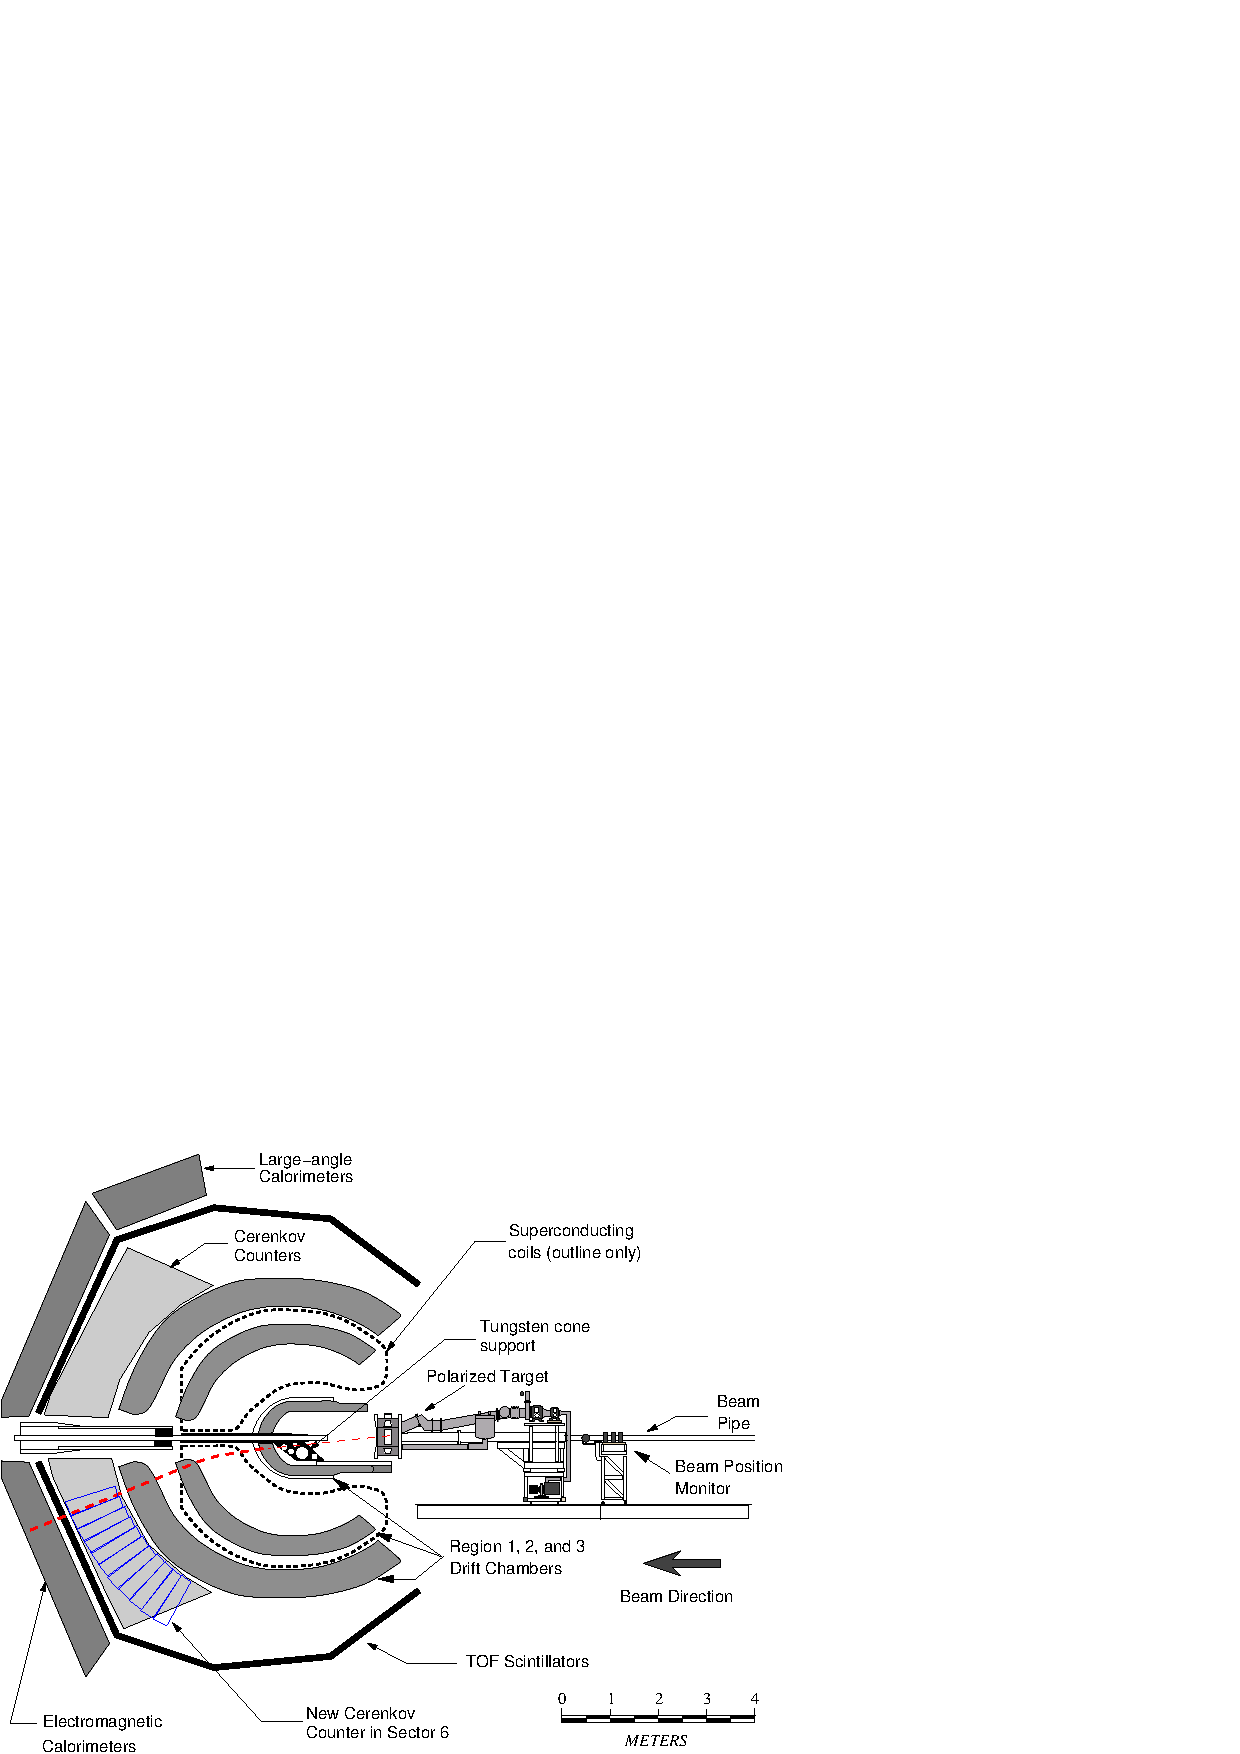
\includegraphics[width=1.0\textwidth]{figuresEG4/FigExp/EG4inCLAS.pdf}  %0.6 is the fraction of the real image width????
\caption[The EG4 setup]{The schematic diagram of the EG4 experimental setup showing the CLAS detector, polarized target system and some beam line elements. }
\label{EG4inCLAS}%{figccunit}
\end{figure}

Other than that the CLAS detector in the EG4 setup (see Fig. \ref{EG4inCLAS}) was used in the standard configuration like in any other polarized target experiments using CLAS. The following list summarizes various specifications of the experimental setup (for more details see \cite{anaNoteXZheng}):
\begin{itemize}
\item \textbf{Beam energies:} 1.3 and 2.0 GeVs for ND$_3$ target runs and 1.0, 1.3, 2.0, 2.3 and 3.0 GeVs for NH$_3$ target runs.
\begin{itemize}
\item \textbf{Beam polarization: } Longitudinally polarized ($\approx 85\%$) electron beam from CEBAF accelerator. Moeller scattering used for the polarization measurement.
\end{itemize}
\item \textbf{Polarized targets: } Solid ND$_3$, and NH$_3$ targets polarized using the technique of Dynamic Nuclear Polarization (DNP).
\begin{itemize}
\item \textbf{Average polarizations: } Between (75 - 90)$\%$ and  (30 - 45)$\%$ respectively.
\item \textbf{Lengths: } 1cm for ND$_3$ and 1 cm and 0.5 cm for  NH$_3$.
\item \textbf{Densities: } 1.056 and 0.917 respectively.
%Packing fraction from Sarah's wiki page: https://clasweb.jlab.org/rungroups/eg4/wiki/index.php/October_28,_2011
\item \textbf{Packing fractions: } (0.624, 0.764) for (1.3, 2.0) GeV  ND$_3$ runs respectively and (0.625, 0.624/0.717\footnote{The two numbers 0.624/0.717 for the 1.3 GeV NH$_3$ runs are due to the fact that two different NH$_3$ targets were used in case of 1.3 GeV runs. One target was in the top cell and the other was in the bottom cell of the target stick.}, 0.716, 0.682, 0782) for (1.0, 1.3/1.3, 2.0, 2.3, 3.0) GeV NH$_3$ runs.  
\end{itemize}  
\item \textbf{Other targets: } Carbon-12 (1 cm and 0.5 cm long), Empty target cup, Target cup filled only with liquid helium (LHe), LHe bath and various foils due to different target chamber windows. 
\item \textbf{Torus currents: } 1500 Amps for 1.0 and 1.3 GeV runs and 2250 A for 2.0, 2.3, and 3.0 GeV runs.
\end{itemize}  
%\subsection{Cherenkov Counters (CC)}

\begin{comment}

\begin{figure}[hp]
\centering
\subfigure[Standard CC module]{% other than $6^{th}$ sector]{
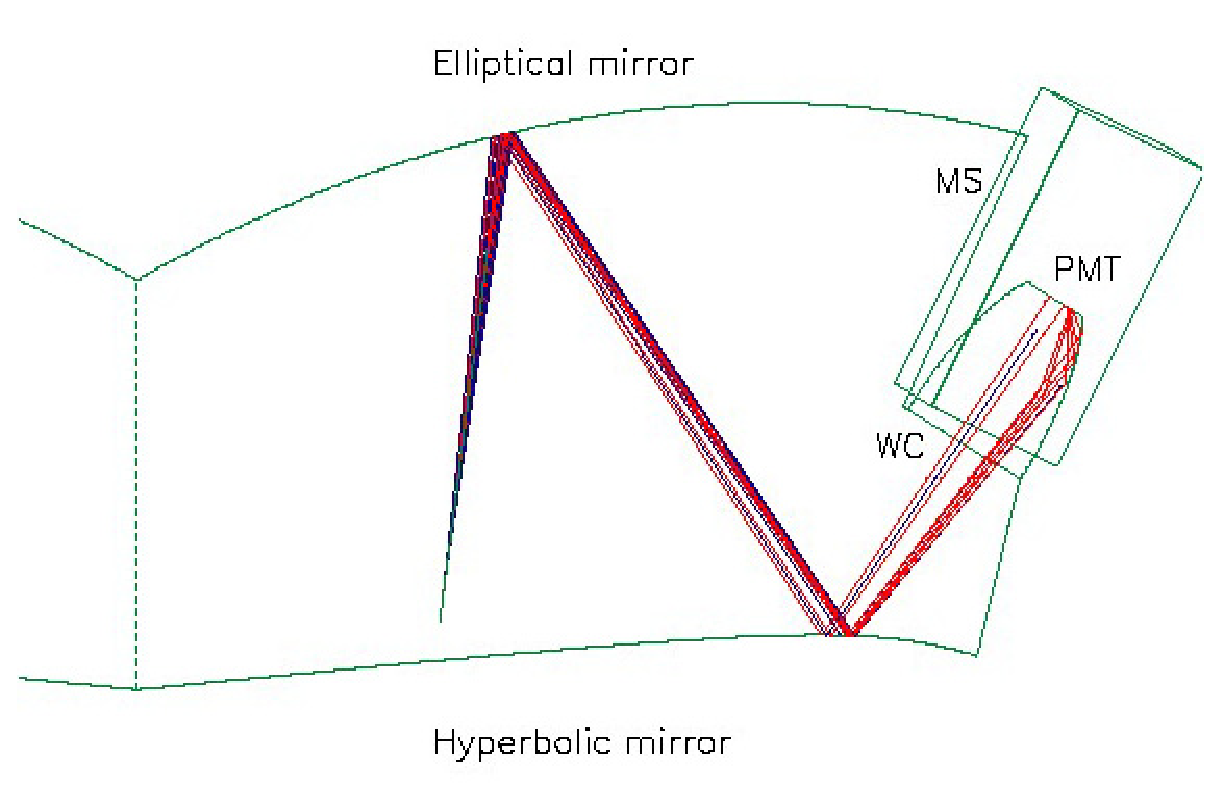
\includegraphics[scale=0.25]{chap6expSetup/Figures/ccmodule.eps}
\label{figccmodule}
}
\subfigure[A CC segment of the standard CC]{
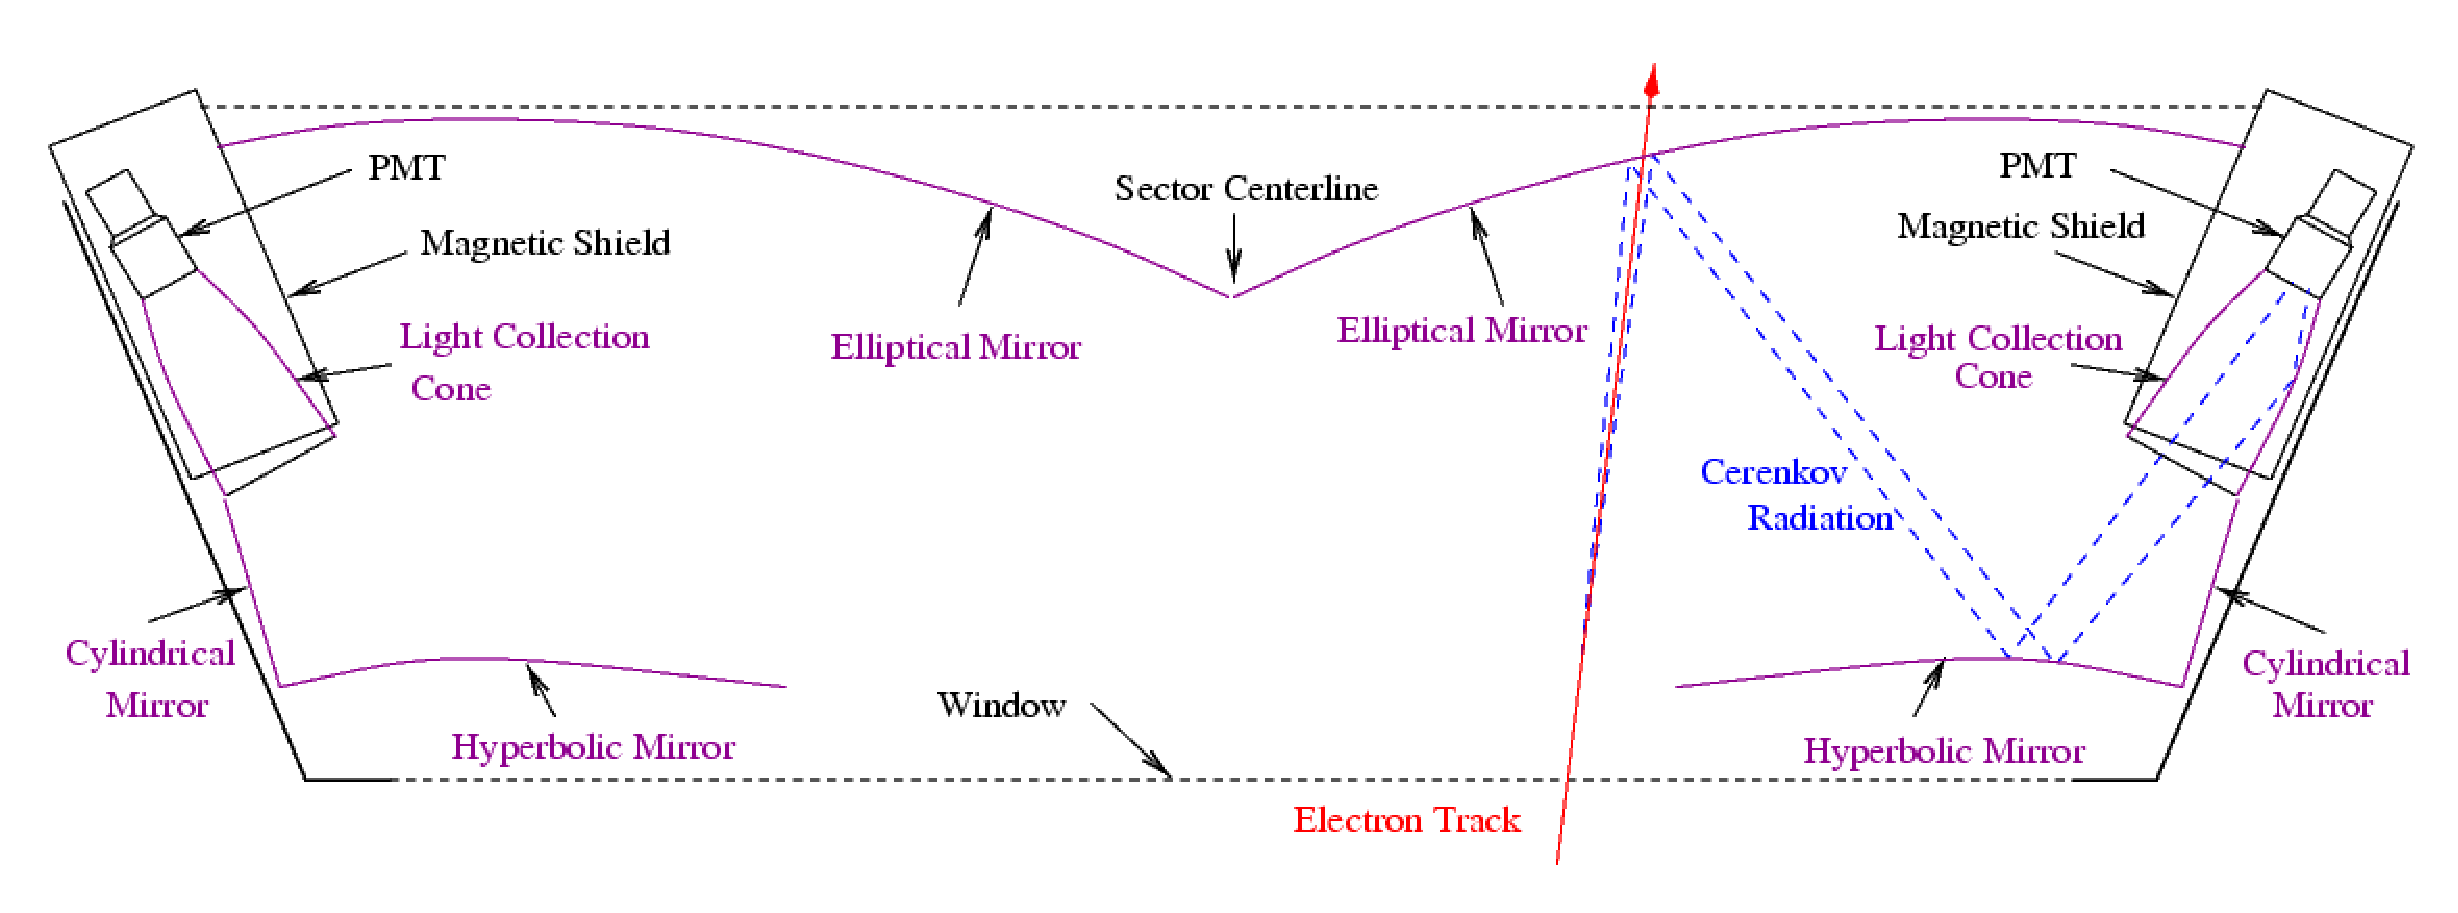
\includegraphics[scale=0.22]{chap6expSetup/Figures/ccsegment.eps}
\label{figccsegment}
}
\label{figcherenkov} %Effect of Dc-smear
\caption[A Cherenkov Counter module]{A Cherenkov Counter (CC) module in CLAS.}
\end{figure}

\end{comment}




\begin{figure}[h] %ht, htpb (p - float, b = bottom, h=? t = top)
\centering
%\leavevmode 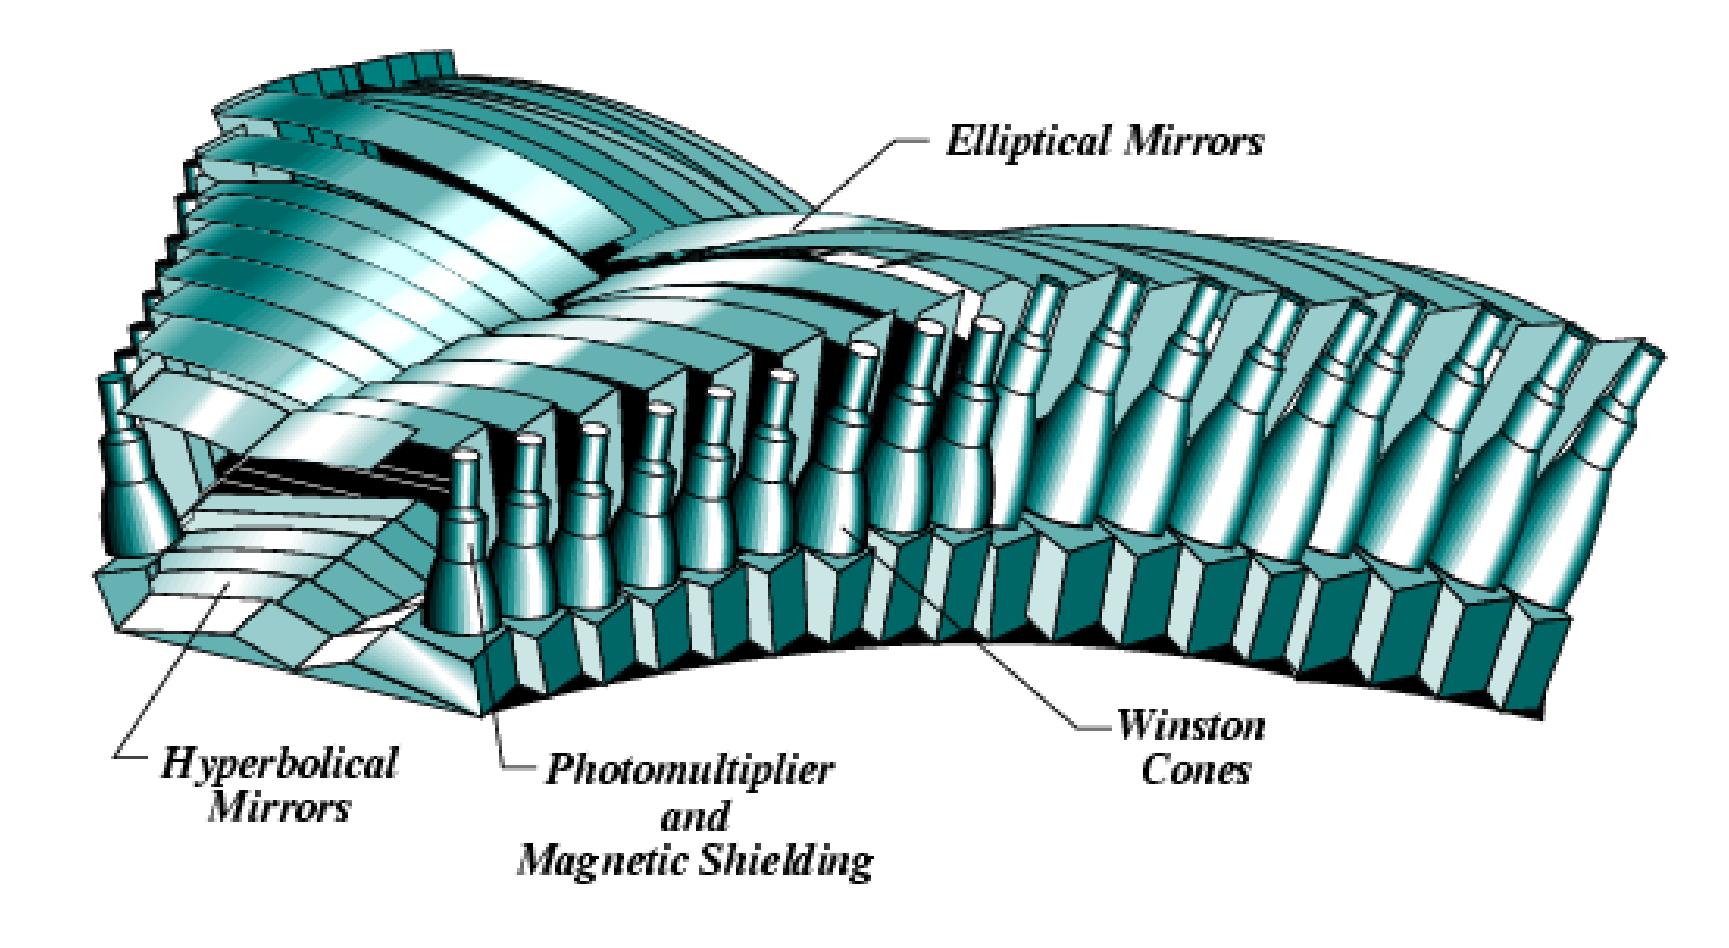
\includegraphics[width=0.8\textwidth]{chap6expSetup/Figures/ccunit.eps}  %0.6 is the fraction of the real image width????
\leavevmode 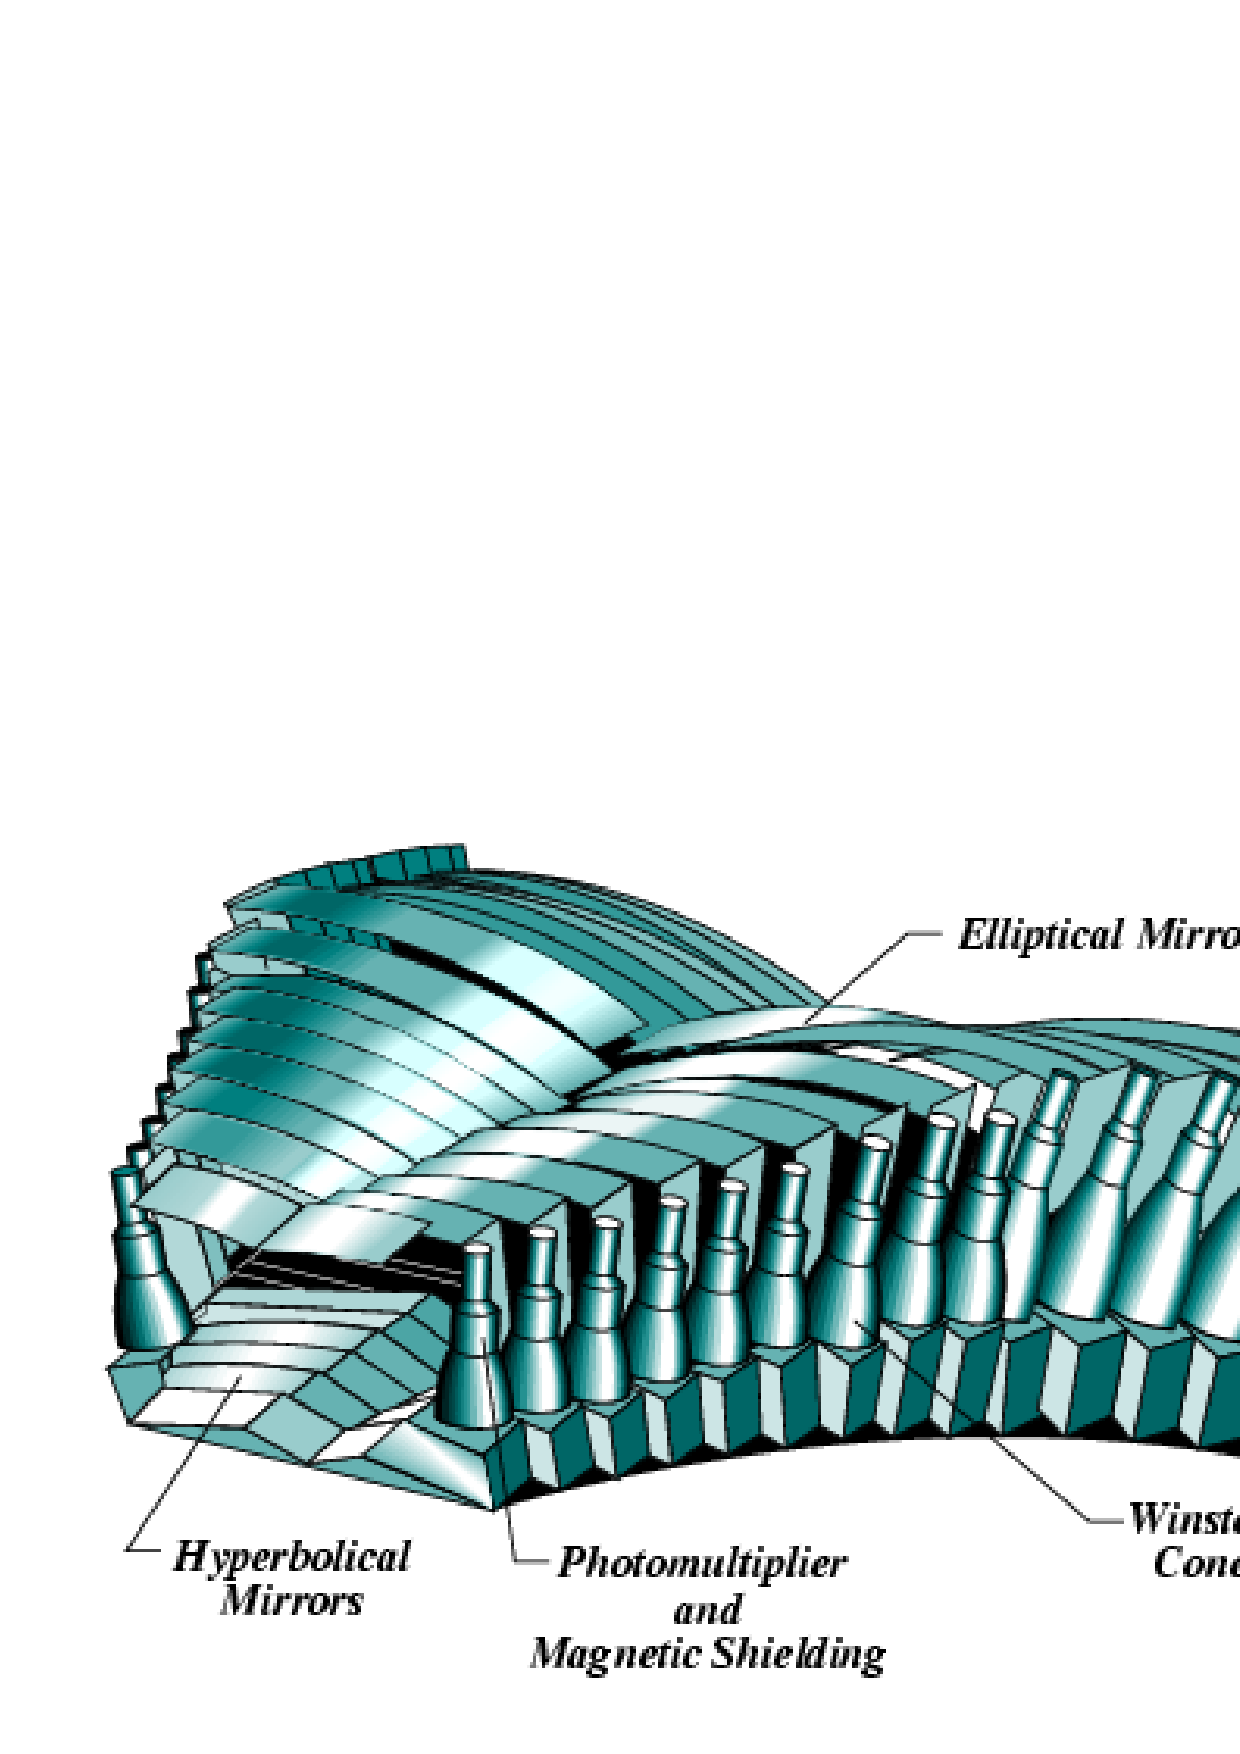
\includegraphics[width=1.0\textwidth]{figuresEG4/FigExp/ccunit.png}  %0.6 is the fraction of the real image width????
\caption[The Standard CLAS Cherenkov Counter]{The computer rendered image of the Standard CLAS Cherenkov Counter}
\label{figcherenkov}%{figccunit}
\end{figure}

\begin{comment}
%\pagebreak   %12/6/13 (because nothing else that I tried worked)

%Threshold Counter https://en.wikipedia.org/wiki/Cherenkov_radiation#Particle_physics_experiments 
The Cherenkov Counters (CC) serve the dual function of triggering on electrons and separating electrons from pions (or identifying charged particles). These detectors use the light emitted by Cherenkov radiation (emission of light when the charged particle travels faster than light in that medium) to measure the particle velocity (and, therefore, $\beta=v/c$). The knowledge of $\beta$ combined with the particle momentum (from the tracking detectors) determines the particle's mass, thus giving us information on %the clue for %SEK
the particle identification. %ID. %GED
%Choosing different gases to fill in, the %GED
The index of refraction (n) is carefully optimized for the particle masses and momentum range of the experiments in question. Threshold counters record all light produced, thus providing a signal whenever $\beta$ is above the threshold $\beta_t$ = 1/n. In the standard configuration, CLAS uses one Cherenkov threshold detector in each of the six sectors in the forward region from $8^o$ to $45^o$.


\end{comment}
\begin{figure}[h] %ht, htpb (p - float, b = bottom, h=? t = top)
\centering
\leavevmode 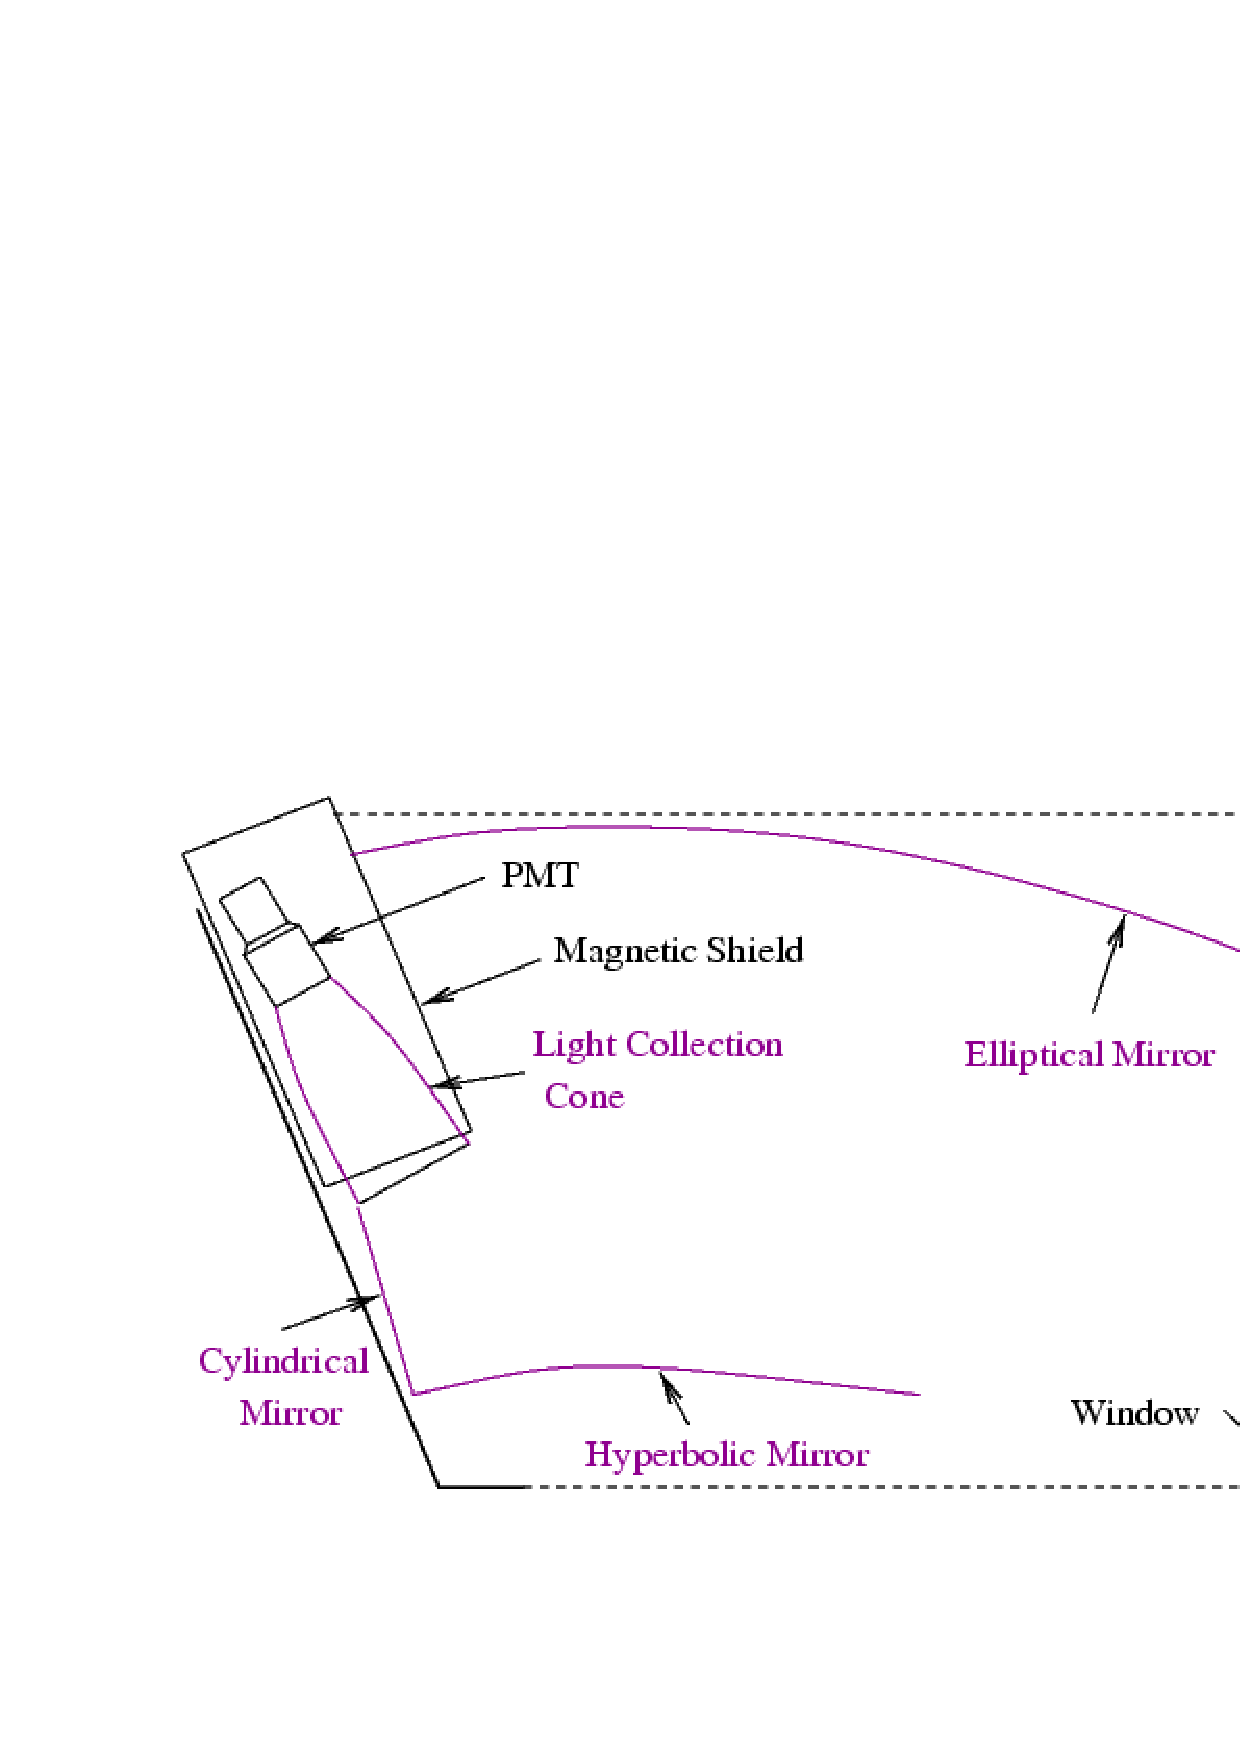
\includegraphics[width=1.0\textwidth]{figuresEG4/FigExp/ccsegment.png}  %0.6 is the fraction of the real image width????
\caption[A Cherenkov Counter module]{The schematic diagram of a CLAS Cherenkov Counter (CC) module showing mirrors, PMTs and the light reflections. %\textcolor{red}{Changed}
}
\label{figccunit}%{figcherenkov}
\end{figure}







%\subsubsection{New CC in the $6^{th}$ Sector}
\section{New CC in the $6^{th}$ Sector}
\label{newCCsec}
%Threshold Counter https://en.wikipedia.org/wiki/Cherenkov_radiation#Particle_physics_experiments 
The Cherenkov Counters (CC) serve the dual function of triggering on electrons and separating electrons from pions (or identifying charged particles). These detectors use the light emitted by Cherenkov radiation (emission of light when the charged particle travels faster than light in that medium) to measure the particle velocity (or rather $\beta=v/c$). The knowledge of $\beta$ combined with the particle momentum (from the tracking detectors) determines the particle's mass, thus giving us information on %the clue for %SEK
the particle identification. %ID. %GED
%Choosing different gases to fill in, the %GED
The index of refraction (n) is carefully optimized for the particle masses and momentum range of the experiments in question. Threshold counters record all light produced, thus providing a signal whenever $\beta$ is above the threshold $\beta_t$ = 1/n. In the standard configuration, CLAS uses one Cherenkov threshold detector in each of the six sectors in the forward region from $8^o$ to $45^o$.



\begin{comment} %Partly redundant with \footnote and also too verbose as per SEK
The standard CLAS Cherenkov detectors (as shown by Figs. \ref{figcherenkov} and \ref{figccunit}) were designed such that their optics, geometry, module position and mirror orientation were optimized for low rate high \qsq experiments that mostly use(d) electron in-bending torus fields. The design was a compromise between the desired kinematic coverage and the complexities of the CLAS detector system including the effect of the torus field. As a consequence, light collection is constrained causing the number of photoelectrons to be strongly dependent on scattering angles, and making the detection efficiency non-uniform, and strongly reduced in some regions (for example, up to 30\% drop in the middle of the sector and at forward angles) \cite{propE03_006}. While it would still be possible to detect electrons, the use of the existing CC would mean that the absolute cross-section measurement would require large and complex corrections which are difficult to evaluate. %be evaluated. In addition, that %SEK
That would significantly contribute to the systematic uncertainties, thus not meeting the proposed high accuracy requirement of the measurements.
\end{comment}

\begin{figure}[h] %ht, htpb (p - float, b = bottom, h=? t = top)
\centering
%Cut out of the designers CAD rendering of the new CC detector http://www.jlab.org/Hall-B/secure/eg4/ripani/Reference/assieme_totale.jpg
%\leavevmode 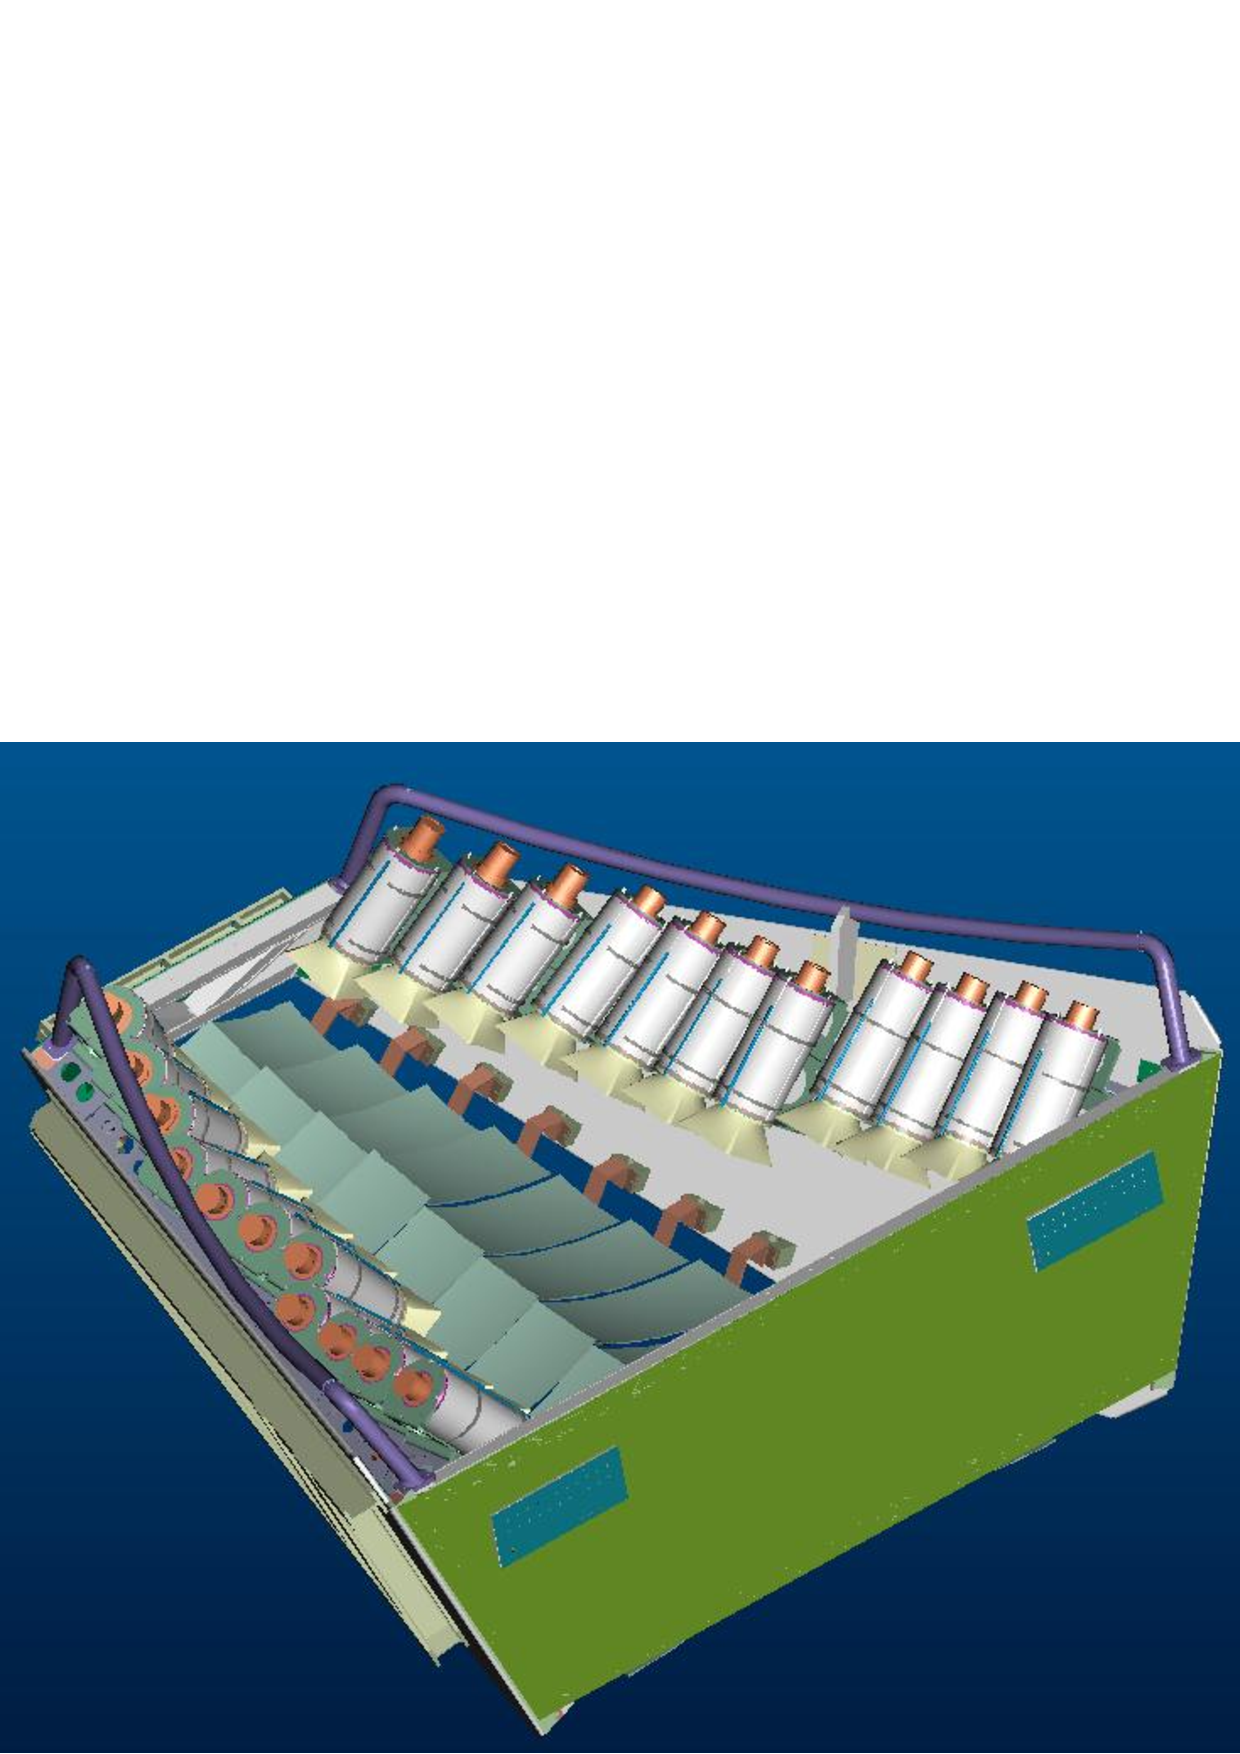
\includegraphics[width=0.8\textwidth]{figuresEG4/FigExp/assieme_totaleCut.pdf}  %0.6 is the fraction of the real image width????
\leavevmode 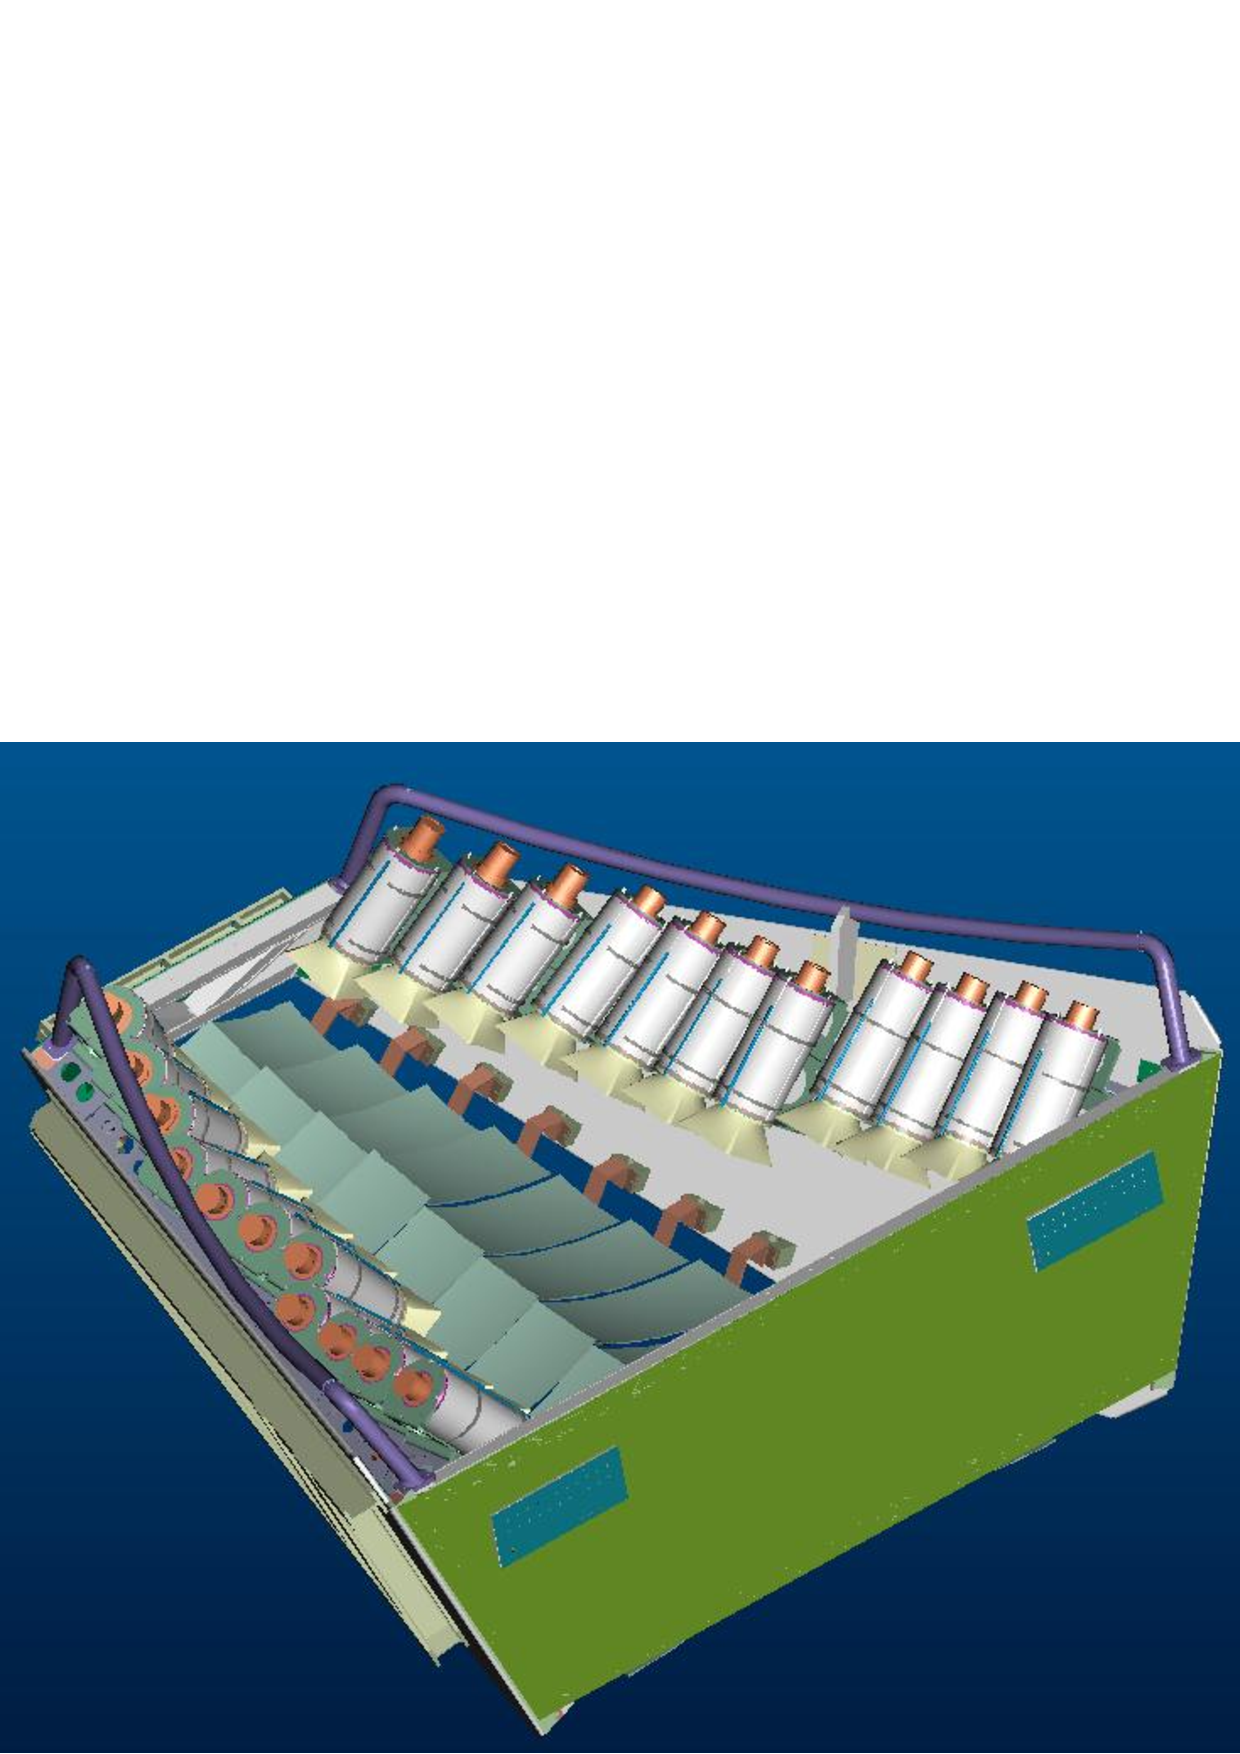
\includegraphics[width=0.6\textwidth]{figuresEG4/FigExp/assieme_totaleCut.pdf}  %0.6 is the fraction of the real image width????
%\leavevmode \includegraphics[width=0.8\textwidth]{figuresEG4/FigExp/assieme_totale.pdf}  %0.6 is the fraction of the real image width????
%\includegraphics[trim={5cm 0 0 0},clip]{example-image-a}  %http://tex.stackexchange.com/questions/57418/crop-an-inserted-image
\caption[New Cherenkov counter]{The new Cherenkov counter (courtesy of INFN, Genova)}
\label{nwCcCAD}
\end{figure}



%In order to avoid having all those CC-related issues in the new measurements, a
A new gas threshold cherenkov counter (designed and built by INFN - Genova, Italy) was installed in the sixth sector. %, with no further modifications of the CLAS. 
This new CC detector (see Fig. \ref{nwCcCAD} for its CAD rendition) is specifically optimized for the out-bending field configuration, which is necessary to reach the desired low momentum transfer (measurements down to 6 degrees). The detector uses the same radiator gas ($C_4 F_{10}$ - perfluorobutane) and the same gas flow control system as the standard %old
one, but it uses a %completely %SEK
different design. %, including mirror types and orientation for light reflection and 
In the new CC, the number of CC-modules %/units 
is now 11 instead of the 18 in the standard ones. In order to maximize the light collection, a single reflection design (see Fig. \ref{newCCphRefl}) using spherical mirrors is used (the standard CC used double relections from elliptical and hyperbolic mirrors). The geometry, the size, the mirror size, position, and orientation, the dimensions as well as the assembly of the modules were optimized for the experiment %using a dedicated FORTRAN code 
and the performance study was %also 
done using a complete GEANT simulation \cite{propE03_006}. Additionally, for the purpose of efficiency and performance studies (see Sec. \ref{secCCineff}), a few special trigger data runs were taken during the experiment. These special runs had the trigger that mainly involved EC-signals (and no CC-signal at all) to decide whether the detected particle was a good scattered electron candidate.


\begin{figure}[h]
\centering
\subfigure[Schematic of a new CC segment.]{
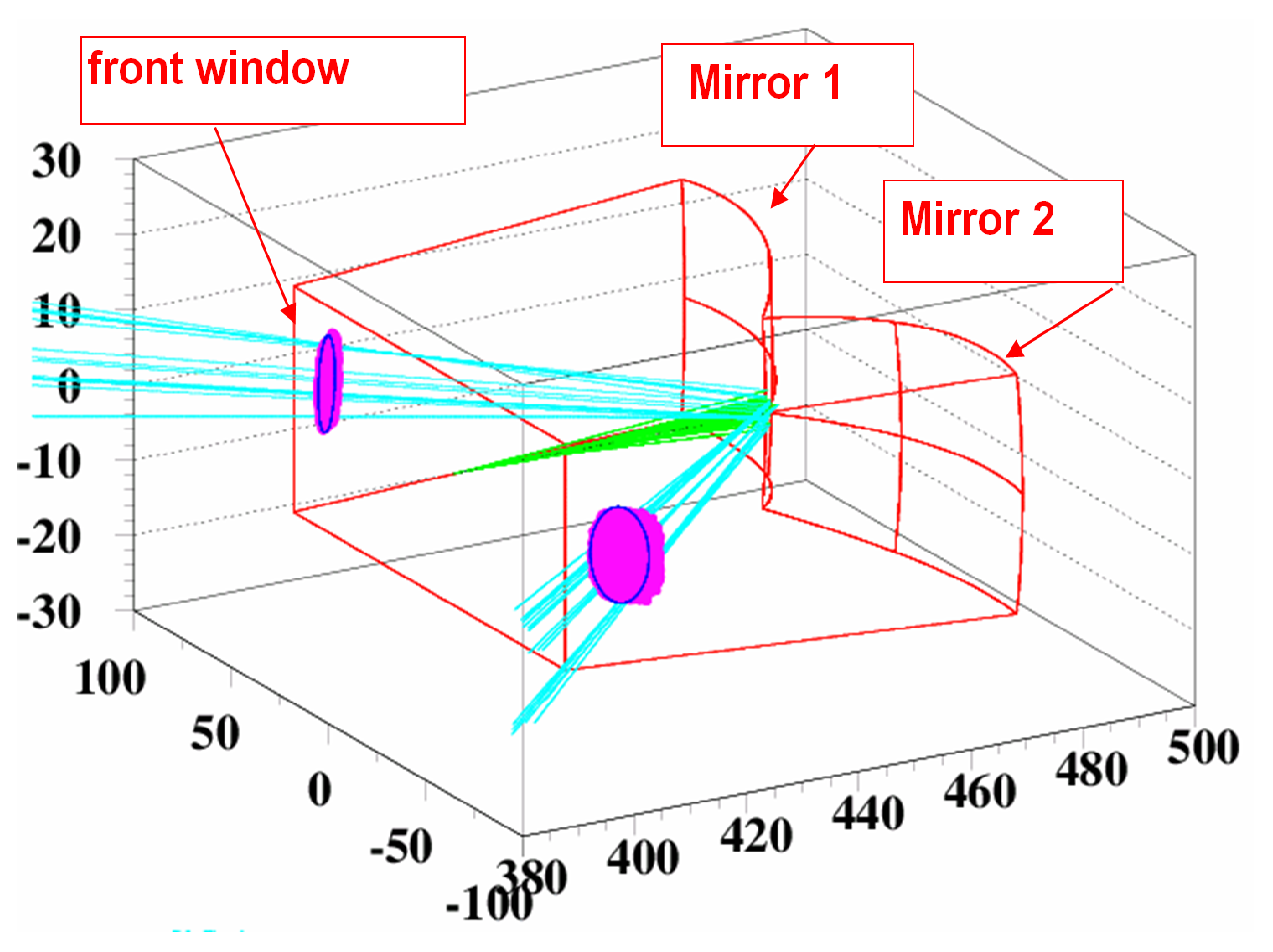
\includegraphics[scale=0.32]{figuresEG4/FigExp/newCCmoduleLights}
\label{nwCCunit}
}
\subfigure[Schematic of light reflections.]{
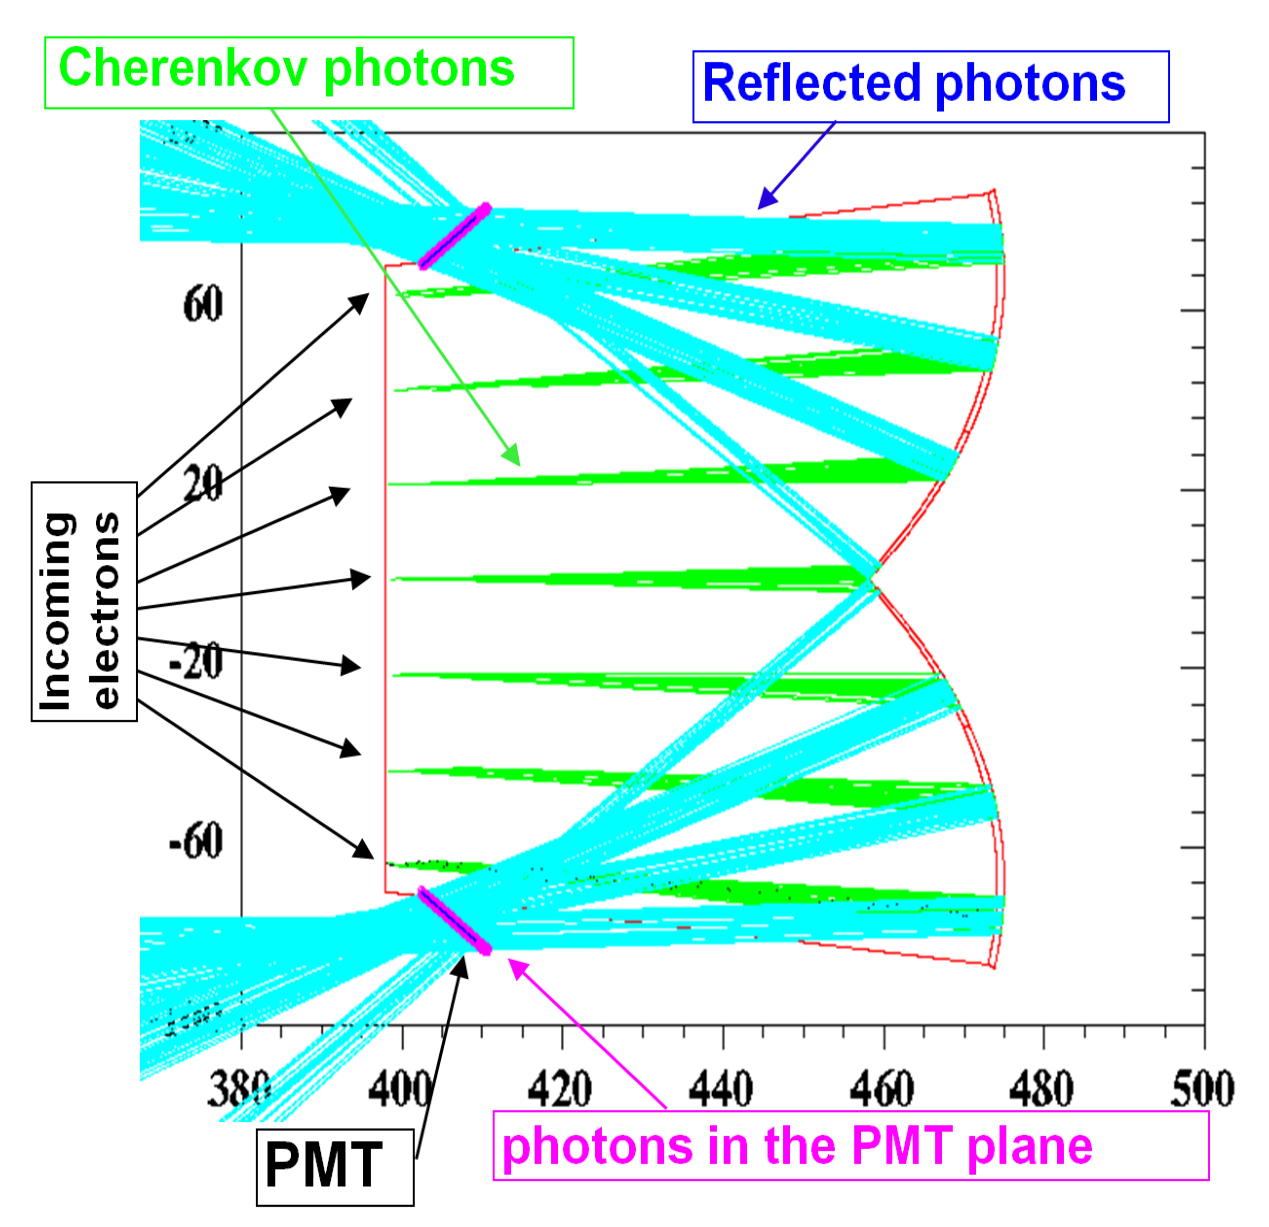
\includegraphics[scale=0.28]{figuresEG4/FigExp/cerenkovLightReflection}
\label{newCCphRefl}
}
\caption[A new CC segment and light reflections]{Schematic of a new CC segment showing the arrangements of the mirrors, PMTs and the light reflections (courtesy of INFN, Genova).}
\label{figcherenkovNw} %Effect of Dc-smear
\end{figure}


%This new detector achieves a very high and uniform electron detection efficiency ($\approx$ 99.9\%) in most of its central (fiducial) region, to allow for the measurement of the absolute cross-section with minimal corrections and a high pion rejection ratio (of the order of $10^{-3}$). Due to the high electron rate at low \qsq, the \ph coverage can be lowered, while still having a large counting rate. %, we will have an overwhelmingly large amount of scattering at smaller angles, 
%Therefore, for reasons of limited data storage capability, and also for the fact that only the sixth sector had the required new CC, only the sixth sector events were collected, stored and subsequently used for data analysis.% \cite{jlabVocab_wb}.





\clearpage
%
%\chapter{Electron Identification}
\chapter{Data Analysis Procedure}
\label{dataAnal}

The goal of this data analysis is to extract the spin structure function $g_1$ for the deuteron and evaluate its moments. Since the product $A_1F_1$, which is proportional to $\sigma_{TT}$, directly enters sum rules for the real photon point, which leads to the generalized GDH integral ($\bar{I}_{TT}$) and the generalized forward spin polarizability ($\gamma_0$) being expressed in terms of the first and third moments of the product $A_1F_1$, we decided also to extract the product $A_1F_1$ using exactly the same procedure as for \gone. 

The extraction of both \gones and \afones depend directly on the measurement of the following polarized cross-section difference:

\begin{equation}
  \Delta \sigma_{\parallel} = \frac{d^2\sigma^{\downarrow \Uparrow } }{d\Omega dE'} - \frac{d^2\sigma^{\uparrow \Uparrow } }{d\Omega dE'}
  %= \frac{1}{N_t}\cdot \left[ \frac{N^+}{N^+_{e^-}} - \frac{N^-}{N^-_{e^-}} \right]\cdot \frac{1}{P_bP_t} \cdot \frac{1}{\Delta\Omega}\cdot \frac{1}{E_{detector}}
    = \frac{1}{N_t}\cdot \left[ \frac{N^+}{N^+_{e^-}} - \frac{N^-}{N^-_{e^-}} \right]\cdot \frac{1}{P_bP_t} \cdot \frac{1}{\Delta\Omega}\cdot \frac{1}{\eta_{detector}}
  \label{eqXSdiff}
\end{equation}

where, 
\begin{itemize}
  \item $N_t$ = Number density of deuteron nuclei in the target 
  
\begin{comment}  
  \item $N_t$ = Number of deuteron nuclei in the target = $3 N_a l_A \frac{\rho_A}{m_A}$, with 
    \begin{itemize}
      \item 3: number of Deuteron atoms in a \hnd3 molecule
      \item $N_a = 6.02\times 10^{23}$: Avogadro's number
      \item $l_A =$ target length (cm) $\times$ packing fraction
     % \item $\rho_A = 0.917 (g/cm^3)$: Target density
      \item $\rho_A = 1.056 (g/cm^3)$: Target density
            %\item $m_A = 18.023584 (g)$: Mass of target molecule \15nd3  
      %\item $m_A = 20.0474 (g)$: Mass of target molecule \lnd3  
      \item $m_A = 21.042414237 (g)$: Mass of target molecule \hnd3   %Calculated myself by using the masses of 15N and deuterons
      %I spent a whole day trying to find the 15ND3 mass by googling, but to no avail. So, above value is a temporary solution.
      % Molecular Weight of 15NH3: 18.0239 g/mol   http://www.chembase.com/cbid_107639.htm
      % Molar mass of ND3 is 20.0474 g/mol;  http://www.webqc.org/molecular-weight-of-ND3.html (it's 14ND3)
      % 14ND3 = 14.0030740048+3*2.01410178 = 20.04537934 (Calculated myself)
    \end{itemize}
\end{comment}
    
  \item $N^{+/-}$: Number of scattered electrons (off deuteron only) for each helicity state (+/-).
  \item $N^{+/-}_{e^-}$: Number of incident electrons for +/- helicity states 
  
\begin{comment}    
  \item $N^{+/-}_{e^-}$: Number of incident electrons for +/- helicity states = $\left(\frac{ C_{Fcup}^{+/-}\cdot (10^{-9}/9264)}{Q_{e^-}} \right)\cdot \frac{C_{BPM}}{C_{Fcup}}$ with 
    \begin{itemize}
      \item $C_{Fcup}^{+/-}$: Helicity dependent Faraday-cup counts (live time gated)
      \item $\frac{10^9}{9264}$: Factor for converting Faraday cup counts into coulombs. (The factor 1/9264 converts the counts into nano-coulombs.)
      \item $Q_e = 1.0602\times 10^{-19}(C)$: the electron charge. %kp: electronic charge.
      \item $\frac{C_{BPM}}{C_{Fcup}}$: the ratio of the Beam-Position-Monitor (BPM) and Faraday-cup counts. The BPM is located before the target so its count doesn't suffer the loss, but the Faraday-cup is located at the end of the beamline and because its physical radius is not large enough, parts of the beam's halo are not collected. Since, the size of the halo depends on the amount of material in the beamline as well as on the beam energy, the ratio is a function of the beam energy. For high beam energies such as 3 GeV, the ratio is close to 1 but for the lower beam energies it is lower than 1. For example the ratio is 0.965919 for 2.3 GeV\cite{HK_dXs_extr}. 
    \end{itemize}
\end{comment} 
   \item $P_bP_t$ = Product of the beam and target polarizations
   \item $\Delta\Omega=\sin\theta\cdot\Delta\theta\cdot\Delta\phi$: The solid angle for the given kinematic bin. %, also commonly known as ``detector acceptance''. %\textcolor{red}{Am I right about ``Acceptance''?}
   This term includes the ``detector acceptance''.
%   \item $E_{detector}$ %stands/
   \item $\eta_{detector}$ %stands/
   accounts for the detector efficiencies
 % \item The third etc \ldots
\end{itemize}

The data analysis to extract the physics quantities involves accurately measuring each of these quantities, either separately or in some combined form. To do so, the data must be properly reconstructed, calibrated and corrected to build all the scattering events during the experiment. Since the reconstructed events include a wide range of physical processes in addition to the electron-deuteron scattering process that we are interested in, proper event selection cuts must be applied. In this chapter, all these steps from the data reconstruction and calibration through the extraction of \gones are described.

%\begin{comment} 
%This is the first/leading file on the whole ``Data_Analysis Chapter
%Created by kp on Sep 8, 2013

\hspace{0.5cm}

\section{Raw Data Processing - Calibration and Reconstruction}   %Calibration and Reconstruction?
\begin{comment}
The raw data recorded by the CLAS DAQ system consist of ADC and TDC values registered by different components of the detector (in response to the passing of various particles through them) and also some beam related information such as Faraday Cup readings and beam helicity information. These data are collected and saved (by the DAQ system) in the fortran-77 based BOS format \cite{bos} which implements a dynamic memory management. %citation needed here (De Vita tesi, 51/65)
In the BOS file, the data is organized into banks, with each bank carrying data belonging to a particular detector or some part of it. Each bank consists of two parts - header and body. The body contains the actual collected data (such as the ADC and TDC values from detector components such as PMTs, in the case of raw data, or information such as energy and time in case of the reconstructed data), while %but 
the header contains some relational information - such as the bank identifier, the number of rows and columns of data in the bank and the location of the next bank. In the case of reconstructed data, in addition to the banks carrying detector specific reconstructed information such as the energy and time of the signals, more banks are added to the data file for storing high level information such as the number of particles detected in a given event, the four-momenta of each of the particles etc. 
\end{comment}

The raw data recorded by the CLAS DAQ system, which consists of ADC and TDC values registered by various detector components as well as the beam related information such as beam helicity and Faraday Cup readings, are organized into banks (with each bank carrying data belonging to a particular detector component or some part of it) and saved in special format (BOS) files. These raw data are next processed with a standard CLAS software package called RECSIS, which analyzes and combines the matching bits and pieces of the raw information to reconstruct particles and events that produced them. Such reconstruction produces output data that consist of event and particle IDs, particle positions and energies and momenta (in the lab frame CLAS coordinate system), and also some static particle properties such as charge and mass. The reconstruction program uses geometric parameters and calibration constants (from the %available 
CLAS Calibration Database) for the detector %(determined separately) 
in order to properly process and transform the raw data into the reconstructed tracks.


The first part of the data processing is the detector calibration. In this phase, a small sample (about 10\%) of raw data (uniformly selected over the entire run period to ensure time stability verification) is chosen and the energy and time calibration constants are adjusted to give the correct behavior while constantly monitoring related variables. This is done separately for each run period to consider the different running conditions, the possibility of unwanted changes in hardware that may have occurred, as well as drift of detector response over time. This process of adjusting the calibration constants and reconstructing the data is repeated until a desired level of accuracy is reached. Once that level is reached, the calibration constants are ``frozen'' and the final reconstruction is done. The resulting output is saved in especial formats\footnote{Two especial data formats - BOS and ntuple (h10) - were used}.
These saved data provided the starting point for our higher level data analysis as described in this dissertation. %The details of the calibration and reconstruction process can be found in \cite{rdVita_th}.

The iterative work of data reconstruction and detector calibration, which was a very computing intensive and time consuming, was done by R. De Vita - one of the EG4 collaborators from  INFN, Genova, with good expertise on CLAS data reconstruction - soon after the data collection was completed (from 2006-2007). The data from this ``Pass1'' reconstruction was first analyzed as part of the Ph. D. dissertations by three graduate students, but during these analyses, a few anomalies\footnote{The anomalies observed in the pass1 analysis were the discretized reconstruction of vertex and wrong reconstruction of track positions in DC1.} in reconstruction were observed which were later tracked down to a %https://clasweb.jlab.org/rungroups/eg4/wiki/index.php/User:Lamiaa#EG4_Software_Update_.26_Solution
mixing up of codes from two EG4 sub-packages for the reconstruction software. After the mix-up was sorted out, a new pass (Pass2) of reconstruction was performed by L. El Fassi (still using the same calibration constants as used by the Pass1 reconstruction). The data from this latest pass of reconstruction was used for the analysis reported in this note 


\section{Helicity States}

%\textcolor{red}{More to be done.}
\begin{figure}[H]%[h] %ht, htpb (p - float, b = bottom, h=? t = top)
  \centering
  \leavevmode 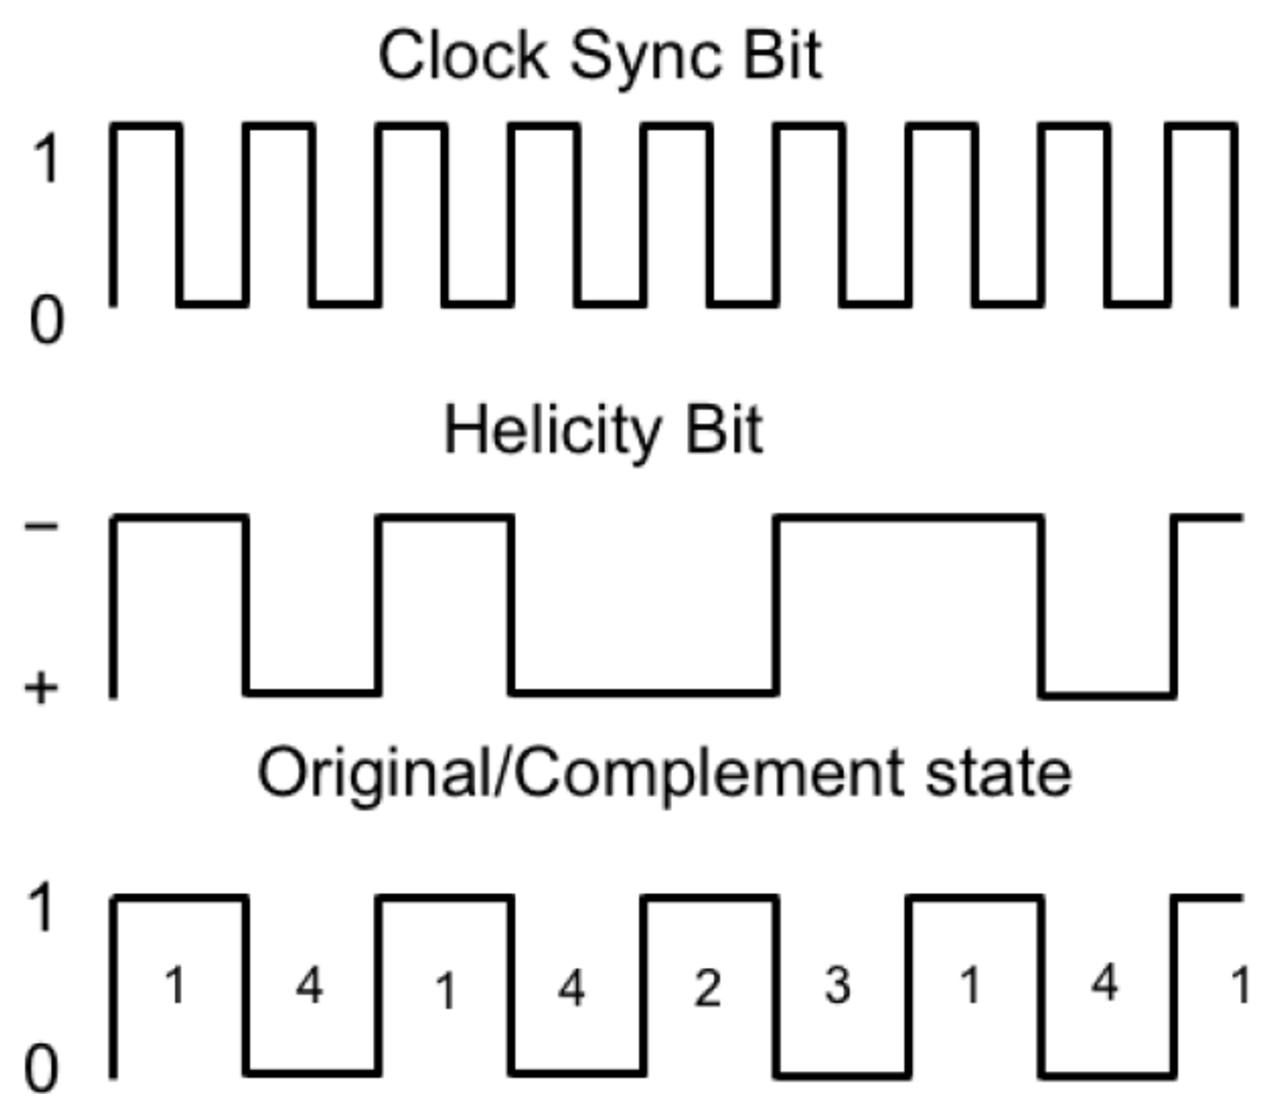
\includegraphics[width=0.4\textwidth]{figuresEG4/FigSim/helicityPairingNevzatCut} 
  \caption[Helicity Pairing]{Different data signals sent from the injector that monitor the helicity states of beam electrons. (Fig. courtesy of N. Guler \cite{nGuler_th} ).}
  \label{figHeli}
\end{figure}
%Prok pg 138, https://clasweb.jlab.org/rungroups/eg4/wiki/index.php/User:Devita; Sulkosky pg 70

As we saw from Eq. \ref{eqXSdiff}, the physics %quantity 
extraction depends on %the
measurements of the number of events in %counts for 
the two (+/-) electron helicity states. The CEBAF accelerator provides the polarized electrons in closely and % but 
equally spaced bunches. These bunches are further grouped into ``buckets'' according to their helicity states, which are %is 
alternated pseudo-randomly at the injector with a frequency of 30 Hz. The information on the helicity state of each of the buckets and the total integrated charge contained in it is injected into the DAQ data stream immediately after the helicity flip. Using a combination of different types of sequence control signals sent from the injector (see Fig. \ref{figHeli}), it is possible to determine which helicity state a particular event belonged to, which then can be used to label the helicity state of the event in the data stream, %its 'HEAD' bank, 
together with the total beam charge of the state.


\begin{comment}
This is called the original state. The original state is always followed by a complement state. The information about the helicity state and the total integrated charge for that helicity state are stored in the data stream after each helicity flip (sometimes the information was injected after 2 helicity flips depending on the DAQ throughput). A sync pulse, with twice the frequency of the helicity pulse, is also delivered to the experimental hall and stored in the data stream. The sync pulse is used to identify the helicity flips and detect missing helicity bits. The original helicity state is always labeled with 1 or 2, while the complement state is labeled with 3 or 4. The original helicity pulse labeled with 1 should always be followed by a complement helicity pulse labeled with 4. Similarly, 2 should always be followed by 3. The flip should always coincide with the rising edge of every other sync pulse. Fig. \ref{figHeli} shows the flow of helicity states together with corresponding helicity bits labeled with + or − . Knowing the order of helicity labels, one can identify if any helicity state was missed due to dead time problems in the DAQ system. A broken sequence leads to unpaired helicity states, which would introduce a false asymmetry. It was determined that the helicity label stored in each physics event sometimes failed to latch leading to a broken sequence. Fortunately, the Faraday Cup scaler had its own helicity label latch which did not fail. The information from the FC scalers was used to recover the correct sequence.


An algorithm, as a part of the “HelP.cc” [92] program, was designed to track down the helicity states and determine the problematic helicity buckets. The algorithm was incorporated as a part of the DST library and the necessary flags to identify correct helicity sequencing were written into the DST files. The code extracts the helicity in terms of 1 or 0 or a number less than 0, which indicates that the helicity state is suspect. 5 The negative values are encoded according to the list in Table 6. While processing the DST files for analysis, a program called PATCH was used to produces tables for each DST data file to monitor the helicity sequence and throw
away bad helicity buckets. The tables produced by PATCH include minimum and maximum event numbers for each helicity bucket together with the labels of original or complement states and the corresponding helicity bits determined by the HelP algorithm. The table also includes the minimum and maximum event numbers from scaler BANKS in the DST and finally a flag for the helicity bucket indicating whether it is good (flag = 1) or bad (flag = 10,-1000). The PATCH program labels any helicity state smaller than 1 or larger than 4 with -10. These states will be disregarded from further analysis. The program also examines the order of the helicity states and determines the buckets that are out of sequence. It also compares minimum and maximum event numbers from the trigger banks with the output of the scaler banks and labels unmatched helicity buckets. The label for these two latter cases is - 1000. In addition, PATCH takes care of suspicious helicity states at the end of some DST files that occur during file closing. Whenever a bad helicity bucket is found, the original and the complement states are always thrown away together until the correct sequence is recovered. This ensures that the removal of problematic buckets will not bias any particular helicity state. During the analysis process, the PATCH program is executed first and its output table is used by the DST reader to determine problematic helicity buckets. A segment from its output is shown in Table 7.
\end{comment}




\section{Electron Identification}
\label{allCuts}

In CLAS electron-scattering %(electro-production) %SEK/GED
experiments, the scattered electron defines the timing of each event. In addition, in inclusive measurements, the scattered electron is the only particle 
to be detected and measured. So, it is particularly important to make sure that electrons are well measured and properly identified and are 
not contaminated with misidentified particles such as negative pions (\pim) or lost by being misidentified. %as something else, thus affecting the accurate measurement of cross sections. In particular, \pim and electrons give rather similar detector signals and, therefore, are difficult to discriminate in some kinematic regions.

%%%%%In each event the electron candidate is the negative track that triggered the event. The trigger condition is ensured by choosing the first entry in the event bank and also requiring that the track has hit matches in CC, DC, EC and SC and is also time-based (positive DC status word in DCPB). 
%%% ThCp
%
The process of identifying the primary scattered electrons starts by first rejecting all those particle 
candidates which are not the first entries (i.e., the trigger particles) in the event bank. The 
remaining sample of the candidates is refined further by rejecting those with positive
charges. Then, the sample is further refined %After that they are filtered more 
by applying a set of cuts %selection conditions (commonly known as ``cuts'') 
that are listed and described below. An electron candidate is considered good if it passes %through 
all of these cuts.
%
%%% ThCp
%All four layers of detectors are important in identifying electrons. For example, tracking by DC decides the charge of a candidate, SC records the time of flight, which is important in the time-matching criteria as mentioned below. The following list shows criteria/cuts defining a good electron starting from a candidate electron.
%%% ThCp

\begin{enumerate}
\item {\bf Good Electron Cuts}
\begin{enumerate}
\item {\bf Cut on particle charge:}  q=-1
\item {\bf Detector status cuts:}  
\begin{enumerate}
\item {\bf DC status:}  dc\gt 0; dc\_part\gt 0
\item {\bf SC status:}  sc\gt 0; sc\_part\gt 0 
\item {\bf EC status:}  ec\gt 0; ec\_part\gt 0  
\item {\bf CC status:}  cc\gt 0; cc\_part\gt 0  \\
             (For simulated data, all of the above except those on CC variables are used.) % (see Sec. \ref{}).)
\end{enumerate}
\item {\bf Electromagnetic Calorimeter Cuts}  (see Sec. \ref{ecCuts})
\item {\bf Osipenko cuts} Cuts on CC angle \th, \ph and time matching between CC and other detectors. (see Sec. \ref{osiCuts})
\item {\bf Cut on minimum number of photoelectrons}  (see Sec. \ref{nphCut})
\end{enumerate}
\item {\bf Good Event Cuts}
\begin{enumerate}
\item {\bf Cut on minimum number of particles detected and reconstructed in the event:} gpart\gt 0 
\item {\bf Minimum/maximum momentum cuts} (see Sec. \ref{pCuts}) %p\gt0.2$\times E_{beam}$ and p\gt0.3   %This may be a little out of order here %   $\cdot
\item {\bf Sector cut}  dc\_sect = 6; cc\_sect = 6 (to select electrons from the sector where the low momentum Cherenkov detector was installed)
\item {\bf Scattering vertex-z cuts}  (see Sec. \ref{vzCuts})
%\item {\bf Cut around a hole in $\theta_{DC1}$:}  %(This removed because our new fiducial cuts considers it)
%\item {\bf Vertex theta cut:}                     %(This removed because our new fiducial cuts considers it)
\item {\bf Fiducial cuts}  (see Sec. \ref{fidCuts})
\end{enumerate}
\end{enumerate}

%\textbf{\textcolor{red}{Comment: This section may be moved to another chapter later on .}}\\ %\\%\newline
%It will be seen later that the %SEK
This data analysis relied on comparing the experimental data with a Monte-Carlo simulated data set that was as realistic as practically possible. %The simulation process involves first the simulation of the physics process of inclusive electron scattering, then simulation of the CLAS detector response when the scattered electrons passed through it and finally reconstructing the events from the simulated detector responses using the same reconstruction software as used for the real data. 
Thus, we also have to analyze the simulated data in the same way as the experimental data. % requiring similar event selection cuts of their own. 
In the ideal situation, all cuts would be the same for both %types of 
experimental and simulated data. However, %But, despite our best efforts, 
we could not make our simulation match perfectly with our experimental data.% to the expected level. %- mainly due to some previously unseen issues with the reconstruction software (RECSIS). 
Therefore, some of the data selection cuts are defined separately for the two cases and sometimes separately even for different \qsqs bins (to make sure we have the same fractions of events in corresponding kinematic bins for %on
both type of data).


%\section{EC-Cuts}
\subsection{Electromagnetic Calorimeter Cuts}    %  nwTgtEcCt = NewTgtECcuts(..) in ~/LinkedFiles/evS\subsection{Electromagnetic Calorimeter Cuts}    %  nwTgtEcCt = NewTgtECcuts(..) in ~/LinkedFiles/evSelectionCutsAllinOne.h
\label{ecCuts}

The EC cuts consist of two %three
different cuts applied together. One of these is on the sampling fraction i.e. the fraction of the energy deposited in the calorimeter, and the other is on the energy fraction deposited in the inner part of the calorimeter. % and the last is based on the correlation between the inner and outer energies recorded by the calorimeter.

\begin{comment}
%Inside NewTgtECcuts  we have the following with Q2 dependent values for sfCt (Using same width cut on the left as that for CLAS data
%    to ensure same fraction of data)
bool NewTgtECcuts(int DataOrSim,int Eb_index, float pp, float ei, float eo, float et, float beta, int Q2bin) 
{
  double sfCt=0.2, sfCut=0.2; if(Q2bin<15) sfCut=0.15;
  double sigmaTimes=(MeanSfClas[Q2bin]-sfCut)/SigmaSfClas[Q2bin]; //Distance of sfCut(==0.2 or 0.15 etc) from mean in units of sigma
  if(DataOrSim==1)
    {
      sfCt=sfCut; 
    }
  else if(DataOrSim==0)
    {
      sfCt=MeanSfSim[Q2bin] - SigmaSfSim[Q2bin]*sigmaTimes; //Using the same width cut on the left as that for CLAS data to ensure same fraction of data 
    }
  //See *.gif & *.txt files with name starting with ecCuts_sfOneD_Eb2 & ecCuts_eiOneD_Eb2 in http://wwwold.jlab.org/Hall-B//secure/eg4/adhikari/Analysis/SimStuffs/CutsPlots/ (Sim data made with VzD32, Vz=-100.93 & NewVzCuts(..) above.
  if( et/pp>sfCt    &&    ei>0.06    &&   (eo/pp >= -(0.20/0.11)*ei/pp + 0.20)) return true; else return false;
}
\end{comment}


\subsubsection{Cuts on EC sampling fraction}
%\textbf{\textcolor{red}{Comment: Show plots from one or two Q2 bins and list all other cuts in a table (may go to Appendix)}}
While moving through the EC, charged pions are minimum ionizing particles in the momentum range detectable by CLAS. On the other hand, each electron deposits its total energy $E_{tot}$ in the EC\footnote{Because some of the deposited energy is in the lead part of the EC rather than the scintillator, only a fraction of the electron energy is detected in the EC.} %\footnote{Due to occasional mismatching with momentum information from DC during the reconstruction process, $E_{tot}$ is not always calculated to be the sum of the energies deposited in the inner and outer parts of EC. Therefore, in our analysis, we calculate $E_{in}$ + $E_{out}$ and if this sum turns out to be larger than $E_{tot}$, then we choose the sum as the true value of $E_{tot}$.} 
by %undergoing/
producing electromagnetic showers. %($E_{tot} \approx p$ for electrons that have high energies). %which is proportional to its momentum p. 
Therefore, the sampling fraction $E_{tot}/p$ should be independent of the momentum for electrons (in reality there is a slight dependence). 

\begin{figure}[H] %ht, htpb (p - float, b = bottom, h=? t = top)
%\leavevmode 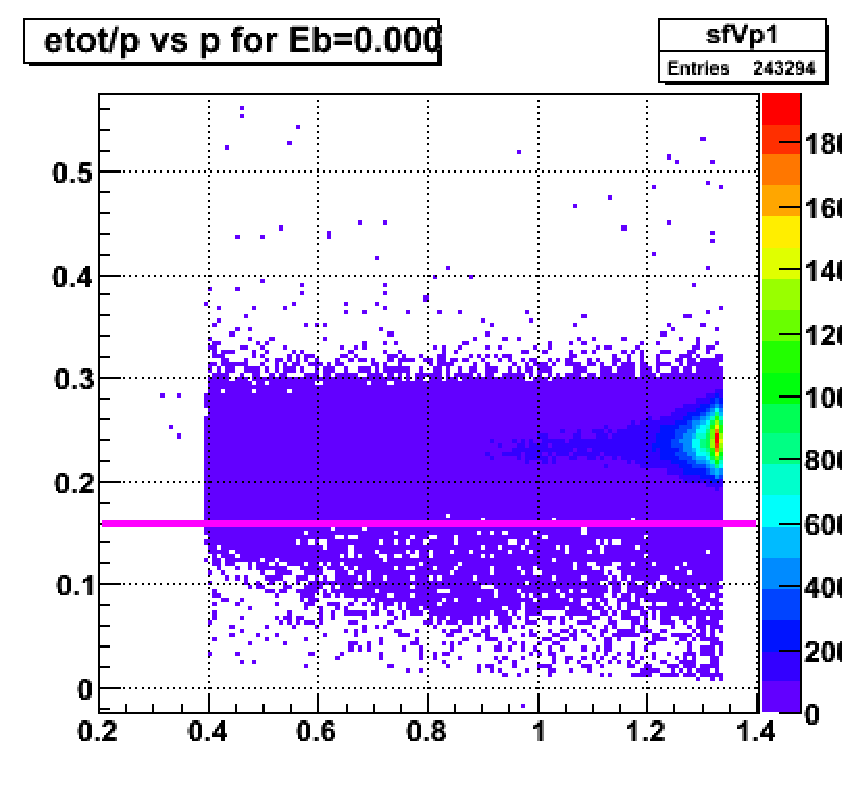
\includegraphics[width=1.0\textwidth]{chap4simul/FigConv/stdECcutsSfvP_Eb1.eps}  %0.6 is the fraction of the real image width????
\centering
%\leavevmode 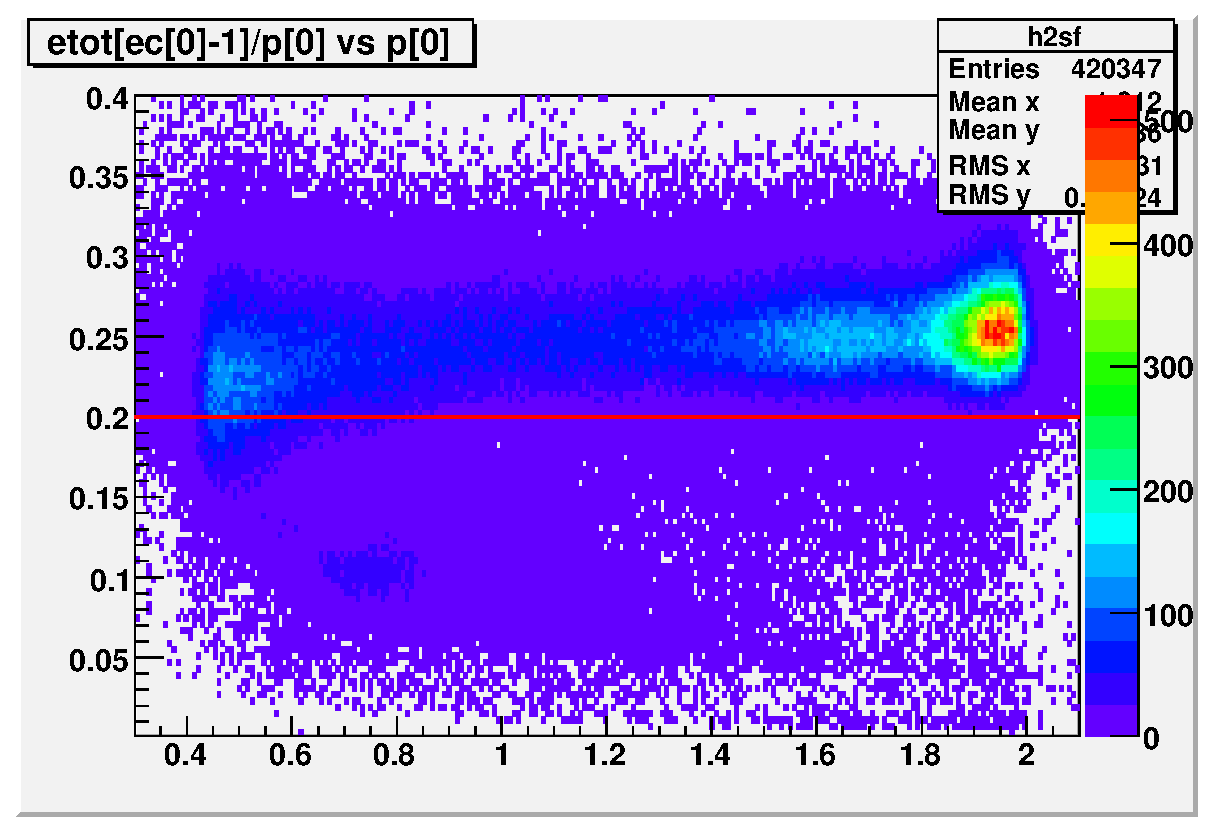
\includegraphics[width=1.0\textwidth]{figuresEG4/FigCuts/ecCuts_sfVp2D_Eb2allEv.eps}  %2.0 GeV data
\leavevmode 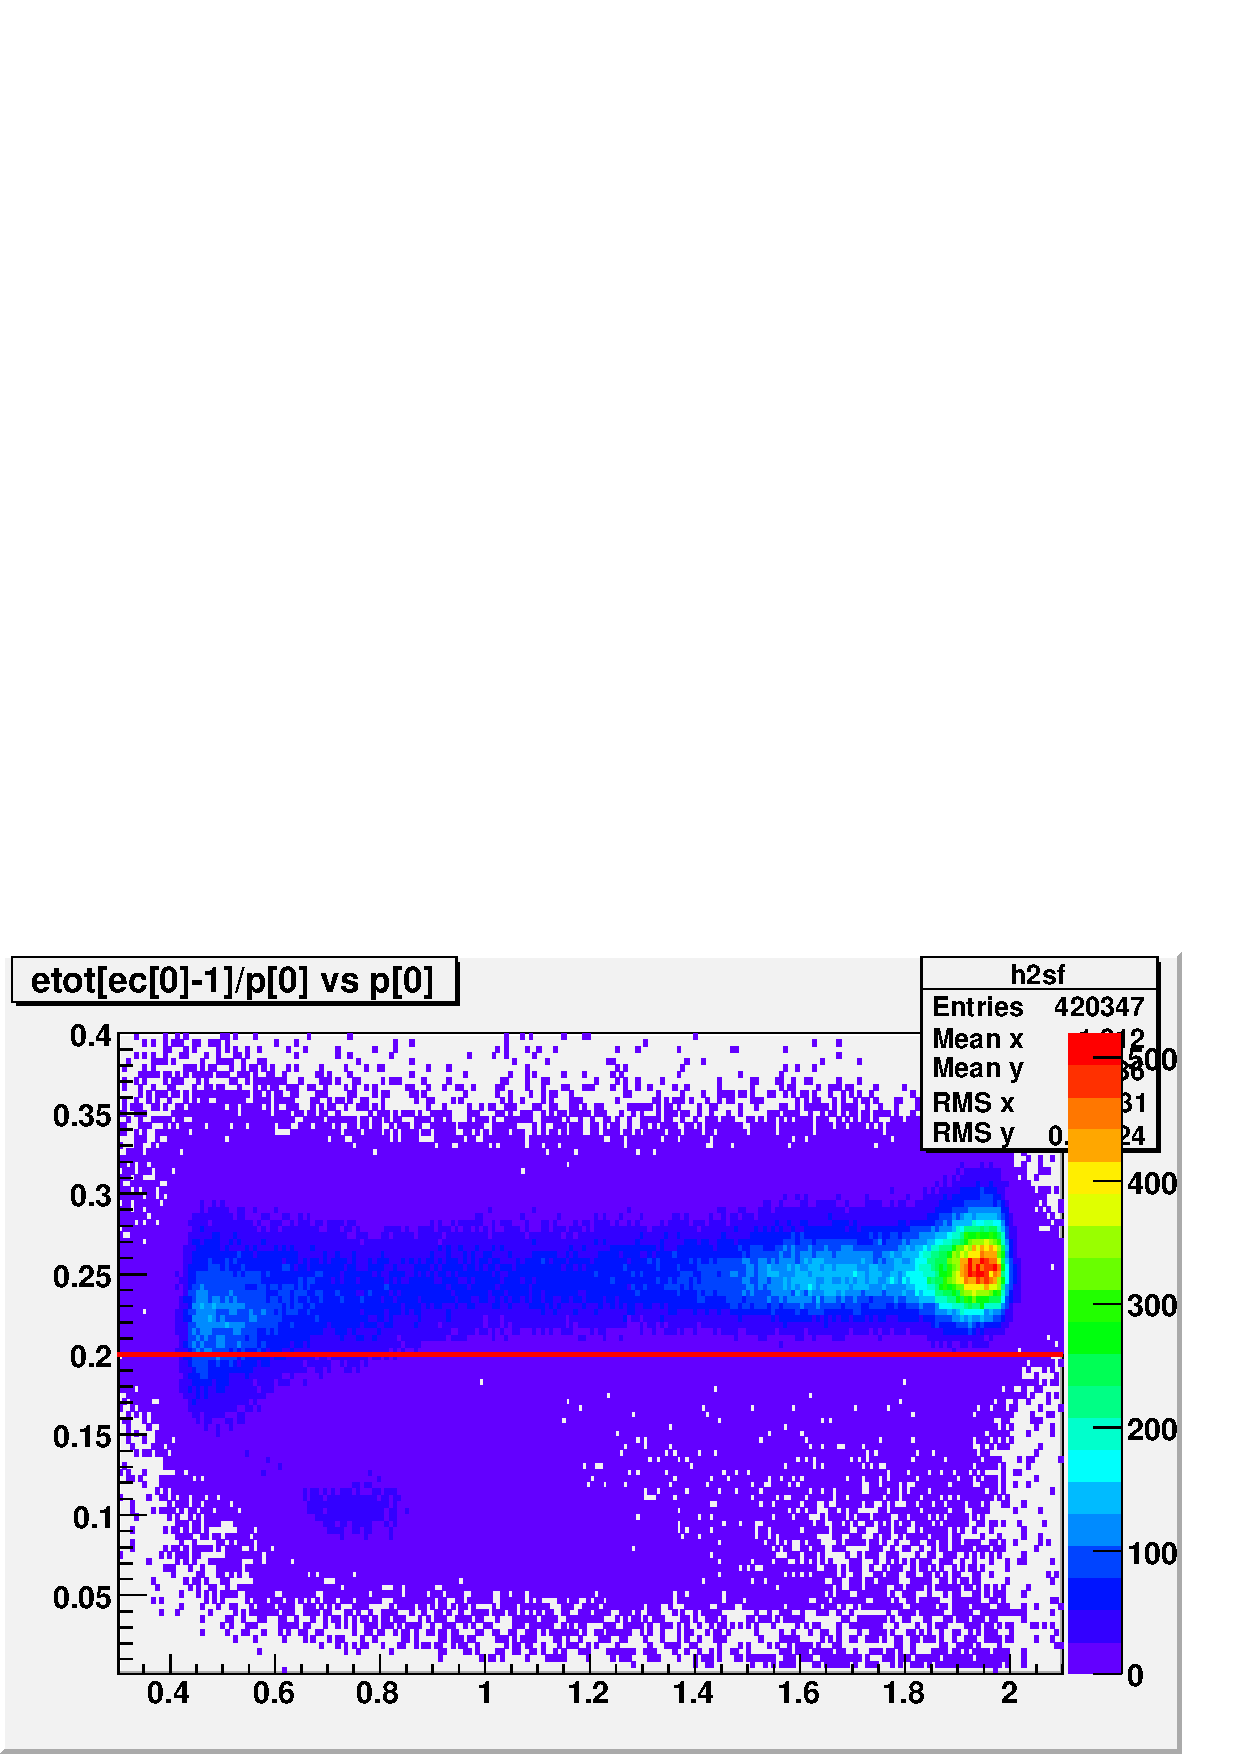
\includegraphics[width=0.8\textwidth]{figuresEG4/FigCuts/ecCuts_sfVp2D_Eb2allEv.png}  %2.0 GeV data
\caption[EC sampling fraction cut (2.0 GeV)]{An example of the cut on the EC sampling fraction (2.0 GeV data). The plots shows the distribution of the sampling fraction (in Y-axis) plotted against the particle momentum (in X-axis). The brighter stripe above about 0.2 in the energy fraction are due to the electrons whereas those below are the pions.
 %\textcolor{red}{SEK: Y-label (Sampling fraction); arrow/or texts indicating pions and electrons. This figure is not very clear - could you use logarithmic z scale? \\ GED: What are the exes? Units? What do we see here?}
}
\label{ecSf}
\end{figure}


%In case of EC in the CLAS, 
For the EC in CLAS, the electron sampling fraction ($etot/p$) is about 0.25 and pions give signals that are mostly below 0.2 (see Fig. \ref{ecSf} or others that follow). Therefore, a lower cut of $etot/p > 0.2$ is usually chosen to reject most of the pions without significantly losing good electrons. However, in %the case of 
our low beam energy experiment, %with its low beam energy, %being relatively smaller, 
few pions are produced and the electron peaks are cleaner in lower kinematic bins as can be seen in the low \qsqs bins of Fig. \ref{ecSfExp6}. Therefore, %in order to have fewer good electrons rejected, 
a \qsqs bin dependent cut of $etot/p > (\mu - 3\sigma)$ was chosen, where $\mu$ and $\sigma$ are the Gaussian fit parameters representing the mean and standard deviation of the distribution in the corresponding \qsqs bin. 
The choice of $3 \sigma$ was decided by looking at the sampling fraction distributions in each of the \qsqs bins and making sure that no pion signal was observed in any of the bins.


On simulated data also, a corresponding $3 \sigma$ cut was applied by first repeating the exact same procedure to get the corresponding values of $\mu$ and $\sigma$ from the simulated data. Using same-$\sigma$ cuts %(i.e. the same relative distance from the electron peaks) 
in corresponding \qsqs bins of both experimental and simulated data ensures that we had the same fraction of data in corresponding bins from both experimental and simulated sides. 



\begin{figure}[H]%[htp] %ht, htpb (p - float, b = bottom, h=? t = top)
\centering
%\leavevmode 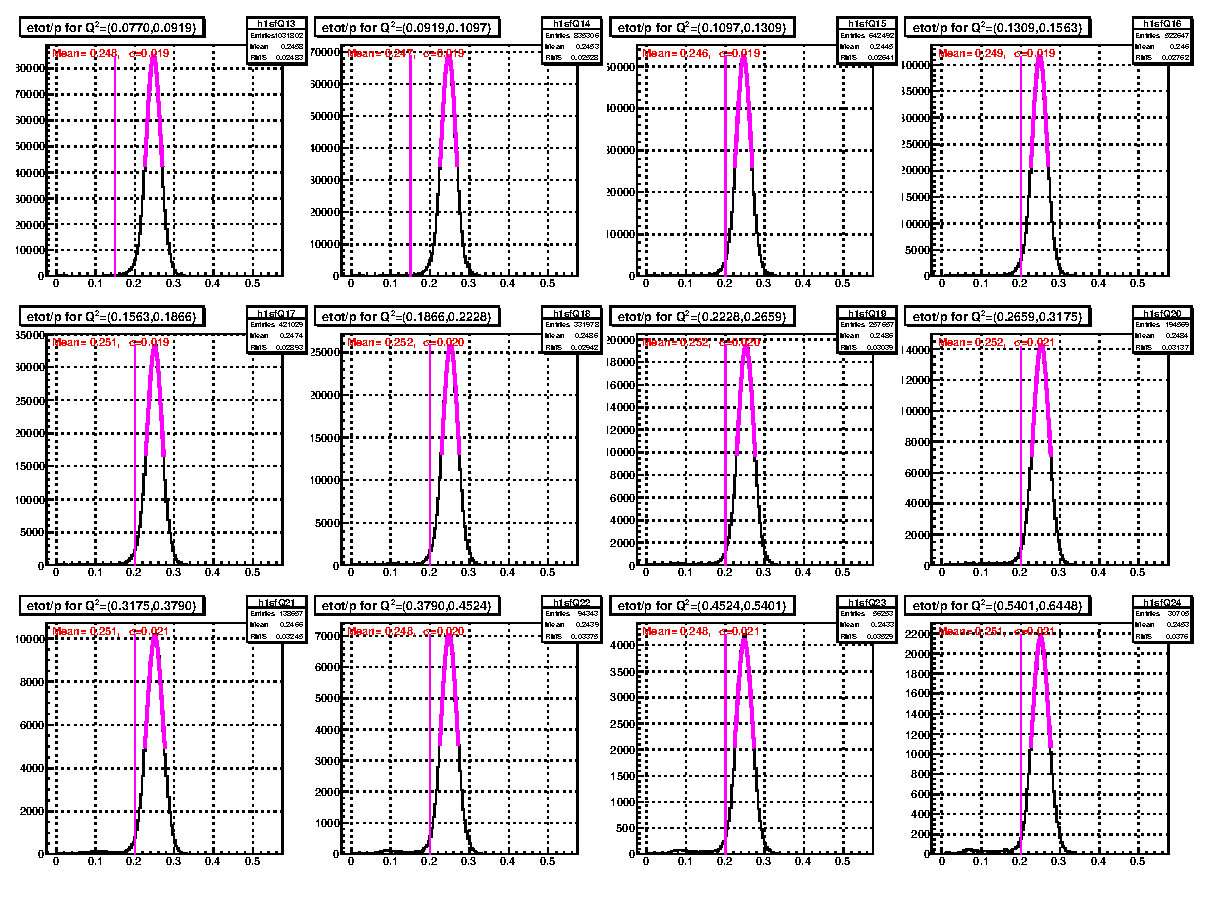
\includegraphics[width=1.0\textwidth]{chap4simul/FigCuts/ecCuts_sfOneD_Eb2_4Th.eps}  %0.6 is the fraction of the real image width????
%\leavevmode 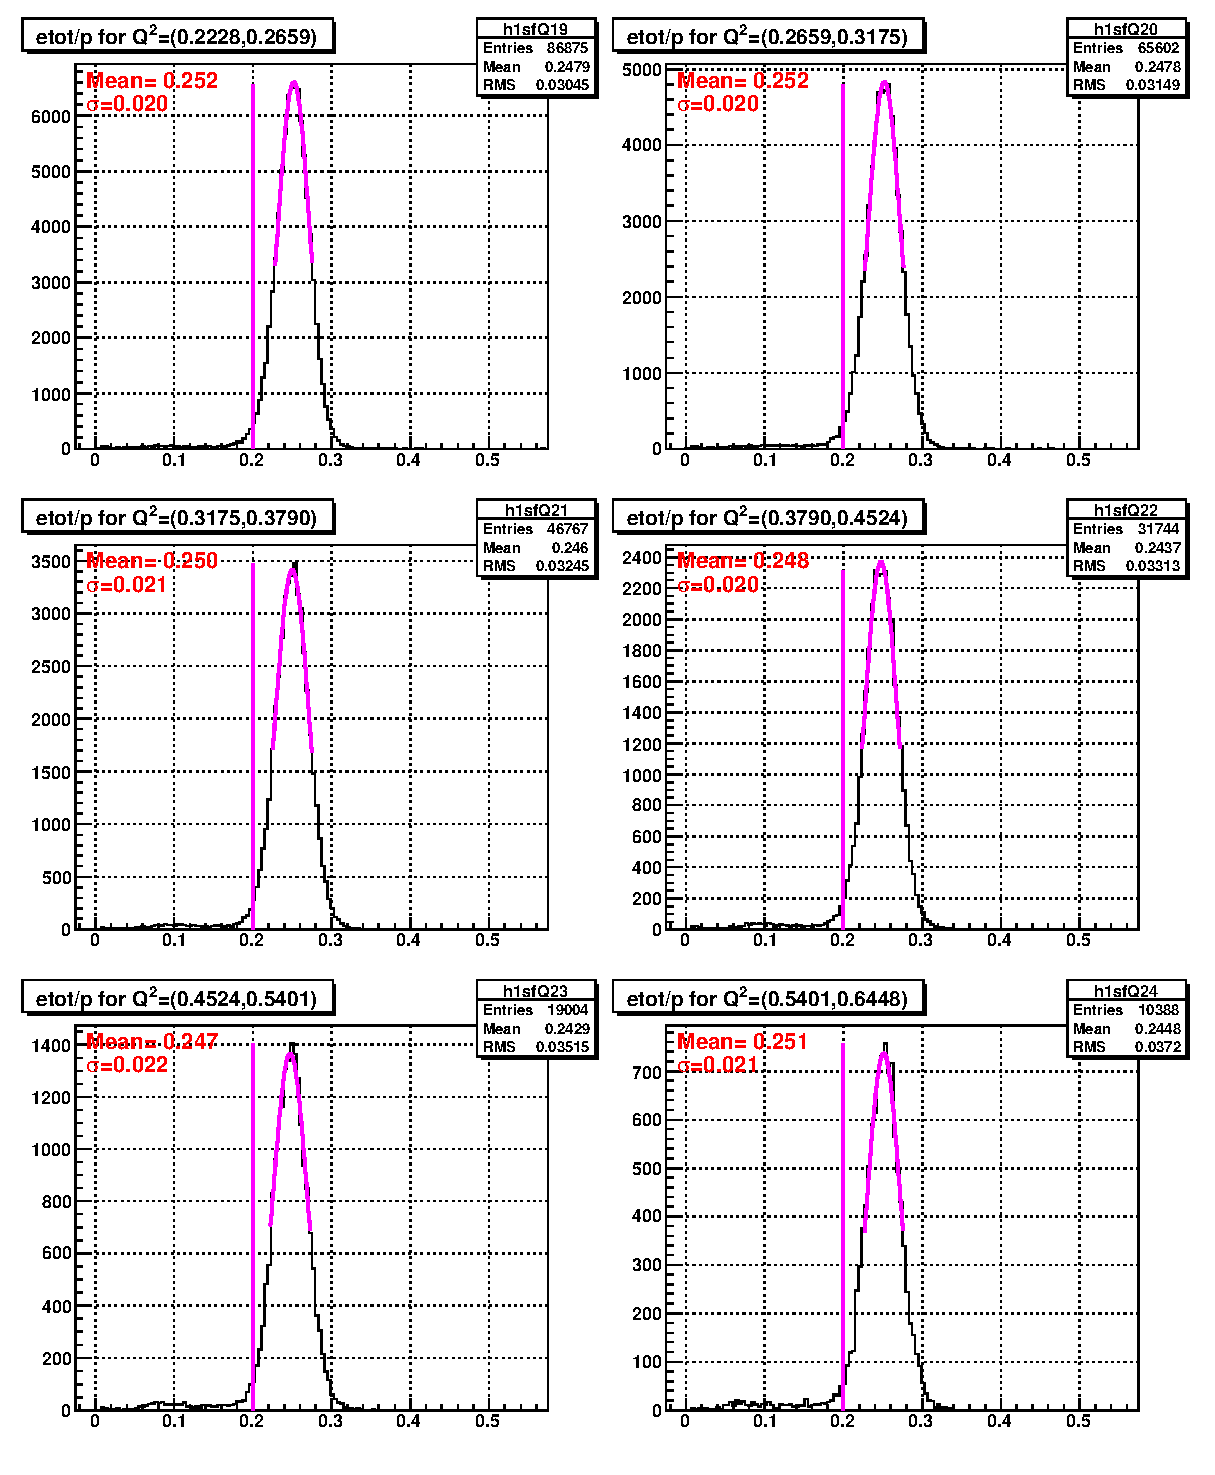
\includegraphics[width=1.0\textwidth]{chap4simul/FigCuts/ecCuts_sfOneD_Eb2_4ThN.eps}  %0.6 is the fraction of the real image width????
\leavevmode 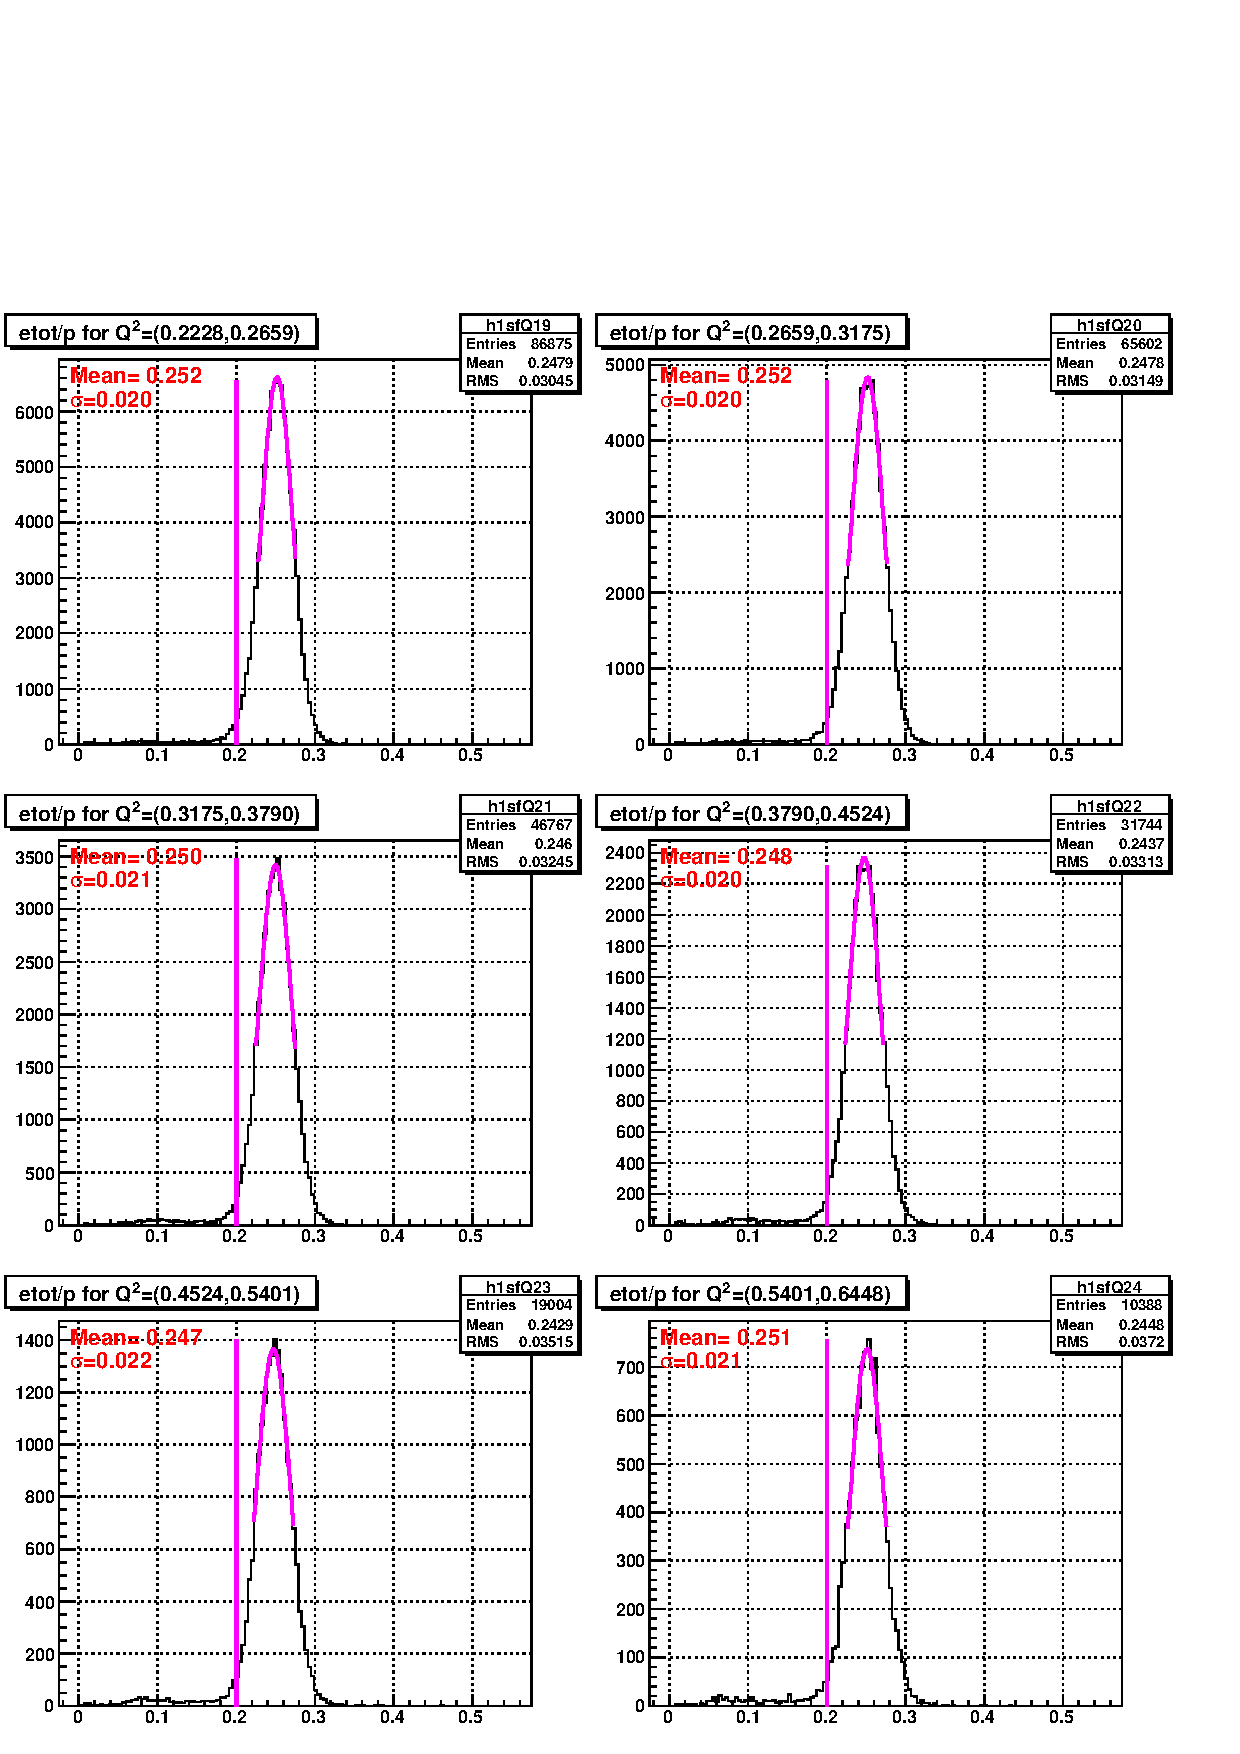
\includegraphics[width=1.0\textwidth]{figuresEG4/FigCuts/ecCuts_sfOneD_Eb2_4ThN.png}  %0.6 is the fraction of the real image width????
\caption[EC sampling fraction cut (Exp.)]{The \qsqs dependent cuts on the EC sampling fraction for 2.0 GeV experimental data. Events below the red lines are rejected.}
\label{ecSfExp6}
\end{figure}



\begin{figure}[H]%[htp] %ht, htpb (p - float, b = bottom, h=? t = top)
\centering
%\leavevmode 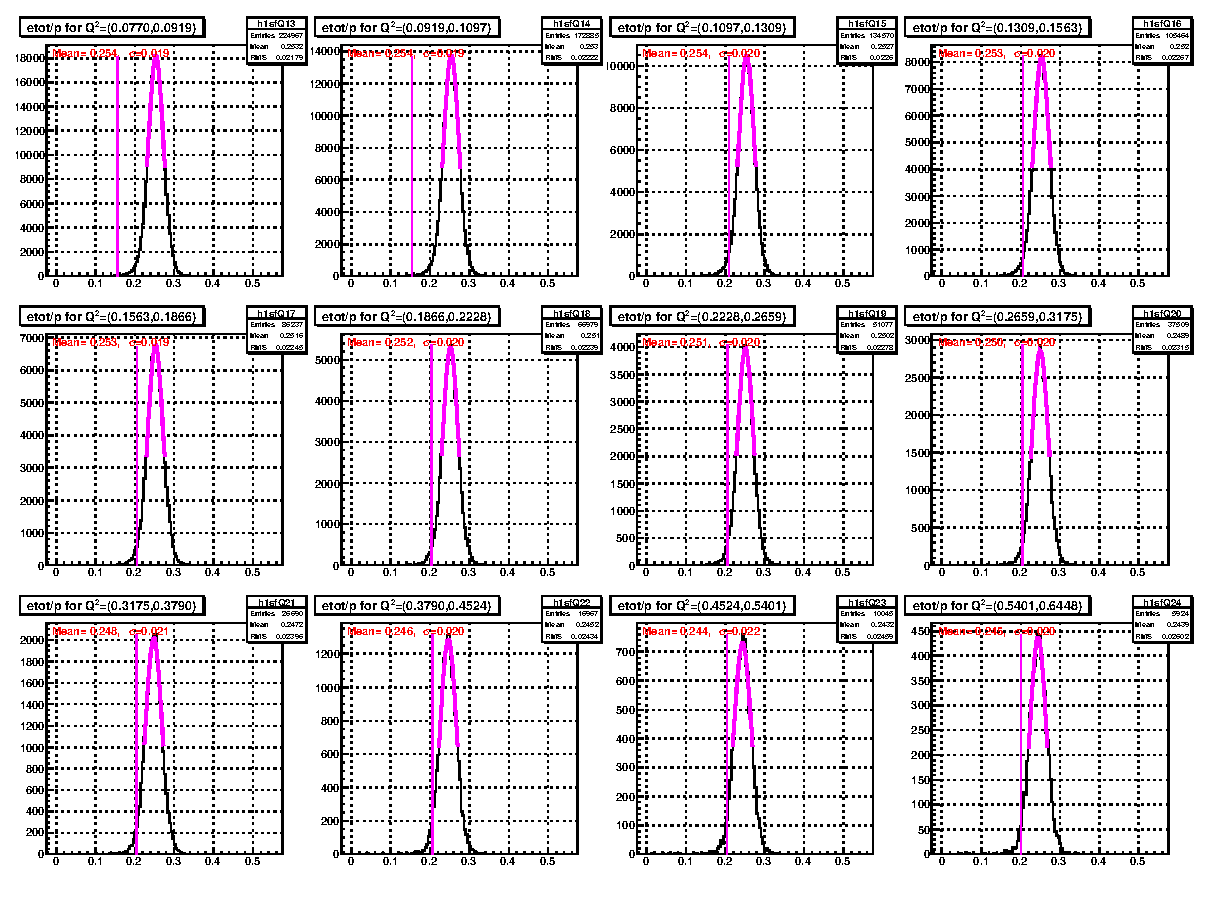
\includegraphics[width=1.0\textwidth]{chap4simul/FigCuts/ecCuts_sfOneD_Eb2_4Thsim.eps}  %0.6 is the fraction of the real image width????
%\leavevmode 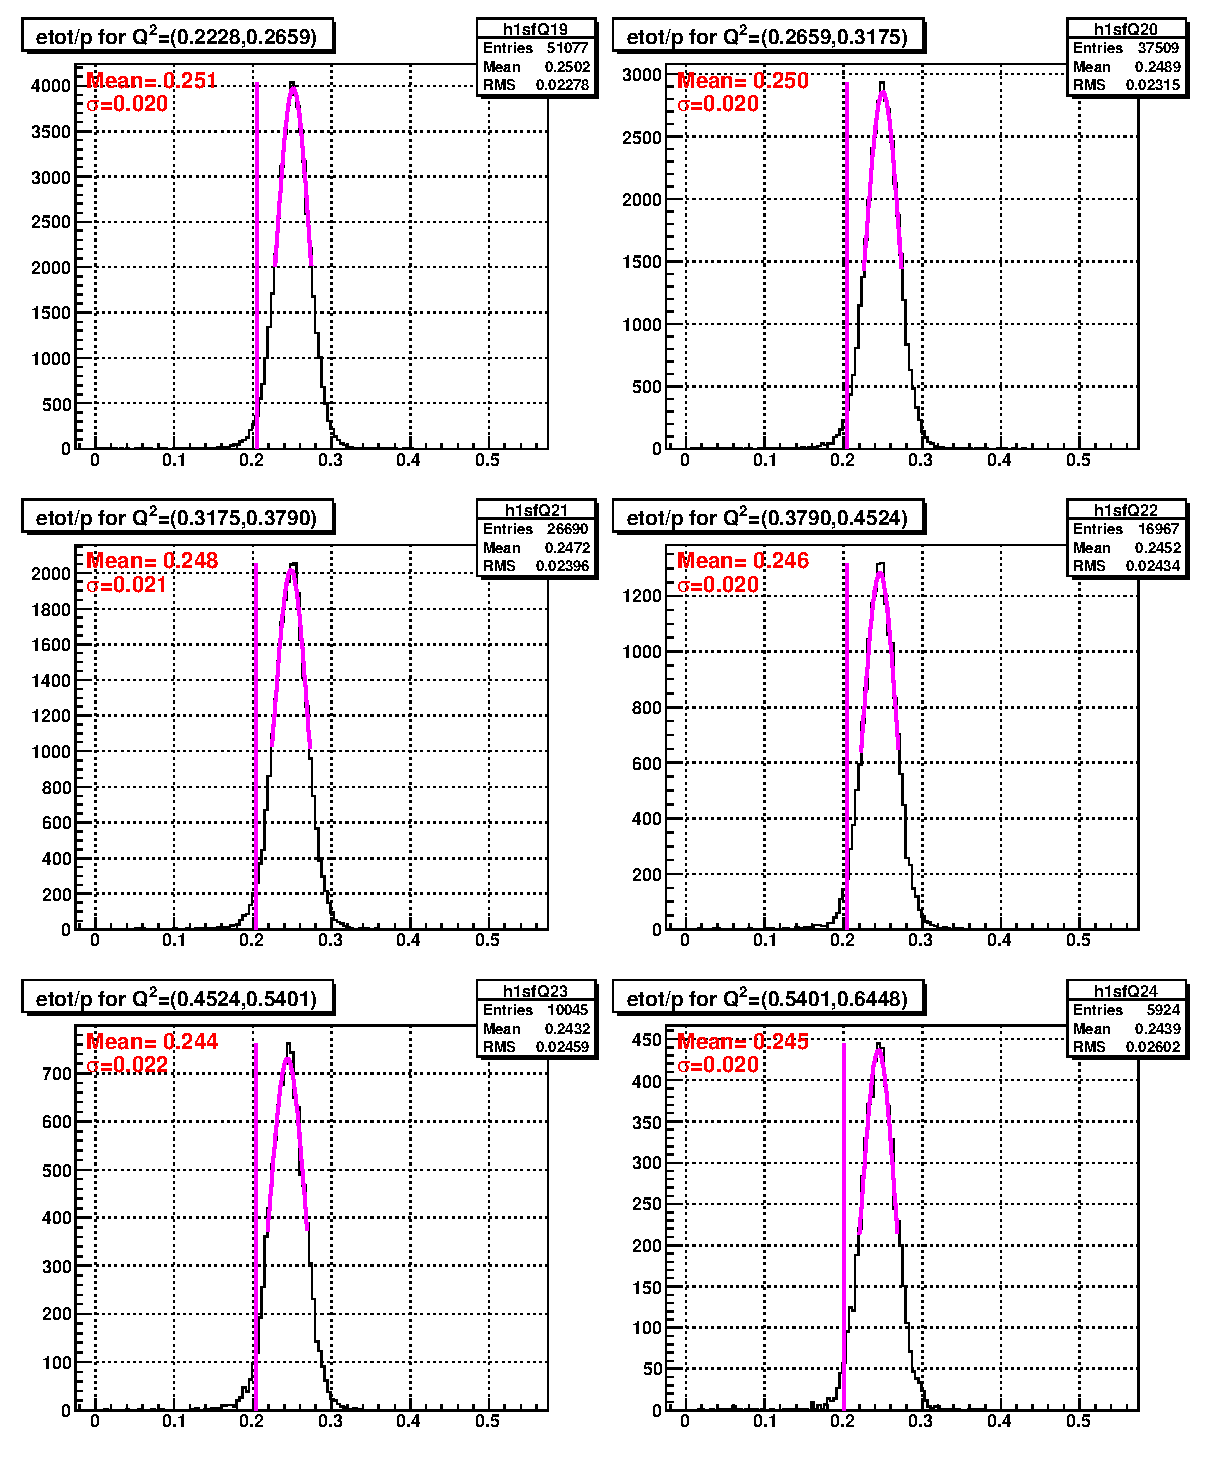
\includegraphics[width=1.0\textwidth]{chap4simul/FigCuts/ecCuts_sfOneD_Eb2_4ThsimN.eps}  %0.6 is the fraction of the real image width????
\leavevmode 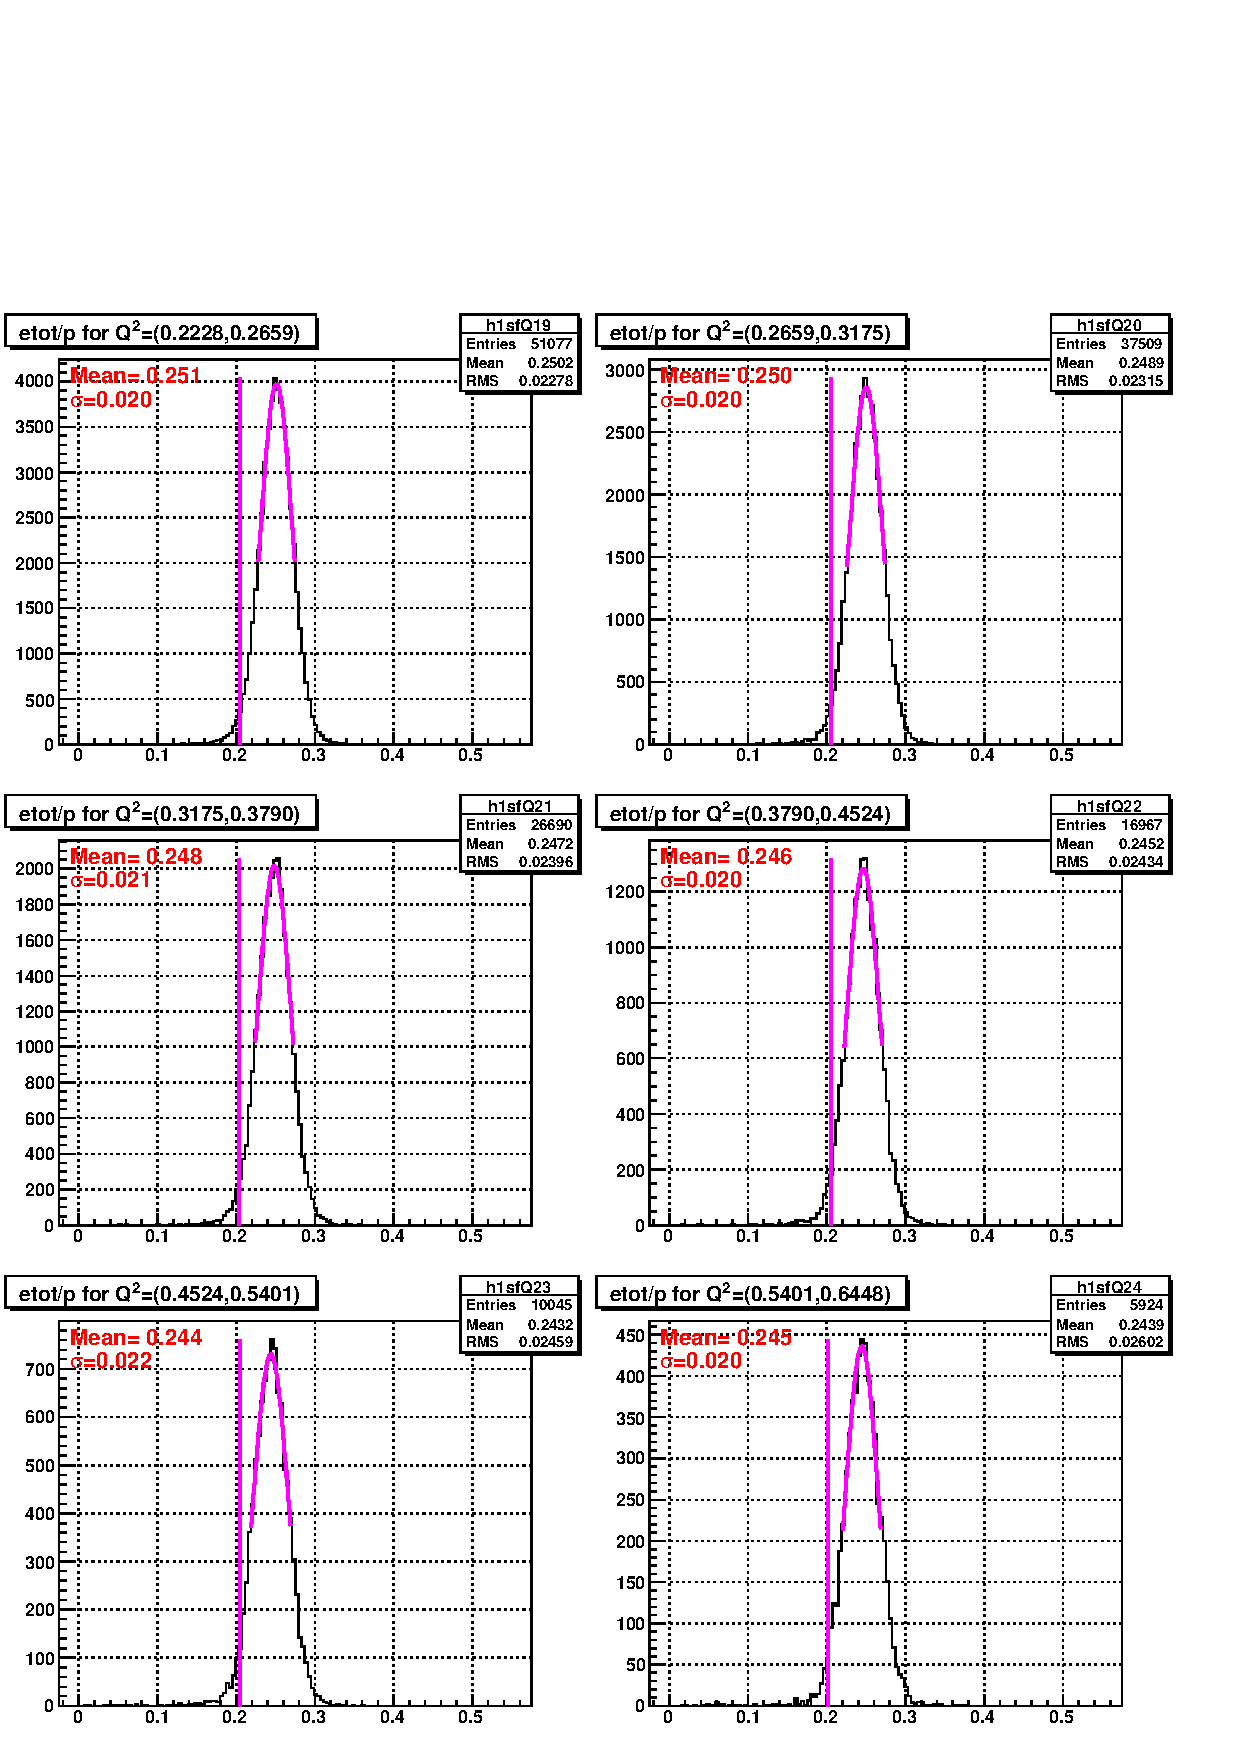
\includegraphics[width=1.0\textwidth]{figuresEG4/FigCuts/ecCuts_sfOneD_Eb2_4ThsimN.png}  %0.6 is the fraction of the real image width????
\caption[EC sampling fraction cut (Sim.)]{The \qsqs dependent cuts on the EC sampling fraction for 2.0 GeV simulation data. Events below the red lines are rejected.}
\label{ecSfSim6}
\end{figure}


%In short, only two numbers 0.15 and 0.2 define the cuts on the experimental data, but the cuts for simulation data are all different, yet they are at the same relative distance from the electron peaks as in the experimental data and, therefore, include about the same fraction of good electrons. 

%\textbf{\textcolor{red}{This section may have been too verbose and complex to understand.}}
% http://en.wikipedia.org/wiki/Particle_shower:   An ``electromagnetic shower'' begins when a high-energy electron, positron or photon enters a material. At high energies (above a few MeV, below which photoelectric effect and Compton scattering are dominant), photons interact with matter primarily via pair production  that is, they convert into an electron-positron pair, interacting with an atomic nucleus or electron in order to conserve momentum. High-energy electrons and positrons primarily emit photons, a process called bremsstrahlung. These two processes (pair production and bremsstrahlung) continues until photons fall below the pair production threshold, and energy losses of electrons other than bremsstrahlung start to dominate. 
%In the case of experimental data, the sampling fraction is cut at 0.2 in the first fourteen \qsqs bins and at 0.15 in the others. But, in the case of simulated data, the cuts are variable, but still are correlated with the cuts on the real data. To ensure the proportional/same fraction of events from both real and simulated data in a given \qsqs bin, the electron peaks on those data are first fitted to Gaussian distributions to find the peak position and width (represented by $\sigma$ i.e. the standard deviation), and then cut position on simulated data is determined by the value which is at the same distance from  the average in terms of $\sigma_{sim}$ as the cut on real data is from its own mean in terms of $\sigma_{exp}$.






\subsubsection{Cuts on $E_{in}$}
\begin{figure}[h] %ht, htpb (p - float, b = bottom, h=? t = top)
\centering
%\leavevmode 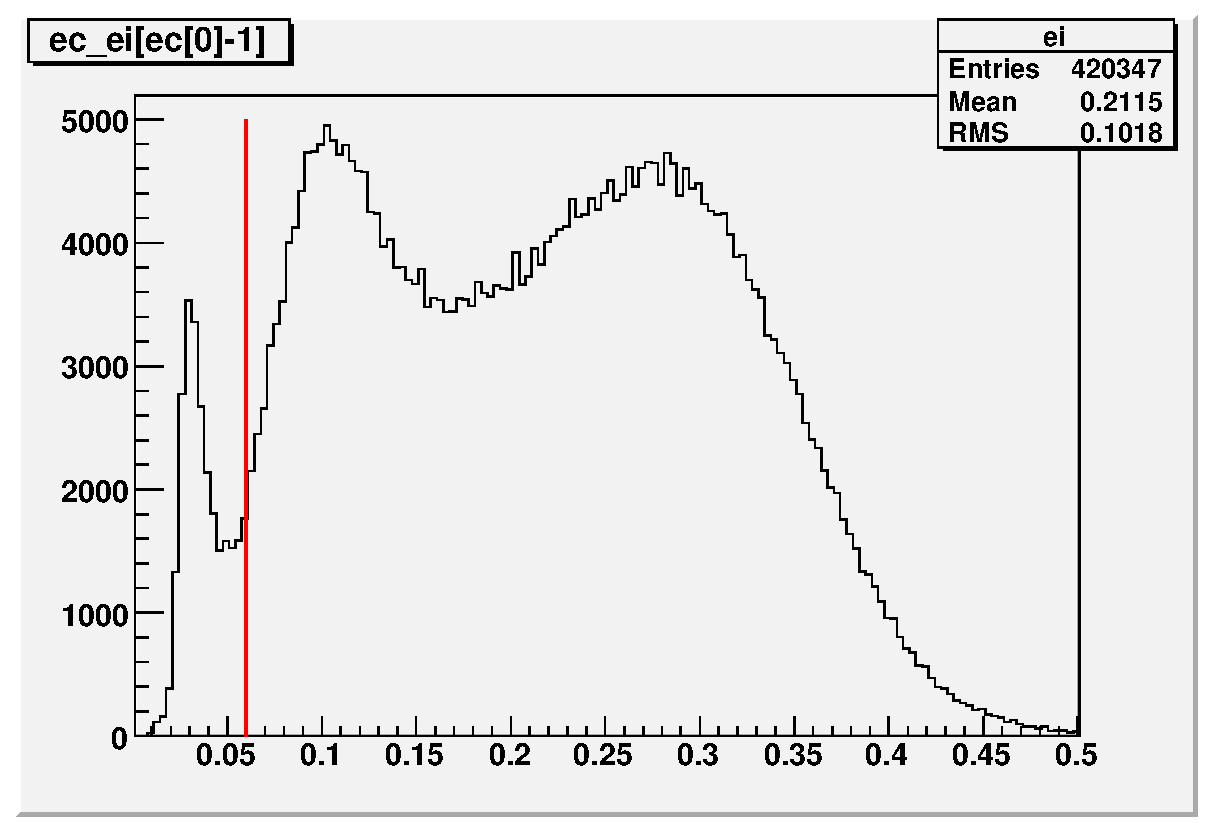
\includegraphics[width=0.8\textwidth]{chap4simul/FigCuts/ec_eiCutFrmRtPrmtClasEb2.eps}  %0.6 is the fraction of the real image width????
\leavevmode 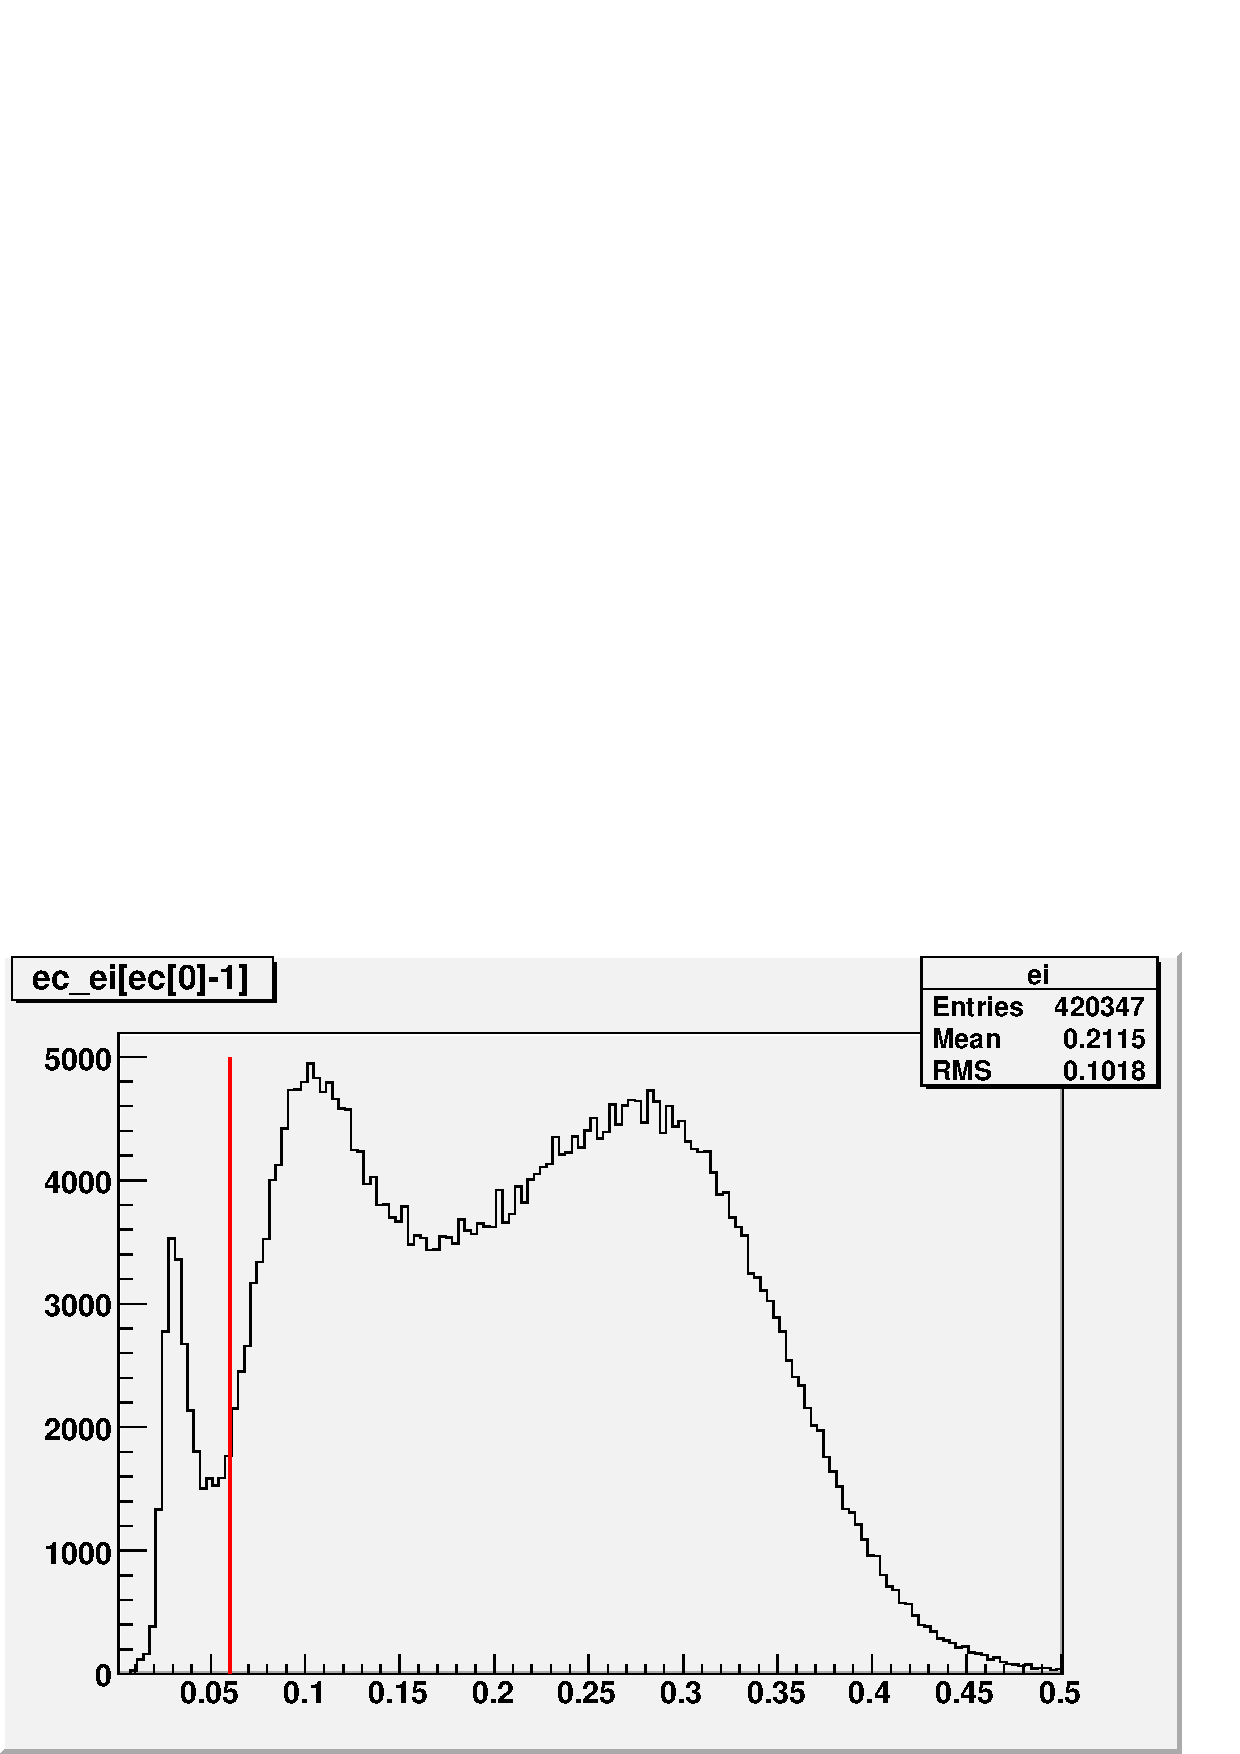
\includegraphics[width=0.8\textwidth]{figuresEG4/FigCuts/ec_eiCutFrmRtPrmtClasEb2.png}  %0.6 is the fraction of the real image width????
\caption[EC inner energy cut (2.0 GeV)]{Energy deposited (GeV) in the inner EC and the cut (red line) used to reject pions (seen as a peak at about 0.03 GeV) from a sample of electron candidates of 2.0 GeV data.}
\label{ecInExp1}
\end{figure}

Pions, which do not shower and are minimum ionizing particles in the momentum range detected in CLAS, deposit only a small amount of energy in the inner part of the EC, %in the ratio of about 5:3, independent on their momentum. %https://userweb.jlab.org/~ungaro/maureepage/proj/pi0/e_pid/note/electron_pid.html#x1-100001.7
independent of their momentum. When $E_{in}$ is histogrammed, the small pion signal peak at about 0.03 clearly stands out from the large electron sample, with little overlap in between. So, a universal cut of $E_{in}$=0.05 on both data and simulation (as shown in Figs. \ref{ecInExp1}, \ref{ecInExp6} and \ref{ecInSim6}) safely rejects most of the pions from the electron candidate sample. 


\begin{figure}[H]%[hp] %ht, htpb (p - float, b = bottom, h=? t = top)
\centering
%\leavevmode 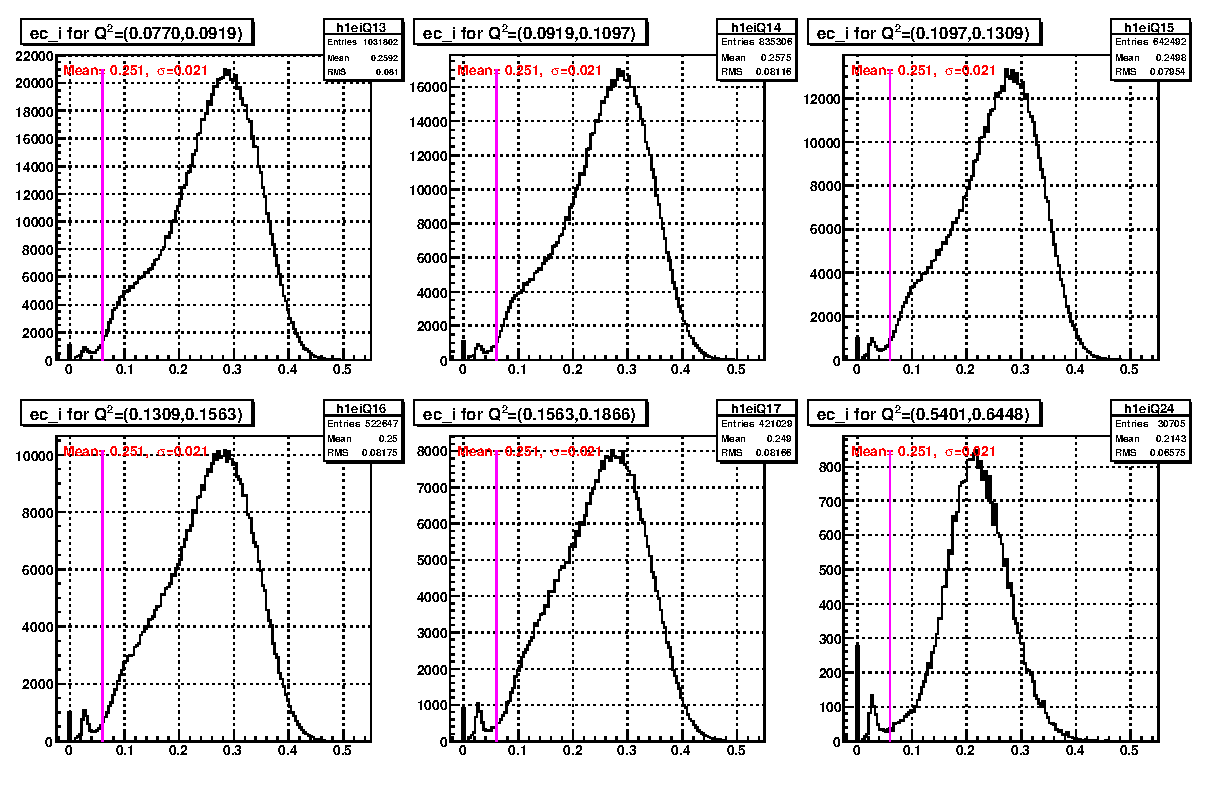
\includegraphics[width=1.0\textwidth]{chap4simul/FigCuts/ecCuts_eiOneD_Eb2_4Th.eps}  %0.6 is the fraction of the real image width????
\leavevmode 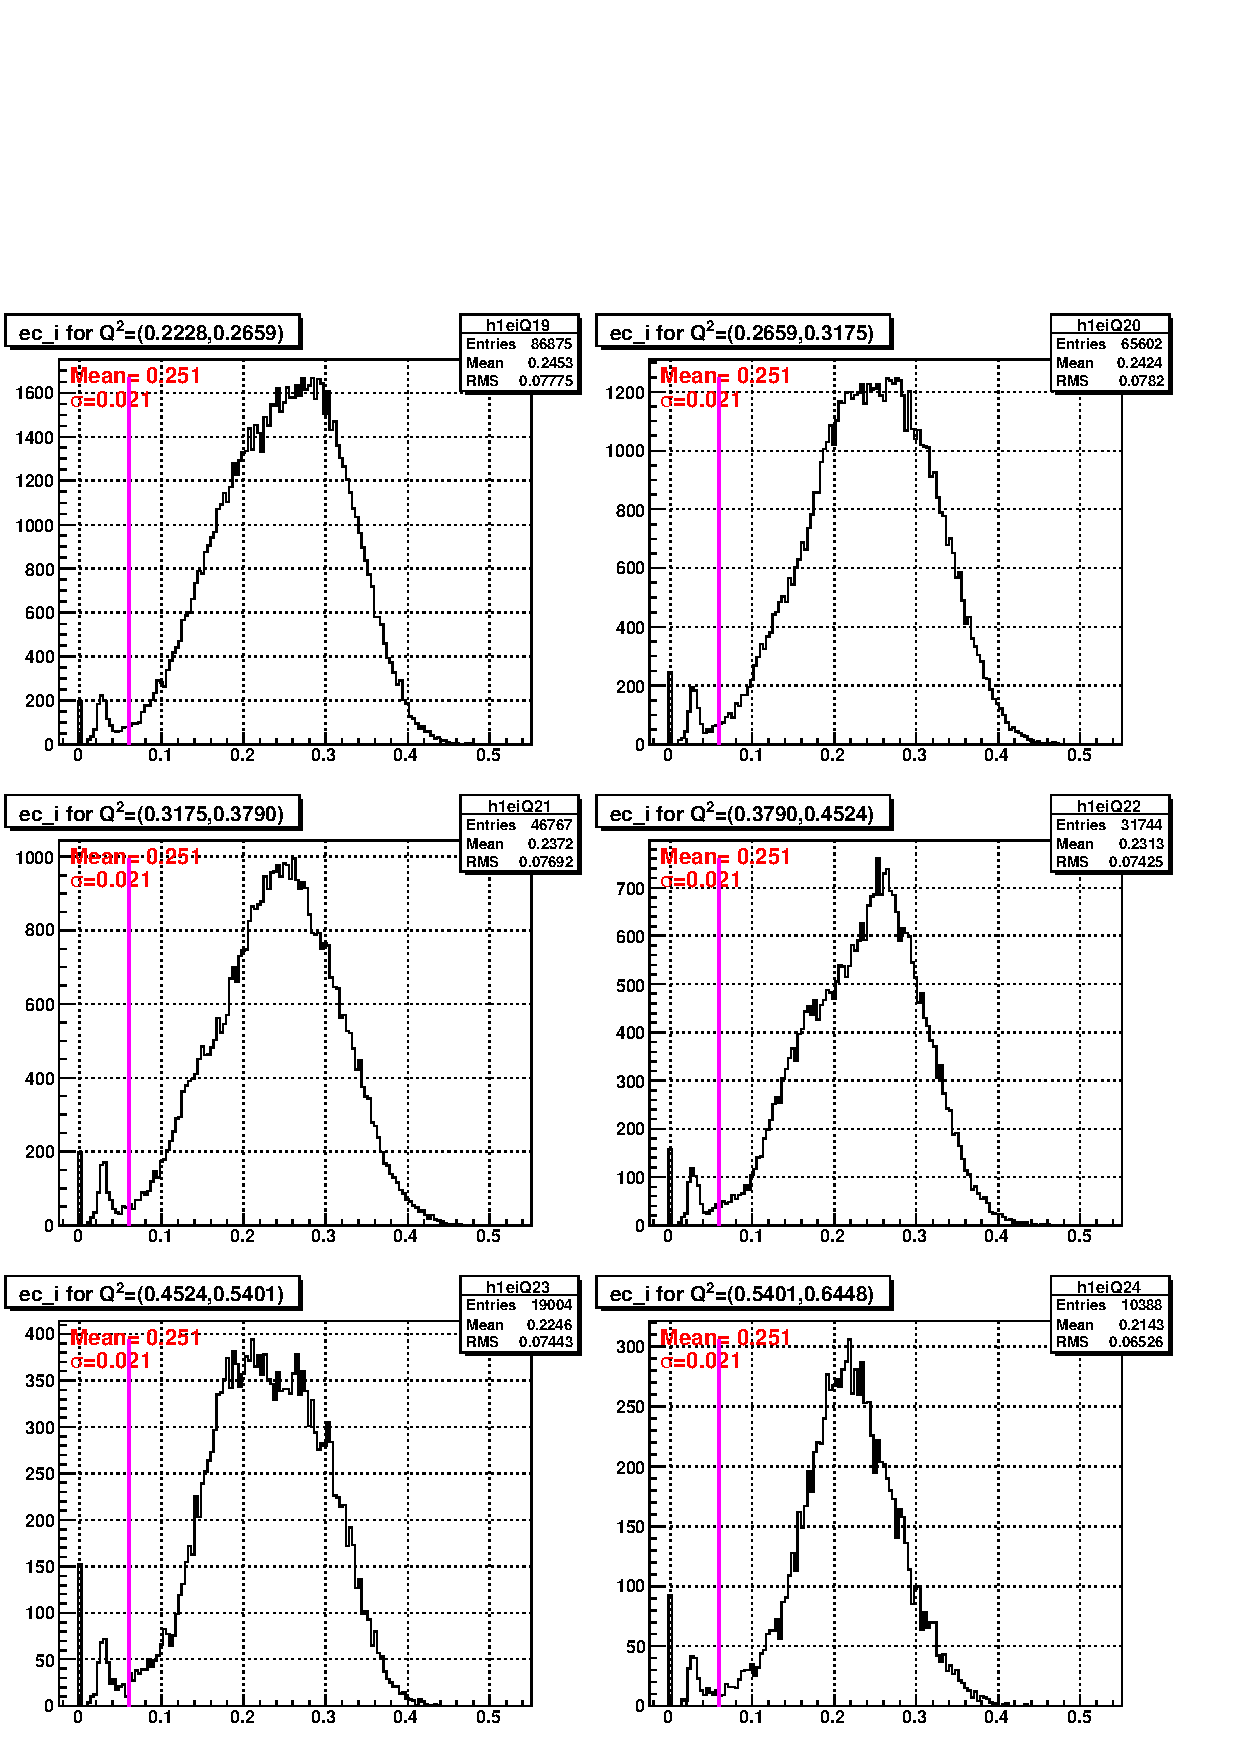
\includegraphics[width=1.0\textwidth]{figuresEG4/FigCuts/ecCuts_eiOneD_Eb2_4ThN.png}  %0.6 is the fraction of the real image width????
\caption[EC inner energy cut (Exp.)]{The EC-inner cut on a sample of 2.0 GeV experimental data in various \qsqs bins.}
\label{ecInExp6}
\end{figure}



\begin{figure}[H]%[hp] %ht, htpb (p - float, b = bottom, h=? t = top)
\centering
\leavevmode 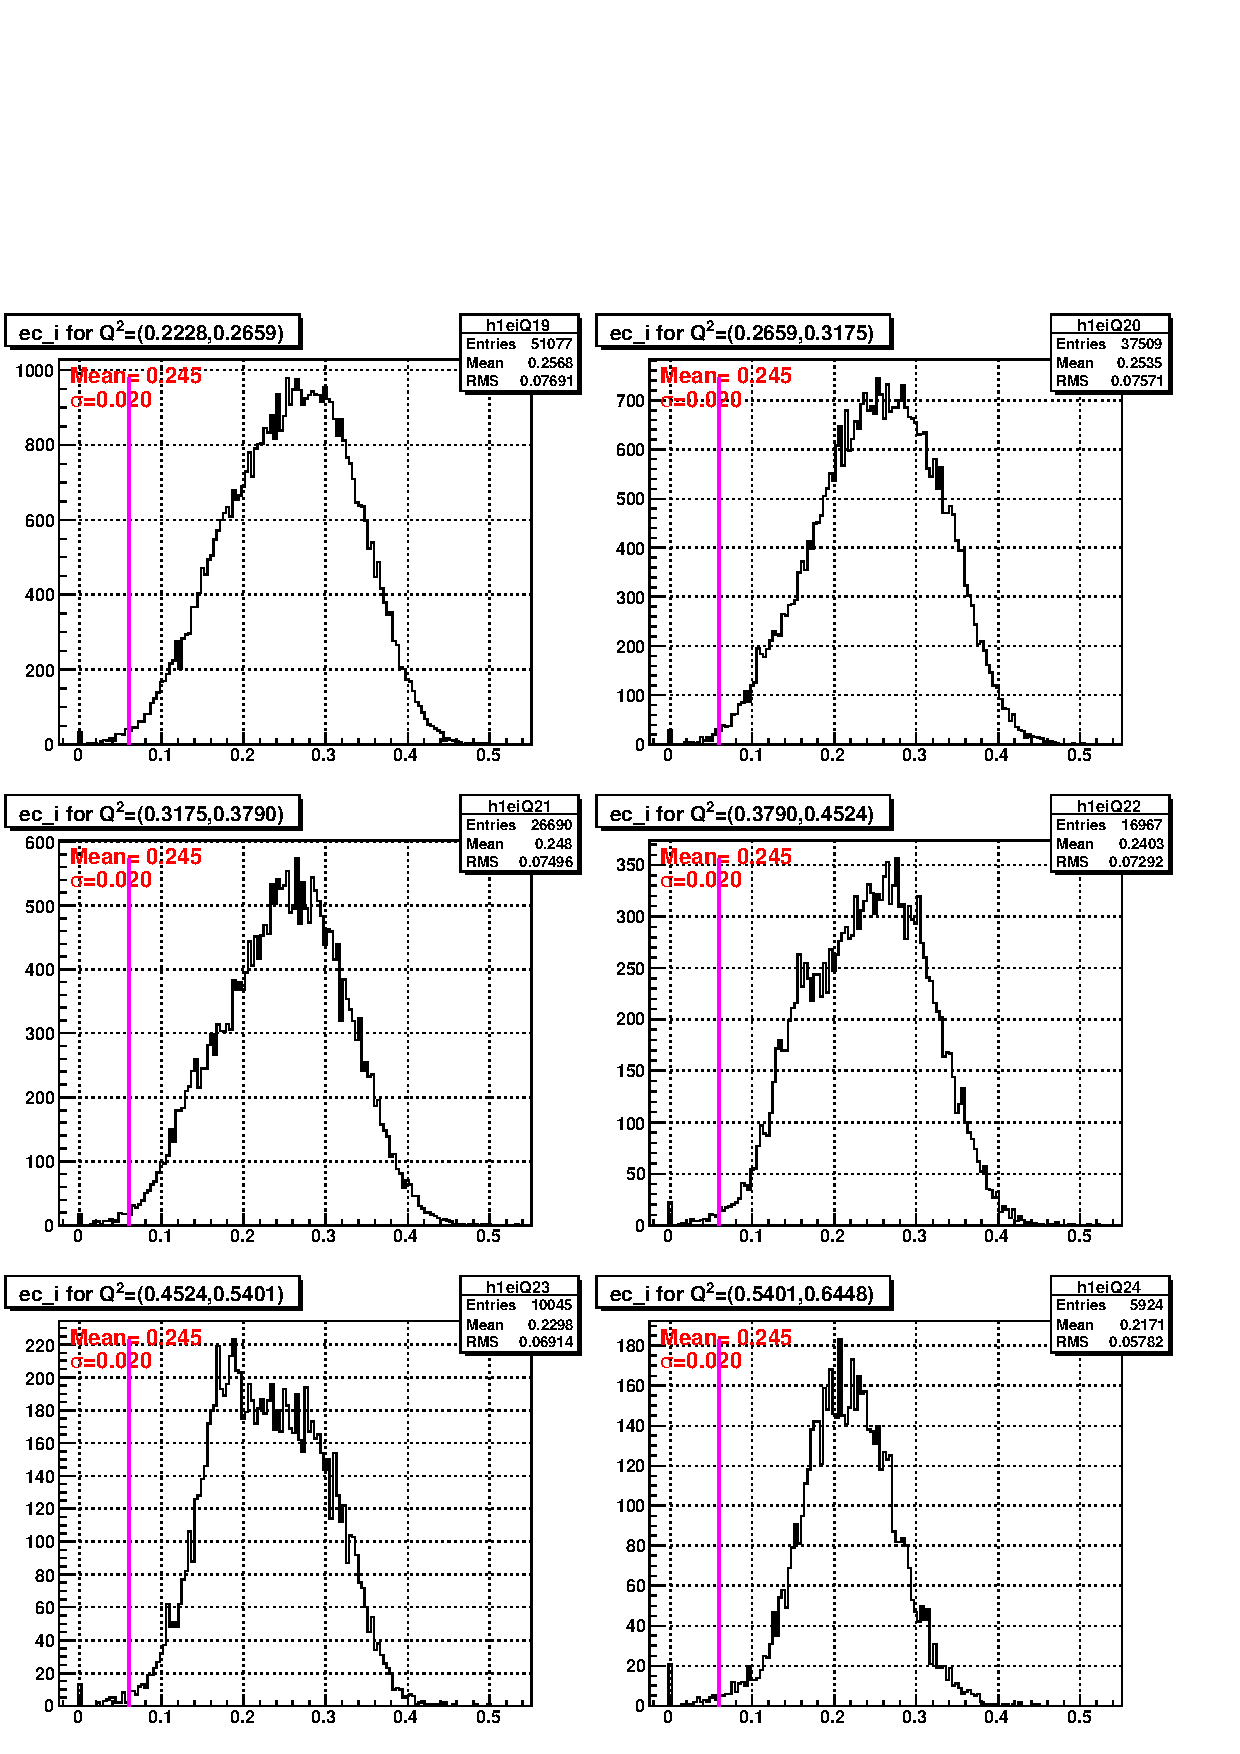
\includegraphics[width=1.0\textwidth]{figuresEG4/FigCuts/ecCuts_eiOneD_Eb2_4ThsimN.png}  %0.6 is the fraction of the real image width????
\caption[EC inner energy cut (Sim.)]{The EC-inner cut on a sample of 2.0 GeV simulation data in various \qsqs bins.}
\label{ecInSim6}
\end{figure}




\begin{comment} %Part copied from my thesis (just to remind myself what I had done)

\subsubsection{Cuts on $E_{out}$}
In addition to the two EC-cuts above, one more cut based on the correlation between EC-outer and EC-inner %ec\_o/p and ec\_i/p 
(as shown in Fig. \ref{ecOvI}) was used which helps further to clean up the electron sample. %pion contamination. %%%SEK cor.

\begin{figure}[H]%[h] %ht, htpb (p - float, b = bottom, h=? t = top)
\centering
\leavevmode 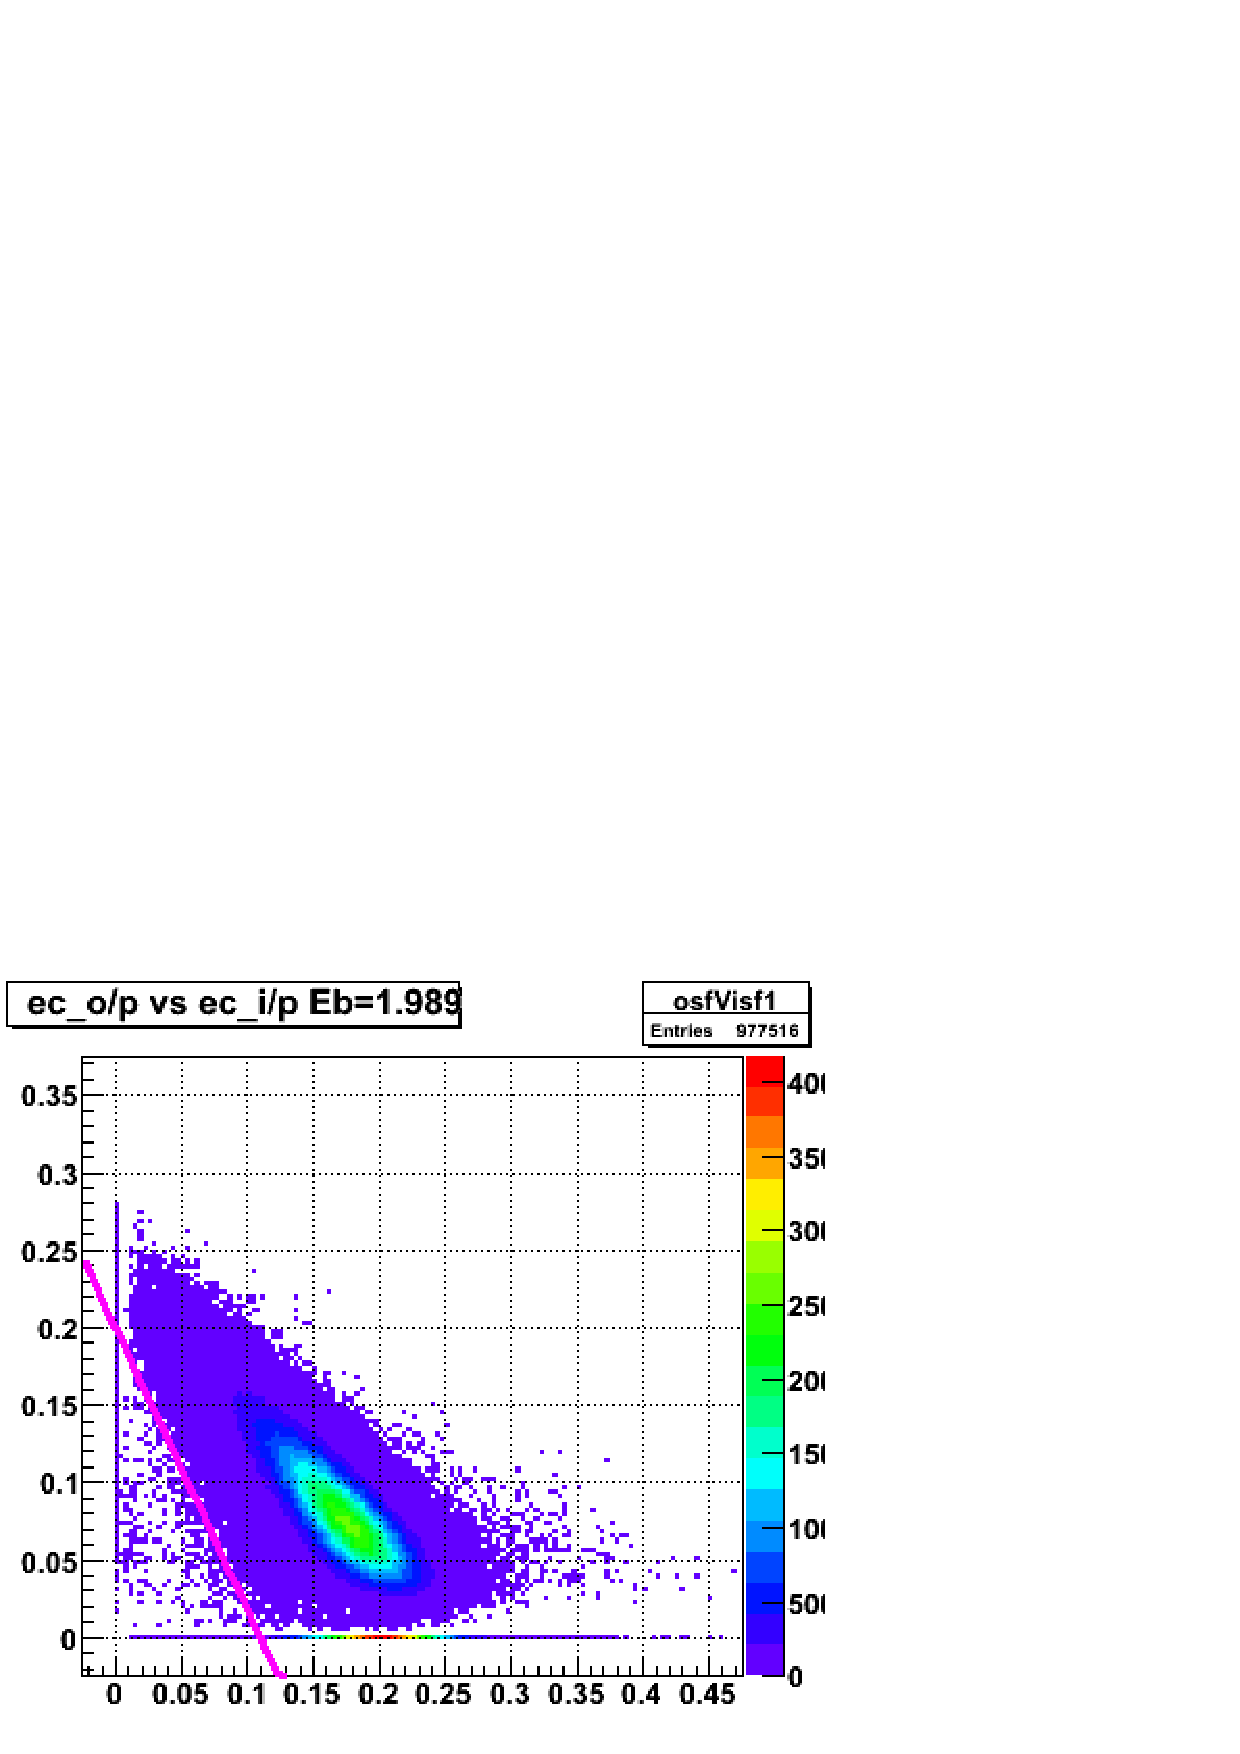
\includegraphics[width=0.8\textwidth]{figuresEG4/FigConv/stdECcutsSfovSfi_Eb2sim.png}  %0.6 is the fraction of the real image width????
\caption[EC inner and outer energy cut (Exp.)]{Energy detected in EC outer as a function of EC inner, both normalized with the particle momentum, for the 2 GeV data. The brown line shows the EC cut to reject pions (which fall below that line).}
\label{ecOvI}
\end{figure}

\end{comment}

\subsection{Cerenkov Counter Cuts}
\subsubsection{ Osipenko (CC Geometry and Time Matching) Cuts}
\label{osiCuts}
As discussed in Sec. \ref{cha:EG4} %{expSetUp} %Or refer directly to the CC section (by its own label, to be added)  (There were 18 modules in the old CC of of each CLAS sector)
the new EG4-dedicated CC consists of 11 modules %/segments 
each consisting of a pair %each 
of mirrors and PMTs. The segments are placed along the CLAS polar angle covering 15 to 45 degrees, i.e., the segments are at different polar angular positions. % See presentation cerenkov_son_july2003 (in the UbuntuOne/EG4nMore1/Jlab/Detector/CLASdetector/CC (also have a look at other presentations as well as E. Golovach's work on the Cerenkov (linked from EG4 wiki main page - http://www.ge.infn.it/~golovach/cerenkov/ (I can/may find a lot of plots and design diagrams))
During normal operation, the PMTs of these segments may produce %a certain amount of noise signal 
thermal noise that is equivalent to that produced by one photo-electron passing through it. As a result, when a noise pulse in the CC and a pion track measured by DC coincides within the trigger window of the CLAS detector, %Nevzat writes the window is 150 ns; thesis pg 145
the track gets registered as an electron candidate by the event reconstruction program, thus contributing to the contamination of electron candidates % samples 
with the misidentified pion tracks. In fact, this turns out to be the biggest source of pion contamination. In order to minimize such contamination and help better identify electrons from pions, %the 
CC geometric and time-matching cuts are applied.

%https://userweb.jlab.org/~ungaro/maureepage/proj/pi0/e_pid/note/electron_pid.html#x1-120001.9
%The cuts in this category
This category of cuts for this experiment is %by X. Zheng \cite{eg4wiki} - one of the collaborators of the experiment. Her work, in turn, was 
mostly based on a similar analysis done for another CLAS experiment by M. Osipenko \cite{cnOsipenko, anaNoteXZheng}.% in order to study the CC response and thereby develop a method to better discriminate electrons from pions. 


The first requirement in the CC-matching is for the electron candidate track (as reconstructed by DC) to have a corresponding signal in CC. In addition, the track needs to meet several %the following %GED
matching conditions to be acceptable as described in the next sections.


%\subsubsubsection{CC \th Matching} %http://tex.stackexchange.com/questions/186981/is-there-a-subsubsubsection-command
\paragraph{CC \th Matching}
As said above, the CC segments are at different average polar angle positions (between 15 and 45 degrees), so in principle, one can expect a one-to-one correspondence between the polar angle of the track (as measured at the vertex) and the CC-segment. However, the torus magnetic field bends the particles towards or away from the beamline, so it's more convenient to use the CC projected polar angle \thp  rather than the vertex angle $\theta$, where \thp is defined as the polar angle of the position vector defined by the point of intersection of the track with %the CC plane
the plane at which the CC PMTs reside as reflected by the CC mirrors %xz: I think instead of "the CC plane" you should say "the plane at which the CC PMTs reside as reflected by the CC mirrors."
(another projected angle \php is the azimuthal angle of the same vector). These projected angles can be uniquely calculated for each track based on the DC %and CC 
signals of the track as well as the CC geometry information. To simplify the later analysis process, these projected angles for each track were calcuated during the final %/pass1 version  of the
 data reconstruction process and then saved in the output files %(in ntuple-10 format)
  just like all the other %usual 
 information for the events and particles. 
Finally, for the actual electrons a one-to-one correspondence between \thp and the segment number can be established, 
which discriminates against %while the same cannot be done for the 
background noise and the accidental pions (or any other negative charge candidates). For each segment, the \thp distribution (see Fig. \ref{ccThProjDist}) is fitted with a gaussian %+ second order polynomial distribution
to determine its mean ($\mu$) and width ($\sigma$) and then saved for future use in cuts. These fit parameters are then used during the data analysis to define these CC-\th-matching cuts. The events that have $\mu-3\sigma<\theta_{proj}<\mu+3\sigma$ pass this cut, and the others are rejected as not genuinely being electrons. %\textbf{\textcolor{red}{Plots later ..}}
% http://wwwold.jlab.org/Hall-B//secure/eg4/adhikari/Analysis/SimStuffs/CutsPlots/eg4CutsNCorrections.html#osiCuts
%      if(fabs(theta-th_offset[isec-1][iseg-1]) < (3.0*th_wid[isec-1][iseg-1]))        	theta_p_cut= true;
%      else                                                                             theta_p_cut= false;
\begin{figure}[H] %[hp] %ht, htpb (p - float, b = bottom, h=? t = top)
\centering
%\leavevmode \includegraphics[width=0.8\textwidth]{TexmakerMyFinTh/chap4simul/FigCuts/npheCutFrmRtPrmtClasEb2.eps}  %0.6 is the fraction of the real image width????
\leavevmode \includegraphics[width=1.0\textwidth]{TexmakerMyFinTh/chap4simul/FigCuts/ccOsipenkoXZhengNotePDFexportThProj}  %0.6 is the fraction of the real image width????
\caption[CC-projected \th distributions]{The \thp distributions %(from a carbon target run 50808) 
in two (9$^{th}$ and 10$^{th}$) of the CC-segments (figures used from \cite{anaNoteXZheng}). Here, the first, second and third columns correspond to events that fired the left, both and the right PMTs respectively. The \textcolor{blue}{blue} lines are for good electron candidates that pass the EC cuts as well as $Nphe > 2.5$. The \textcolor{red}{red} ones are for those that pass the EC cuts but with $Nphe < 2.5$ (thus likely pions), and the \textcolor{green}{green} lines (not visible due to being nearly identical to the blue ones) are for those which pass both EC cuts and all Osipenko cuts. The Gaussian fits which are used to define the \th matching cuts are shown in \textcolor{black}{black} ("ofs" and "sig" in the panel refer to $\mu$ and $\sigma$, respectively). If the candidate falls outside $\pm 3 \sigma$ limits given by the fit, \thp is taken as not matching with the corresponding segment and, therefore, the event is rejected.}
\label{ccThProjDist}
\end{figure}
    

\paragraph{CC \ph Matching}
One can also have a one to one correspondence between the other CC-projected angle \php and the left or right PMT in the corresponding CC-segment, because when the track is on the right side of the CC, the right PMT should fire and vice versa. However, there are some exceptional cases of events which fire both PMTs. That happens when \php of the track is less than 4 degrees (when measured relative to the sector mid-plane), in which case the Cerenkov light hits both PMTs but with less efficiency %(because the energy is shared between the two).
(because the Cherenkov photons are shared between the two). Fig. \ref{ccPhProjDist} shows for two of the segments the \php distributions and the Gaussian fits that are used to define these cuts.
\begin{figure}[H] %[hp] %ht, htpb (p - float, b = bottom, h=? t = top)
\centering
%\leavevmode \includegraphics[width=0.8\textwidth]{TexmakerMyFinTh/chap4simul/FigCuts/npheCutFrmRtPrmtClasEb2.eps}  %0.6 is the fraction of the real image width????
\leavevmode \includegraphics[width=1.0\textwidth]{TexmakerMyFinTh/chap4simul/FigCuts/ccOsipenkoXZhengNotePDFexportPhProj}  %0.6 is the fraction of the real image width????
\caption[CC-projected \ph distributions]{The \php distributions in two (9$^{th}$ and 10$^{th}$) of the CC-segments (figure used from \cite{anaNoteXZheng}). Here, the first, second and third columns correspond to events that fired the left, both and the right PMTs respectively. The \textcolor{blue}{blue} lines are for good electron candidates that pass the EC cuts as well as $Nphe > 2.5$. The \textcolor{red}{red} ones are for those that pass the EC cuts but with $Nphe < 2.5$ (thus likely pions), and the \textcolor{green}{green} are for those which pass both EC cuts and all Osipenko cuts. The Gaussian fits to the distributions that fired both left and right PMTs are shown in \textcolor{black}{black} ("ofs" and "sig" in the panel refer to $\mu$ and $\sigma$, respectively). If the candidate falls outside $3 \sigma$ on the positive (negative) side but the left (right) PMT is fired, we take it as having left-right inconsistency and, therefore, the event is rejected. In other words, if $\theta < \mu - 3 \sigma$ but $PMT=1$, or if $\theta > \mu + 3 \sigma$ but $PMT=-1$, the event is rejected.}
\label{ccPhProjDist}
\end{figure}

\paragraph{CC Time Matching}
The difference $\Delta T$ between the track time recorded on a CC segment and the corresponding time recorded on the TOF (or SC), corrected for the path length from the CC to the TOF, is used to define one of the time-matching cuts $\Delta t_{SC - CC} > - 6.0 ns$ which was chosen to reduce pion contamination without losing too many electron candidates (see Fig \ref{scCcTime}). Likewise, the time between CC and EC is also used to define another cut $\Delta t_{EC - CC} > - 6.0 ns$ (see Fig \ref{ecCcTime}) to further reduce the pion contamination.
% X. Zheng's wiki on the work: https://clasweb.jlab.org/rungroups/eg4/wiki/index.php/User:Xiaochao#Osipenko_cuts_study
%\textbf{\textcolor{red}{More details later ..}}

\begin{figure}[H] %[hp] %ht, htpb (p - float, b = bottom, h=? t = top)
\centering
\leavevmode \includegraphics[width=1.0\textwidth]{TexmakerMyFinTh/chap4simul/FigCuts/ccOsipenkoXZhengNotePDFexportScCcTime}  
\caption[SC - CC Time]{The $\Delta t_{SC - CC}$ distributions for two of the CC-segments (figure used from \cite{anaNoteXZheng}). Here, the first, second and third columns correspond to events that fired the left, both and the right PMTs respectively. The \textcolor{blue}{blue} lines are for good electron candidates that pass the EC cuts as well as $Nphe > 2.5$. The \textcolor{red}{red} ones are for those that pass the EC cuts but with $Nphe < 2.5$ (thus likely pions), and the \textcolor{green}{green} are for those which pass both EC cuts and all Osipenko cuts. The $\Delta t_{SC - CC} > - 6.0 ns$ cut was chosen to reduce pion contamination without losing too many electron candidates. (The small peaks at about +3 ns are due to particles hitting PMTs directly.)}
\label{scCcTime}
\end{figure}

\begin{figure}[H] %[hp] %ht, htpb (p - float, b = bottom, h=? t = top)
\centering
\leavevmode \includegraphics[width=1.0\textwidth]{TexmakerMyFinTh/chap4simul/FigCuts/ccOsipenkoXZhengNotePDFexportEcCcTime}  
\caption[EC - CC Time]{The $\Delta t_{EC - CC}$ distributions for two of the CC-segments (figure used from \cite{anaNoteXZheng}). Here, the first, second and third columns correspond to events that fired the left, both and the right PMTs respectively. The \textcolor{blue}{blue} lines are for good electron candidates that pass the EC cuts as well as $Nphe > 2.5$. The \textcolor{red}{red} ones are for those that pass the EC cuts but with $Nphe < 2.5$ (thus likely pions), and the \textcolor{green}{green} are for those which pass both EC cuts and all Osipenko cuts. The $\Delta t_{EC - CC} > - 6.0 ns$ cut was chosen to reduce pion contamination without losing too many electron candidates. (The small peaks at about +3 ns are due to particles hitting PMTs directly.)}
\label{ecCcTime}
\end{figure}




\subsubsection{Cut on Minumum Number of Photoelectrons}
\label{nphCut} 
%https://userweb.jlab.org/~ungaro/maureepage/proj/pi0/e_pid/note/electron_pid.html#x1-120001.9
The ``nphe'' variable in the data ntuple which represents the ADC signal from the CC converted to ``number of photoelectrons'' and multiplied by 10 is also used %one of the useful variables 
to discriminate electrons from pions and %electronic noise.
the background. %xz: what is this "electronic background"? First you have thermal noise, which in my opinion should really be just the general "background". Maybe should sjust say "background" here.
The number of photoelectrons produced in CC by an electron  is typically between 5 and 25 or between 50 and 250 in the units of nphe, where the electronic background and negative pions produce signals equivalent to one photo-electron (or 10 in nphe units) and so a cut is determined somewhere between these two regions based on the shapes and sizes of the electron and pion peaks. In our case, we chose to have the cut $Nphe > 25$ as depicted by the straight line in Fig. \ref{npheCt}.

\begin{figure}[] %[hp] %ht, htpb (p - float, b = bottom, h=? t = top)
\centering
%\leavevmode \includegraphics[width=0.8\textwidth]{TexmakerMyFinTh/chap4simul/FigCuts/npheCutFrmRtPrmtClasEb2.eps}  %0.6 is the fraction of the real image width????
\leavevmode \includegraphics[width=0.6\textwidth]{TexmakerMyFinTh/chap4simul/FigCuts/npheCutFrmRtPrmtClasEb2}  %0.6 is the fraction of the real image width????
\caption[CC-photoelectron number cut]{The cut (the red straight line at 25) on the number of photo-electrons produced in CC times 10 (from 2.0 GeV data). The signals below the red line are mostly pions and noise and above the line are mostly electrons.
%\textcolor{red}{SEK: Show overlay with and without Osipenko cuts.}
}
\label{npheCt}
\end{figure}

\subsection{Minimum/Maximum Momentum cuts}
\label{pCuts}
A study \cite{cnKEgiyan} of the inclusive cross section at various beam energies in CLAS developed a parametrization of the low momentum cut $p_{min}$ as a function of the calorimeter low trigger %total energy
threshold (in milli-Volts)% % of the trigger discriminator:

\begin{equation}
\label{ecThres}
p_{min} \text{ (MeV)} = 214 + 2.47\times EC_{threshold} \text{ (mV)}
\end{equation}

The low threshold for EC-total energy for EG4 was 65 mV \cite{eg4Hm_wb}, so, %therefore, %GED
the minimum momentum cut was determined to be at:  $p_{min} = 0.37 \approx 0.4$  GeV. In addition, %On top of this, 
another minimum cut of $p_{min}=0.2*E_{beam}$ was added, so the actual minimum cut amounted to the larger of those two. %whichever was bigger between 0.4 GeV and  20\% of the beam energy. %\textbf{\textcolor{red}{Comment: Reason for 0.2*Eb cut to be explained later}}
Likewise, the momentum cannot be more than that of the %transferred by the beam and the maximum possible momentum that can be transferred is equal to the 
beam energy (in natural units), therefore, the upper %or maximum 
cut on the momentum is: $p_{max}=E_{beam}$.

Figure \ref{pMnMxCt} shows the momentum distribution of the electron candidates for the 2 GeV data and the minimum and maximum cuts.


\begin{figure}[H]%[hp] %ht, htpb (p - float, b = bottom, h=? t = top)
\centering
%\leavevmode 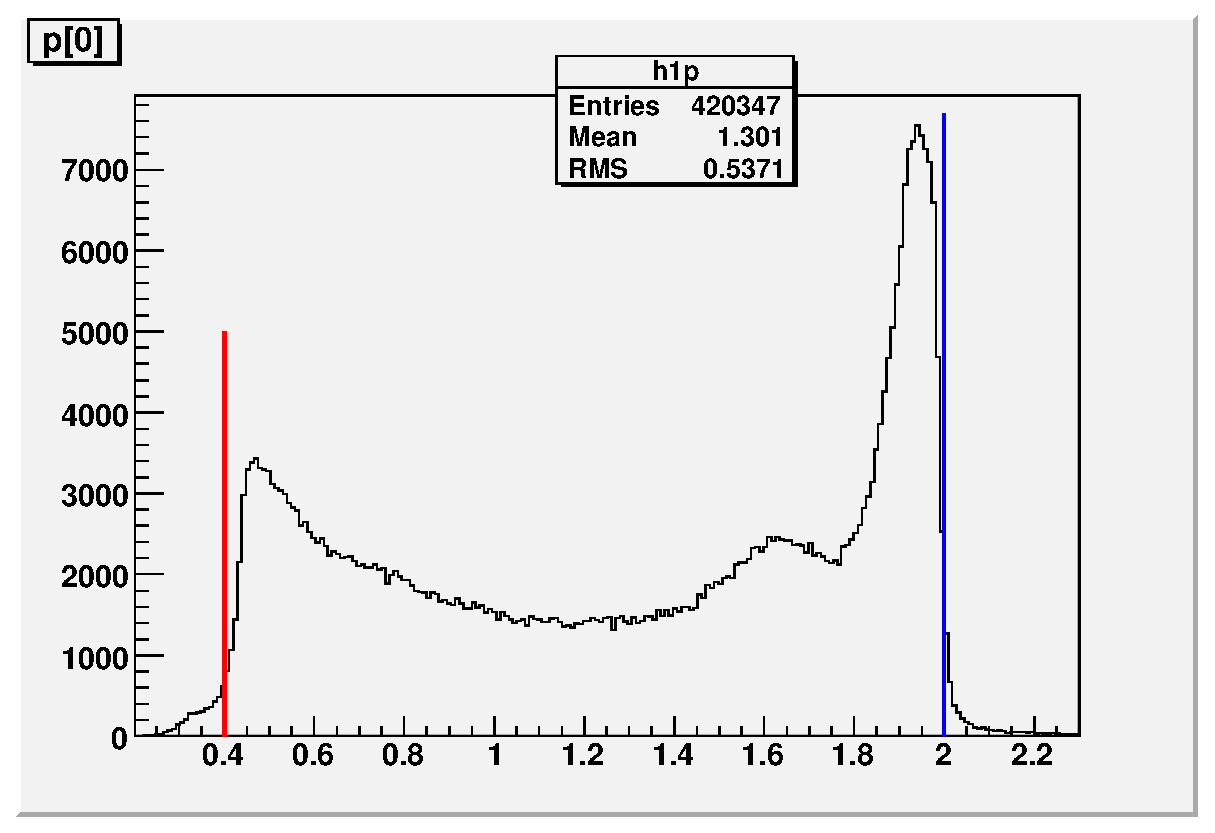
\includegraphics[width=0.8\textwidth]{TexmakerMyFinTh/chap4simul/FigCuts/pMinCtFrmRtPrmptEb2.eps}  %0.6 is the fraction of the real image width????
\leavevmode 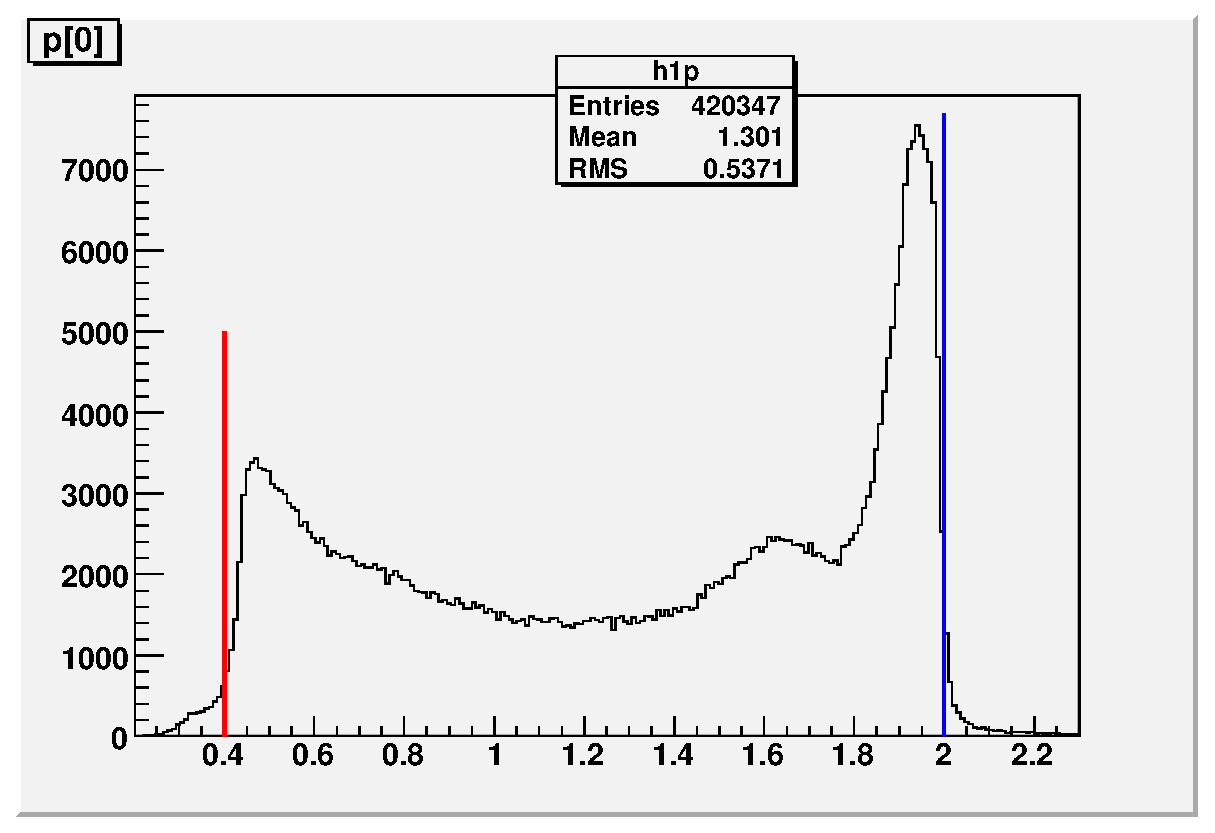
\includegraphics[width=0.8\textwidth]{TexmakerMyFinTh/chap4simul/FigCuts/pMinCtFrmRtPrmptEb2}  %0.6 is the fraction of the real image width????
\caption[Maximum and minimum momentum cuts]{The maximumum and minimum momentum cuts (on 2.0 GeV \nd3 data).
%\textcolor{red}{SEK: Memo to self: in the future use 0.45 GeV.}
}
\label{pMnMxCt}
\end{figure}

\subsection{Vertex-Z cuts}
\label{vzCuts}

In the EG4 experiment, the ND$_3$ polarized target was of 1 cm long and was placed at (x= 0, y = 0, z = -100.93 cm) in the CLAS coordinate system. Since the beam electrons have to go through a few foils %materials 
before reaching the target as well as the detector, 
we want to reject electron tracks with vertices 
%sometimes, many of the electrons that get detected happen to have scattered from points (scattering centers) that are outside the target volume. Our focus being on events that scattered off the actual target material, we want to reject those electrons that had %its 
%reconstructed vertices 
outside the target volume. %To do just that we 
For this purpose, use a cut on the reconstructed vertex co-ordinate ``v$_z$''. %But, because the resolution of ``v$_z$'' or any of the other variables is not good enough to cut events right at the edges of the target volum. Rather, the actual resolution
However the vertex resolution demands reasonably %much 
wide ``v$_z$'' cuts so as not to lose too many %much of 
good events. % due to the cuts applied. 
That is why the distribution of ``v$_z$'' was %is 
studied and based on the position and width of the distribution as well as our knowledge of the location of various foils and target materials, the cuts on ``v$_z$'' were decided. %Obviously, we were initially tempted to have a simpler, single set of cuts for all the kinematics (such as $\pm$ 4 or 5 cm on both sides of the nominal target  position), but it 
It was seen (see Figs. \ref{vzCtExp} and \ref{vzCtSim}) that the resolutions get worse and the distributions get wider as we go to lower \qsqs values, so again \qsqs dependent cuts were chosen for both data and simulation with the cuts tightening as \qsq increases.

\begin{figure}[H]%[htp] %ht, htpb (p - float, b = bottom, h=? t = top)
\centering
%\leavevmode 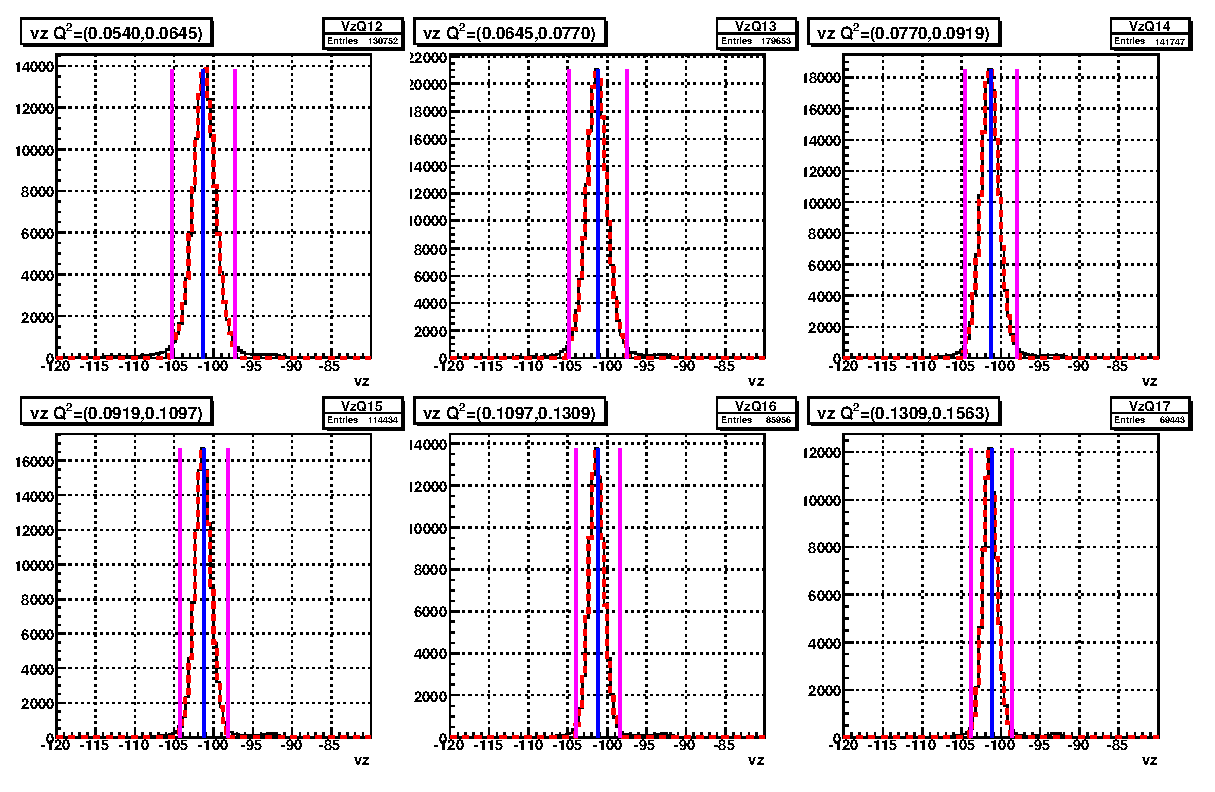
\includegraphics[width=1.0\textwidth]{TexmakerMyFinTh/chap4simul/FigCuts/vzCutsFinalEb2.eps}  %0.6 is the fraction of the real image width????
\leavevmode \includegraphics[width=1.0\textwidth]{TexmakerMyFinTh/chap4simul/FigCuts/vzCutsFinalEb2Ncropped}  %0.6 is the fraction of the real image width????
\caption[v$_z$ cuts (Exp.)]{2.0 GeV data showing the \qsqs dependent v$_z$-cuts (the magenta lines on the left and right of the peaks) in some of the \qsqs bins. The continuous black line represents events before applying all the other event selection cuts (except on v$_z$) and the thicker dotted red line are the events after the cuts. The blue lines are the centers of the distributions, from which the cuts are 3 times $\sigma$ away on each side, where $\sigma$ is the standard deviation for the distribution in the given \qsqs bin (both the central value and the $\sigma$ are determined during the cut development studies).}
\label{vzCtExp}
\end{figure}

As in the case of EC variables, the reconstructed ``v$_z$'' distribution in the simulation does not come out quite the same as in the experimental data %(see the separate section discussing the various issues encountered in simulation). Despite our tremendous efforts, intended agreement in the distributions could not be achieved and to 
. To have the same fraction of events in the corresponding \qsqs bins as in the experimental data, a separate set of cuts (determined based on the distributions of both types of data) had to be used for simulation. For this purpose, the Gaussian fit parameters $\mu$ and $\sigma$ (representing the mean and standard deviation) for all the \qsqs bins were tabulated separately for both data and simulation and separate sets of $\pm 3\sigma$ cuts were determined for all bins. For example, if $\mu_q$ and $\sigma_q$ were the two Gaussian fit parameters for the $q^{th}$ \qsqs bin of either data or simulation, then the lower and upper cuts for ``v$_z$'' for that data set in the given \qsqs bin would be $\mu_q - 3\sigma_q$ and $\mu_q + 3\sigma_q$ respectively (as shown by the magenta vertical lines in Figs. \ref{vzCtExp} and \ref{vzCtSim}.

%\textcolor{red}{My Original Question here was: Should I list all other cuts in a table (may go to Appendix)??}\\
%\textcolor{blue}{You wrote: ``Not sure what you mean''}\\
%\textcolor{red}{Because I showed these \qsq-dependent cuts for only 6 \qsqs bins (in figures), I was wondering if I should list the cuts for other bins in a table somewhere. I guess, may be not.}



\begin{figure}[H]%[h] %ht, htpb (p - float, b = bottom, h=? t = top)
%\leavevmode 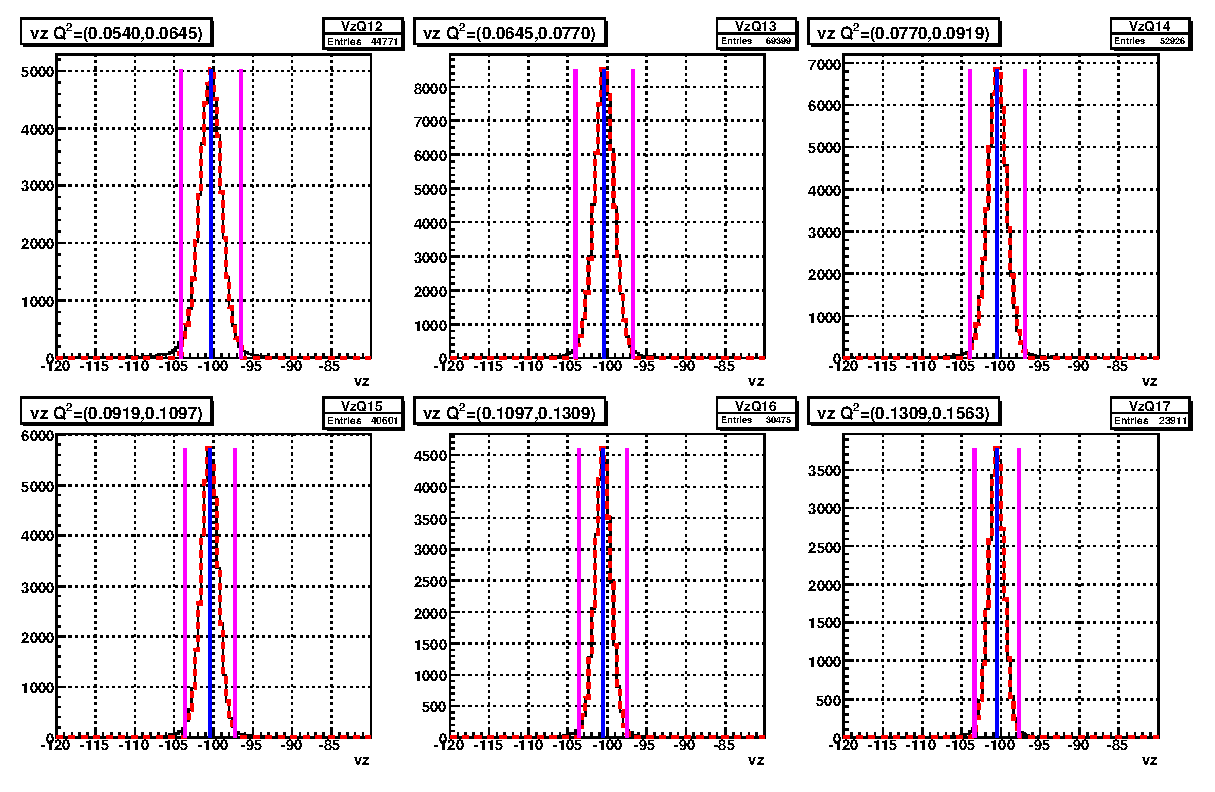
\includegraphics[width=1.0\textwidth]{TexmakerMyFinTh/chap4simul/FigCuts/vzCutsFinalEb2sim.eps}  %0.6 is the fraction of the real image width????
\leavevmode \includegraphics[width=1.0\textwidth]{TexmakerMyFinTh/chap4simul/FigCuts/vzCutsFinalEb2simNcropped}  %0.6 is the fraction of the real image width????
\caption[v$_z$ cuts (Sim.)]{\qsqs dependent v$_z$-cuts on simulation data (similar to Fig. \ref{vzCtExp}).}
\label{vzCtSim}
\end{figure}



%\section{Radiative Corrections}
%Plgiarism Warning: (paraphrasing not done.)
%GSIM - the CLAS Monte Carlo simulation program using GEANT 3.21 libraries from CERN -implements a complete. \cite{clasBrooks}%pg 31 

\subsection{Fiducial Cuts}
\label{fidCuts}

Similar to the cuts discussed so far, we also had to match the region of good efficiency of the physical detector with the corresponding region from the simulation. For the experimental and simulation data to be comparable, they must have the same detector acceptance. %, otherwise systematic uncertainty is introduced into the calculations. 
Two event variables polar angle (\thvtx) measured at the vertex and the azimuthal angle $\phi_{DC1}$ measured at the drift chamber layer 1 are chosen to define the good efficiency regions of the detector. The reason for the choice of the variable \thvtx~ should be obvious because it is directly related with the kinematic variables \qsqs and $W$ used in the analysis. However, due to the momentum dependent rotational effect of the magnetic field on the reconstructed azimuthal angle (\phvtx) at the vertex, the angle $\phi_{DC1}$ is preferred over \phvtx~ to define the fiducial region because that allows the easy selection (rejection) of the events which passed through and got detected by the more (less) reliable central (marginal) regions of the Cerenkov Counters. %drift chambers. %kp: 12/6/13 after SEK insistence
After a careful and extensive study of the event distributions on both data and simulation, we arrived at four sets of fiducial cuts in terms of the variables \thvtx, $\phi_{DC1}$ and the torus current normalized inverse momentum i.e., \invP.%I$_{torus}$/2250p.% This cut allowed the maximum possible inclusion of the high efficiency regions of

%
% Pass2 fiducial cuts: all defined in #include "/home/adhikari/LinkedFiles/fiducialCutsPass2.h"   
% The final results were for array indices C71 and S181
% The fiducial cuts used for C71_S181 were
%   
%
%   fidCtV1 
%   fidCtExpBySimAndEConlyInInvPvsThVtx
%   fidMoreMIPB
%
% %%%%%%%%%%%%%%%%  
%
%  where,
%   fidCtV1: if(fidCtExp2Sim==true && fidCtReg2EC==true) fidCtV1 = true;
%       with
%  bool fidCtReg2EC = Pass2FidCutLatestFromRegECcomparison(Ebi, p[0], thDc1PosRad);//now in the same fiducialCutsPass2.h file
%     corresponding image: 
%           https://www.jlab.org/Hall-B//secure/eg4/adhikari/Analysis/Pass2/Cuts/Fid/BkUp/invMomVsThDc1Pass2Ebi4Ratio.gif
%
%  bool fidCtExp2Sim = Pass2FidCutLatest(phDc1PosRad, thetaRadC); //now in the same fiducialCutsPass2.h file
%    corresponding image:
%          https://www.jlab.org/Hall-B//secure/eg4/adhikari/Analysis/Pass2/Cuts/Fid/fidCutPlotsSet2_Eb2_RatioBigger.gif 
%          &.../fidCutPlotsSet2_Eb1_Ratio.gif
%
%   
%
%   fidCtExpBySimAndEConlyInInvPvsThVtx = Pass2FidCutOnInvPvsThVtx(Ebi, ppC, thetaRadC);//3/8/16 defined in commonItems4SimExp.h for now
%              ~/secure/Analysis/Pass2/Cuts/Fid/invMomVsThVtxPass2Ebi1RatioRegByEConlyFidCut09.gif
%
%  if(Ebi==2) fidMoreMIPB = moreFidCutsWithMoreInvPBins(Ebi, ppC, phDc1DegPlusMinus30, thVtxDeg);//7/11/16 defined in moreFidCuts.h
%  else if(Ebi==1) fidMoreMIPB = moreFidCutsWithMoreInvPBinsEbi1(Ebi, ppC, phDc1DegPlusMinus30, thVtxDeg);//7/18/16 defined in moreFidCuts.h
%   for which see plots:
%       //https://www.jlab.org/Hall-B//secure/eg4/adhikari/Analysis/Pass2/Cuts/Fid/MoreCts/moreFiducialCutsMoreInversePBinsEbi1.gif
%       and moreFiducialCutsMoreInversePBinsEbi2.gif   //11/13/16
%   




% See EG4 update (Glasgow, by S.E. Kuhn) and make eps plots like those included
% include the DC shadow & granularity  figures, (may be in a separate section on Simulation/GSIM issues and refer to it from this section)

% include the Regular/EC-only 2D plots to show the CC-inefficient regions (to be discarded by some of the angular cuts)
% Show the discrepancy plots in theta and v$_z$ in data and simulation (for a few q2 bins)
%After a laborious work on getting simulation match with the data to a reasonably good degree, we did a final comparison work to determine the fiducial cuts. We obtained overlays of one-dimensional histograms of different variables, and also studied the ratios both in one and two dimensions. Based on these comparisons, regions of relatively bad matching were singled out and cuts were developed to reject such parts of the kinematic space.\textbf{\textcolor{red}{to be be elaborated more ..}}


The first set (see Fig. \ref{figFidRegVsEC1}) of fiducial cuts  were determined by comparing regular and EC-only data (which were taken using triggers that didn't involve CC) and selecting cuts such that regions with relatively darker spots (reflecting very low CC-efficiency) were rejected.

\begin{figure}[H]%[h] %ht, htpb (p - float, b = bottom, h=? t = top)
\centering
%\leavevmode \includegraphics[width=0.9\textwidth]{TexmakerMyFinTh/chap4simul/FigCuts/phDc1PosVsThv_inInvPbins_ExpEb2WdOsiNphNoThCts4Ths.eps} 
%\leavevmode \includegraphics[width=0.9\textwidth]{TexmakerMyFinTh/chap4simul/FigCuts/phDc1PosVsThv_inInvPbins_ExpEb2WdOsiNphNoThCts4Ths} 
%\leavevmode \includegraphics[width=0.9\textwidth]{figuresEG4/NewP2/FidCuts/invMomVsThDc1Pass2Ebi4Ratio.png}
%\leavevmode \includegraphics[width=0.9\textwidth]{figuresEG4/NewP2/FidCuts/invMomVsThDc1Pass2Ebi4RatioCropped.png}
%\caption[Fiducial cuts]{Fiducial cuts determined by comparing the distributions of regular and EC-only {\bf experimental data} as a function of \invP and $\theta_{DC1}$. %Here in the top panels, we see distributions of regular and EC-only data respectively and in the bottom panel we have the ratios of the two 
\leavevmode \includegraphics[width=1.0\textwidth]{figuresEG4/NewP2/FidCuts/invMomVsThVtxPass2Ebi4RatioCropped.png}
\caption[Fiducial cuts]{Fiducial cuts determined by comparing the distributions of regular and EC-only {\bf experimental data} as a function of \invP and $\theta_{vtx}$. %Here in the top panels, we see distributions of regular and EC-only data respectively and in the bottom panel we have the ratios of the two 
Here in the top panels, we see distributions of ratios of the regular and EC-only data respectively in linear and log scales in the color axis respectively. Inefficient regions of the CC are excluded using the indicated cuts.} %Fiducial cuts
\label{figFidRegVsEC1}
\end{figure}

The second set of cuts came from a similar comparison between the regular and EC-only data in the \invP vs \thvtx (instead of $\theta_{DC1}$) space (see Fig. \ref{figFidRegVsEC2}) .

\begin{figure}[H]%[h] %ht, htpb (p - float, b = bottom, h=? t = top)
\centering
%\leavevmode \includegraphics[width=0.9\textwidth]{TexmakerMyFinTh/chap4simul/FigCuts/phDc1PosVsThv_inInvPbins_ExpEb2WdOsiNphNoThCts4Ths.eps} 
%\leavevmode \includegraphics[width=0.9\textwidth]{TexmakerMyFinTh/chap4simul/FigCuts/phDc1PosVsThv_inInvPbins_ExpEb2WdOsiNphNoThCts4Ths} 
%\leavevmode \includegraphics[width=0.9\textwidth]{figuresEG4/NewP2/FidCuts/invMomVsThVtxPass2Ebi1RatioRegByEConlyFidCut09.png}
\leavevmode \includegraphics[width=0.9\textwidth]{figuresEG4/NewP2/FidCuts/invMomVsThVtxPass2Ebi1RatioRegByEConlyFidCut09cropped.png}
\caption[Fiducial cuts]{Fiducial cuts determined by comparing the distributions of regular and EC-only {\bf experimental data} as a function of \invP and vertex angle \thvtx. Here, the vertical cut near \thvtx=25 degrees is to avoid the region of low efficiency possibly due to %some dead wires
  dead wires in DC.} %Fiducial cuts
\label{figFidRegVsEC2}
\end{figure}



The third set of cuts came from a %somewhat similar
comparison %but this time 
between the experimental and the corresponding simulated data as shown in the Fig. \ref{figFidExpVsSim}. 
%The ratio of their distributions in a two dimensional space defined in terms of two variables \thvtx and the torus current normalized inverse momentum (i.e. $ I_{torus}/(2250 p)$. In one case, the ratio was taken between the regular experimental data and the "EC-only" experimental data (with CC-signal not required in the event trigger) (see Fig. \ref{figRegByEConly}) and in the other case, the ratio was of the experimental deuteron data (after background subtraction) to the simulated deuteron data (see Fig. \ref{figangCts2}). From these comparisons, some of the regions that showed big CC-inefficiencies or big discrepancies between data and simulation were selected and removed from the fiducial region %defined in terms of some more cuts 
as indicated by various straight lines in the two plots.



\begin{figure}[H]%[h] %ht, htpb (p - float, b = bottom, h=? t = top)
\centering
%\leavevmode \includegraphics[width=0.9\textwidth]{TexmakerMyFinTh/chap4simul/FigCuts/phDc1PosVsThv_inInvPbins_ExpEb2WdOsiNphNoThCts4Ths.eps} 
%\leavevmode \includegraphics[width=0.9\textwidth]{TexmakerMyFinTh/chap4simul/FigCuts/phDc1PosVsThv_inInvPbins_ExpEb2WdOsiNphNoThCts4Ths} 
%\leavevmode \includegraphics[width=0.98\textwidth]{figuresEG4/NewP2/FidCuts/fidCutPlotsSet2_Eb2_RatioBigger.png}
\leavevmode \includegraphics[width=0.98\textwidth]{figuresEG4/NewP2/FidCuts/fidCutPlotsSet2_Eb2_RatioBiggerCroppedIpBins0n1.png}
\caption[Fiducial cuts ]{Distribution (in two of six bins of $I_{torus}/(2250 p)$) of %{\bf experimental} and {\bf simulated} data ( for 2.0 GeV) and their ratios 
ratios of {\bf experimental} and {\bf simulated} data ( for 2.0 GeV) (both in linear and log-z scales) as a function of vertex angle $\theta_{vtx}$ and azimuthal angle $\phi_{DC1}$ as measured by the track position at the first drift chamber layer (angles in degrees). The dotted lines indicate the fiducial cuts for accepting good electrons. %\textcolor{red}{SEK: Do you have the analogous plot for simulation? Include \\ Make magenta lines thicker. } %Comment out eventually
} %Fiducial cuts}
\label{figFidExpVsSim}
\end{figure}


%> 1) Fiducial cuts (Very short)   %Dr. Kuhn's comment on Jlab email dated November 3, 2013 3:45 pm  (title Re: "Complete" Thesis)
%
%p. 116: We used the polar angle at the vertex NOT because it isn't affected by the target magnetic field (it most certainly is), but because the acceptance is defined by the range in scattering angle (as you showed earlier, dOm = sintheta dtheta dphi). For the same reason, we SHOULD have chosen phi at the vertex, as well; however, since the effect of the target field on phi is just a constant offset (rotation around the z-axis), the range phi_max - phi_min is the same at DC1 as at the vertex, giving the same acceptance. We chose DC1 because that's what actually limits the phi acceptance. As you understand, this section is not yet complete. You need to explain that we use the amount of bending (Itor/p*2250) as a 3rd variable, since E'=p is the third variable the determines the acceptance, but the amount of bending has direct correlation to where on the CC a track ends (i.e., the phi range). (You should move the corresponding explanation of ip up from p.122).                      You should also show a couple more plots with different Itor/p*2250 as well as a couple of plots for the simulation to convince the reader that our choices are robust.                   Figs. 51a and 51b should be given a full width each since they have a lot of information and are hard to read otherwise (make them two different figures). I also am confused about your explanation for Fig. 51a):                  I seem to remember that we divided ND3 for standard trigger by ND3 for EC only trigger;  dividing ND3 data by D simulation seems to make little sense. Please check!

Lastly, further sets of cuts were developed based on the distribution of the average number of photo electrons (nphe) as recorded by the Cerenkov Counter (CC) (see Fig. \ref{figFidAvgNph1}).

\begin{comment}
\begin{figure}[H]%[h] %ht, htpb (p - float, b = bottom, h=? t = top)
\centering
\leavevmode \includegraphics[width=1.1\textwidth]{figuresEG4/NewP2/FidCuts/moreFiducialCutsMoreInversePBinsEbi2.png}
\caption[Fiducial cuts ]{}
\label{figFidAvgNph}
\end{figure}
\end{comment}


\begin{figure}[H]%[h] %ht, htpb (p - float, b = bottom, h=? t = top)
\centering
%\leavevmode \includegraphics[width=1.1\textwidth]{figuresEG4/NewP2/FidCuts/moreFiducialCutsMoreInversePBinsEbi2first4Bins.png}
\leavevmode \includegraphics[width=1.1\textwidth]{figuresEG4/NewP2/FidCuts/moreFiducialCutsMoreInversePBinsEbi2first4BinsN.png}
\caption[Fiducial cuts (first 4 bins)]{Average Nphe distributions as a function of $\phi_{DC1}$ (along Y-axis) and $\theta_{vtx}$ (along X-axis) in first four bins of $\frac{I_{tor}}{p \cdot 2250}$. The black lines show the cuts that reject the very low CC-inefficiency regions.}
\label{figFidAvgNph1}
\end{figure}


\begin{figure}[H]%[h] %ht, htpb (p - float, b = bottom, h=? t = top)
\centering
\leavevmode \includegraphics[width=1.1\textwidth]{figuresEG4/NewP2/FidCuts/moreFiducialCutsMoreInversePBinsEbi2next4Bins.png}
\caption[Fiducial cuts (next 4 bins)]{Average Nphe distributions as a function of $\phi_{DC1}$ (along Y-axis) and $\theta_{vtx}$ (along X-axis) in next four bins of $\frac{I_{tor}}{p \cdot 2250}$. The black lines show the cuts that reject the very low CC-inefficiency regions.}
\label{figFidAvgNph1}
\end{figure}


\begin{figure}[H]%[h] %ht, htpb (p - float, b = bottom, h=? t = top)
\centering
%\leavevmode \includegraphics[width=1.1\textwidth]{figuresEG4/NewP2/FidCuts/moreFiducialCutsMoreInversePBinsEbi2last4BinsN.png}
\leavevmode \includegraphics[width=1.1\textwidth]{figuresEG4/NewP2/FidCuts/moreFiducialCutsMoreInversePBinsEbi2last4BinsN.png}
\caption[Fiducial cuts (last 4 bins)]{Average Nphe  distributions as a function of $\phi_{DC1}$ (along Y-axis) and $\theta_{vtx}$ (along X-axis) in last four bins of $\frac{I_{tor}}{p \cdot 2250}$. The black lines show the cuts that reject the very low CC-inefficiency regions.}
\label{figFidAvgNph1}
\end{figure}


%%%%%% To be worked 
%%%%%% To be worked 
%%%%%% To be worked 
%%%%%% To be worked 
%%%%%% To be worked 



\clearpage




%\begin{comment}
\section{Data Quality and Stability Checks}
%\textbf{\textcolor{red}{Yet to be fleshed out.}}
With an available set of good  event/electron selection cuts, beam charge (measured by Faraday cup) normalized total event counts (sometimes also known as event ``yield''), as well as polarization dependent %polarized count 
differences, were calculated for each of the data files for all the runs %run numbers 
and then plotted against the run number to study the data quality and stability as shown by Figs. \ref{figyldTot}, \ref{figyldDiff} and \ref{figrstADCs}.

If nothing unusual happened or if the experimental conditions are not changed, %between the data taking, 
then it is expected that the event yield as well as the count differences remain constant over time. Therefore, the graphs of these event counts plotted versus time or run number (which also roughly reflect the flow of time) should indicate the stability and quality of the data collected. For example, Fig. \ref{figyldTot} shows such a total yield plot for all the data files from the 2.0 GeV beam energy data set on deuteron target. We can see that these data runs display %quite 
 some features of instability over the full period of time, but %some degree of SEK
 stability over short time periods. For example, all the data with run numbers below about 51610 show significantly higher event yield than the runs after that run %. This could have been due to  and it suddenly drops after around that run number 
 (possibly due to  beam-target misalignment %that could have happened due to target replacement activity).
 as indicated by raster magnet ADC values in Fig \ref{figrstADCs}. 



Likewise, the stability of the polarized %total %GED
count differences in the elastic region ($0.9$ GeV $<W<1.0$ GeV) as well as separately in the delta ($\Delta$) resonance region were studied by plotting them versus the same run numbers (here the elastic and $\Delta$-resonance regions are %should be 
considered separately, because the spin asymmetries in these two regions have opposite signs, which would 
%otherwise cancel each other's effects in the total count difference. %, thus not allowing us any instability to be seen if they existed). 
have decreased the observed difference if combined.
To further enhance the sensitivity of the observation, the difference of the count differences measured in the elastic and $\Delta$-resonance regions as given by 

\begin{eqnarray}
\label{eqPolED}
\Delta N_{elastic} - \Delta N_{\Delta-res} = \frac{1}{P_b P_t} \left[ \left( \frac{N^+}{FC^+} - \frac{N^-}{FC^-} \right)_{elastic} -   \left( \frac{N^+}{FC^+} - \frac{N^-}{FC^-} \right)_{\Delta} ~ \right]
\end{eqnarray}
were plotted (see Fig. \ref{figyldDiff}). It was observed %, to our delight, 
that this elastic normalized count difference (which is what really matters to our analysis, in the end) was much more stable than the total yield.

%http://amath.colorado.edu/documentation/LaTeX/reference/figures.html
\begin{figure} [H] %[h] %ht, htpb (p - float, b = bottom, h=? t = top)
%\leavevmode \includegraphics[width=0.6\textwidth]{chap6expSetup/Figures/cebaf.eps}  %0.6 is the fraction of the real image width????
  %\leavevmode \includegraphics[width=0.9\textwidth]{FigQualCheckBkGrnd/totYld_2_2.eps}  %0.6 is the fraction of the real image width????
  \leavevmode \includegraphics[width=0.9\textwidth]{TexmakerMyFinTh/FigQualCheckBkGrnd/totYld_2_2.png}  %0.6 is the fraction of the real image width????
  \caption[Normalized total yield (2.0 GeV (ND$_3$))]{Total normalized yield ($= \frac{N^+ + N^-}{FC^+ + FC^-}$) for 2.0 GeV ND$_3$ runs.}
  \label{figyldTot}
\end{figure}



\begin{figure}[H] %[h] %ht, htpb (p - float, b = bottom, h=? t = top)
  %\leavevmode \includegraphics[width=0.9\textwidth]{FigQualCheckBkGrnd/yldDiffnormED_2_2.eps} 
  \leavevmode \includegraphics[width=0.9\textwidth]{TexmakerMyFinTh/FigQualCheckBkGrnd/yldDiffnormED_2_2.png} 
  \caption[$\Delta N$ for elastic minus $\Delta$-resonance]{Polarized yield differences (Eq. \ref{eqPolED}) normalized with $P_bP_t$ and BPM/F-cup for elastic peak minus that for the $\Delta$ peak for the 2.0 GeV \nd3 runs.}
  \label{figyldDiff}
\end{figure}

The same was also repeated for the other variables such as the root-mean-square of the ADC values (see Fig. \ref{figrstADCs}) which carry information on the X and Y coordinates of the beam at the interaction vertex, thus their plots giving us somewhat more direct information on whether there was any misalignment between the beam and the target.

\begin{figure}%[h] %ht, htpb (p - float, b = bottom, h=? t = top)
  %\leavevmode \includegraphics[width=1.0\textwidth]{FigQualCheckBkGrnd/rmsRastAdcVRun2_2.eps} 
  \leavevmode \includegraphics[width=1.0\textwidth]{TexmakerMyFinTh/FigQualCheckBkGrnd/rmsRastAdcVRun2_2.png} 
  \caption[RMS of raster ADCs]{Root-mean-square of the ADC values for the raster magnet currents in the directions %arms 
  X and Y. The distributions show a larger raster size in the y-direction for the first group of runs, indicating that the beam may have been hitting the edges and the walls of the target or other more dense structure support materials, thus explaining the higher total yield for the corresponding runs as shown by the Fig. \ref{figyldTot}. This does not affect our final analysis because these off-target materials are not polarized and, hence, do not contribute to the polarization dependent count difference ($\Delta N$) used in the final analysis.}
  \label{figrstADCs}
\end{figure}

Based on the  studies of these quality and stability plots, the data runs were divided into subgroups with each beam energy data set. In each subgroup, the data showed more stability than over the whole run period for the given beam energy. For example, in case of the 2.0 GeV deuteron data, the runs were divided into four distinct sub groups corresponding to the four separate bands as seen in the Fig. \ref{figyldTot}. These subgroups were later treated and analyzed separately to get the corresponding normalized polarized count differences (with all data runs from each subgroup combined together). After the initial combination within the subgroups, they were again combined into the grand total by properly considering the half-wave-plate status, and the target polarization directions.

%\end{comment}



\begin{comment} %Already commented (on my thesis version)
%\usepackage{verbatim} % For multiline comments: http://www.devdaily.com/blog/post/latex/multi-line-comments-in-latex-begin-123-comment-125-verbatim
\kpb
  Figures (fig~(\ref{figTRvI_ls})) and (fig~(\ref{figYldvTR_l}))
% http://texblog.wordpress.com/2007/08/01/placing-figurestables-side-by-side-minipage/
\begin{figure}[ht]
\begin{minipage}[b]{0.5\linewidth}
\centering
\includegraphics[scale=0.4]{FigQualCheckBkGrnd/trRateVIb_lumScanRuns.eps}
%\caption{default}
 \caption[Trigger rate]{Trigger rate versus beam current for 1.3 GeV luminosity-scan runs (6 runs) showing that the rate is proportional to the current or luminosity general.}
\label{figTRvI_ls}
\end{minipage}
\hspace{0.5cm}
\begin{minipage}[b]{0.5\linewidth}
\centering
\includegraphics[scale=0.4]{FigQualCheckBkGrnd/yldVtrRateTh0_lumScanRuns.eps}
  \caption[Yield of 1.3 GeV luminosity scans]{Normalized yield vs the trigger rate for the 1.3 GeV luminosity-scan runs (6 runs) showing that the detection efficiency decreases with the rate at which the events occur (i.e., the trigger rate or effectively the luminosity).}
%\caption{default}
\label{figYldvTR_ls}
\end{minipage}
\end{figure}
\kpe




\begin{figure}
\centering
%The following \mbox{} gives the overfull \hbox warning
\mbox{\subfigure{\includegraphics[width=3in]{FigQualCheckBkGrnd/trRateVIb_lumScanRuns.eps}}\quad
\subfigure{\includegraphics[width=3in]{FigQualCheckBkGrnd/yldVtrRateTh0_lumScanRuns.eps} }}
\caption[Trigger Rate]{( \textbf{Left}: Trigger rate versus beam current for 1.3 GeV luminosity-scan runs (6 runs) showing that the rate is proportional to the current or luminosity. \textbf{Right}: Normalized yield vs the trigger rate for the 1.3 GeV luminosity-scan runs (6 runs) showing that the detection efficiency decreases with the rate at which the events occur (i.e., the trigger rate or effectively the luminosity).} 
\label{figlsPlts}
\end{figure}

%Note that for JPEG images the graphics package is required: \usepackage{graphics}

\begin{figure}[htpb] %ht, htpb (p - float, b = bottom, h=? t = top)
  \leavevmode \includegraphics[width=1.0\textwidth]{FigQualCheckBkGrnd/yldVtrRateTh0_2_2.eps} 
  \caption[Yield vs Trigger Rate]{Normalized yield vs the trigger rate within 6-10$^o$ of $\theta$ for the first of the three sets of 2.3 GeV \nd3 runs showing the drop of detection efficiency with the trigger rate.}
  \label{figYldvTR_22}
\end{figure}



\begin{figure}[htpb] %ht, htpb (p - float, b = bottom, h=? t = top)
  %\leavevmode \includegraphics[width=1.0\textwidth]{FigQualCheckBkGrnd/Eff_vs_Lumi_EG4.eps} %For some reason this email-downloaded-copy didn't work 
  %Looks like that is a acrobat-reader problem
  \leavevmode \includegraphics[width=1.0\textwidth]{FigQualCheckBkGrnd/Eff_vs_Lumi_EG4convert.eps} 
  \caption[Fit parameter ratios vs Bin Numbers]{Ratio of fit parameters (slope/offset) plotted against the three bin numbers, where the parameters are from the various linear fits to the normalized yields vs trigger rates such as . The average of the 7 ``good'' curves (black) can be used to correct data and the ``error bars'' (the 1-sigma deviation) as a systematic error.(Plot courtesy of S. Kuhn).}
  \label{figpRatioVthBin}
\end{figure}

\end{comment}  %Already commented (on my thesis version)

%\end{comment} 



%\chapter{Kinematic Corrections}
\section{Kinematic Corrections}
\label{cha:KineCor}
The reconstructed event vertices and associated particle 4-momenta are slightly off from their true values for several reasons. First, % of all, %SEK
RECSIS does not take into account the fact that the beam is rastered in polarized target experiments. Next, any 
imperfections and mis-alignments of detectors and other components of the experimental set-up are not accounted for. 
Furthermore, the torus field map is not known precisely. 
In addition, the effects of multiple-scattering and particle energy losses are not considered in RECSIS. %Finally, RECSIS itself has imperfections inherent in its algorithm. %SEK: Unless you want to explain, leave out.
Therefore, to get more accurate results from the data analysis, the data quality must be improved by applying various kinematic corrections. Following is the list of the corrections that were applied for %is applied for each particle from our data 
the analysis:

\begin{enumerate}
\item Incoming (beam) energy loss correction (due to ionization) 
\item Tracking corrections
%%%%\begin{enumerate}
%%%%\item Beam off-set correction % equivalent to Raster correction?
%\item Drift chamber dependent momentum correction
%\item Z-vertex correction
%%%%\item Solenoid axis tilt correction
%%%%\item Solenoid axis offset correction
%%%%\end{enumerate}
%\item Stray magnetic field correction 
\item Drift chamber dependent momentum correction
%\item Multiple scattering correction (Not considered because, we are looking at electron-only inclusive events)
\item Outgoing energy loss correction (due to ionization after scattering) %/reaction))
\end{enumerate}



%\section{Incoming Energy Loss Correction}
\subsection{Incoming Energy Loss Correction}
%Out of these corrections, the first one
The first correction listed above considers the loss of beam energy due to atomic collisions before the actual nuclear scattering takes place. %As an adjustment for the loss, an estimate of 2 MeV
A good estimate for this loss is 2 MeV on average \cite{pComKuhn, pComBosted}, which is subtracted from the nominal beam energy. This correction is applied during the analysis whenever the beam energy is involved\footnote{The beam energies that we used were derived from the Hall A and Hall C Tiefenback energies  or the MDSY1c or MDSY3c energies\cite{eg4Ebeam}}, %For more info, read X. Zheng's analysis note around page 35.
and therefore it is not included in the correction package described below.





%\section{Raster Correction}

%This section still being expanded ... \newline \newline

%\subsubsection{Beam Rastering in Hall-B Polarized target Experiments}


The polarized electron beam coming from CEBAF to Hall B is rastered in polarized target experiments. This 
is done to minimize radiation damage (depolarizing effects) to the polarized target and also to make maximum use of 
the target material (effective beam size increases and, therefore, the overall volume of exposed target increases). 
The beam is periodically spiraled covering a circular region of the target cross-section by using two raster 
magnets - one for the horizontal (X) direction and the other for the vertical direction (Y). The currents driving 
the two magnets are continuously recorded by analog-to-digital converters (ADCs).

\begin{figure}[htpb] %ht, htpb (p - float, b = bottom, h=? t = top)
\centerline{\epsfig{height=10cm,width=15cm,file=figuresEG4/FigKineCor/Raster_Corr_Formulae_Page_1.png}}
\caption{Raster correction geometry illustration (Figure courtesy of S. Kuhn)}
\label{fig:RstGeoKuhn1}
\end{figure}

The ADC values thus recorded can be translated to the coordinates (x,y) of the exact beam position at the target. The values of x,y can then be used to make corrections to the original track by RECSIS (which assumes x and y were zero), allowing better z-vertex and azimuthal angle ($\phi$) reconstruction. The better z-vertex reconstruction allows better selection of events from the target proper, rejecting events from upstream and downstream %up-beam and down-beam %GED
windows (especially for particles at small angles), and can also be used to reduce accidental coincidences in multi-particle final states (or to look for offset decays such as from $\Lambda$). Correction of $\phi$ improves missing mass resolution for multi-particle final states which is very important in exclusive channel analysis. In addition, plotting a two-dimensional histogram of events as a function of the raster information x and y, one can look for mis-steered beam that might have hit the target cup edges.

\begin{figure}[htpb] %ht, htpb (p - float, b = bottom, h=? t = top)
\centerline{\epsfig{height=10cm,width=15cm,file=figuresEG4/FigKineCor/Raster_Corr_Formulae_Page_2.png}}
\caption{Raster correction geometry illustration (Figure courtesy - S. Kuhn)}
\label{fig:RstGeoKuhn2}
\end{figure}

A procedure was developed by P. Bosted \etal \cite{rstcor_cn} to translate the raster ADC values %counts 
into the beam coordinates x, y and then use them to improve the z-vertex and $\phi$ reconstruction. This procedure was successfully applied in previous CLAS experiments and EG4 has also embraced it to do the needed raster correction.


In short, the procedure for this correction is as follows: %does the following:
\begin{enumerate}
\item Translates raster-ADC values to beam coordinates x and y.
\item Corrects the event vertex z-coordinate (represented as v$_z$ in the data). %pass1 ntuples) %SEK
\item Corrects the azimuthal angle $\phi$ of each particle in the event.
\end{enumerate} 

% new paragraph \\
This correction is applied before the momentum correction. So, the partially corrected $\phi$ and v$_z$ will be a part 
of the input fed into the next stage of the kinematic correction which, henceforth, will be termed ``momentum correction''.



%\subsection{Procedure to translate ADC counts to beam positions x and y (in centimeters)}
\subsubsection{Procedure to translate ADCs to centimeters}

\begin{figure}[htpb] %ht, htpb (p - float, b = bottom, h=? t = top)
\centerline{\epsfig{height=10cm,width=10cm,file=figuresEG4/FigKineCor/Rst21pCorXY.png}}  %kp: Disabled for Suman Jee's trimming test (enable back)
%\centerline{\includegraphics[trim = 0mm 0mm 0mm 50mm, clip = true, scale = 0.5] {chap7KineCor/figures/Rst21pCorXY.png}} %7/27/12
\caption{Beam coordinates x and y calculated with the raster correction procedure.}
\label{fig:RstXY}
\end{figure}

The procedure assumes that a linear relation holds between the raster currents and the beam coordinates x and y (displacements %bendings 
in cm produced by the field of the currents) as follows:

\begin{subequations}
\label{eqRC-Adc2cm}
\begin{eqnarray}
\label{eqRC-Adc2cm1}
x = (X_{adc}-X_{offset})C_x,
\end{eqnarray}

\begin{eqnarray}
\label{eqRC-Adc2cm2}
y = (Y_{adc}-Y_{offset})C_y,
\end{eqnarray}
\end{subequations}
where, $X_{offset}$, $Y_{offset}$, $C_x$, and $C_y$ are the %constants/
parameters to be determined by the procedure. These parameters are determined by selecting reasonably well reconstructed events each consisting of more than one charged  particles tracks originating reasonably close to the nominal target center (v$_z \approx $- 101.0 cm) and using them in TMinuit (ROOT Minuit program) to minimize the $\chi^2$, defined as
\begin{eqnarray}
\label{eqRC-chiSq}
\chi^2 = \sum^N_{i=1}((z_{corr})_i - z_o)^2,
\end{eqnarray}
where $z_0$ is the 5th parameter that defines the center of the target and is to be determined from the minimization. %/fitting. 
Likewise, $z_{corr}$ is the trial value of the corrected z-vertex (a function of trial values of the first four fit parameters, as will be evident below). TMinuit will give us those values of the parameters which gives 
the $\chi^2$ a minimum value.

\begin{comment}
\begin{figure}[h] %ht, htpb (p - float, b = bottom, h=? t = top)
\centerline{\epsfig{height=15cm,width=15cm,file=figuresEG4/FigKineCor/MTc3G50916one.png}}
\caption[Vz from Empty target run]{Vertex Z-coordinates of scattered electrons from an 3.0 GeV empty-cell-target run}
\label{fig:MTcellVz1}
\end{figure}
\end{comment}

\begin{figure}[h] 
\centering
  \leavevmode \includegraphics[width=0.8\textwidth]{figuresEG4/FigKineCor/MTc3G50916one.png}   
  \caption[Vz from Empty target run]{Vertex Z-coordinates (in cm) of scattered electrons from an 3.0 GeV empty-cell-target run before (black) and after (red) the raster corrections. It is clear that the correction improves the resolution, thus revealing the positions of the empty target cells (the first two peaks near -101.0 cm) and the heat shield (around -93.0 cm).}
  \label{fig:MTcellVz1}
\end{figure}



From a simple geometry consideration (as illustrated in Figs. \ref{fig:RstGeoKuhn1} and \ref{fig:RstGeoKuhn2}), an expression for correction to the z-vertex in terms of x, y and angles of a particle track is arrived at as follows:
\begin{eqnarray}
\label{eqRC-zcor}
z_{corr} = z_{recsis} + x'/tan(\theta),
\end{eqnarray}
where $z_{recsis}$, and $z_{corr}$ are the z-vertex measured %/reconstructed 
by the tracking code and the raster-corrected z-vertex respectively, and
\begin{eqnarray}
\label{eqRC-xprime}
x' = (x~cos\phi_s + y~sin\phi_s)/cos(\phi - \phi_s),
\end{eqnarray}
is the distance in cm along the track length that was not considered in tracking (because the tracking code assumes that the track started from $x = 0$, $y = 0$); $\phi_s$ is the sector angle defined as the azimuthal angle of the sector mid-plane (equal to $(s-1 \cdot 60$ degrees, where $s$ is the sector number from 1 to 6), and $\phi$ is the azimuthal angle of the particle (in the lab-coordinate system) defined as $\phi = arctan(cy/cx)$, %atan2(cy,cx), atan2 is a programming jargon, just write "arctan" %SEK
where $cx$ and $cy$ are the x- and y- direction cosines of the track. 

Due to the difference of the actual track length (through the 50 kG magnetic field of the target) from what is assumed by the tracking software, the azimuthal angle \phs is reconstructed incorrectly. The angle \phs can now be corrected by adding a correction term $- 50 q (x'/100)/33.356/p_t$ to the reconstructed value $\phi_{recsis}$ as follows:
\begin{eqnarray}
\label{eqRC-phcor}
\phi_{corr} = \phi_{recsis} - 50 q (x'/100)/33.356/p_t,
\end{eqnarray}
where $\phi_{recsis}$ and $\phi_{corr}$ are the reconstructed and corrected values of \phs respectively, $q$ is the particle charge in units of $e$, the factor 50 is the target field expressed in kG, the factor 100 is to convert the unit cm of $x'$ to m, the factor 33.356 is the inverse speed of light in the appropriate units and $p_t=p sin(\theta)$ is the particle's transverse momentum expressed in GeV \cite{rstcor_cn}.

% =====   12/5/13
For our analysis, all the four parameters $X_{offset}$, $Y_{offset}$, $C_x$, and $C_y$ were determined separately for each beam energy by selecting a set of good electrons and using the method of $\chi^2$ minimization (see Eq. \ref{eqRC-chiSq}). With the parameters known, we can use Eqs. \ref{eqRC-Adc2cm1} and \ref{eqRC-Adc2cm} to convert the X- and Y- ADC values into beam positions (at the target location) in centimeters as shown in Fig. \ref{fig:RstXY} for 1.3 GeV data. Likewise,  $vz$ and \phs can be corrected by calculating the correction terms $x'/tan(\theta)$ and $- 50 q (x'/100)/33.356/p_t$ and adding them to the respective reconstructed values (see Eqs. \ref{eqRC-zcor}, \ref{eqRC-phcor}). For example, Fig. \ref{fig:MTcellVz1} shows the distribution of electron Z-vertex distribution (from 3 GeV proton data) before and after the corrections. It is evident from the figure that the corrections improves the resolution as expected in addition to shifting (towards left) the average position of the distribution by some amount.
%\textcolor{red}{SEK: Section missing: What is the actual correction on Z, \ph? also, comment on result of fit procedure Fig. \ref{fig:RstXY}, and how it is applied to Zcor. }

%\input{trackingCorrectionsEG4.tex}
%% LyX 2.1.1 created this file.  For more info, see http://www.lyx.org/.
%% Do not edit unless you really know what you are doing.
%%kp: \documentclass[english]{article}
%%kp: \usepackage[T1]{fontenc}
%%kp: \usepackage[latin9]{inputenc}
%%kp: \usepackage{babel}
%%kp: \usepackage{latexsym}
%%kp: \usepackage{amstext}
%%kp: \usepackage{graphicx}
%%kp: \usepackage[unicode=true]
%%kp:  {hyperref}

%%kp: \makeatletter
%%kp: \AtBeginDocument{
%%kp:   \def\labelitemiii{\(\rhd\)}
%%kp:   \def\labelitemiv{\(\oplus\)}
%%kp: }
%%kp: 
%%kp: \makeatother
%%kp: 
%%kp: \begin{document}

%%kp: \title{Tracking Corrections}
%\section{Tracking Corrections}
\subsection{Tracking Corrections}
%%kp: 
%%kp: \maketitle
%%kp: 
%%kp: \section{Introduction}

This work is mostly based on the work documented in the \href{https://www.jlab.org/Hall-B/secure/eg1-dvcs/technotes/targetinfo/target_info.pdf}%{EG1-DVCS technical note \#{} 4}
{EG1-DVCS-TN-004}\cite{trkCorNote} %xz: you can be consistent and say this as you do below.
%by P. Bosted
, in which a routine or method is developed
to swim the particles through the field map of the target magnet to
the drift chambers in order to determine the particle angles and position
at the target, provided the direction cosines of the tracks at DC
and the beam position from the raster magnets are known. It is expected
that the method improves both the angular resolution and the reconstructed
logitudinal vertex position. The slightly modified version of the
corresponding C/C++ routine is used with some of the constants in
the routine replaced by new parameters to be determined by the method
of \textbf{$\chi^{2}$-square minimization} using ep-elastic events.
%(We tried to find $e^{+}e^{-}$ pairs in our data set to use in the minimization just like in the EG1DVCS, but due to various reasons, we were unable to find them, and, therefore, had to settle with the ep-elastic events only).
(Since this data set didn't have enough $e^{+}e^{-}$ pairs, we didn't use them in the minimization like in the EG1DVCS.) %xz: "due to various reasons" What reasons?  SHould explain. If unknown, say unknown.


%\subsection{Method}
\subsubsection{Method}

First of all, in order to convert raster magnet ADCs into corresponding beam positions x0 and y0,
we need conversion parameters. These parameters are determined by using a method outlined in
\href{https://www.jlab.org/Hall-B/secure/eg1-dvcs/technotes/raster/raster.pdf}{EG1-DVCS-TN-002}\cite{rastXYnZ}% by P. Bosted and A. Kim.
. The method determines the values of the slopes and offsets that convert the X- and Y-raster ADC readings to 
corresponding beam positions x0 and y0 in cm by minimizing the sensitivity of target vertex position (vz) 
for charged tracks to beam motion. 


Next, ep-elastic events are skimmed (from all of the \textbf{$NH_{3}$}
target data-set) using electron ID cuts for the electrons (see section \ref{allCuts}) in the sixth sector and proton ID consisting mainly of the time-of-flight cuts are used to select protons in the third sector (opposite to the sixth one). Then missing momentum cuts (less than 0.1 GeV for each of the four components Px, Py, Pz and E) based on 4-momentum conservation requirements (within measurement uncertainties) are used to help further clean up the accidental coincidences. These skimmed events are saved in root files and later reused for the minimization process described here.


The cuts used in the initial data skimming required that each of the four missing components $(Px, Py, Pz, E)_{miss}$ be less than 0.1 GeV.

After that a correction routine involving a set of correction
equations with several unknown parameters are established. Then
with the help of TMinuit (ROOT version of Minuit), several sets of
trial values are given to these unknown parameters and the corresponding
correction is applied to the particles in the skimmed events. For
each set of these trial values, a specifically defined \textbf{$\chi^{2}$
}(see below) is evaluated looping over all the skimmed events and
the Minuit tries to find the optimum set of these parameter values
for which the \textbf{$\chi^{2}$} is minimum. Such an optimal
set of values are chosen as the correct values of these parameters
and is used in the eventual correction routine.


%\subsection{The correction routine}
\subsubsection{The correction routine}

The routine uses 17 constants (free parameters determined by the above mentioned process
of $\chi^{2}$-minimization) and the following input and output variables:
\begin{itemize}
\item \textbf{Input variables:} $x_{r}$, $y_{r}$, cxdc, cydc, xdc, ydc,
zdc, p, q. 

\begin{itemize}
\item $x_{r,}$, $y_{r}$ are x \& y beam positions as returned by the raster
correction routine (see appendix)
\item \textbf{cxdc, cydc} are direction cosines of the track as measured
at DC1
\item \textbf{xdc, ydc, zdc} are the coordinates of the track meausred at
DC1
\item p, q are the momentum and charge of the track
\end{itemize}
\item \textbf{Output variables:} cxc, cyc, czc, vzc (all three corrected
direction cosines and the corrected Z-coordinate at the vertex) .
\end{itemize}
The sequence of calculation steps taken (inside the routine) to arrive
at the output results are as follows (where, I am also using the notations
of P. Bosted i.e., subscripts '0' used to indicate variables at vertex,
subscript 'f' for those at the drift chambers (these are the tl1\_
variables in the ntuples), and the values of (x, y, z) are in cm):
\begin{itemize}
\item First of all, get ready the following constants and variables:

\begin{itemize}
\item \textbf{$f_{c}=\frac{B}{50}=0.995$} is the overall field correction 

\begin{itemize}
\item (i.e., the $B.dl$ correction factor. Our $B=4.97T$, with B in kG
$f_{c}$ is 0.995)
\end{itemize}
\item $targsign=1$
\item $\theta_{f}=acos(cz_{dc})$
\item $\phi_{f}=atan2(cy_{dc},cx_{dc})$
\end{itemize}
\item Then, $\theta_{f}$ is corrected (for the misalignment of the DC) as follows:

\begin{itemize}
\item If it's the electron in the event,

\begin{itemize}
\item $\theta_{f}=\theta_{f}+(\mathbf{par[0]}+\mathbf{par[1]}\times\phi_{f})\thinspace\frac{cos\theta_{f}}{cos\phi_{f}}+(\mathbf{par[2]}+\mathbf{par[3]}\times\phi_{f})\thinspace \sin\theta_{f}$
\end{itemize}
\item else if its the proton, 

\begin{itemize}
\item $\theta_{f}=\theta_{f}+(\mathbf{par[4]}+\mathbf{par[5]}\times\phi_{f})$ \\

\end{itemize}
\end{itemize}
\item Next, get $\phi_{0}$ without raster corrections yet %(this accounts for the misalignment of the DC).

\begin{itemize}
\item $\phi_{0}=\phi_{f}+targsign\times f_{c}\thinspace(0.186+\mathbf{par[10]}+(0.045+\mathbf{par[11]})\thinspace\theta^{2}+(0.008+\mathbf{par[12]})\thinspace\theta_{f}^{3}+(0.0032+\mathbf{par[13]})\thinspace\theta_{f}^{3}/p^{2})\thinspace\frac{q}{p}$
\end{itemize}
\item Correction to polar angle from focusing effect. First, get focusing
term for beam (x,y)=0. 

\begin{itemize}
\item $\delta\theta=f_{c}\thinspace(0.90\thinspace\theta_{f}+1.2\thinspace\theta_{f}^{3})/(100\thinspace p^{2})$
\end{itemize}
\item Displacement of beam along trajectory ($x_{p}$) and perpendicular
to it ($y_{p}$) 

\begin{itemize}
\item $x_{p}=x_{r}\thinspace cos\phi_{0}+y_{r}\thinspace \sin\phi_{0}$ 
\item $y_{p}=-(x_{r}+\mathbf{par[6]})\thinspace \sin\phi_{0}+(y_{r}+\mathbf{par[7]})\thinspace cos\phi_{0}$ 
\end{itemize}
\item Correction to $\delta\theta$ from radial target field, which only
depends on raster x and y but not vertex z. Also, no effect on peak
at zero! 

\begin{itemize}
\item $\delta\theta=\delta\theta\thinspace(1.+targsign\thinspace q\thinspace p\thinspace(0.5/\theta_{f})\thinspace(y_{p}/0.75))$
\end{itemize}
\item Now can get cz 

\begin{itemize}
\item $\theta_{0}=\theta_{f}+\delta\theta$
\item $cz_{c}=cos\theta_{0}$
\end{itemize}
\item Now $\phi_{0}$ again, this time including raster correction 

\begin{itemize}
\item $\phi_{0}=\phi_{f}+targsign\thinspace f_{c}\thinspace(0.186+\mathbf{par[10]}+(0.045+\mathbf{par[11]})\thinspace\theta^{2}+(0.008+\mathbf{par[12]})\thinspace\theta_{f}^{3}+(0.0032+\mathbf{par[13]})\thinspace\theta_{f}^{3}/p^{2})\thinspace\frac{q}{p}\thinspace(1-(0.09+\mathbf{par[14]})\thinspace\frac{0.35-\mathbf{par[15]}}{\theta_{f}}\thinspace x_{p})$
\end{itemize}
\item Get cx and cy using this cz 

\begin{itemize}
\item $cx_{c}=\sin\theta_{0}\thinspace cos\phi_{0}$
\item $cy_{c}=\sin\theta_{0\thinspace}\sin\phi_{0}$
\end{itemize}
\item Renomalize czc 

\begin{itemize}
\item $cz_{c}=\sqrt{1.0-cx{}_{c}^{2}-cy{}_{c}^{2}}$
\end{itemize}
\item \textbf{Apply target field rotation correction} 

\begin{itemize}
\item $cx_{c}=cx_{c}-targsign\thinspace q\thinspace\mathbf{par[8]}\thinspace cz_{c}/p$
\item $cy{}_{c}=cy_{c}+targsign\thinspace q\thinspace\mathbf{par[9]}\thinspace cz_{c}/p$
\end{itemize}
\item \textbf{Renormalize again:}

\begin{itemize}
\item $czc=\sqrt{1.0-cx{}_{c}^{2}-cy{}_{c}^{2}}$
\item $\theta_{0}=acos(cz_{c})$ 
\end{itemize}
\item \textbf{Get vertex z in cm} 

\begin{itemize}
\item $r_{dc}=\sqrt{(x_{dc}-x_{r})^{2}+(y_{dc}-y_{r})^{2}}$
\item $Z_{c}=Z_{dc}-\frac{r_{dc}-(22+\mathbf{par[16]})\thinspace cos\theta_{0\thinspace}(tan\theta_{0}-tan\theta_{f})}{tan\theta_{f}}$
\end{itemize}
\item Finally, the routine outputs (returns) the four corrected quantities

\begin{itemize}
\item \textbf{$cx_{c},cy_{c},cz_{c},Z_{c}$.}
\end{itemize}
\end{itemize}




%\subsection{Calculation of $\chi^{2}$ (to be minimized) }
\subsubsection{Calculation of $\chi^{2}$ (to be minimized) }

The chi-square has different components as follows:

$\mathbf{\chi^{2}=\chi_{Zvar}^{2}(e)+\chi_{Zvar}^{2}(p)+\chi_{Evar}^{2}+\chi_{miss}^{2}+\chi_{Ppen}^{2}+\chi_{Epen}^{2}+\chi_{Zpen}^{2}+\chi_{\Delta E}^{2}}$

where, 
\begin{itemize}
\item $\mathbf{\chi_{Zvar}^{2}(e)}$ and $\mathbf{\chi_{Zvar}^{2}(p)}$
are Z-variance contributions from electron and proton candidates in
the ep-elastic events and are calculated as $\mathbf{\chi}_{\mathbf{Zvar}}^{\mathbf{2}}=\frac{1}{N_{ep}-1}\Big(\sum Z_{c}^{2}-\frac{(\sum Z_{c})^{2}}{N_{ep}}\Big)/(0.05)^{2}$
separately for the electrons and protons. (Here, $Z_{c}$ is the corrected
$Z$ of vertex and $N_{ep}$ is the number ep-elastic events used
in the minimization)
\item $\mathbf{\chi}_{\mathbf{Evar}}^{\mathbf{2}}=\frac{1}{N_{ep}-1}\Big(\sum E_{b}^{2}-\frac{(\sum E_{b})^{2}}{N_{ep}}\Big)/(0.005)^{2}$
is $E_{b}$-variance contribution. (Here, $E_{b}=M_{p}\Big(\frac{1}{tan(\theta_{p})tan(\theta_{e}/2)}-1\Big)$
is the beam energy calculated after the angles are corrected by the
correction routine.)
\item $\mathbf{\chi}_{\mathbf{miss}}^{\mathbf{2}}=100\times\Big(\frac{\sum p_{x}^{2}(miss)+\sum p_{y}^{2}(miss)}{0.02^{2}}+\frac{\sum p_{z}^{2}(miss)+\sum E^{2}(miss)}{0.05^{2}}\Big)$
is missing four-momentum contribution. (Here, 100 is an arbitrary
number to make the weight of this contribution comparable to others.)
\item $\mathbf{\chi}_{\mathbf{Ppen}}^{\mathbf{2}}=\sum\limits _{i=0}^{16}\frac{(par[i]-iPar[i])^{2}}{0.01^{2}}$
is the contribution due to runawy penalty on free parameters of the
minimization. (Here, par{[}i{]} \& iPar{[}i{]} are the current and
initial values of the 'i'th parameter. In the first iteration, initial
values were set to either zeros or the corresponding values as determined
for EG1-DVCS by P. Bosted. In later iterations, they were set to the
values determined from the previous iteration of the minimization.)
\item $\mathbf{\chi}_{\mathbf{Zpen}}^{\mathbf{2}}=\sum\limits _{e,p}\Big(\sum\limits _{N_{ep}}\frac{(Z_{c}-(-100.93))^{2}}{0.05^{2}}\Big)$
is a penalty term when $Z_{c}$ runs away from the known/nominal target
center (-100.93 cm)
\item $\mathbf{\chi}_{\mathbf{Epen}}^{\mathbf{2}}=\sum\limits _{i=2}^{4}\Big(\frac{\sum\limits _{N_{ep}}E_{b}}{N_{ep}}-E_{0}\Big)^{2}/(0.005)^{2}$
is a pentalty term to constrain $E_{b}$ running away from the nominal
values $E_{0}$ of beam energy.
\item $\mathbf{\chi}_{\mathbf{\Delta E}}^{\mathbf{2}}=\Big(\sum\limits _{i=2}^{4}\frac{\sum\limits _{N_{ep}}(E_{b}-E_{0})^{2}}{N_{ep}}\Big)/(0.005)^{2}$
is another pentalty term to constrain $E_{b}$ running away from the
nominal values $E_{0}$ of beam energy.
\end{itemize}


%\subsection{Minimization }
\subsubsection{Minimization }

TMinuit is used to minimze the value of$\chi^{2}$ as calculated above
and, thereby, determine the values of the free parameters used in
the correction routine. The minimization was done in such a way that
the parameters were determined step by step - first deciding the first
six parameters (keeping others fixed to initial values), then next
two, then next two, then next four, then next 2 and finally the last
one respectively.


\subsubsection{Tracking Correction Results}

With the method of $\chi^{2}$-minimization described above, the following
set of values were determined for the 17 parameters from par{[}0{]}
through par{[}16{]} respectively:

-0.00165789, -0.00131314, -0.00643021, -0.00721441, -0.00775272, 0.00483673,
0.063387, -0.0615822, 0.00133127, 0.000839944, 0.0210091, -0.0363265,
0.00335536, 0.00104193, 2.51519, -0.0313527, -1.29325

As a result of the corrections with these newly determined parameter
values, various quantites before and after the corrections looked
as shown in the following figure:

%\begin{comment}
\begin{figure} [H]
%\includegraphics[scale=0.345]{Images/trkCorrPass2_ep}
\includegraphics[scale=0.345]{figuresEG4/FigKineCor/trkCorrPass2_ep}

\protect\caption{Comparing various quantities before and after the tracking corrections which affects only the angles (and not the magnitude 'p') of the momentum.}
\end{figure}








\begin{comment}
\subsection{Conclusion}

The new tracking correction routine for EG4 with our own values of
parameters (determined by the method of $\chi^{2}$-minimization using
ep-elastic events) gave just a little better result than the original
version of the routine that was developed by P. Bosted for EG1-DVCS
data.





\section{Appendix}


\subsection{Raster x \& y (in cm):}

Raster x and y (denoted as $x_{r}$ and $y_{r}$ in cms) come as output
from the \textbf{raster correction routine} that was developed during
the past EG4 (pass1) analysis. These are simply translations (into
centimeters) of raster ADC values as measured for the x and y arms
of the raster magnet system, and thus they represent the beam position
in the XY-plane located at the target position along the beam line.

The \textbf{raster correction routine} has 21 parameters deterimined
by a $\chi^{2}$- minimization process. 
\begin{verse}
Par{[}21{]} = \{3.42931e-05, 0.000422835, -4.07979e-05, -0.000420968,
4330.72, 4440.27, -101.022, 4129.42, 4340.07, -101.064, 4104.95, 4251.29,
-101.041, 4014.65, 3946.27, -101.052, 4192.43, 3343.59, -101.002,
0.00096982, 0.00201097\};
\end{verse}
It takes 9 variables as inputs:

$E_{i}$, q, $X_{ADC}$, $Y_{ADC}$, p, all three direction cosines
(cx, cy, cz) of the track and Z of the vertex.

(Here, Ei=0,1,2,3, \& 4 for 1.0, 1.3, 2.0, 2.3, \& 3.0 GeV data sets
respectively)
\begin{description}
\item [{And}] the routine returns four quantities: $x_{r}$, $y_{r}$,
corrected $\textrm{\ensuremath{\phi}}$ and corrected Z as outputs.
The calculations of the corrections are done as follows:\end{description}
\begin{itemize}
\item Calculate $\theta$ and $\phi$ at vertex using the direction cosines.
\item Calculate the sector angle ($\phi_{s}$) i.e. the $\phi$ of the sector
mid-plane (= $(Sector-1)\times60$.)
\item $Z_{cor}=Z+\frac{X_{p}}{tan(\theta)}+factor1\times factor2$ 
\item $\phi_{cor}=\phi-q\times50.0\times\frac{X_{p}}{100}\times\frac{1}{33.356\times P_{t}}$
where

\begin{itemize}
\item $X_{gain}=Par[0]+\frac{Par[1]}{E_{b}}$
\item $Y_{gain}=Par[2]+\frac{Par[3]}{E_{b}}$
\item $X_{offset}=Par[3\thinspace E{}_{i}+4]$
\item $Y_{offset}=Par[3\thinspace E{}_{i}+5]$
\item $x_{r}=(X_{ADC}-X_{offset})\thinspace X_{gain}$
\item $y_{r}=(Y_{ADC}-Y_{offset})\thinspace Y_{gain}$
\item $X_{p}=(x_{r}\thinspace \cos\phi_{s}+y_{r}\thinspace \sin\phi_{s})/\cos(\phi-\phi_{s})$
\item $factor1=q\cdot10\cdot(Par[19]\cdot cx+Par[20]\cdot cy)\frac{1}{p\times \sin\theta\times \sin\theta}$; 
\item $factor2=\frac{1-0.25\times tan\theta\times tan\theta}{\sin\theta\times \cos\theta}$ 
\item $P_{t}=p\times \sin\theta$
\end{itemize}
\end{itemize}
\begin{thebibliography}{1}
\bibitem[1]{key-1}Tracking from Drift Chambers to Target through
Solenoid (\href{https://www.jlab.org/Hall-B/secure/eg1-dvcs/technotes/targetinfo/target_info.pdf}{EG1-DVCS Techical Note \#{} 004}),
P. Bosted

\bibitem[2]{key-2} Raster Corrections, P. Bosted, S. Kuhn \& Y. Prok.
CLAS-NOTE-03-008.

\bibitem[3]{key-3}Momentum Corrections for E6, A. Klimenko \& S.
Kuhn. CLAS-NOTE-03-005.\end{thebibliography}

\end{document}

\end{comment}

%%\textcolor{red}{KPA: Based on your comments on ``thesisV1\_edit'', I think, I will have to invest quite a lot of time on this section in reorganizing as well as explaining. So, I decided not to do anything substantial for now (before the defense) other than a few fixes of ``typo''. \\  \\ SEK: I agree. Skip this part for now. }

%\subsection{Overview}
\subsection{Drift Chamber (DC) Dependent Momentum Correction} 
%\subsubsection{Drift Chamber Dependent Correction Momentum Correction} %No subsection number shows up
%\subsubsubsection{Drift Chamber Dependent Correction Momentum Correction} //Didn't work

Different DC related factors contribute to the biggest part of the systematic deviations of particle momenta as reconstructed by RECSIS. The drift chambers could be misaligned relative to their nominal positions or the survey results that is used by RECSIS could be inaccurate or out-of-date. The effects of physical deformations (due to thermal and stress distortions) of the chamber including wire-sag, incorrect wire positions may not have bee incorporated properly. The torus field map used by the reconstruction software may not have been accurate and complete enough \cite{e6momcor_cn}. To address issues like these, a general approach as described in \cite{e6momcor_cn} which makes corrections to $p$ and \ths was followed to develop the corrections.

%SEK comment 12/4/13: The ordering of this still seems backward - FIRST explain the general scheme (corrections for p AND theta based on 4-momentum conservation, THEN explain that for sector 6 (and therefore electrons) we only use the momentum correction part

Particles detected in the 6th sector were treated differently than the others. (Reason to be elaborated later on). The DC dependent momentum correction was developed for the sixth sector and other sectors separately and with different methods. Since, there was sufficiently large amount of data that came from the 6th sector, a straight forward approach of binning the scattered electron data in various kinematic bins, finding in them the momentum offsets and then using the offsets (in combination with an approximation of ionization energy loss correction) for a fit (to a parameterized function) was used to develop the correction function. This method provided correction to the magnitude p of the 3-momentum of a particle detected in the 6th sector. Because of various constraints, angular corrections were not easy to address and so left undone.
%\subsubsection{For Sector 6:}
%\paragraph{For Sector 6:}

%Particles whose tracks were detected in the 6th sector drift chambers were subjected to only p-correction. 
The ratio of the correction to the magnitude of the momentum could be expressed as: 

\begin{eqnarray}
\label{eqPCor}
\frac{\Delta p}{p} = Pcorr1 + Pcorr2 + PatchCorr
\end{eqnarray}
where,
\begin{eqnarray}
\label{eqPCor1}
%\frac{\Delta p}{p} = ((E+F\phi)\frac{\cos\theta}{\sin\phi} + (G+H\phi)\sin\theta)\frac{p}{qB_{torus}}  %Smallest normal sized parentheses
%\frac{\Delta p}{p} = \big( (E+F\phi)\frac{\cos\theta}{\sin\phi} + (G+H\phi)\sin\theta   \big) \frac{p}{qB_{torus}} % same as above
%\frac{\Delta p}{p} = \Big( (E+F\phi)\frac{\cos\theta}{\sin\phi} + (G+H\phi)\sin\theta   \Big) \frac{p}{qB_{torus}} %Bigger parentheses
%\frac{\Delta p}{p} = \bigg( (E+F\phi)\frac{\cos\theta}{\sin\phi} + (G+H\phi)\sin\theta   \bigg) \frac{p}{qB_{torus}} %Bigger parentheses
Pcorr1 = \left( (E+F\phi)\frac{\cos\theta}{\sin\phi} + (G+H\phi)\sin\theta   \right) \frac{p}{qB_{torus}} %Biggest parentheses
\end{eqnarray}


\begin{eqnarray}
\label{eqPCor2}
%\frac{\Delta p}{p} = (J \cos\theta + K \sin\theta) + (M \cos\theta+N \sin\theta)\phi
Pcorr2 = (J \cos\theta + K \sin\theta) + (M \cos\theta+N \sin\theta)\phi
\end{eqnarray}

\begin{eqnarray}
\label{eqPatchCor}
PatchCorr = 0.02\left(P + (Q + R\frac{\phi_{deg}}{30^\circ})(\frac{10^\circ}{\theta_{deg}})^3 \right) 
\end{eqnarray}


The quantity $B_{tor}$ stands for $\int{B_{\perp}dl}$ along the track length multiplied by the speed of light in the units 
of m/ns (c = 0.29979 m/ns) and is given by

\begin{eqnarray}
\label{eqBtor1}
%B_{tor} = 0.76 \frac{I_{tor}\sin^2(4\theta)}{3375\theta/rad} \quad  for \quad  \theta < \frac{\pi}{8} %itallic text 'for'
B_{tor} = 0.76 \frac{I_{tor}\sin^2(4\theta)}{3375\theta/rad} \quad  \rm{for} \quad  \theta < \frac{\pi}{8} %Roman (no itallic)
%B_{tor} = 0.76 \frac{I_{tor}\sin^2(4\theta)}{3375\theta/rad} \quad  \mathrm{for} \quad  \theta < \frac{\pi}{8} %Roman (no itallic)
%B_{tor} = 0.76 \frac{I_{tor}\sin^2(4\theta)}{3375\theta/rad} \quad  \textrm{for} \quad  \theta < \frac{\pi}{8} %Roman (no itallic)
\end{eqnarray}

\begin{eqnarray}
\label{eqBtor2}
B_{tor} = 0.76 \frac{I_{tor}}{3375\theta/rad}  \quad  \textrm{for}  \quad  \theta > \frac{\pi}{8}
\end{eqnarray}

In all these equations, sector number, $\theta$, $\phi$, $\theta_{deg}$, and $\phi_{deg}$ come from the angle information measured at DC1. The direction cosine variables tl1\_cx, tl1\_cy, tl1\_cz (from pass1 ntuples) are used to derive these quantities. C++ standard functions acos() and atan2() are used to evaluate $\theta$, $\phi$ (w.r.t the sector mid plane). %(One should take an extra care of the fact that the function atan2() gives the values of azimuthal angle $\phi$ between -$\pi$ to +$\pi$.) %SEK cor 12/4/13



All these total of eleven unknown parameters were determined separately by fitting above mentioned momentum offsets (in combination with ionization energy loss correction for electrons) to the correction function given by the Eq. \ref{eqPCor}.




%\subsubsection{For Other (1-5) Sectors:}
%\paragraph{For Other (1-5) Sectors:}

Unlike for sector-6, both p- and $\theta$ were subjected to correction if a given particle track was detected by the drift-chamber in any of the other 5 sectors. This time, the PatchCorr component was not considered in the expression (Eq. \ref{eqPCor}) for p-correction. On the other hand, following expression was used to parameterize the correction to the polar angle $\theta$.

%\begin{equation} %equation reference didn't work with this  
\begin{eqnarray}
\label{eqThCor}
\Delta\theta = (A+B\phi)\frac{\cos\theta}{\cos\phi} + (C+D\phi)\sin\theta
%\end{equation} 
\end{eqnarray}

A total of 12 (8 for p-correction and 4 for $\theta$ correction) parameters for each of these five sectors were determined (from a fit procedure to be described below) to account for the DC contribution to the corrections. 









%\subsubsection{Solenoid Axis Tilt Correction} 
\subsection{Solenoid Correction} 

If the axis of the target solenoid field is not aligned exactly along the beam line% (as supposed to)
, then the $\phi$ reconstruction is skewed. To correct for that, the following changes %corrections are to be 
are made to the reconstructed angles: 

\begin{subequations}
\label{eqTiltCor}
\begin{eqnarray}
\label{eqTiltCor1}
cx_{true} = cx_{ini} + a/p %\newline cx_{true} = cx_{ini} + b/p
\end{eqnarray}

\begin{eqnarray}
\label{eqTiltCor2}
cy_{true} = cy_{ini} + b/p
\end{eqnarray}
\end{subequations}
where $cx$ and $cy$ are the x- and y- direction cosines, $p$ is the particle momentum and a and b are the parameters to be determined by the fit (described in \ref{secMcProcedure}). %{pCorFit2}). 
It's clear that $cx$ and $cy$ and therefore $\phi = arctan(cy/cx)$ %$\phi = atan2(cy,cx)$ is corrected 
is changed by this part of the correction.





%\subsubsection{Solenoid Axis Offset Correction} 

The target field may also have an overall displacement or offset w.r.t the beam line and so the following correction to
the angles is used in addition to the other corrections:

\begin{subequations}
\label{eqOffsetCor}
\begin{eqnarray}
\label{eqOffsetCor1}
\phi_{true} = \phi_{ini} + qB_{solenoid}\frac{S \cos\phi_{ini} - T \sin\phi_{ini}}{p \sin\theta_{ini}}
\end{eqnarray}

\begin{eqnarray}
\label{eqOffsetCor2}
\theta_{true} = \theta_{ini} + qB_{solenoid} \frac{U \cos\phi_{ini} - V \sin\phi_{ini}}{p}
\end{eqnarray}
\end{subequations}

Here, S, T, U and V are the additional parameters to be determined by the method of \chisqs minimization (see Sec. \ref{secMcProcedure}) for the overall correction.








%\subsubsection{Additional Vertex-Z Correction}
%\label{ssecVzCor} %sec for section and ssec for subsection and so on

RECSIS evaluates the vertex assuming that it lies on the intersection of the track and the plane perpendicular to the 
sector mid-plane that contains the beam axis \cite{kuhnDvcs_wb}. So, RECSIS backtracks the DC-reconstructed particle track and finds the point where
the track meets this plane %the sector mid-plane 
to determine the vertex. As a consequence, %This consideration is made 
while doing the raster correction, we correct % which corrects 
Z in addition to  $\phi$. Since the track itself is subject to further corrections even after the raster correction,
the vertex should also be corrected further. The following expression is used to further correct the z-component of the vertex.
\begin{eqnarray}
\label{eqExVzCor}
z_{true} = z_{rst} + Y \frac{\theta - \theta_{ini}}{\sin^2\theta}
\end{eqnarray}
where $\theta_{ini}$ is the polar angle (in radians) at the start, $\theta$ is the one after all the previous corrections and 'Y' is the new fitting parameter to be determined whose physical meaning is the distance from the vertex to the first region of DC (about 150 cm) \cite{slava_th}.


















\subsection{Outgoing Ionization Loss Correction}
\label{ssecElossCor}
 
%    \sqrt[root]{arg} The \sqrt command produces the square root of its argument. The optional argument, root, determines what root 
%    to produce, i.e., the cube root of x+y  would be typed as  $\sqrt[3]{x+y}$
After all the previous corrections are made, the energy of each of the particles is calculated as $E = \sqrt{p^2 + m^2_{rest}}$ and a correction for ionization loss is added to it: $E_{cor} = E + \Delta E $ with $\Delta E = \frac{dE}{dX}\tau$ % $\Delta E = (\frac{\Delta E/\Delta X}{1000.0})gm$,
where the factor $\tau$ is the total effective mass thickness traversed by the particle and
\begin{subequations}
\begin{eqnarray}
\label{eqElossEl}
%\Delta E/ \Delta X = 2.8 ~MeV \quad \rm{for ~electrons}
dE/dX \approx 2.8 ~\rm{MeV/(g ~cm}^{-2}\rm{)} \quad \rm{for ~electrons}
\end{eqnarray}
and, for hadrons \cite{leo1994techniques}
\begin{eqnarray}
\label{eqElossHad}
%%%if( mass < 0.01) DEDX = 2.8;    else DEDX = 0.307 * ( 0.5 / Beta2 ) * ( log( 2. * 511000.0 * Beta2 * ( Gamma2 / 90. ) ) - Beta2 );
%%%\Delta E/ \Delta X = 0.307 (\frac{ 0.5}{ \beta^2}) \left( log\bigg( 2.0( 511000.0 \beta^2) (\frac{ \gamma^2}{ 90.0} ) \bigg) - \beta^2 \right);
%%%\Delta E/ \Delta X = 0.307 (\frac{ 0.5}{ \beta^2}) \left( ln\bigg( 2.0( 511000.0 \beta^2) (\frac{ \gamma^2}{ 90.0} ) \bigg) - \beta^2 \right) ~MeV ~\rm{for ~hadrons} 
%\Delta E/ \Delta X = 0.307 \times \frac{ 0.5}{ \beta^2} \left( ln\bigg( 2.0 \times 511.0 \frac{\beta^2 \gamma^2}{ 0.090} \bigg) - \beta^2 \right) ~MeV 
dE/dX \approx 0.307 \times \frac{ 0.5}{ \beta^2} \left( ln\bigg( 2.0 \times 511.0 \frac{\beta^2 \gamma^2}{ 0.090} \bigg) - \beta^2 \right) \rm{~MeV} 
\end{eqnarray}
\end{subequations}
which is an approximation of the Bethe-Block formula \cite{leo1994techniques}: % (Eq.(\ref{eqBetheBlock})).

\begin{eqnarray}
\label{eqBetheBlock}
-\frac{1}{\rho} \frac{dE}{dx} = 4\pi N_a r_e^2 m_e c^2 \frac{Z}{A} \frac{1}{\beta^2} \left( ln\bigg( \frac{2m_ec^2\gamma^2\beta^2}{I} \bigg) - \beta^2 \right) 
\end{eqnarray}
%And, the factor '$\tau$' is the total effective mass thickness traversed by the particle. 
This quantity is calculated as follows:
\begin{itemize}
\item $\tau = \tau_{\parallel}/\cos\theta$ \quad if $\theta <= \pi/4$
\item $\tau = \tau_{\parallel}/\cos(\pi/4)$ \quad if $\theta > \pi/4$    %SEK comment:  I don't understand. leave out! Why not \tau = r/\sin \theta    (anyway \theta > \pi/4 is never true!
\end{itemize}
where $\tau_{\parallel}$ is calculated as:
\begin{itemize}
\item $\tau_{\parallel} = \Delta z \times 0.6 + 0.4$ \quad if $\Delta z > 0.0 $ and $\Delta z < 1.0 $
\item $\tau_{\parallel} = 0.6 + 0.4$ \quad if $\Delta z \geq  1.0$
\item $\tau_{\parallel} = 0.4$ \quad if $\Delta z \leq  0.0$
%\item $\tau_{\parallel} = 0.75$ \quad if otherwise
\end{itemize}
with $\Delta z = z_{target\_center} - z_{ave} + L_{target}/2 = (-101.0$ cm $ - z_{ave} + 0.5)$ cm being the physical distance (along the target length) traveled by the particle through the polarized target material (e.g. the EG4ND$_3$ target has length 1.0 cm and is positioned at z = -101.0 cm). The factor 0.6 is the effective mass thickness of ND$_3$ (density of ND$_3$ ($\sim 1 ~g/cm^3$) %(e.g. one of the EG4 NH$_3$ (ND$_3$ too) target has length 1.0 cm and is positioned at z = -101.0 cm). The factor 0.6 is the effective mass thickness of NH$_3$ (density of NH$_3$ ($\sim 1 ~g/cm^3$) 
multiplied by the packing fraction which is roughly 0.6 \cite{rferschAnaNote},%\cite{rfersch_th},
whereas 0.4 is the sum of the mass thicknesses of He ($\sim 0.3$) and that of window foils ($\sim 0.1$) \cite{nGuler_th}. %In fact these numbers were for NH3 targets and were decided when our own values for PFs were not available which are now at about 0.7 (I believe, this won't make things much different, may be systematic study has to be done. 12/5/13)


% double zcenter    = -101.0; //-55.1;//#ignore
%  double \Delta z = zcenter - zave + 0.5;//#ignore
%  //kp:  \Delta z is the fraction of the distance the particle travelled i.e. \Delta z = (zave - zcenter + 0.5)/Lt  (Lt = target length = 1.0 for EG1B)
%  //     (denoted by delta_z in Nevzat's thesis), also in thesis, the order of zave -zcenter is wrong.
%  double E = sqrt(p*p + mass*mass);
%  double fbeta = p/E;  double Beta2 = fbeta * fbeta; double Gamma2 = 1.0 / ( 1.0 - Beta2 );  
    
%    if( ( \Delta z <= 1.0 ) && ( \Delta z >= 0.0 ) )  \tau = \Delta z * 0.6 + 0.4;
%    //kp: I think \tau is total effective mass thickness traversed by the particle
%    //    The factor 0.6 is effective mass thickness of NH$_3$ (density of NH$_3$ (about 1 g/cm^3) multiplied by the packing fraction which is 
%    //    roughly 0.6; See R. Fersch's thesis at page 215) and 0.4 is the sum of 0.3 and 0.1 where
%    //    0.4 is for mass thickness of He and 0.1 for that of window foils (see Nevzat's thesis, page 158)

%    else if( \Delta z >= 1.0 )  \tau = 0.6 + 0.4;
%    else if( \Delta z <= 0.0 )  \tau = 0.4;
%    else  \tau = 0.75;
%   //Ignore all above lines with '#ignore' and use '\tau = 0.75' for all cases for a reasonable approximation (Dr. Kuhn)
    
%    if( theta * rad2deg <= 45. ) \tau = \tau / \cos( theta );
%    else  \tau = \tau / \cos( 45. * deg2rad );

Using the ionization loss corrected energy and the rest mass of the particle, momentum is recalculated as $p_{cor} = \sqrt{E^2_{cor}-m^2}$ (where $m$ is the mass of the particle). Finally, this new p is used along with the previously corrected angles to evaluate the three cartesian components $p_x$, $p_y$ and $p_z$ of the momentum.




%This file has descriptions of mom. and (outgoing) energy-loss corrections.
% Check the pass2 mom. cor. routine with a link available at the following wiki page:
%      https://clasweb.jlab.org/rungroups/eg4/wiki/index.php/Momentum_Correction_(Pass2)
%  or at https://www.jlab.org/Hall-B//secure/eg4/adhikari/myHomeLinked/MyHm/LinkedFiles/momCorPass2.h


\subsection{Momentum Correction}
Different DC related factors contribute to the biggest part of the systematic deviations of particle momenta as reconstructed by RECSIS. The drift chambers could be misaligned relative to their nominal positions or the survey results that is used by RECSIS could be inaccurate or out-of-date. The effects of physical deformations (due to thermal and stress distortions) of the chamber including wire-sag, incorrect wire positions may not have been incorporated properly. The torus field map used by the reconstruction software may not have been accurate and complete enough \cite{e6momcor_cn}. Effects on angles \th and \ph due to these contributions are already factored in the tracking correction described earlier. However, a separate method is developed to correct for the effect on the magnitude $p$ of the momentum. This $p$-correction methods picks up and builds on some of the ideas outlined in the CLAS-NOTE 2003-005 \cite{e6momcor_cn}.

\subsubsection{Procedure to determine the first 11 parameters}
\label{pCorFit1}
The procedure involved dividing the covered kinematic space into a number of bins, finding in them the magnitude of shifts of the inclusive 
elastic peaks w.r.t. the expected position and use that to fit to a function to get an analytical expression for the correction. The 
following angular bins were used:
\begin{itemize}
\item Six $\theta_{dc1}$ bins: (0,8),(8,10),(10,12),(12,15),(15,20),(20,30) degrees
\item Five $\phi_{dc1}$ bins: (-10,-6),(-6,-2), (-2,2), (2,6), (6,10) degrees 
\end{itemize}
where the angles used are the ones measured at the first drift chamber and $\phi_{dc1}$ is measured w.r.t the sector mid-plane (thus the 
maximum range allowed is (-30.0,30.0)).
  
\begin{eqnarray}
\label{eqElasticEprime}
E'_{elastic} = \frac{E_{beam}}{1+\frac{2E_{beam}}{M_p}sin^2(\theta_e/2)}
\end{eqnarray}

%\textcolor{red}{To be expanded later on.}

In each of these kinematic bins, the quantity $\Delta E = E'_{elastic} - p$ (see Eq. \ref{eqElasticEprime}) is histogrammed for both NH$_3$ and $^{12}$C data separately. Next, the carbon histogram is cross-normalized with the ammonia histogram (by comparing the two in the region left to the quasi-elastic peak) and subtracted from the latter one to remove the nuclear background. The difference gives  histograms for the elastic events (as shown by the dashed green histogram in Fig. \ref{sec6dEall}). A Gaussian fit to the extracted elastic histogram gives the position and width of the distribution. The offset or shift of average position of the peak with respect to the expected $\Delta E = 0$ gives us the needed correction on energy $E \approx p$ for the electron. This process is repeated for all of the bins listed above and the corresponding $\Delta E$ offsets or the corrections are determined for each of them. Additionally, $\Delta E$ distributions using $^{15}N$ nuclear mass in calculating $E'_{elastic}$ are also made and off-sets in the corresponding elastic peaks are also recorded whenever possible (particularly from the lower \th bins from low beam energy data where the nuclear-elastic and quasi-elastic peaks are well separated).
% https://clasweb.jlab.org/rungroups/eg4/wiki/index.php/Momentum_Correction_(Pass2)#6.2F23-30.2F15
%https://www.jlab.org/Hall-B//secure/eg4/adhikari/Corrections/Mcor/Pass2/IncMcor/GfOp/elasticPeaksFromNH3wdWoCorEi0.gif
%https://www.jlab.org/Hall-B//secure/eg4/adhikari/Corrections/Mcor/Pass2/IncMcor/GfOp/elasticPeaksFromNH3wdWoCorEi0mN15.gif
Finally, these values of corrections for different average values of $\theta_{dc1}$ and $\phi_{dc1}$ are fit to Eq. \ref{eqPCor} (which is based on similar work done for EG1b analysis\cite{nGuler_th})
and using the method of \chisq-minimization in order to determine the values of the 11 fit parameters.


\begin{eqnarray}
\label{eqPCor}
\frac{\Delta p}{p} = Pcorr1 + Pcorr2 + PatchCorr
\end{eqnarray}
where, $\frac{\Delta p}{p}$ is the ratio of the correction ($\Delta p$) to the magnitude ($p$) of the momentum and 
\begin{eqnarray}
\label{eqPCor1}
%\frac{\Delta p}{p} = ((E+F\phi)\frac{cos\theta}{sin\phi} + (G+H\phi)sin\theta)\frac{p}{qB_{torus}}  %Smallest normal sized parentheses
%\frac{\Delta p}{p} = \big( (E+F\phi)\frac{cos\theta}{sin\phi} + (G+H\phi)sin\theta   \big) \frac{p}{qB_{torus}} % same as above
%\frac{\Delta p}{p} = \Big( (E+F\phi)\frac{cos\theta}{sin\phi} + (G+H\phi)sin\theta   \Big) \frac{p}{qB_{torus}} %Bigger parentheses
%\frac{\Delta p}{p} = \bigg( (E+F\phi)\frac{cos\theta}{sin\phi} + (G+H\phi)sin\theta   \bigg) \frac{p}{qB_{torus}} %Bigger parentheses
Pcorr1 = \left( (E+F\phi)\frac{cos\theta}{sin\phi} + (G+H\phi)sin\theta   \right) \frac{p}{qB_{torus}} %Biggest parentheses
\end{eqnarray}


\begin{eqnarray}
\label{eqPCor2}
%\frac{\Delta p}{p} = (J cos\theta + K sin\theta) + (M cos\theta+N sin\theta)\phi
Pcorr2 = (J cos\theta + K sin\theta) + (M cos\theta+N sin\theta)\phi
\end{eqnarray}

\begin{eqnarray}
\label{eqPatchCor}
PatchCorr = 0.02\left(P + (Q + R\frac{\phi_{deg}}{30^\circ})(\frac{10^\circ}{\theta_{deg}})^3 \right) 
\end{eqnarray}

The quantity $B_{tor}$ stands for $\int{B_{\perp}dl}$ along the track length multiplied by the speed of light in the units 
of m/ns (c = 0.29979 m/ns) and is given by

\begin{eqnarray}
\label{eqBtor1}
%B_{tor} = 0.76 \frac{I_{tor}sin^2(4\theta)}{3375\theta/rad} \quad  for \quad  \theta < \frac{\pi}{8} %itallic text 'for'
B_{tor} = 0.76 \frac{I_{tor}sin^2(4\theta)}{3375\theta/rad} \quad  \rm{for} \quad  \theta < \frac{\pi}{8} %Roman (no itallic)
%B_{tor} = 0.76 \frac{I_{tor}sin^2(4\theta)}{3375\theta/rad} \quad  \mathrm{for} \quad  \theta < \frac{\pi}{8} %Roman (no itallic)
%B_{tor} = 0.76 \frac{I_{tor}sin^2(4\theta)}{3375\theta/rad} \quad  \textrm{for} \quad  \theta < \frac{\pi}{8} %Roman (no itallic)
\end{eqnarray}

\begin{eqnarray}
\label{eqBtor2}
B_{tor} = 0.76 \frac{I_{tor}}{3375\theta/rad}  \quad  \textrm{for}  \quad  \theta > \frac{\pi}{8}
\end{eqnarray}

In all these equations, sector number, $\theta$, $\phi$, $\theta_{deg}$, and $\phi_{deg}$ come from the angle information measured at DC1. The direction cosine variables tl1\_cx, tl1\_cy, tl1\_cz (from pass1 ntuples) are used to derive these quantities. C++ standard functions acos() and atan2() are used to evaluate $\theta$, $\phi$ (w.r.t the sector mid plane). %(One should take an extra care of the fact that the function atan2() gives the values of azimuthal angle $\phi$ between -$\pi$ to +$\pi$.) %SEK cor 12/4/13



These total of eleven unknown parameters were determined by fitting above mentioned momentum offsets (in combination with ionization energy loss correction for electrons (see Sec.\ref{secElossCor} below)) to the correction function given by the Eq. \ref{eqPCor}.




\begin{figure}[H]%[ht] 
%\centerline{\epsfig{height=10cm,width=15cm,file=chap7KineCor/figures/HiStatNH3_1339_3_o1.eps}}
%\caption[The world data for the proton form factor ratio $\mu_p\frac{G_E}{G_M}$ extracted using Rosenbluth separations.]{The world 
%data for the proton form factor ratio $\mu_p\frac{G_E}{G_M}$ extracted using Rosenbluth separations ~\cite{qatan_th}.}
%\caption[Background removal from $\Delta E$]{Plot showing background removal from the $\Delta E$ counts (shown in blue) from $NH_3$ data 
%(by subtracting cross-normalized counts from $^{12}C$ data (shown in red)) to separate the elastic peak (black) in one of the kinematic bins, 
%thereby getting the momentum offset for that bin.}
\centering
  %\leavevmode \includegraphics[width=0.8\textwidth]{chap4simul/DcSmear/dE_elastProdEb3.eps} 
  \leavevmode \includegraphics[width=0.8\textwidth]{figuresEG4/FigKineCor/dE_elastProdEb3.png} 
%\centerline{\epsfig{height=10cm,width=15cm,file=chap4simul/DcSmear/dE_elastProdEb3.eps}}
 % \caption[Background subtraction to get elastic peak]{Histograms illustrating the extraction of elastic peak for 2.3 GeV by using 
%carbon-12 data for background removal from the total-cross section (all good electrons with $\theta>7$ used).}
  \caption[Background removal from $\Delta E$]{Plots showing background removal from the $\Delta E$ counts from NH$_3$ 
(shown by ``NH$_3$'' line) data (by subtracting cross-normalized counts from $^{12}$C data (shown by ``$^{12}$C$_{scaled}$'' 
line)) to separate the elastic peak (shown by ``NH$_3$ - $^{12}$C$_{scaled}$'' line) in one of the kinematic bins, thereby 
getting the momentum offset for that bin. The $^{12}$C data is used to account for the nuclear elastic background from $^{15}$N
nucleii in the ammonia target. It would have been best to have data from $^{15}$N target itself but due to technical difficulties
that was not possible and, therefore, $^{12}$C target was chosen as the closest possible approximation of $^{15}$N target.}
  %Some comments on 12C use for 15N background, read page 195 (pdf 210), section IV.11.2 from Nevzat's thesis (my dropbox)
%^{235}_{92}U an example of how an Uranium isotope symbol in Chemistry written with the Latex %kp: April 04, 2010
\label{sec6dEall}
\end{figure}


\begin{figure}[H]%[ht] 
\centering
  \leavevmode \includegraphics[width=0.8\textwidth]{figuresEG4/FigKineCor/elasticPeaksFromNH3wdWoCorEi0mN15gausCropped.png} 
  \caption[Nuclear elastic peak from $^{15}$N target]{Nuclear elastic peaks fron $^{15}$N target and the Gaussian fits in two
of many kinematic bins as seen in $\Delta E = E'_{elastic} - p$ distributions from NH$_3$ data before the momentum corrections.
In this case $E'_{elastic}$ is evaluated using known mass of $^{15}$N in Eq. \ref{eqElasticEprime}.
In the second plot, the proton elastic peak is also visible. Ideally, after all the corrections, the nuclear elastic peak is 
expected to be centered at zero. But, as is obvious from these figures, these peaks show offsets. These offsets (given
by the mean values of the Gaussian fits) are collected from those bins in which the nuclear elastic peaks are very well
separated (particularly the first few angular bins) and used in the $\chi^2$-minimization along with all the offsets of
elastic peaks (see Fig. \ref{sec6dEall})}
\label{sec6dEnucElastEbi0}
\end{figure}



\begin{comment}
\begin{figure}[htpb] %ht, htpb (p - float, b = bottom, h=? t = top)
%\centerline{\epsfig{height=20cm,width=15cm,file=chap7KineCor/figures/ep_evntsChkMcor.eps}}
\centering
% \leavevmode \includegraphics[width=0.85\textwidth]{chap7KineCor/figures/ep_evntsChkMcor.eps} %Used till 11/30/13
%\caption[Effects of corrections ep-elastic events]{Effects of kinematic corrections on ep-elastic events. The first 6 panels 
%show distributions (before ({\bf black}) and after (\textcolor{red}{{\bf red}}) the corrections) of the missing energy, missing 
%(X,Y,Z) components of momenta, $\Delta W = W - M_p$, and $\Delta \theta = \theta_q - \theta_p$, where $\theta_q$ and $\theta_p$ 
%are the expected and measured angles of the recoil proton (or the exchanged virtual photon). The 7th plot is for $\Delta \phi - 180.0$, 
%where $\Delta \phi = \phi_e - \phi_p$. The 10th and 11th plots show the Z-vertex distributions of electrons and protons before 
%({\bf black}) and after (\textcolor{blue}{{\bf blue}}) the corrections.} %Used till 11/30/13
 %\leavevmode \includegraphics[width=1.0\textwidth]{chap7KineCor/figures/ep_evntsChkMcor2.eps} 
 \leavevmode \includegraphics[width=1.0\textwidth]{figuresEG4/FigKineCor/ep_evntsChkMcor2.png} 
\caption[Effects of corrections on ep-elastic events]{Effects of kinematic corrections on ep-elastic events. In the 6 panels the 
distributions of missing energy, missing momentum components ($p_x$, $p_y$, and $p_z$), the difference $\Delta W = W-M_p$ and 
$\Delta \theta = \theta_q - \theta_{p}$ of ep-elastic events respectively. The distributions before the corrections are shown 
by {\bf black continuous} lines and the ones after the corrections are shown by the \textcolor{red}{{\bf red dotted}} lines. 
Here, $M_p$ is the proton mass in GeV. Likewise, $\theta_q$ and $\theta_p$ are the expected and measured angles of the recoil 
proton (or the exchanged virtual photon) respectively. }
\label{fig:epElastic}
\end{figure}
\end{comment}




%\subsection{Correction for the Outgoing Energy Loss due to Ionization}
\subsection{Outgoing Ionization Loss Correction}
\label{secElossCor}
 
%    \sqrt[root]{arg} The \sqrt command produces the square root of its argument. The optional argument, root, determines what root 
%    to produce, i.e., the cube root of x+y  would be typed as  $\sqrt[3]{x+y}$
In addition to the corrections described above, the energy (E) of each of the particles is corrected for the outgoing ionization loss by adding an estimation of ionization loss as follows: $E_{cor} = E + \Delta E $ with $\Delta E = \frac{dE}{dX}\tau$ % $\Delta E = (\frac{\Delta E/\Delta X}{1000.0})gm$,
where the factor $\tau$ is the total effective mass thickness traversed by the particle and
\begin{subequations}
\begin{eqnarray}
\label{eqElossEl}
%\Delta E/ \Delta X = 2.8 ~MeV \quad \rm{for ~electrons}
dE/dX \approx 2.8 ~\rm{MeV/(g ~cm}^{-2}\rm{)} \quad \rm{for ~electrons}
\end{eqnarray}
and, for hadrons \cite{leo1994techniques}
\begin{eqnarray}
\label{eqElossHad}
%%%if( mass < 0.01) DEDX = 2.8;    else DEDX = 0.307 * ( 0.5 / Beta2 ) * ( log( 2. * 511000.0 * Beta2 * ( Gamma2 / 90. ) ) - Beta2 );
%%%\Delta E/ \Delta X = 0.307 (\frac{ 0.5}{ \beta^2}) \left( log\bigg( 2.0( 511000.0 \beta^2) (\frac{ \gamma^2}{ 90.0} ) \bigg) - \beta^2 \right);
%%%\Delta E/ \Delta X = 0.307 (\frac{ 0.5}{ \beta^2}) \left( ln\bigg( 2.0( 511000.0 \beta^2) (\frac{ \gamma^2}{ 90.0} ) \bigg) - \beta^2 \right) ~MeV ~\rm{for ~hadrons} 
%\Delta E/ \Delta X = 0.307 \times \frac{ 0.5}{ \beta^2} \left( ln\bigg( 2.0 \times 511.0 \frac{\beta^2 \gamma^2}{ 0.090} \bigg) - \beta^2 \right) ~MeV 
dE/dX \approx 0.307 \times \frac{ 0.5}{ \beta^2} \left( ln\bigg( 2.0 \times 511.0 \frac{\beta^2 \gamma^2}{ 0.090} \bigg) - \beta^2 \right) \rm{~MeV} 
\end{eqnarray}
\end{subequations}
which is an approximation of the Bethe-Block formula \cite{leo1994techniques}: % (Eq.(\ref{eqBetheBlock})).

\begin{eqnarray}
\label{eqBetheBlock}
-\frac{1}{\rho} \frac{dE}{dx} = 4\pi N_a r_e^2 m_e c^2 \frac{Z}{A} \frac{1}{\beta^2} \left( ln\bigg( \frac{2m_ec^2\gamma^2\beta^2}{I} \bigg) - \beta^2 \right) 
\end{eqnarray}
%And, the factor '$\tau$' is the total effective mass thickness traversed by the particle. 
%This quantity is calculated as follows:
The total effective mass thickness $\tau$ (in cm) is calculated as follows: %xz
\begin{itemize}
\item $\tau = \tau_{\parallel}/cos\theta$ \quad if $\theta <= \pi/4$
\item $\tau = \tau_{\parallel}/cos(\pi/4)$ \quad if $\theta > \pi/4$    %SEK comment:  I don't understand. leave out! Why not \tau = r/sin \theta    (anyway \theta > \pi/4 is never true!
\end{itemize}
where $\tau_{\parallel}$ is calculated as:
\begin{itemize}
\item $\tau_{\parallel} = \Delta z \times 0.6 + 0.4$ \quad if $\Delta z > 0.0 $ and $\Delta z < 1.0 $
\item $\tau_{\parallel} = 0.6 + 0.4$ \quad if $\Delta z \geq  1.0$
\item $\tau_{\parallel} = 0.4$ \quad if $\Delta z \leq  0.0$
%\item $\tau_{\parallel} = 0.75$ \quad if otherwise
\end{itemize}
with $\Delta z = z_{target\_center} - z_{ave} + L_{target}/2 = (-101.0$ cm $ - z_{ave} + 0.5)$ cm being the physical distance (along the target length) traveled by the particle through the polarized target material (e.g. the EG4 ND$_3$ target has length 1.0 cm and is positioned at z = -101.0 cm). The factor 0.6 is the effective mass thickness of ND$_3$ (density of ND$_3$ ($\sim 1 ~g/cm^3$) %(e.g. one of the EG4 NH$_3$ (ND$_3$ too) target has length 1.0 cm and is positioned at z = -101.0 cm). The factor 0.6 is the effective mass thickness of NH$_3$ (density of NH$_3$ ($\sim 1 ~g/cm^3$) 
multiplied by the packing fraction which is roughly 0.6  \cite{rferschAnaNote},%{rfersch_th},
whereas 0.4 is the sum of the mass thicknesses of He ($\sim 0.3$) and that of window foils ($\sim 0.1$) \cite{nGuler_th}. %In fact these numbers were for NH3 targets and were decided when our own values for PFs were not available which are now at about 0.7 (I believe, this won't make things much different, may be systematic study has to be done. 12/5/13)


% double zcenter    = -101.0; //-55.1;//#ignore
%  double \Delta z = zcenter - zave + 0.5;//#ignore
%  //kp:  \Delta z is the fraction of the distance the particle travelled i.e. \Delta z = (zave - zcenter + 0.5)/Lt  (Lt = target length = 1.0 for EG1B)
%  //     (denoted by delta_z in Nevzat's thesis), also in thesis, the order of zave -zcenter is wrong.
%  double E = sqrt(p*p + mass*mass);
%  double fbeta = p/E;  double Beta2 = fbeta * fbeta; double Gamma2 = 1.0 / ( 1.0 - Beta2 );  
    
%    if( ( \Delta z <= 1.0 ) && ( \Delta z >= 0.0 ) )  \tau = \Delta z * 0.6 + 0.4;
%    //kp: I think \tau is total effective mass thickness traversed by the particle
%    //    The factor 0.6 is effective mass thickness of NH$_3$ (density of NH$_3$ (about 1 g/cm^3) multiplied by the packing fraction which is 
%    //    roughly 0.6; See R. Fersch's thesis at page 215) and 0.4 is the sum of 0.3 and 0.1 where
%    //    0.4 is for mass thickness of He and 0.1 for that of window foils (see Nevzat's thesis, page 158)

%    else if( \Delta z >= 1.0 )  \tau = 0.6 + 0.4;
%    else if( \Delta z <= 0.0 )  \tau = 0.4;
%    else  \tau = 0.75;
%   //Ignore all above lines with '#ignore' and use '\tau = 0.75' for all cases for a reasonable approximation (Dr. Kuhn)
    
%    if( theta * rad2deg <= 45. ) \tau = \tau / cos( theta );
%    else  \tau = \tau / cos( 45. * deg2rad );

Using the ionization loss corrected energy and the rest mass of the particle, momentum is recalculated as $p_{cor} = \sqrt{E^2_{cor}-m^2}$ 
(where $m$ is the mass of the particle). Finally, this new p is used along with the previously corrected angles to evaluate the three 
cartesian components $p_x$, $p_y$ and $p_z$ of the momentum as follows:

\begin{equation}
\begin{aligned}
  p_x   = & p \sin\theta \cos\phi \\
  p_y   = & p \sin\theta \sin\phi \\
  p_z   = & p \cos\theta 
\end{aligned}
\end{equation}




\begin{figure}[htpb] %ht, htpb (p - float, b = bottom, h=? t = top)
%\centerline{\epsfig{height=20cm,width=15cm,file=chap7KineCor/figures/ep_evntsChkMcor.eps}}
\centering
 \leavevmode \includegraphics[width=1.0\textwidth]{TexmakerMyFinTh/chap7KineCor/figures/momCorTestInclEi4Pass2Pars11N15_18pTC.png} 
\caption[Effects of corrections on inclusive events from 3 GeV NH$_3$ data]{Effects of kinematic corrections on inclusive events 
from 3 GeV NH$_3$ data. Here, distributions of $\Delta E$ and $W$ are shown in two different ranges. The upper ones shown the full 
range distributions, where as the lower two show the distributions near the quasi-elastic peak. The distributions before the 
corrections are shown by {\bf black continuous} lines and the ones after the corrections are shown by the \textcolor{red}{{\bf red}} 
lines. Here, $E_{elast}$ is the calculated or expected energy of the scattered electron assumming it was scattered off
elastically, whereas, p[0] is the momentum as measured by CLAS. From these plots it is evident that the momentum correction works
as expected because the peak of $\Delta E$ is narrower and better centered at zero after the correction.}
\label{fig:epElastic}
\end{figure}






%This chapter/section is about CC-inefficiency calculation 
%Created by kp on 9/15, 2013, with a copy of chap9moreCors/ccInefficiency.tex
%======= === Some notations ===========
%SEKpr==S. E. Kuhn's proof-reading;   SEKad = suggested additions by SEK
%============ =========================
\hspace{0.5cm}
% \newline \newline




%\newline  %double \newline gives underfull warnings
%\textbf{Elaborate more on the background contamination corrections.}

\section{Cerenkov Counter (CC) Efficiency}

In the EG4 experiment, the Cherenkov Counter (CC) signal plays a major part in forming the event trigger for %the CLAS detector and 
the data-acquisition system (DAQ). As stated earlier (see \ref{newCCsec}), for the purpose of achieving low \qsqs measurements with high detector efficiency\footnote{High detection efficiency is crucial for achieving smaller systematic uncertainties in the extracted physics quantities.}, a new %EG4 
dedicated CC was designed and placed in the sixth sector. Even though the new CC was designed to have a very high and uniform detection efficiency, some variation occurs over the covered kinematic range and therefore the knowledge of the detector efficiency as a function of the kinematics is required by our ``method of absolute cross-section difference''. %For example, if a significant amount of electrons are not detected by the CC, then the measured cross-section difference will be less than the actual value, thus affecting the extracted physics quantities accordigly. 
Therefore, a study was done to determine the CC efficiency as follows. 



\subsection{Procedure}

It is assumed that the efficiency for some specific kinematic bin depends on the average number of photoelectrons %(the corresponding variable in the data ntuple is ``nphe''), %SEKpr: Explain both trigger eff + nphe cut! 
produced by electrons in that bin which, in turn, is determined by the hit location on the Cerenkov PMT-projected plane %(defined by the projected \th and \ph) 
as well as the angle with which the %particle hit 
electron hits (or intersects) the plane. In the following, we describe how we determined the efficiency as a function of kinematic variables. %SEKadd: %SEKpr: Differentiate between AVERAGE (expected) nphe and (randomly distributed) measured nphe for one event


\begin{figure}[H] %ht, htpb (p - float, b = bottom, h=? t = top)
\centering
  %\leavevmode \includegraphics[width=0.9\textwidth]{chap4simul/FigConv/avgNpheFewBinEb3.eps} 
  \leavevmode \includegraphics[width=0.9\textwidth]{TexmakerMyFinTh/chap4simul/FigConv/avgNpheFewBinEb3.png} 
  \caption[2D map of Nphe in a p-bin]{Average photoelectron number (color-coded) produced in the 6th sector CC as a function of $\theta_{vtx}$ and $\phi_{DC1}$ in the second bin of the variable $ip = (I_{tor}/2250)/p$ (from the 2.3 GeV \nh3 data).}
  \label{avgNpheEb3}
\end{figure}




%http://latex.mschroeder.net/index_en.php
\begin{enumerate}
\item First, we define a torus-current normalized inverse-momentum variable $ip = (I_{tor}/2250)/p$ (see above), and divide the whole 
kinematic space into 12 bins in ``ip'' as follows: (0.3, 0.4, 0.5, 0.6, 0.7, 0.85, 1.0, 1.25, 1.5, 1.75, 2.0, 2.25, 2.53). (For example, a 0.5 GeV electron during a 2 GeV run, which used 2250 A for torus current, would have ip = 2.0 GeV$^{-1}$) %SEKad: ip is proportional to the bend angle. (kp: bend due to mag. field?)
%\item Then, for each bin in ``ip'', average number of photoelectrons (Nphe) produced in the CC is mapped over the two dimensional phase space defined by the variables $\theta_{vtx}$ (scattering angle measured at the event vertex) and $\phi_{DC1}$ (azimuthal angle as measured at DC1). This map is made using data from proton production runs \footnote{This method relies on the use of a few "EC-only" type data runs that were collected without using CC in the trigger. Since this especial type of data were collected with proton as the  target, to be consistent, we chose to use proton production data to make the Nphe-maps.}, by using all the standard electron selection cuts except the Osipenko cuts.
\item Next, for each bin in ``ip'', a 2D map of the average number of photoelectrons %($N_{ph}$) 
is produced in a kinematic space defined by $\theta_{vtx}$ (scattering angle measured at the event vertex) and $\phi_{DC1}$ (azimuthal angle as measured at DC1). For this step, some data from NH$_3$ production runs\footnote{This method relies on the use of two different sets of data. One is the regular NH$_3$ target data and another is the ``EC-only'' %type
 data runs which were collected without using CC in the trigger. Since the latter type of data were collected with NH$_3$ as target, to be consistent, NH$_3$ production data was chosen rather than the ND$_3$ ones to make the $N_{ph}$-maps.} are used with the standard electron selection cuts. % (except the Osipenko cuts but requiring the condition that the electrons hit produced a signal in CC). %Since the Osipenko cuts are not used in this case, to ensure not many pions leaked into the electron sample, a very tight EC-cuts were develeped for this specific purpose and used 
%\footnote{To improve the purity of the electron samples, one may be tempted to use only elastic data for this purpose, but because we want CC-efficiency in all kinematics, using only elastic events is not a good idea.}. 
One of these average-nphe maps is shown in the Fig. \ref{avgNpheEb3}.  % SEKpr: such->these

%\textcolor{red}{Turns out, unlike what was written in ``thesisV1\_edited'', in the latest iteration of the work, I did use all the standard cuts (including osipenko in making the average nphe map. The earlier statement was a slip-up that sneaked in from the past writeup when I rushing to make the draft "ready".}

\item Next, using the ``EC-only-trigger'' %EC-trigger-only calibration 
data runs, %we choose  {elastic electron events} (to make sure they make the cleanest possible sample of electrons) that are expected to hit the central region of the CC, but using absolutely no actual CC information. %(Note that the CC-projected angles are used to decide whether the electrons hit the CC or not and these angles are calculated only from DC information, we do not, and should not use any actual CC information). 
good electron candidates are selected using the same cuts as before but without any CC-related cuts. %First of all, for 
For each of the selected electrons, the expected number of photoelectrons in the CC % it produces 
is determined in a look-up from %by looking at 
the above average $N_{ph}$-maps based on its momentum and angles. This expected $N_{ph}$ is then histogrammed in two ways - one histogram for those electrons which either didn't trigger CC or didn't pass all of the CC related cuts and another histogram for all %the
 electrons. The ratio of these two histograms (shown in the top-right and top-left panels of Fig. \ref{figccInefFits} respectively) gives us the inefficiency of the CC-detector as a function of $N_{ph}$ (as shown by the bottom two panels of the same figure). (Errors in the inefficiencies have not been drawn (for the purpose of cleaning) %cleanliness) 
 in the figures but they were calculated using the fact that the error in a ratio N2/N1 is $\sqrt{N2(1-N2/N1)}/N1$). %old formula that I used was $\sqrt{1/N2-1/N1}$ ). SEK says this seems wrong and he gave the following new formula: $$\sqrt{(N2/N1^2)(1-N2/N1)}$=\sqrt{N2(1-N2/N1)}/N1$

\item  The ideally expected CC intrinsic inefficiency is given by the %exp(-$N_{ph}$) 
Poisson distribution, since we require more than 2 photoelectrons, the theoretical prediction for the inefficiency is actually (1 + $N_{ph}$ + 1/2 $N_{ph}^2$)*exp(-$N_{ph}$). % in reality, it shows some discrepancy. To have a better analytical expression to represent the inefficiency we fit the data with a three parameter function of the form $y = p_0 + p_1 \cdot exp(-p_2 x)$, %SEKpr: Explain! again, mention cut + trigger!
However, we found empirically that if we calculate $N_{ph}$ only with electrons that exceed the threshold of 2.5, then we find that the functional form is pretty close to the form $y = p_0 + p_1 \cdot exp(-p_2 x)$, where x represents $<N_{ph}>$, and y represents the inefficiency. This form was used to fit with the above measured inefficiency and the result of the fit is shown in Fig.  \ref{figccInefFits}. We find that %kp: nearly agrees -> SEK: agrees very well
the inefficiency agrees very well with the expectation at low nphe, but remains at a very small constant value of around 0.01 (we call it the ``constant background'') at higher nphe. 

%\textcolor{blue}{You wrote in an email dated 11/3/13: Since we require more then 2 ph.els., the theoretical prediction for the inefficiency is actually $(1 + <nphe> + 1/2 <nphe>^2)exp(-<nphe>)$ - please correct our equation. However, we found empirically that if we calculate <nphe> only with electrons that EXCEED the threshold of 2.5, THEN we find that the functional form is pretty close to your y(x) form.}

%\textcolor{red}{Questen: How did you get $(1 + <nphe> + 1/2 <nphe>^2)*exp(-<nphe>))$? I am feeling even dumber these days}
%\textcolor{red}{SEK answer: From Poisson distribution: \\
%Probability for 0 phel = $ \frac{N^0}{0!}e^{-N} $ \\
%Probability for 1 phel = $ \frac{N^1}{1!}e^{-N} $ \\
%Probability for 2 phel = $ \frac{N^2}{2!}e^{-N} $ \\
%Probability for 2 or less phel = $ (1 + N + N^2/2) e^{-N} $ \\}


\begin{figure}[H] %[h] %ht, htpb (p - float, b = bottom, h=? t = top)
  \leavevmode \includegraphics[width=1.0\textwidth]{TexmakerMyFinTh/chap4simul/FigConv/ccIneffPlotsEb3N.png} 
  \caption[Calculated CC-inefficiency]{EC detected good electrons (for all momenta) as a function of $<N_{ph}>$ (top left). Similar distribution (top right) for those good electrons that were detected by the EC but were rejected by the standard set of event selection cuts which includes CC-dependent cuts. By dividing the latter with the former, one gets the calculated CC inefficiency. The bottom two plots show the inefficiency distribution and a fit (red continuous line) in both linear (in third panel) and logarithmic (fourth panel) scales. Looking at the first plot, it can be seen that most electrons are above $N_{ph}=15$ where the inefficiency is at most 1-2 \%.}
  \label{figccInefFits}
\end{figure}

\item Finally we use the inefficiency fit just developed to evaluate the corresponding efficiencies and transform the 2D map of $N_{ph}$  into the corresponding efficiency maps (see Fig. \ref{ccEffMapEb3} for such a map in one momentum bin.). These maps are later used to apply the efficiency correction on an event by event basis in the simulation.
\end{enumerate}



\begin{figure}[H] %[h] %ht, htpb (p - float, b = bottom, h=? t = top)
  \leavevmode \includegraphics[width=1.0\textwidth]{TexmakerMyFinTh/chap4simul/FigConv/ccEffFewBinEb3.png} 
  \caption[CC-efficiency as a 2D map]{CC-efficiency in a momentum bin .}
  \label{ccEffMapEb3}
\end{figure}


%Since there were EC-only data available for only three beam energies (and also only on proton target), each of these three data sets were used to develop 3 different efficiency maps, which were then used in actual data analysis choosing one with the nearest beam energy. 
From this study, we see that the CC is very efficient in most of the kinematic region (see Fig. \ref{ccEffMapEb3}).
Once, the CC-(in)efficiency was estimated, we use the calculated CC efficiency to multiply our simulation (i.e., for each simulated event, we look up the CC efficiency and weigh the event with it. %The maximum effect of the systematic uncertainty in CC-inefficiency in the the measured physics quantities is estimated
%SEK: What do we do for systematic uncertainty on the inefficiency? (You mention it later, but it is always good to state it right away).









%===============================================================
% All the stuff below are all commented out
%\textbf{\textcolor{red}{Comment: This is old writeup, needs to be updated (along with the better/original resolution plots and new results) .}}\\ %\\%\newline
\begin{comment}
In the EG4 experiment, Cherenkov Counter (CC) signals provide a major part of the event triggers for the CLAS detector and 
the data-acquisition system (DAQ). To achieve very low \q2 values, the CLAS detector was run in the electron-outbending torus 
field configuration. In this case, the electron detection efficiencies (ratios of detected to incident numbers of electrons) of 
the standard CLAS Cerenkov Counters are strongly reduced and the performance over their coverage area become very non-uniform as 
well because they were designed for the inbending field configuration with different optics. Unlike the ``asymmetry method'' 
employed by the past high \q2 measurements which would have less/no dependence on the electron detection efficiency, we intend to 
measure the absolute cross-section difference to extract the structure functions and their moments because this method is assumed %kp: supposed 
to have smaller systematic uncertainties provided the detector inefficiencies are known or negligible. For that reason, an 
EG4-dedicated CC detector was designed and built by the INFN (Genova, Italy) collaborators which replaced the existing CC in the 
6th sector of CLAS. Even though, the new CC was designed to have a very high and uniform detection efficiency, %kp: that was not the case for our 
some variation occurs over our %SEK proof reading:  (5/14/5)
entire kinematic range and therefore the knowledge of the detector efficiency as a function of the kinematics %kp kinematic variable 
is required by our ``method of absolute cross-section difference''.
\end{comment}


\begin{comment}
\begin{figure}[htpb] %ht, htpb (p - float, b = bottom, h=? t = top)
  %\leavevmode \includegraphics[width=0.6\textwidth]{FigQualCheckBkGrnd/avgNpheAllEbProdRunsInvPbin1.eps} 
  \leavevmode \includegraphics[width=1.0\textwidth]{chap4simul/FigConv/ccIneffAvgNpheCropped.eps} 
  \caption{Average photoelectron number (color-coded) produced in the 6th sector CC as a function of projected \th and \ph in 
  the 2nd bin in variable $ip = (I_{tor}/2250)/p$.}
  \label{figavgNphe}
\end{figure}

\begin{figure}[htpb] %ht, htpb (p - float, b = bottom, h=? t = top)
  \leavevmode \includegraphics[width=1.0\textwidth]{chap4simul/FigConv/ccIneffIn2DCropped.eps} 
  \caption{Figure \ref{figavgNphe} converted to a 2D map of inefficiency using values from the fits as shown in \ref{figccInefFits}.}
  \label{figccInef2D}
\end{figure}


\begin{figure}[ht]
\centering
\subfigure[Y-axis in linear scale]{
\includegraphics[scale=0.36]{FigQualCheckBkGrnd/ccIneffGraphFitLinZ_elastEvs.eps}
\label{figccIneff1}
}
\subfigure[Y-axis in logarithmic scale]{
\includegraphics[scale=0.36]{FigQualCheckBkGrnd/ccIneffGraphFitLogZ_elastEvs.eps}
\label{figccIneff2}
}
%\caption[Optional caption for list of figures]{Caption of subfigures \subref{figsubfig1}, \subref{figsubfig2} and \subref{figsubfig3}}
\caption[]{CC-inefficiencies, the errors and the function obtained from the fit all plotted together against the number (nphe) of photoelectrons.}
\label{figccIneff} %Effect of Dc-smear
\end{figure}




\begin{figure}[htpb] %ht, htpb (p - float, b = bottom, h=? t = top)
  \leavevmode \includegraphics[width=1.0\textwidth]{FigQualCheckBkGrnd/fit2ccIneff.eps} 
  \caption{CC-inefficiency as a function of average-photo-electron number in linear (left) and logarithmic (right) scales.}
  \label{figccIneff}
\end{figure}
\end{comment}

\begin{comment} The cuts used are:
\begin{itemize} %Put a intra-thesis chapter/section link (rather than the web link) in thesis version
\item \href{http://www.jlab.org/Hall-B/secure/eg4/ripani/Reference/Reference.html}{groups 1, 2 and 4 cuts}. 
\item fiducial cuts
\item Eb-p[0] >= 0.0,   $\theta$>7.0,       15.0< $\theta_{proj}$ < 50.0, and  |$\phi_{proj}$| < 10.0
\item Electromagnetic Calorimeter (EC) cuts (Normal cut for elastic events, tight cut for inelastic/all events)
     % Normal EC cut: ECcut_el4ccIneff(Eb_index, p[0], ec_ei[cc[0]-1], ec_eo[cc[0]-1],  etot[cc[0]-1], beta); if(ecCut==false) return;
     % Tight  EC cut: if(etot[ec[0]-1]/p[0] <0.23  || etot[ec[0]-1]/p[0] < (-p[0]*0.29/5.0 + 0.29)) return;  //Just to get rid of the pions at low momenta 
\item Event is in sector 6 (such as using CC and EC sector cuts).
\item Requiring a hit in the CC, such as cc(ipart)$>$0. 
\item If elastic events used, |W - $M_{proton}$|< 0.1
\end{itemize}
\end{comment}
\begin{comment}
\item Using EC-trigger-only calibration runs, and applying the good electron cuts (listed below), one chooses good electron events 
(choosing only elastic electron events would be cleaner but that would limit statistics in many kinematic bins) that are expected 
to hit the central region of the CC, but using absolutely no actual CC information. Cuts to be used are:
\end{comment}
\begin{comment} Cuts used are:
\begin{itemize}
  \item group 1, 2 and 4 cuts;
  \item event is in sector 6 (such as using DC or EC sector cuts);
  \item must NOT require a hit in CC;
  \item a W cut to select elastically scattered electrons.
  \item fiducial cuts applied on projected theta and phi to select those events that are expected to hit the CC central region;
  \item EC-cuts to separate electrons from pions.
\end{itemize}
\end{comment}




\begin{comment}
\item  One can compare the result (\textbf{hist-5}) with the expected CC intrinsic in-efficiency which should be exp(-nphe). We find that 
hist \textbf{hist-5} agrees with this expectation at low nphe, but at high nphe remains at a very small constant value around 10E-3 (we call it the 
``constant background'').
\item Note on adding the hit angle (which is related to the momentum): One can simply repeat the whole procedure with different cuts 
on the momentum of the electron samples. One could have the difficulty that there are not so many elastic electron events for certain 
momentum bins for some \thp and \php bins.
\item     Note on cut efficiencies: One could study the CC intrinsic efficiency, just replace the cut of step 6 (requiring CC trigger) 
by the cut itself (such as nphe>### or any one of the Osipenko timing or geometrical matching cuts). Since I found the intrinsic distribution 
agrees well with Poison distribution, one could expect that the cut efficiency should also agree with Poison distribution. Doing step 11 
for the cut efficiency (but replacing exp(-nphe) by the proper function) could prove this.
\item     Note on runs/events to be selected: For intrinsic efficiency study one must use ``EC-trigger-only'' runs for step 4-11, alternatively 
one could use EC-only triggers (trigger bit 8) from all runs but it will be difficult to accumulate enough statistics. For other cut efficiency 
studies one can use ``regular" runs where CC is required in most of the triggers for steps 4-11, but keep in mind that the denominator of the 
efficiency analyzed this way are ``electron events that triggered CC", not ``all electron events". For regions where nphe is low the difference 
could be large due to low intrinsic efficiencies. 
\item How to use the efficiency results? The efficiency can be corrected on an event-to-event basis in the analysis using the 
expected nphe of the event: For intrinsic efficiency it follows the Poisson expectation at low nphe and the ``constant background'' 
at high nphe; For other cut efficiencies you replace these results by whatever you find.
\item Efficiencies were evaluated using four 1.3 GeV calibration runs (EC-trigger only, pass0). Elastic electrons were used. 
Both intrinsic efficiency and  efficiency of the Osipenko cut were extracted. %The program ``osicut_share.f'' in the directory shown above should give the efficiency results, as well as whether the event passes the Osipenko cuts whether it falls within the CC fiducial region.
\item Main reports on these cuts can be found on my weekly reports on 08/23/2007, 08/16/2007, and possibly a couple of weeks preceding them. 
\end{comment}
%\section{Pion Contamination Corrections}

%\section{\ep - Pair-symmetric Contamination Corrections}


% last modified date 5/17/12 (then on 1/30/13; 9/17/13)
\section{Pion Contamination Corrections}
%Look at the technote that I wrote 
%Our method of physics quantity extraction depends directly on the precise knowledge of the amount/counting of electrons that are scattered off the polarized deuterons in the \nd3 targets. But the CLAS detector that we use cannot distinguish whether a detected electron candidate really scattered off the intended target or came from other sources such as scattering from other target species or from secondary sources such as \epem pair production. At the very best, it can only distinguish between one type of particle from another. Even then, quite often, the detector mistakes the identity of other entirely different type of particles such as negative pions and registers them as electrons thus overestimating the amount of scattered electrons by significant margins. Therefore, it is imperative that we must correct for such overestimations of the electron counts before we proceed for further calculations and the resultant conclusions. In this section, the work done to estimate and correct for the amount of negative pion contamination in EG4 data will be discussed. 

% See Nevzat's thesis page 122 & 216 to expand this introductory section (Talk about CC threshold for  pions and electrons, and so on)
One of the two major sources of backgrounds in the measured EG4 electron rates comes from misidentified negatively charged pions (\pim) that produce similar set of signals as electrons in various detector components and thus pass the electron ID cuts. In the EG4 experiment, signals from the electromagnetic calorimeter (EC) and Cherenkov counter (CC) are used to discriminate electrons from pions, but even with stringent conditions on these signals, some of the pions get misidentified as electrons. To avoid limiting statistics too much in order to minimize the final statistical error in a given kinematic bin, a trade-off in purity versus efficiency (statistics) is made by quantifying the amount of this kind of contamination.

\subsection{Method}
%\section{Binning}
%  Work directory: /u/home/adhikari/Acceptance/BckgrndAnalysis
First, % of all, 
the whole kinematic space covered by EG4 is divided into 90 two-dimensional bins - 9 in p and 10 in %along p-axis and 10 along \th-axis
\thns\footnote{For 2 GeV or higher beam energy data sets, the p-bin boundaries are chosen as (0.30, 0.60, 0.90, 1.20, 1.50, 1.80, 2.20, 2.60, 3.00) and (0.30, 0.45, 0.60, 0.75, 0.9, 1.1, 1.4) for others. And, for \thns, the boundaries are (5.0, 6.0, 7.0, 8.0, 9.0, 10.0, 12.0, 15.0, 19.0, 25, 49). The choice of the binning was rather arbitrary. Nevertheless higher statistics region was divided into relatively finer bins (event population peaks around \thns = 10 degrees).}.

%\subsection{Event Selection}
%file $N_{phe}$NH3n.C is compiled and used with the directive PI_CONT_STUDY_$N_{phe}$ & PI_CONT_NH3/PI_CONT_ND3 enabled (same program is used for pair-symm. contam. histograms too, but with different directives).
For each kinematic bin, a histogram of the number of photo-electrons (variable `$N_{phe}$' in the data ntuple) produced by the electron candidates (selected using the standard particle selection conditions (cuts) except that     no cut on `$N_{phe}$' is included %GED '$N_{phe}$' itself) 
is made (see Fig. \ref{fignphePiC}). Likewise, using a very stringent set of cuts, a similar histogram is made for the cleanest possible sample of pion candidates in the same kinematic bin. %These selection conditions are as follows: %\item Event selection: clean pion samples (different set of strict cuts) and contaminated electron samples (standard cuts)

%\subsection{Electron Selection Cuts}
%\subsection{Pion Selection Cuts}

%Next, a 7th order polynomial is fit to the $N_{phe}$ histogram for electrons in the $N_{phe}$ range extending from $N_{phe}$ = 2.5 to $N_{phe}$=10, then this fit is extrapolated down to $N_{phe}$ = 0. The distribution represented by this fit would be what one would get if there were no contamination\footnote{Beyond $N_{phe}$ = 2.5, the electron sample is nearly pure except for a tiny fraction due to the pion tail, so any function that fits with that section of $N_{phe}$-distribution is supposed to represent truly pure electron distribution. In order to simplify the situation, we chose only from 2.5 to 10.0 rather than covering the full range beyond 10.0.}.
%\begin{comment} %11/7/13
\begin{itemize}
 
 \item {\bf Estimating the contamination in each bin:} %A polynomial fit of the impure electron sample is done beyond $N_{phe}>5$. %or so?, 
 A 7th order polynomial is fit to the $N_{phe}$ histogram for electrons in the $N_{phe}$ range extending from $N_{phe}$ = 1.8 %5.0 %2.5
  to $N_{phe}$=10.  The fit is then extrapolated down to $N_{phe}$ = 0 (see Fig. \ref{figpiCont}). Subtracting the extrapolated fit from the impure electron distribution results in the extraction of the contaminating pion peak\footnote{Beyond $N_{phe}$ = 1.8, the electron sample is nearly pure except for a tiny fraction due to the pion tail, so any function that fits that section of the $N_{phe}$-distribution is supposed to represent the pure electron distribution. In order to simplify the situation, we chose to fit only from 1.8 to 7.0 %5.0 %2.5   to 10.0  rather than covering the full range beyond 10.0.
  rather than covering the full range beyond 7.0.}. Rescaling the pure pion sample to the extracted peak gives us the distribution of the actual pion contamination over the complete range of $N_{phe}$. Finally, the counts corresponding to this rescaled pure sample in the region above the standard cut $N_{phe}>2.5$ is calculated. % (2.5)? 
 Then the ratio of this count to the impure electron count in the same standard $N_{phe}$ range gives the measured contamination for the bin.
 \item The contaminations thus evaluated for different momentum bins belonging to a particular \thns-bin are then plotted against the corresponding momenta. Then, this is fit to an exponential function.
 \item The parameters par1 and par2 of the exponential fit performed in different theta bins are next graphed together to see the presumed linear dependence.
 \item Finally, a global fit is performed on all the contaminations in different \thns- and p- bins (not on the fit parameters). The fit parameters from the earlier two fits only give us a hint to the type of the dependence, thus allowing us decide the form of the fit function.
\end{itemize}
%\end{comment}

%\textcolor{red}{Will work more here after defense, especially on the fits mentioned on the last three items above.}

%The scale sizes below are hit and trial numbers chosen to make the figures as big as possible while putting them together
\begin{figure}[H]
\centering
\subfigure[For the first in momentum and seventh in \th bin.]{
\includegraphics[scale=0.35]{TexmakerMyFinTh/FigBkGrnd/purePi_ContEl2999_0_6.png} 
\label{fignphe01}
}
\subfigure[For the first in momentum and eighth in \th bin.]{
\includegraphics[scale=0.35]{TexmakerMyFinTh/FigBkGrnd/purePi_ContEl2999_0_7.png}
\label{fignphe02}
}
\label{fignphePiC} %Effect of Dc-smear
\caption[$N_{ph}$ from pion and electron samples]{Number of photo-electrons produced in CC by clean pion and contaminated electron samples (3.0 GeV data) %\textbf{\textcolor{red}{See footnote of 'Method' subsection for more on binning.}}\\
}
\end{figure}








% http://tug.org/TUGboat/tb34-1/tb106thurnherr.pdf (12/3/13)
\begin{figure}[ht]
\centering
\subfigure[For the first bin in momentum and seventh bin in \thns.]{\includegraphics[scale=0.36]{TexmakerMyFinTh/FigBkGrnd/pi2elRatio2999_0_6.png}
\label{figpiCont306}   }
\quad
\subfigure[For the first bin in momentum and eighth bin in \thns.]{\includegraphics[scale=0.36]{TexmakerMyFinTh/FigBkGrnd/pi2elRatio2999_0_7.png}
\label{figpiCont307}  }
\subfigure[Fits in the $\theta(9.0,10.0)$ bin for 1.339 GeV data.]{\includegraphics[scale=0.36]{TexmakerMyFinTh/FigBkGrnd/GlbFitLinThEbBoth_E1ppt.png} 
\label{figpcFit1}    }
\quad
\subfigure[Fits in the $\theta(9.0,10.0)$ bin for 2.0 GeV data.]{\includegraphics[scale=0.36]{TexmakerMyFinTh/FigBkGrnd/GlbFitLinThEbBoth_E3ppt.png}
\label{figpcFit2}    }
%\caption{Main figure caption}
\label{figpiCont}
\caption[Calculation of pion contamination and fits.]{The top row plots show the calculation of pion contamination of electrons for the given kinematic bins of 3.0 GeV data. The dotted black line indicated by the label ``Raw El'' in the legends of each of the two plots are the contaminated electrons. Likewise, the line labeled ``El Fit'' is a polynomial fit to the electron distribution (in this case fitted from Nphe=1.8 to 7.0, but extrapolated down to Nphe=0). The line labeled ``Unscaled Pi' is the pure pion distribution obtained with stringent set of cuts. ``Raw El - Fit'' is the difference between the contaminated electron sample and the polynomial fit and finally ``Scaled Pi'' is the pure pion-sample but after its scaled to match with the ``Raw El - Fit'' at the pion peak position (around 1 Nphe). The bottom row plots show the fits of the contaminations as a functions of momentum ($p$) in a given $\theta$ bin. }
%\label{figpcFit} \caption[Fits of pion contamination]{Fits of pion contamination as a function of momentum in one \ths bin.}
\end{figure}







% % % % % % % % % % % % % % % % % % % % % % % % % % % % % % % % % % % % % % % % % % % % % % % % % % % % % % 
\begin{comment}



% idea source: http://texblog.wordpress.com/2007/08/28/placing-figurestables-side-by-side-subfigure/ :Placing figures/tables side-by-side (\subfigure)
% Can include any number of figures/tables, not just two.
%Remake the following two plots with improved fit and also specify the exact range of the p- and th- bins.
%The scale size below was a hit and trial number chosen to make the figures as big as possible while putting them together
\begin{figure}[h]
\centering
\subfigure[For the first bin in momentum and seventh bin in \thns.]{\includegraphics[scale=0.35]{FigBkGrnd/pi2elRatio2999_0_6.eps}
\label{figpiCont306}
}
\subfigure[For the first bin in momentum and eighth bin in \thns.]{\includegraphics[scale=0.35]{FigBkGrnd/pi2elRatio2999_0_7.eps}
\label{figpiCont307}
}
\label{figpiCont} %Effect of Dc-smear
%\caption[Optional caption for list of figures]{Caption of subfigures \subref{figsubfig1}, \subref{figsubfig2} and \subref{figsubfig3}}
\caption[Calculation of pion contamination.]{Calculation of pion contamination of electrons for the given kinematic bins of 3.0 GeV data. The dotted black line indicated by the label ``Raw El'' in the legends of each of the two plots are the contaminated electrons. Likewise, the line labeled ``El Fit'' is a polynomial fit to the electron distribution (in this case fitted from Nphe=1.8 to 7.0, but extrapolated down to Nphe=0). The line labeled ``Unscaled Pi' is the pure pion distribution obtained with stringent set of cuts. ``Raw El - Fit'' is the difference between the contaminated electron sample and the polynomial fit and finally ``Scaled Pi'' is the pure pion-sample but after its scaled to match with the ``Raw El - Fit'' at the pion peak position (around 1 Nphe). }
\end{figure}

% % % % % % % % % % % % % % % % % % % % % % % % % % % % % % % % % % % % % % % % % % % % % % % % % % % % % % 

\pagebreak %12/3/13

\begin{figure}[h]
\centering
\subfigure[Fits in the \thns(9.0,10.0) bin for 1.339 GeV data.]{
\includegraphics[scale=0.35]{FigBkGrnd/GlbFitLinThEbBoth_E1ppt.eps} 
\label{figpcFit1}
}
\subfigure[Fits in the \thns(9.0,10.0) bin for 2.0 GeV data.]{
\includegraphics[scale=0.35]{FigBkGrnd/GlbFitLinThEbBoth_E3ppt.eps}
\label{figpcFit2}
}
\label{figpcFit} %Effect of Dc-smear
\caption[Fits of pion contamination]{Fits of pion contamination as a function of momentum in one \ths bin.}
\end{figure}







\begin{figure}[ht]
\centering
\subfigure[Pion contamination]{
\includegraphics[scale=0.35]{FigBkGrnd/GlbFitLinThEbBoth_E4ppt.eps} 
\label{figpcFit3}
}
\subfigure[Pair-symmetric contamination]{
\includegraphics[scale=0.35]{FigBkGrnd/psContVsP_alFits3ppt.eps}
\label{figpscFit}
}
\label{figpcFits} %Effect of Dc-smear
\caption[Fits of pion contamination]{Fits of pion contamination.}
\end{figure}
\end{comment}


From the study, it is found that the typically pion contamination is less than 1 \%.

% last modified dates (1/30/13; 9/17/13)

\section{\epem-Pair Symmetric Contamination Corrections}
%\section{Pair-Symmetric Contamination}
The next major source of background is the secondary electrons from various \epems pair production processes. When an electron originating from such a pair passes through the detector, the detector has no way to distinguish it from the electrons that actually scattered off the target. Therefore, the detector simply accepts it as a true scattered electron candidate, thus producing a %taking in the 
contamination that has to be estimated and corrected for. % by us later on during the data analysis. 
The first such source is the wide-angle \epems pair production from bremsstrahlung photons generated in the target. The other major source is hadron decay such as the Dalitz decay (\piz$\rightarrow$\epem$\gamma$), \piz$\rightarrow\gamma\gamma$ and then conversion of these photons into \epems pairs. Likewise, the pseudoscalar particle $\eta$, and the vector mesons $\rho$, $\omega$, $\phi$ also decay to \epem, but they are not major contributors because of their very small decay probabilities as well as the small population compared to the \pizs and photons. Of all these sources, the biggest contributor to the secondary electrons is the %pair-symmetric decay of \piz s
\piz$\rightarrow\gamma\gamma$ with $\gamma$ conversion to \epems \cite{bostedBckgCont}.
%\textbf{\textcolor{red}{More details soon ..}}

The amount of contamination from this type of process can be estimated by monitoring the amount of positrons that were recorded under the same experimental and kinematic conditions. Because of the symmetry in the amount of electrons and positrons produced from these sources, the positron to electron ratio %(ignoring the little contamination in the denominator)
gives us the amount of the pair-symmetric contamination. However, due to the presence of the strong magnetic field inside the detector and the fact that the positrons have opposite charges, their detector acceptance would be different in a given setting. %But, by only 
By reversing the magnetic field while keeping everything else the same, it is possible to estimate the contamination. For some of the beam energies used for the \nh3 data %from proton target part o
f the EG4 experiment, some data were collected with identical experimental setting but with the torus field reversed. The data from those runs were used to estimate the amount of positrons in somewhat the same fashion as pion contamination. %This way, the pair-symmetric contamination could be estimated.  %SEK redundant
For example, Fig. \ref{figpcFits} shows one estimate (both data points and the fit) of the contamination in EG4 compared with those determined for the EG1b experiment \cite{nGuler_th}.



\begin{figure}[H] %ht, htpb (p - float, b = bottom, h=? t = top)
\centering
\leavevmode \includegraphics[width=1.0\textwidth]{TexmakerMyFinTh/FigBkGrnd/psContVsP_alFits3ppt.png}  %0.6 is the fraction of the real image width????
\caption[Fits of pair-symmetric contamination]{Pair-symmetric contamination Fits (\%) as a function of electron momentum.  }
\label{figpcFits}
\end{figure}


%SEK comment added on 11/26/13
For this analysis, both the pion and \epem pair symmetric contaminations are small enough to be ignored. This leads to only a slight increase in the systematic error in the final physics results. %, which is estimated (see Sec \ref{}}.

%\end{comment} %====================================
% 9/10/13: File started from the copy of all the body part of TechNotes/deutContam.tex


\section{Study of \nh3 Contamination of EG4 \nd3 Target}   %Introduction

\begin{comment}  %This commented out part moved to The goal of this data analysis is to extract the spin structure function $g_1$ for the deuteron and evaluate its moments. Since the product $A_1F_1$, which is proportional to $\sigma_{TT}$, directly enters sum rules for the real photon point, which leads to the generalized GDH integral ($\bar{I}_{TT}$) and the generalized forward spin polarizability ($\gamma_0$) being expressed in terms of the first and third moments of the product $A_1F_1$, we decided also to extract the product $A_1F_1$ using exactly the same procedure as for \gone. 

The extraction of both \gones and \afones depend directly on the measurement of the following polarized cross-section difference:

\begin{equation}
  \Delta \sigma_{\parallel} = \frac{d^2\sigma^{\downarrow \Uparrow } }{d\Omega dE'} - \frac{d^2\sigma^{\uparrow \Uparrow } }{d\Omega dE'}
  %= \frac{1}{N_t}\cdot \left[ \frac{N^+}{N^+_{e^-}} - \frac{N^-}{N^-_{e^-}} \right]\cdot \frac{1}{P_bP_t} \cdot \frac{1}{\Delta\Omega}\cdot \frac{1}{E_{detector}}
    = \frac{1}{N_t}\cdot \left[ \frac{N^+}{N^+_{e^-}} - \frac{N^-}{N^-_{e^-}} \right]\cdot \frac{1}{P_bP_t} \cdot \frac{1}{\Delta\Omega}\cdot \frac{1}{\eta_{detector}}
  \label{eqXSdiff}
\end{equation}

where, 
\begin{itemize}
  \item $N_t$ = Number density of deuteron nuclei in the target 
  
\begin{comment}  
  \item $N_t$ = Number of deuteron nuclei in the target = $3 N_a l_A \frac{\rho_A}{m_A}$, with 
    \begin{itemize}
      \item 3: number of Deuteron atoms in a \hnd3 molecule
      \item $N_a = 6.02\times 10^{23}$: Avogadro's number
      \item $l_A =$ target length (cm) $\times$ packing fraction
     % \item $\rho_A = 0.917 (g/cm^3)$: Target density
      \item $\rho_A = 1.056 (g/cm^3)$: Target density
            %\item $m_A = 18.023584 (g)$: Mass of target molecule \15nd3  
      %\item $m_A = 20.0474 (g)$: Mass of target molecule \lnd3  
      \item $m_A = 21.042414237 (g)$: Mass of target molecule \hnd3   %Calculated myself by using the masses of 15N and deuterons
      %I spent a whole day trying to find the 15ND3 mass by googling, but to no avail. So, above value is a temporary solution.
      % Molecular Weight of 15NH3: 18.0239 g/mol   http://www.chembase.com/cbid_107639.htm
      % Molar mass of ND3 is 20.0474 g/mol;  http://www.webqc.org/molecular-weight-of-ND3.html (it's 14ND3)
      % 14ND3 = 14.0030740048+3*2.01410178 = 20.04537934 (Calculated myself)
    \end{itemize}
\end{comment}
    
  \item $N^{+/-}$: Number of scattered electrons (off deuteron only) for each helicity state (+/-).
  \item $N^{+/-}_{e^-}$: Number of incident electrons for +/- helicity states 
  
\begin{comment}    
  \item $N^{+/-}_{e^-}$: Number of incident electrons for +/- helicity states = $\left(\frac{ C_{Fcup}^{+/-}\cdot (10^{-9}/9264)}{Q_{e^-}} \right)\cdot \frac{C_{BPM}}{C_{Fcup}}$ with 
    \begin{itemize}
      \item $C_{Fcup}^{+/-}$: Helicity dependent Faraday-cup counts (live time gated)
      \item $\frac{10^9}{9264}$: Factor for converting Faraday cup counts into coulombs. (The factor 1/9264 converts the counts into nano-coulombs.)
      \item $Q_e = 1.0602\times 10^{-19}(C)$: the electron charge. %kp: electronic charge.
      \item $\frac{C_{BPM}}{C_{Fcup}}$: the ratio of the Beam-Position-Monitor (BPM) and Faraday-cup counts. The BPM is located before the target so its count doesn't suffer the loss, but the Faraday-cup is located at the end of the beamline and because its physical radius is not large enough, parts of the beam's halo are not collected. Since, the size of the halo depends on the amount of material in the beamline as well as on the beam energy, the ratio is a function of the beam energy. For high beam energies such as 3 GeV, the ratio is close to 1 but for the lower beam energies it is lower than 1. For example the ratio is 0.965919 for 2.3 GeV\cite{HK_dXs_extr}. 
    \end{itemize}
\end{comment} 
   \item $P_bP_t$ = Product of the beam and target polarizations
   \item $\Delta\Omega=\sin\theta\cdot\Delta\theta\cdot\Delta\phi$: The solid angle for the given kinematic bin. %, also commonly known as ``detector acceptance''. %\textcolor{red}{Am I right about ``Acceptance''?}
   This term includes the ``detector acceptance''.
%   \item $E_{detector}$ %stands/
   \item $\eta_{detector}$ %stands/
   accounts for the detector efficiencies
 % \item The third etc \ldots
\end{itemize}

The data analysis to extract the physics quantities involves accurately measuring each of these quantities, either separately or in some combined form. To do so, the data must be properly reconstructed, calibrated and corrected to build all the scattering events during the experiment. Since the reconstructed events include a wide range of physical processes in addition to the electron-deuteron scattering process that we are interested in, proper event selection cuts must be applied. In this chapter, all these steps from the data reconstruction and calibration through the extraction of \gones are described.
 
%\subsection{Subsection Header}
The first analysis goal for the EG4 \nd3 data set is to extract the difference of polarized cross sections (from the difference of yields) as given by the following expression:

%http://en.wikibooks.org/wiki/LaTeX/Mathematics#Automatic_sizing : Very often mathematical features will differ in size, in which case the delimiters surrounding the expression should vary accordingly. This can be done automatically using the \left and \right commands.
\begin{equation}
%  \sigma_{diff} = \sigma^+ - \sigma^- = \frac{1}{N_t}\cdot \left[ \frac{N^+}{N^+_{e^-}} - \frac{N^-}{N^-_{e^-}} \right]\cdot \frac{1}{\Delta\Omega}\cdot E_{detector} %kp:
  \delta \sigma = \sigma^+ - \sigma^- = \frac{1}{N_t}\cdot \left[ \frac{N^+}{N^+_{e^-}} - \frac{N^-}{N^-_{e^-}} \right]\cdot \frac{1}{\Delta\Omega}\cdot \frac{1}{E_{detector}} %SEKpr
  \label{eqXSdiff}
\end{equation}

where, 
\begin{itemize}
  \item $N_t$ = Number density of deuteron nucleii in the target = $3 N_a l_A \frac{\rho_A}{m_A}$, with 
    \begin{itemize}
      \item 3: number of Deuteron atoms in a \hnd3 molecule
      \item $N_a = 6.02\times 10^{23}$: Avogadro's number
      \item $l_A =$ target length (cm) $\times$ packing fraction
     % \item $\rho_A = 0.917 (g/cm^3)$: Target density
      \item $\rho_A = 1.056 (g/cm^3)$: Target density
            %\item $m_A = 18.023584 (g)$: Mass of target molecule \15nd3  
      %\item $m_A = 20.0474 (g)$: Mass of target molecule \lnd3  
      \item $m_A = 21.042414237 (g)$: Mass of target molecule \hnd3   %Calculated myself by using the masses of 15N and deuterons
      %I spent a whole day trying to find the 15ND3 mass by googling, but to no avail. So, above value is a temporary solution.
      % Molecular Weight of 15NH3: 18.0239 g/mol   http://www.chembase.com/cbid_107639.htm
      % Molar mass of ND3 is 20.0474 g/mol;  http://www.webqc.org/molecular-weight-of-ND3.html (it's 14ND3)
      % 14ND3 = 14.0030740048+3*2.01410178 = 20.04537934 (Calculated myself)

    \end{itemize}
  \item $E_{detector}$ stands/accounts for the detector efficiencies
  \item $N^{+/-}$: Number of scattered electrons for each helicity state (+/-).
  \item $N^{+/-}_{e^-}$: Number of incident electrons for +/- helicity states = $\left(\frac{ C_{Fcup}^{+/-}\cdot (10^{-9}/9264)}{Q_{e^-}} \right)\cdot \frac{C_{BPM}}{C_{Fcup}}$ with 
    \begin{itemize}
      \item $C_{Fcup}^{+/-}$: Helicity dependent Faraday-cup counts (live time gated)
      \item $\frac{10^9}{9264}$: Factor for converting Faraday cup counts into Coulombs. (The factor 1/9264 converts the counts into nano-coulombs.)
      \item $Q_e = 1.0602\times 10^{-19}(C)$: the electron charge. %kp: electronic charge.
      \item $\frac{C_{BPM}}{C_{Fcup}}$: the ratio of the Beam-Position-Monitor (BPM) and Faraday-cup counts. The BPM is located before the target so its count doesn't suffer the loss, but the Faraday-cup is located at the end of the beamline and because its physical radius is not large enough, parts of the beam's halo are not collected. Since, the size of the halo depends on the amount of material in the beamline as well as on the beam energy, the ratio is a function of the beam energy. For high beam energies such as 3 GeV, the ratio is close to 1 but for the lower beam energies it is lower than 1. For example the ratio is 0.965919 for 2.3 GeV \cite{HK_dXs_extr}. 
    \end{itemize}
   \item $\Delta\Omega=sin\theta\cdot\Delta\theta\cdot\Delta\phi$: The solid angle for the given kinematic bin.
 % \item The third etc \ldots
\end{itemize}

\end{comment}

In equation (\ref{eqXSdiff}), it is assumed that the ammonia target is 100\% pure i.e. composed of only %all with 
\hnd3 molecules and that the contribution from the slightly polarized nitrogen is negligible. But, in practice, the standard \nd3 sample is not a 100\% pure material. Rather, it contains one or two percent of \lnd3, \hnh3 \cite{sarahTgt}, and some traces of other isotopic species of ammonia. % i.e. \lnh3, $^{15}$NHD$_2$, $^{14}$NHD$_2$, $^{15}$NH$_2$D, $^{14}$NH$_2$D. 
It was reported by the EG1-DVCS experiment at Jlab \cite{bostedD2Cont}\cite{koiralaD2Cont} that a higher than usual amount of \nh3 (about 10\%) was observed in the \nd3 target, indicating that an inadvertent mix-up of \nh3 and \nd3 materials could have happened during the experimental run. Wondering if the EG4 experiment had a similar incident, we decided to investigate and estimate the amount of \nh3 contamination of our \nd3 target by looking at the data from the \nd3 run period of the experiment as described below.


\subsection{Procedure}
The method involves using ep elastic (or quasi-elastic in the case of non-proton target) events and comparing the width %resolutions 
in some quantity that reflects the correlation between the scattered electron (e) and the recoiling proton (p) due to the kinematic constraints of such events. %There are many possible correlations that can be investigated (e.g., azimuthal angle correlation, polar angle correlation, momentum correlation, energy correlation). The best 
The most suitable correlation is the one between the polar angles of the electron and the proton. That is because of the better angular resolution in CLAS than that for momentum, and also due to the fact that polar angle (\thns) resolution is much better than that of the azimuthal angle (\phns) because of the rotational effect (on %along 
\phns) of the polarized target field as well as the drift chamber resolutions \cite{bostedD2Cont}.

The \thns-correlation can be studied mainly in two ways. The first way is to reconstruct and histogram the beam energy using the measured polar angles and the known target mass and then compare the histogram from the \nd3 target run with that from a pure \nh3 target run. % Eb = M*( 1.0/( tan(theta_e/2) * theta(theta_pr)) - 1.0 )
The other equivalent way is to predict the proton polar angles (using the measured electron angles, known target mass and the beam energy) and then histogram the deviation of the measured proton angles from the expected values. We chose to use a slightly modified %different 
version of the latter approach %one 
in which we histogram the following quantity\footnote{We chose this quantity $\Delta$ rather than the simple angle difference (\thns$_q$-\thns$_p$) because the former is more %kp: sensitive to the revealing of the contamination.}:
directly interpretable in terms of transverse missing momentum for the case of quasi-elastic scattering.}: %SEKpr
\begin{equation}
\Delta = p_p\cdot(sin\theta_q - sin\theta_p)
\label{pDsinTh}
\end{equation}
where $p_p$ is the measured proton momentum, \thns$_p$ is the measured polar angle of the proton, and \thns$_q$ is the expected polar angle of the recoiling proton (which is also the angle of the exchanged virtual photon (q)) given by:
\begin{equation}
\theta_q = tan^{-1}\left(\frac{M_p}{tan(\theta/2)\cdot(E_{beam}+M_p)} \right)%th1 = atan2(mmPr, tan(th1/2)*(Eb + mmPr));
\label{thQ}
\end{equation}

The method exploits the fact that the width %resolution 
of the quantity $\Delta$ from data with deuteron target decreases because the Fermi motion of the protons in the deuteron nuclei gives a spread of the order of 50 MeV in transverse momentum, and for longitudinal particle momenta of order of a few GeV, we obtain a polar angle spread about 20 mr, which is much larger than the intrinsic CLAS resolution of about 2 mr. 


\subsection{Event Selection}
% Read /u/home/adhikari/Acceptance/ChkND3_NH3_MixUp/readme which says, ../DataSkimming/skim_AllgudEvnts.C was used for skimming out epX events first and then using testCuts4skim.C to put tighter cuts and then make the above mentioned 'Delta' histogram, which are saved in root files to be used later by fitdTheta.C to do the fitting and get the final contamination results.
First, for each data set (corresponding either to \nh3, \nd3 or $^{12}$C runs), using standard electron and proton identification cuts %(selection conditions), it is found out whether a given event 
, events %each
with a well reconstructed scattered electron and a similarly well reconstructed candidate for proton are selected. 
We accept only events each of which have one electron, one proton and at most one neutral particle candidate (expected to be a neutron coming off from the deuteron target break-up). %We also look for events each of which has one electron, one proton and one neutral particle candidate (expected to be a neutron coming off from the deuteron target break-up). 
If the event is %one of the above two types, %it is put through the following more cuts to make sure they are elastic or quasi-elastic events:
of the above type, %xz
the following additional cuts are applied to make sure it is elastic or quasi-elastic event:
    \begin{itemize}
       \item $E_X<0.15$ GeV \qquad with $E_X = M_p + E_e - E_{e'} - E_p = M_p + \nu - E_p $
       \item $P_X<0.5$ GeV/c \qquad with $\vec{P}_X = \vec{0}_p + \vec{P}_e - \vec{P}_{e'} - \vec{P}_{p'} = \vec{P}_e - \vec{P}_{e'} - \vec{P}_{p'} $
       \item $0.88 GeV<M_X<1.04 GeV$
       \item $\theta_q<49.0^{\circ}$
       \item $| |\phi_e - \phi_p| - 180.0^{\circ} |<2.0^{\circ}$
    \end{itemize}
where X indicates the missing entity in the d(e,e'p)X channel, which is expected to be neutron in the case of the quasi-elastic channel, thus $E_X$ is the missing energy and so on.

If it passes these cuts, the quantity \Delt~ in Eq. \ref{pDsinTh} is calculated for the event and then histogrammed as shown by the red curves in the top-left (from $^{12}$C runs), top-right (from \nh3 runs), and bottom-right (from \nd3 runs) panels of Fig. \ref{fig:deutContAll}.


%%%%%%%%%%%%%%%%%%%%%%%%%%%%%%%%%%%%%%%%%%%%%%%%%%%%%%%%%%%
\begin{comment}
\begin{figure}[hbt]
%\centerline{\includegraphics[height=4.0in]{TechNotes/Figures/deutContamPlot.pdf}}
\centerline{\includegraphics[height=4.0in]{TechNotes/Figures/deutContamPlot.eps}}
\caption[Enter caption here for the lists]{Enter caption here}
\label{fig:deutCont}
\end{figure}
\end{comment}

%\subsection{Background Removal}
After getting the histograms for the quantity \Delt~  for the ep-elastic or %ep 
quasi-elastic events from the \nh3, \nd3 and $^{12}$C target data sets, we first remove the contribution from the non-hydrogen component of \nh3 and \nd3 targets by subtracting the corresponding carbon histogram (properly scaled to match with the left-shoulders (mainly from the nuclear elastic background in each of the ammonia data)). Since the carbon data is too low in counts (hence the raggedness in the histogram), %SEKpr: ruggedness->raggedness (kp: or rugged histogram)
a fit (a 'gaussian' times a 'linear' function) to the carbon data is obtained, and that fit (shown as the blue line in the first panel in Fig. \ref{fig:deutContAll} is used instead of the histogram itself to remove the background. The blue line in the second (top-right) panel and the cyan  line in the last (bottom-right) panel show the properly scaled carbon fits which are subtracted from the \nh3 and \nd3 histograms (shown by red lines) respectively. After the subtraction, we get new histograms that represent 'pure' elastic or quasi-elastic data from protons and deuterons (shown by the magenta lines in the third and last panels respectively).


\begin{figure}[H]%[h]
%\centerline{\includegraphics[height=6.0in]{TechNotes/Figures/deutContamPlotsAll.pdf}}
\centerline{\includegraphics[height=5.0in]{TexmakerMyFinTh/TechNotes/Figures/deutContamPlotsAll.png}}
\caption[\Delt = $p_{p}\cdot(sin\theta_q - sin\theta_{p})$ for quasi-elastic events]{Histograms showing the quantity \Delt = $p_{p}\cdot(sin\theta_q - sin\theta_{p})$ for elastic or quasi-elastic events from carbon-12 (top-left), \nh3 (top-right) and \nd3 (bottom-right) target runs respectively. The third (bottom-left) panel shows the background removed elastic events from the \nh3 data. In the fourth panel, various \Delts are shown - red is the raw \nd3, light green is the scaled-$^{12}C$ for the nuclear background, brown is for the difference between the two.
%\textcolor{red}{Figure to be updated with different line styles. Also, details to be added on the fourth plot. Couldn't finish on 11/26/13 early morning at 4.02 because the rather dim light didn't help me recongnize/distinguish the colors from one another.}
}
\label{fig:deutContAll}
\end{figure}
%%%%%%%%%% END FIGURE %%%%%%%%%%%%%





\subsection{Extracting the Contamination}
After we have the 'pure' elastic or quasi-elastic data from \nh3 and \nd3 runs, we get the mean and the spread 
(standard deviation \sigm) %(usually called \sigm~ or standard deviation) 
of the proton elastic peak by fitting the \nh3 data to a Gaussian function $f_p(x)$ (the blue line in the third panel with parameters p0=height, p1=mean and p2=\sigm). After we have the fit for the proton elastic peak, we fit the background subtracted deuteron data to a function f(x) that is a linear combination of the pure proton fit and a pure deuteron fit (the latter with the form of \textbf{a quadratic function $\times$ a Gaussian}\footnote{A pure Gaussian and other forms for the deuteron spectrum were tried but the overall fit was not as good.}) as follows:
\begin{eqnarray}
%\begin{align*} %didn't give equation number (used only one & which is put in front of = sign
%\begin{equation}
%f(x) & = & C_1\cdot f_p(x) + C_2\cdot f_d(x) \\
     %& = & p_0\cdot f_p(x) + (p_1 + p_2\cdot x + p_3\cdot x^2)\cdot exp\left(- \left(\frac{x-p_4}{p_5}\right)^2\right)
     %  & = & p_0\cdot f_p(x) + (p_1 + p_2\cdot x + p_3\cdot x^2)\cdot e^{- \left(\frac{x-p_4}{p_5}\right)^2}
f(x)  & = & p_0\cdot f_p(x) + (p_1 + p_2\cdot x + p_3\cdot x^2)\cdot e^{- 0.5\cdot \left(\frac{x-p_4}{p_5}\right)^2}
\label{eq:deutFit}
%\end{equation}
%\end{align*}
\end{eqnarray}
where $p_i$ (i = 0, 2, .. , 5) are the free parameters which are determined by fitting of f(x) to the deuteron data. The first term $p_0\cdot f_p(x)$ in f(x) represents the contribution from the contaminant (i.e., protons in \nd3) and the rest of the term in f(x) represents the contribution from the deuterons in \nd3. The total fit function f(x), the proton contribution and the deuteron part are shown by the blue, green and black lines in the fourth panel. The ratio of the area under the green line to that under the blue line gives us the relative amount of the \nh3 contamination in the \nd3 target.
%SEKpr: Can you quote the ratio of the ``grean-peak''/integrated charge to that of the pure \nh3 peak (left panel)?

\subsection{Results and Conclusion}
From the calculation as described above, the estimate for the \nd3 contamination came out to be 4.4\% %4.418\%. %SEK 11/26/13 cor.
%SEK comment: This is actually a generous overestimate. Since over other selection cuts (in particular on phi) enhance the p peak relative to the deuteron one.
It was not possible to do a similar analysis %work 
on the 1.3 GeV \nd3 data, because the CLAS acceptance constraints did not allow for the coincident detection of e and p from the exclusive (quasi-)elastic events. The basic conclusion is that at 2 GeV, we cannot get a 'pure' Gaussian spectrum for deuteron, and therefore, there is no way to unambiguously separate deuteron from proton in \nd3. The fact that the fit looks reasonably well (with contamination coming out to be only a few percent) and that we clearly do not see a narrow peak on top of a wider one (unlike in EG1-DVCS) should be sufficient to ascertain that EG4 did NOT have the same contamination problem as EG1-DVCS (which still has not been explained yet) \cite{pComKuhn}. To accommodate the fact that the contamination measurement is not reliably unambiguous, we will assume a rather generous systematic error due to the contamination.

% Dr. Kuhn's comment after the final fit-plot (Date: 01/09/12): I think we have reached the point of diminishing returns. The basic conclusion is that at 2 GeV, we cannot get an ``undistorted Gaussian'' spectrum for D, and therefore there is no way to unambiguously separate D from H in ND3. The fact that your newest fit looks reasonably well (with only a few % contribution from H) and that we clearly do NOT see a narrow peak on top of a wider one should be sufficient to assume that EG4 did NOT have the same contamination problem as eg1-dvcs (which still hasn't been explained, btw). What we SHOULD do is assume a rather generous systematic error due to H contamination - that will ultimately reduce the precision of your results, but it cannot be helped. - Sebastian 


%%%%%%%%%%%%%%%%%%%%%% Begin Equation and TABLE %%%%%%%%%%%%%%%%%%%%%%%%%%%%%%%%%%%%%
\begin{comment}

% Equation
\begin{equation}
\cite{PDG}\qquad \frac{d^2\sigma}{dxdy} = x(s-M^2)\frac{d^2\sigma}{dxdQ^2} = \frac{2\pi M\nu}{E^\prime}\frac{d^2\sigma}{dE^\prime d\Omega}
\end{equation}

% Table
\begin{table}[h]
%\begin{ruledtabular}
\begin{tabular}{lllllll}
  \multicolumn{1}{c}{Col1}
& \multicolumn{1}{c}{Col2}
& \multicolumn{1}{c}{Col3}
& \multicolumn{1}{c}{Col4}
& \multicolumn{1}{c}{Col5}  
& \multicolumn{1}{c}{Col6}  
& \multicolumn{1}{c}{Col7}  \\
\hline \hline
1&           6/01 &  5/02 &  7/08 &  1  &   B &     $g_1$ \\ 
 
\hline\hline
2 &               12/08 & 12/08 & 12/11 & 2  & A &     NH$_3$ \\

\hline \hline
\end{tabular}
%\end{ruledtabular}
\caption{The caption goes here.}
\label{table1}
\end{table}

\end{comment}
%%%%%%%%%%%%%%%%%%%% END Equation and TABLE %%%%%%%%%%%%%%%%%%%%%%%%%%%%




\begin{comment}
\begin{thebibliography}{9}

%\bibitem{PDG} Particle Data Group, LBL.
\bibitem{HK_dXs_extr} \href{http://wwwold.jlab.org/Hall-B/secure/eg4/hkkang/dXs_extraction_2nd.pdf}{H. Kang}, Procedure for extraction of difference of cross sections.
\bibitem{sarahTgt} \href{http://clasweb.jlab.org/rungroups/eg4/wiki/index.php/October\_14\%2C\_2011\#Target\_Composition}{http://clasweb.jlab.org/rungroups/eg4/wiki/index.php/October\_14\%2C\_2011}
\bibitem{bostedD2Cont} \href{http://wwwold.jlab.org/Hall-B/secure/eg1-dvcs/technotes/hind/hind.pdf}{P. Bosted, \nh3 correction for \nd3 target}, EG1-DVCS Technical Note \# 017
\bibitem{koiralaD2Cont} \href{http://wwwold.jlab.org/Hall-B/secure/eg1-dvcs/skoirala/ND3Contam/WideContamDist.gif}{S. Koirala's work on Deuteron contamination (EG1-DVCS)}.
\bibitem{pComKuhn} S. E. Kuhn, Private communications.
\end{thebibliography}

\end{document}
\end{comment}


%\end{comment}    %=========== EG4

\clearpage
%
\chapter{Monte Carlo Simulations and Extraction of \gones and \afones}
\label{cha:mcSim}

\section{Simulation and Approach to Analysis}

%The main goal of this analysis is to extract the spin structure function $g_1$ and calculate its moments. The proposed method to extract \gone is to measure the polarized cross section difference which is evaluated from the normalized count difference between two polarizations. %The normalized counts for each polarization

The EG4 data consist of a table %tally/array
numbers of electrons reconstructed %detected
within various $(W,Q^2)$ bins that are scattered off polarized hydrogen (NH$_3$) or deuteron  (ND$_3$), divided by the (life-time gated) integrated charge, for two different combinations of target polarization and beam helicity:
\begin{equation}
n^{\pm} = N^{\pm}/FC^{\pm} ,
\end{equation}
where ``$+$''  refers to beam helicity and target polarization %being %GED
anti-parallel, while ``$-$'' refers to the parallel case. The difference between these two normalized counts is given by
\begin{equation}
\label{Delndef}
\Delta n (W,Q^2) = n^+ (W,Q^2) - n^- (W,Q^2) = {\mathcal L}_r  \cdot P_b P_t \cdot \Delta \sigma (W,Q^2)  \cdot Acc  Eff (W,Q^2) + Bg
\end{equation}
where the ``relative luminosity'' ${\mathcal L}_r$ is a constant factor containing the density of polarized target nuclei per
%kp: SEK HUGS pager pg9: Luminosity = # areal density of target Nuclei * # of beam particles pers second (denoted by I_i)
unit area and the conversion factor from Faraday cup counts to integrated number of electrons incident on the target; $P_b$ and $P_t$ are the beam and target polarization, $Acc$ and $Eff$ are the geometric  acceptance and detection efficiency of CLAS for electrons within the kinematic bin in question (including cuts and trigger efficiency), and the background $Bg$ comes from several sources, including pions misidentified as electrons, electrons from $e^+e^-$ pair production, and electrons scattered off (partially) polarized target nucleons and nuclei that are not the intended species (e.g., bound protons in $^{15}$N, free proton contamination in nominal ND$_3$ targets, and bound proton-neutron pairs in any $^{14}$N contamination present)\footnote{While this background is a small correction for hydrogen targets, in the case of deuteron targets, it must be corrected for (see Sec. \ref{polBg}). %\textcolor{red}{I think we did nothing about it (at least no individual treatment). Or can we say the part of the systematic errors (one of 10 that we considered) where we labeled it 'PolHpiCont for Polarized H and Pi-contamination' is for all sources of polarized background? }
}.



Our main goal is to extract the spin structure function $g_1$ and calculate its moments. 
The cross section difference $\Delta \sigma (W,Q^2) $ on the right side of the above equation is what contains the information on 
$g_1(W,Q^2)$ along with various other contributions.\footnote{$\Delta \sigma (W,Q^2) $ also has contributions from the unmeasured 
%structure function $g_2$ or, equivalently, from the virtual photon asymmetry $A_2$ %(the latter is modeled using World data to account for this contribution). 
$g_2$ or, equivalently, from the product $A_2F_1$. Moreover, the cross section receives modifications and tails from radiative effects (both internal and external radiation) and kinematic resolution smearing.} This means we can, in principle, calculate the cross section (and then use that to extract $g_1$), from the background corrected measured quantity $\Delta n (W,Q^2)$ by putting in the values for all the rest of the quantities involved in Eq. \ref{Delndef}. But, in reality, having an accurate knowledge of $Acc$ and $Eff$ is challenging and %very complicated and even 
the available measurements of polarizations and luminosities are not reliable enough. So, experimentalists %xz not ``experimenters''
usually resort to Monte-Carlo simulation to determine some or all of those factors that are involved in the relation between the counts and cross-section differences.

A standard way to extract the sought-after Physics quantities from these kinds of measurements proceeds along the following steps \cite{KuhnEG4ana}:
\begin{enumerate}
\item Use a full simulation of CLAS with a ``realistic'' event generator, detector simulation and event reconstruction 
%GSIM, GPP and the full chain of event reconstruction with RECSIS (see sections ~\ref{evGen},~\ref{gsim},~\ref{gpp}, and ~\ref{recsis}) 
including cuts to obtain the product $Acc Eff$ as the ratio of events  reconstructed  in a particular bin, divided by events thrown in that same bin.
\item Extract the product ${\mathcal L}_r  \cdot P_b P_t$ from the ratio of the acceptance and efficiency corrected $\Delta n$ in the (quasi-)elastic region ($0.9 < W < 1.0$) to the well-known theoretical cross section difference for elastic (or quasi-elastic) scattering off the proton (deuteron).
\item Estimate and correct for $Bg$.
\item Apply radiative corrections, which use a model of the unradiated Born cross section and a calculation of the radiated cross section based on programs like RCSLACPOL (see below). %There is some ambiguity in how to apply these corrections; e.g., one can attempt to separate the effect of the (quasi-)elastic (or other) tail which should be simply subtracted from the measured cross section difference, and a multiplicative factor that accounts for vertex corrections and all other effects not accounted for in the tail. In practice, one has to repeat the calculation of these radiative corrections several times with different model input and assumptions about the target, to assess systematic uncertainties.
\item Express the extracted Born cross section difference in terms of the desired quantity (here: $g_1$) and 
additional inputs (e.g., $A_2F_1$). Use a model for the latter to extract $g_1$ only. Vary the model (concurrently with
the model input to the previous step) to assess systematic uncertainties.
\end{enumerate}

One conceivable problem with this approach lies in the first step, and in particular with the choice of the
``realistic event generator''. However, this choice would not matter at all if two conditions are fulfilled \cite{KuhnEG4ana}:
\begin{enumerate}
\item The kinematic bins are chosen so small that the variation of the cross section over the bin (and/or the
corresponding variation of the acceptance times efficiency) do not lead to any significant deviations for
the {\em average} $Acc Eff$ between the simulation and the real detector. %``nature''.
\item The counts reconstructed within any one bin are directly proportional to the number of initial electrons generated
within that {\em same} bin (the proportionality constant being $Acc Eff$), without any ``bin migration'' from other 
kinematic bins. (Otherwise, the ratio reconstructed/generated depends on those ``migration tails'', and the simulation
will give different results from the ``true value'' if the overall cross section model of the generator is not accurate enough.)
\end{enumerate}

Unfortunately, assumption 1 tends to directly contradict assumption 2 because 1 favors small bins and 2 favors large bins!  For most precision experiments, %(like we hope EG4 will turn out to be)
 bin migration effects are significant. This is aggravated by the difficulty of making %to make 
a clean separation between bin migration due to detector resolution alone and the contribution from radiative effects. For instance, GEANT and therefore GSIM includes (at least by default) photon radiation as part of the simulation of outgoing electron tracks throughout the gas and building materials of all detectors. It is very important not to ``double count'' when simulating an experiment; the radiative calculations in step 4 above should not include any ``after'' radiation beyond the limit of the target itself (which, in turn, should then {\bf NOT} be included in the GSIM simulation as material to be traversed).

This is a problem for all CLAS experiments attempting to extract absolute cross sections (or, here, cross section differences); however, the problem is magnified for our case: Since the cross section difference itself is not required to be positive, one can have both positive and negative tails migrating into adjacent bins. In any case, it is %hopefully 
clear that using the average, {\bf un}polarized cross section as a model for the generator is not really appropriate (unless one is %pretty 
 confident that the asymmetry is fairly %pretty much %GED (pretty removed)
 constant or slowly-varying -- not a good assumption in the resonance region where the $\Delta$(1232) with negative asymmetry is adjacent to the S11 with positive asymmetry). Using a (hopefully realistic) model of the cross section difference instead would be much better, but % however, 
 this causes two new problems \cite{KuhnEG4ana}:
\begin{enumerate}
\item Prima facie it is unclear how to simulate a negative cross section (difference). This problem can be circumvented fairly easily (see below), albeit at extra cost in terms of simulation effort.
\item It obviously becomes impossible to  extract $Acc Eff$ from a simple ratio of reconstructed divided by generated events; both of these quantities could be positive, negative (even different sign under extreme circumstances), or simply zero (which is particularly bad for the denominator). From this discussion, it is also clear that such a ratio would depend very sensitively on the cross section model and bin migration tails and be a very poor indicator of the actual product $Acc Eff$.
\end{enumerate}

For this reason, we decided to try a different approach outlined in the following. %remaining sections of this note. 
The basic idea is to study the dependence of the reconstructed count difference on the model input (in particular $g_1$) directly through the whole chain of simulation and reconstruction, and then use tables of Born and radiated cross section differences for various model inputs as estimates of systematic uncertainties\footnote{We developed this method for the case of an ND$_3$ target; however, it could, of course, easily be adopted to NH$_3$, as well}.



\subsection{Outline of the method}
\label{scaleerr} %1/16/17
The basic idea is the following: If we already had a perfect model of $g_1$ and all other ingredients that go into $\Delta n$ (including a perfect simulation of CLAS), a simulation of $\Delta n$ would agree 100\% with the data (within statistical errors). Any (larger than statistical) deviation between such a simulation of $\Delta n$ and the data can only be due to the following possible sources:
\begin{enumerate}
\item The model for $g_1$ is not perfect and, therefore, must be adjusted to reflect the ``true'' $g_1$. This is the default assumption which we will use to extract $g_1$ from the data. This will be done by finding the proportionality factor between {\em small} changes in $g_1$ and the reconstructed $\Delta n$ and then adjusting $g_1$ to fully account for the observed $\Delta n$.
\item There could be a systematic error on this proportionality factor (which, after all, will come from simulation); for instance, there could be systematic deviations from the simulated results for acceptance and efficiency (in particular efficiencies of the CC, EC, or tracking, that are not perfectly simulated by GSIM). This is a multiplicative uncertainty that must be carefully estimated and applied to the final data.
\item Any imperfect simulation of the  ``background'' due to all events not originating in the bin in question (migration, radiation), or due to undesired target components (hydrogen, bound polarized nucleons in nitrogen), or from misidentified pions or $e^+e^-$ pairs, or due to contributions to $\Delta \sigma$ from $A_2$ can lead to an additive systematic deviation that would then be misinterpreted as a change in $g_1$. This systematic uncertainty must be studied by varying model inputs, parameters etc. in the simulation.
\end{enumerate}

\pagebreak   %12/6/13 (because nothing else that I tried worked)
%It was originially in introChp4Sim.tex (made a separate file on 9/7/13)
\section{Radiative Corrections}
%\textbf{\textcolor{red}{Comment: This section may be moved to another chapter later on, leaving only a passing reference to the subject here.}}\\ %\\%\newline
%\textbf{Elaborate more on corrections.}
% Nevzat's thesis page 258 or 273
The physics quantities that we seek to extract from measurements are theoretically defined or interpreted and calculated in terms of the cross-section of the so called ``Born'' scattering process, which is represented by the simplest possible Feynman diagram i.e., by the lowest order approximation of a single photon exchange process. However, the measured cross-sections also contain contributions from 
higher order electromagnetic processes, %other radiative terms and sources, 
which must be accounted for %removed 
before extracting the quantities of our interest. These additional contributions are grouped into two categories - {\bf internal and external} radiative corrections. 

The {\bf internal corrections} are the contributions from the higher order QED processes (higher order Feynmann diagrams) which occur during the interaction. % are termed the {\bf internal} radiative corrections. 
These include the correction for the internal Bremsstrahlung (i.e., the emission of a real photon while a virtual photon is being exchanged with the target) by the incoming or the scattered electron), the vertex correction (in which a photon is exchanged between the incoming and the scattered electron), and the correction for the vacuum polarization of the exchanged virual photon (\epems loops). 

External %And, the {\bf external 
corrections include those that account for the energy loss (mainly by the Bremsstrahlung process) of electrons well before or after the interaction while passing through the target material and the detector. % field.

If the beam electron radiates a photon before the scattering, the kinematics of the actual process will be different from the the one calculated with the nominal beam energy. Likewise, if the radiation occurs after the scattering, the actual energy and momentum of the scattered electron will be different from what is calculated normally (i.e., without any radiation). The effect %is very big 
can be quite large for elastic scattering. 

% ==== R.Fersch thesis: pdf-viewer page: 235, actual page# not available
%At higher values of \qsqs, the total cross-section of the inclusive process is approximately equal to that of the Born scattering (one photon exchange process), but at lower \qsq, the approximation doesn't work and one has to consider higher order terms: % (see Fersch for more)
%Thus, the radiative effect becomes especially important for elastic scattering because
%%%%%%% The resulting energy loss may affect the kinematic calculations. The effect becomes especially important for elastic scattering because the elastic cross section grows rapidly as the beam energy decreases, which increases the probability for radiation of a high energy photon followed by elastic scattering. This creates a radiative elastic tail extending from the elastic peak into the inelastic region. The corrections depend on the experimental conditions.

%This is the first/leading file on the whole ``Data_Analysis Chapter
%Created by kp on Sep 11, 2013

\hspace{0.5cm}


\section{``Standard'' simulation}
\label{stand}

The simulation process consists of mainly three parts - generating inclusive events similar to the ones %as
produced in the double polarization scattering process, simulating the CLAS detector response, and finally the event reconstruction from %out of 
the simulated detector signals.

The first part is accomplished by using a program that is made by combining the essential elements of an updated version of the ``RCSLACPOL'' program (for cross section generation) and some parts of the ``STEG'' (SimplesT Event Generator) event generator (see sections \ref{rcslacpol} and \ref{evGen}). The second part is done by two standard CLAS software packages running in succession - ``GSIM'' and ``GPP''(see sections \ref{gsim} and \ref{gpp}). And, finally, the %another 
standard CLAS package ``RECSIS'' is used to reconstruct the events in the same way as for the real CLAS data.


\subsection{RCSLACPOL}
\label{rcslacpol}
The simulation for the standard model cross sections %inputs 
proceeds as follows. We use the code ``RCSLACPOL'' \cite{PolNit:ref} %(see Sec.~\ref{evGen}) 
that can generate polarized and unpolarized cross sections (both Born and radiated) based on the %standard 
approach by Shumeiko and Kuchto \cite{Kuchto:ref} as well as Mo and Tsai \cite{MoTsai:ref}, including external radiation in the target. This code has been extensively tested and used for the analysis of SLAC experiments E142, E143, E154, E155 and E155x %\textcolor{red}{Reference?}
as well as Jefferson Lab experiments like EG1a and EG1b. %\textcolor{red}{Reference?}
It has been updated with the most recent models on polarized and unpolarized structure functions ($F_1, F_2, A_1$ and $A_2$) \cite{Bosted:2007xd,PolNit:ref,EG1bProt,EG1bDeut} %\textcolor{red}{Reference?}
and an implementation of the folding algorithm developed by W. Melnitchouk and Y. Kahn \cite{KahnEtal} for structure functions of the deuteron. The models have been fitted to and tested with data from EG1b as well as world data on both $A_1$ and $A_2$ over a wide range of $Q^2$ and $W$, including the resonance region and the DIS region.

%\textbf{\textcolor{red}{For Radiative corrections refer to a more detailed separate section on the topic.}}\\ %\\%\newline

For EG4, we have combined the %code of 
``RCSLACPOL'' code with that of the ``STEG'' event generator. This generator uses a grid of (radiated) cross sections generated by our modified version of RCSLACPOL to generate events that are distributed according to these cross sections %tables 
(i.e., the number of events generated in a given bin is proportional to the cross section integrated over this bin).


\subsection{Event Generator}
\label{evGen}

%This is an event generator that was inherited from INFN, in Genova, Italy. As far as I know, it's primary author is M. Osipenko and a couple of people have contributed to some of the codes/routines in it. So, far I can see the names of P. Bosted, G. Gavalian and Cole Smith in some of the files. I got the codes from Vadim Drozdov who was a postdoctoral associate in Genova. This generator essentially cosists of three executables steg_tab_Linux, read_map_Linux and steg_Linux made out of compiling codes in three different directories generate_map, read_map and work (which I have renamed as work_kp2). The ultimate output from the generator is a bos and hbook file 'steg.bos' and steg.hbook' which contains information of a certain number of electrons distributed in a predefined way which tries to simulate electrons as seen by CLAS detector right after they come out of the target after the beam-target interaction % %http://wwwold.jlab.org/Hall-B/secure/eg4/adhikari/Simulations/mod_osip_bost_4kpDoc/steg.html

%Important points/changes: 
The concept and some part of the generator skeleton was inherited from the STEG (SimplesT Event Generator) %\textcolor{red}{Reference?}
 program obtained from INFN, in Genova, Italy. The old event sampling part (which made the program run extremely slow) of the code was replaced by a new one developed by myself which made the event generation process much faster. %a thing of a minute or two). %And the 
The cross section calculating part was replaced by codes from an updated version of RCSLACPOL (see Sec.~\ref{rcslacpol}).


%SEK analysis note for EG4: For EG4, we have ``married'' this code with the event generator ``STEG'' developed by the Genova group. This generator uses a grid of (radiated) cross sections generated by our modified version of RCSLACPOL to generate events that are distributed according to these tables (i.e., the number of events generated in a given bin is proportional to the cross section integrated over this bin). For our application, we need to generate two such tables: For all bins in which the integrated cross section $\Delta \sigma \ge 0$, we fill the first table which is therefore positive-definite. For all bins in which this cross section is below $0$, we fill a second table, but with the absolute (i.e. negative) value of this cross section. We integrate both tables over all bins that will be used for event generation and then proceed to generate a number of electrons that is proportional to this integrated cross section for each table. (In principle, we can define a suitable number ${\mathcal L}_s$ - the simulated luminosity - such that the number of events generated in each bin and for each table is simply ${\mathcal L}_s \cdot |\Delta \sigma|$.) These events are then fed through the complete chain of GSIM, GPP and RECSIS (where the latter processes them the same way as real data). Finally, all applicable cuts and corrections are applied. There are some important details on how to handle detectors (like the CC and, to a lesser extent, the EC) which are known to be imperfectly simulated in GSIM (if at all), and how to correct for further inefficiencies (for instance luminosity-dependent tracking inefficiencies) - the simulated data have to be corrected for those ``by hand''. The details will be described elsewhere. We also have to account for pions and other background mis-identified as electrons and for electrons from pair-symmetric decays that are present in the data (as part of the term $Bg$ in Eq.~\ref{Delndef}) but not in the simulation. Finally, we have to account for the polarized background by adjusting the simulated  or experimental data


The generator works in two steps. First, it generates two two-dimensional maps or tables of radiated inclusive polarized cross differences %sections 
(for the scattering of polarized electrons from a longitudinally polarized deuteron target, by using RCSLACPOL) in various kinematic bins encompassing the kinematic region covered by EG4 data. 
%One of the two maps (``positive map'') is made by keeping only the positive definite values of the cross section differences $\Delta \sigma \ge 0$ in the kinematic bins. In this case, the bins that had negative values of $\Delta \sigma$ are assigned zero values. The other map (``negative map'') is now made by keeping only the absolute values of the negative cross-section differences $\Delta \sigma$, which means, all the other bins that didn't have negative values for $\Delta \sigma$ get 0 values in this table. %11/26/13
These cross section maps (and the corresponding events later on) were generated in the following angular and momentum ranges: 5.0-45.0 degrees for \th, 250.0-325.0 degrees for \ph (to ensure the CLAS 6th sector is completely covered) and (0.2,$E_{beam}$) GeV for the momenta, where the beam energy $E_{beam}$ took values of 1.337 and 1.993 GeV, corresponding to the two \nd3 data sets of EG4. 
%\footnote{We generated cross section maps and the events in the following angular and momentum ranges: (5.0,45.0) degrees for \th, (250.0,325.0) degrees for \ph (to ensure the CLAS 6th sector is completely covered) and (0.2,$E_{beam}$) GeV for the momenta, where, the beam energy $E_{beam}$ took values of 1.337 and 1.993 GeV, corresponding to the two \nd3 data sets of EG4. Likewise, these events are given the vertex coordinates that are uniformly distributed over the volume of a 1 cm long cylinder with radius 0.01 cm around the beam line - with the center of this volume being at the EG4 target position of (0,0,-100.93 cm).}.
In our case, the map was created by dividing the kinematic phase space into a grid of small rectangles %squares/rectangles 
and then calculating the differential cross-section at the geometric center of each of those squares (such as ABCD in Fig.~\ref{CSgrid}).
 For our application, we need to generate two such maps (because of the impossibility %difficulty/complexity 
of generating events according to negative cross-sections) and run the program twice - once corresponding to positive %polarization 
$\Delta \sigma$ and the next for the negative one. For all bins in which the integrated cross section $\Delta \sigma \ge 0$, we fill the first table (``positive map'') which is therefore positive-definite. For all bins in which this cross section is below $0$, we fill a second table (``negative map'') , but with the absolute (i.e. negative) value of this cross section. %We integrate both tables over all bins that will be used for event generation and then proceed to generate a number of electrons that is proportional to this integrated cross section for each table. (In principle, we can define a suitable number ${\mathcal L}_s$ - the simulated luminosity - such that the number of events generated in each bin and for each table is simply ${\mathcal L}_s \cdot |\Delta \sigma|$.)

%The first program 'steg_tab_Linux' calculates, for a given beam and torus condition, the cross-section at each of the grid points (such as A, B, C, D etc. in Fig 1) in the kinematic phase space (# of bins and the size of the kinematic region is predefined using include and input files binning.inc and steg_tab.inp) and records them in a data file cs_max.dat (will have (N_th+1)*(N_p+1) numbers in a single column where N_th and N_p are the # of bins in theta and p respectively. The program also calculates the total cross-section (adding the values from all those grid points together) and records that in the output file cs_int.dat (will have only one number).
%The second program 'read_map_Linux' reads in all the cross-section values for various grid-points from the cs_max.dat file (created by the 1st program) and selects the maximum out of the four values from the four corners of each bin and selects that as the cross-section for the given bin. (So, for the bin represented by the square ABCD, the maximu of the four values from the four corners A, B, C and D will be the one that goes for that bin). All these maxima are now recorded in a new data file cs_max_new.dat. This program also evaluates the acceptance for each of the bins using a routine available in acceptance_el.f. The cross-sections (one per bin, not all four, only the maximum one) and the acceptances for all the bins are added together and recorded as the last numbers in each of the two files.

In the second stage, events are thrown %sampled/thrown 
according to the cross section maps produced in the first stage. %Likewise, these 
The events are given vertex coordinates that are uniformly distributed over the volume of a 1 cm long cylinder with radius 0.01 cm around the beam line - with the center of this volume being at the EG4 target position of (0,0,-100.93 cm). Nearly equal numbers of events are generated for each %polarization,
 sign of $\Delta \sigma$ they are finally normalized according to their total cross sections (integrals %sums 
of the corresponding maps). %tables/maps). 


%The third program takes in idential input parameters, reads in the output data from the second program for the maximum cross-section and acceptance map, creates a certain number (= nstory: a number to be fixed in the input file steg.inp) of events/electrons distributed over the given kinematic space with their population reflective of the cross-section (and acceptance) map and writes them onto the output files steg.bos (and steg.hbook). It seems to me that the importance sampling (to have distribution in sync with the cross-section map) is done by calling the subroutine 'sum_uni_distr(...)' which is in the file 'sum_uni_distr.f'. 

The kinematic and other information (positions, momenta, charge) of these generated %events/electrons
events %\footnote{in the inclusive process a scattered electron is what amounts to an event, so events and electrons will be used interchangeably} 
are recorded and saved in the BOS format\footnote{Existing versions of GSIM, GPP and RECSIS accept only BOS format for input files.} output files which organizes data into banks. In our case, HEAD, MCEV, MCTK, and MCVX banks are used for the generator output. The generator is also capable of producing output in the hbook format which makes it possible to study the Monte Carlo data using PAW (or ROOT because the h2root program easily converts ``hbook'' files into ``root'' files).

%\textbf{\textcolor{red}{To be elaborated or improved.}}
\begin{figure}[htpb] %ht, htpb (p - float, b = bottom, h=? t = top)
\centering
%  \leavevmode \includegraphics[width=0.6\textwidth]{chap4simul/Figures/kineGrid_steg.jpg} 
  %\leavevmode \includegraphics[width=0.6\textwidth]{chap4simul/Figures/kineGrid_steg.eps} 
  \leavevmode \includegraphics[width=0.6\textwidth]{figuresEG4/FigSim/kineGrid_steg.png} 
  \caption[A section of the kinematics grid]{Corners of a typical bin highlighted in the kinematic space covered by the event generator.}
  \label{CSgrid}  %http://wwwold.jlab.org/Hall-B/secure/eg4/adhikari/Simulations/mod_osip_bost_4kpDoc/steg.html
\end{figure}

\begin{comment}
adhikari@ifarm1101> pwd
/w/hallb/claseg4/adhikari/RCSLACPOL/JobSubs/TestExe
adhikari@ifarm1101> m ../stegRcInpFor2_npEb8ms2hSqNw_Eb8F10T0pMax0_000.inp
1.993
-2250
0.01
0.0
0.0
1.0
-100.93
5.000
45.000
250.0
325.0
0.2
1.993
N
N
70000
cs_map.dat
acc_map.dat
steg.bos
2
adhikari@ifarm1101> m ../stegRcInpFor2_npEb7ms2hSqNw_Eb7F30T13pMax0_000.inp 
1.337
-1500
0.01
0.0
0.0
1.0
-100.93
5.000
45.000
250.0
325.0
0.2
1.337
N
N
70000
cs_map.dat
acc_map.dat
steg.bos
2
===============
c Extracting vertex position
      vert_r=rran()*r_beam         ! Vertex radius  kp: 9/18/13: (the third parameter=0.01 in above input file which comes after the torus current)
c+ accordiong e6a target radius=3.5-6 mm
c+ generating outside target volume (on a cylinder surface
c+ but Gagik implemented 1cm radius
c      vert_r = 1.
      vert_phi=rran()*2.e0*pi       ! Vertex phi
      vert_x=x_beam+vert_r*cos(vert_phi)
      vert_y=y_beam+vert_r*sin(vert_phi)
      vert_z=t_offset+(rran()-0.5e0)*t_length  ! Target lenght + offset
======
Looking at the latter parts of steg*.f that was used in the generator, four banks HEAD, MCEV, MCTK & MCVX were used
to produce the BOS files
      CALL BOS(IWW,Nbcs)
      CALL BKFMT('HEAD','I')
      CALL BKFMT('MCEV','I')
      CALL BKFMT('MCTK','(6F,5I)')
      CALL BKFMT('MCVX','(4F,I)')     ! MC vertex parameters
c Booking BOS bank
c general banks
      iHEAD = NBANK('HEAD',0,8,1)  ! BOS HEADER
      IWW(iHEAD+1)=2                ! Version Number
      IWW(iHEAD+2)=RUN              ! Run Number
      IWW(iHEAD+3)=MEVT             ! Event Number
      IWW(iHEAD+4)=0                ! Event Time
      IWW(iHEAD+5)=-1               ! Event Type
      IWW(iHEAD+6)=0                ! ROC: sync status is 0-OK, > 0bit pattern of offending ROC's
      IWW(iHEAD+7)=7                ! Event Classification from DAQ: 1-15 Physics Events
      IWW(iHEAD+8)=1                ! Level 1 Trigger Latch Word (16 bits)
      NR=MEVT
      iMCEV = NBANK('MCEV',0,2,1)
      IWW(iMCEV+1) = int(rran()*100000)  ! first geant random number seed for event
      IWW(iMCEV+2) = int(rran()*100000)  ! second seed
      iMCVX = NBANK('MCVX',0,5,1)
      rw(iMCVX+1) = vert_x         ! x of vertex
      rw(iMCVX+2) = vert_y         ! y
      rw(iMCVX+3) = vert_z         ! z
c      rw(iMCVX+4) = 0e0           ! secs of flight
      rw(iMCVX+4) = 1.e-9*(vert_z-t_offset)/c      ! secs of flight
      IWW(iMCVX+5) = 0              ! vertex flag
c Particle bank
      IMCTK = NBANK('MCTK',0,11,2)
c Electron
      ipart = 11*(1-1)
      rw(imctk+ipart+1)=sin(theta_el)*cos(phi_el) ! x dir cosine at track origin
      rw(imctk+ipart+2)=sin(theta_el)*sin(phi_el) ! y dir cosine
      rw(imctk+ipart+3)=cos(theta_el)             ! z dir cosine
      rw(imctk+ipart+4)=p_el                      ! momentum
      rw(imctk+ipart+5)=me                        ! mass
      rw(imctk+ipart+6)=-1.e0                     ! charge
      IWW(imctk+ipart+7)=11                        ! track Particle Data Group id
      IWW(imctk+ipart+8)=0                         ! track flag
      IWW(imctk+ipart+9)=1                         ! beginning vertex number
      IWW(imctk+ipart+10)=0                        ! ending vertex number
      IWW(imctk+ipart+11)=0                        ! parent track
c Increment event numer
\end{comment}





\subsection{GSIM - CLAS Detector Simulation} 
\label{gsim}
The Monte Carlo events thus generated are next fed into GSIM - the CLAS Monte Carlo simulation program using GEANT 3.21 libraries from CERN \cite{gsimMH_wb}. It %. -which 
simulates the CLAS detector response by implementing a complete model of the detector as well as the propagation of particles through different materials including all physics processes, such as multiple scattering, energy loss, pair production, and nuclear interactions. The program takes the input event particles and then, based on their types, momenta and positions, %then 
``swims'' (traces) them through all %a large number of detector 
volumes of different materials that are defined using various library routines and the detector parameters. Charged particles are also subjected to the effects of the torus and target magnetic fields of the same strength as in the actual experiment (for this the same field maps are used as in the track reconstruction process using RECSIS). All the ingredients of the program (field maps, active detection volumes, passive volumes of detector support structures etc) are modeled as accurately as possible with the help of engineering designs and actual detector measurements. Special subroutines corresponding to various active parts of the detector produce outputs resembling the real detector signals which can then be reconstructed and analyzed just as the real experimental data \cite{clasBrooks}%pg 31 
\cite{bDey_th}. %pg 84
GSIM is configured to match with the conditions of a given experiment by giving it proper values of input parameters via a command line input file which contains various ``ffread cards'' some of which are listed in table-\ref{tab:ffread} along with their values that were used in our simulation.
%thKlimenko: Data Simln pg 86/105, Detector simulation 91/109


%\chapter{FFREAD cards used by GSIM} %Slifer Ap B, pg 205, or Sulkosky 3.2.1 pg 40
\label{ffreadCards}

%\FloatBarrier
% http://tex.stackexchange.com/questions/9485/how-to-fix-table-position
%\begin{center}
\begin{table}[H]%[h!b!p!]
\centering
\caption[FFread cards for GSIM]{Some of the ffread cards \& their values which are used as GSIM input parameters.}
\label{tab:ffread}
    \begin{tabular}{ | l | l |}
    \hline
    \textbf{Cards}      &     \textbf{Values}     \\ \hline
    MAGTYPE     &     2        \\  \hline
    MAGSCALE    &    -0.5829 0.0 \textbf{\textcolor{blue}{(for 1.337 GeV)}}   \\  \hline
    MAGSCALE    &    -0.3886 0.0 \textbf{\textcolor{blue}{(for 1.993 GeV)}}  \\  \hline
    GEOM        &    'ALL'      \\  \hline
    NOMC        &    'EC' 'SC' 'CC' 'DC'      \\  \hline
    NOGEOM      &    'MINI' 'ST'  'TG2' 'TG' 'SOL'      \\  \hline
    NOGEOM      &    'PTG' 'FOIL'      \\  \hline
    NOMATE      &    'PTG' 'FOIL'      \\  \hline
    PTGIFIELD   &     1      \\  \hline
    TMGIFIELD   &     1      \\  \hline
    TMGIFIELDM  &     1      \\  \hline
    TMGFIELDM   &     51.0      \\  \hline
    TMGSCALE    &     0.979       \\  \hline
    PTGMAXRAD   &     300.0      \\  \hline
%    -NTARGET 3
%    -CHAMBER 4
    MGPOS       &    0.0 0.0 -100.93      \\  \hline
    BAFF        &    3. 9. 165.3 9. 180.5 9. 195.8      \\  \hline
    RUNG        &    50556      \\  \hline
    AUTO        &    1       \\  \hline
    KINE        &    1       \\  \hline
    \end{tabular}
%    \caption[FFread cards for GSIM]{Some of the ffread cards \& their values which are used as GSIM input parameters.}
%    \label{tab:ffread}
\end{table}
%\end{center}

\begin{comment}
adhikari@ifarm1101> m ffread10 
CCCUTS .0001 1.e-4 1.e-4 1.e-4 1.e-4
DCCUTS .0001 1.e-4 1.e-4 1.e-4 1.e-4
ECCUTS .0001 1.e-4 1.e-4 1.e-4 1.e-4
ICCUTS .0001 1.e-4 1.e-4 1.e-4 1.e-4
SCCUTS .0001 1.e-4 1.e-4 1.e-4 1.e-4
STCUTS .0001 1.e-4 1.e-4 1.e-4 1.e-4
CUTS   .0001 1.e-4 1.e-4 1.e-4 1.e-4 1.e-4 1.e-4 1.e-4
MAGTYPE 2
MAGSCALE  -0.5829 0.0
GEOM 'ALL'
NOMC 'EC' 'SC' 'CC' 'DC'
NOGEOM 'MINI' 'ST'  'TG2' 'TG' 'SOL'
NOGEOM 'PTG' 'FOIL'
NOMATE 'PTG' 'FOIL'
PTGIFIELD 1
TMGIFIELD 1
TMGIFIELDM 1
TMGFIELDM 51.0
TMGSCALE 0.979 
PTGMAXRAD 300.0
-NTARGET 3
-CHAMBER 4
MGPOS 0.0 0.0 -100.93
BAFF 3. 9. 165.3 9. 180.5 9. 195.8
RUNG 50556
AUTO 1 
KINE 1 
STOP
%
% /u/home/adhikari/SimStuff/SubmitJobs files ffread30/whTcl_0.tcl & ffread10/whTcl_0.tcl for 1.3 & 2.0 GeV simulations
% 
\end{comment}
  %Moved to separate file (SEK suggestion for putting it in appendix, may be worthwile)


\subsection{GSIM POST PROCESSOR (GPP)} 
 \label{gpp}
The GSIM output is next passed onto GPP - another standard %important 
CLAS software package - to process the simulated data further so that the detector response is accounted for more accurately. This package improves the response by smearing the detector signals and removing them if there are dead regions (determined by querying %looking into 
a data base which in turn is made by looking at the raw data of the experiment).
% Look at A. Klimenko's thesis (viewer page 109) (found much better than B. Dey's (page 85)
% Maurizio Ungaru prepared & set up the database for us at the request of M. Ripani

%\begin{comment}  %enable the comment block to disable the following ``red'' comments
%\textbf{\textcolor{red}{Comment: Bring in the file (or some stuff from there) that I wrote on my work on DC-smearing. I may need to shorten the stuff by moving most of the part (describing the work that I did) to either an Appendix or to some separate analysis note. I may give a brief note on how I did that \& only list the numbers that I decided. In addition pay attention to smoothening the logical flow in the introductory part. Avoid redundancy of the statements.}}
%\end{comment}
%\textbf{\textcolor{red}{Heavy editing needs to be done here (old write-up).}}

%%This chapter/section is about the work on ``dc-smearing in GPP''
%Created by kp on Sep 17, 2011

\hspace{0.5cm}
% \newline \newline
%\newline  %double \newline gives underfull warnings

\begin{comment}
This is here just to remind me about this way of making comments
And, also to add some more reminders to myself.
1) change the figure size parameters to fit to the page if possible. 2) if related, put two or more figures side by side to save space as well as to make the organization better (otherwise, the compiler may put figures randomly and thus losing the sense of order/continuity)

It is assumed that the efficiency depends on the number of photoelectrons (the corresponding variable in the data ntuple is ``nphe''), which in turn is determined by the hit location on the Cerenkov PMT-projected plane (defined by the projected 
\th and \ph) as well as the angle with which the particle hit the plane. \ref{fig:genEvnts3}
\end{comment}

%%%%%%%%%%%%%%%%%%%
%   Note: The following section disabled because it is also in introChp4Sim.tex which includes this file with \input{filename}
%%%%%%%%%%%%%%%%%%%
%\section{GSIM POST PROCESSOR (GPP)}  
A lot of known, unknown, quantified, and unquantified factors such as temperature, alignment, dead channels, electronic malfunction etc affect the performance of the CLAS detector. But, GSIM does not include all these effects and, hence, the efficiency of the detector is always less than what the simulation provides us. To make the simulation more realistic by taking into account some of those effects, another CLAS software called GSIM Post Processor (GPP) is used to process the GSIM output. The GPP can change the DC, SC, CC and EC signals produced in the simulation. The DC signals can be changed by (a) accounting for the dead wires according to the calibration database, (b) shifting the DOCA mean value, and (3) smearing the hit signals according to the resolution determined by the calibration database or according to the command line input. Likewise, SC signals can be changed with a parameter input for smearing the time resolution. And, for the CC and EC signals, the GPP can use the hardware thresholds\cite{jxZhang_th}.

As the experimental conditions and detector configurations can change from one experiment to another, in order to run the GPP, we must have our own experiment specific calibration constants and parameters such as the run number (R), the DC smearing scale values for regions 1, 2 and 3 (a, b, c) and the SC smearing scale value (f). Even for a given experiment, these constants and parameters are determined to be different for different data sets (corresponding to a given beam energy, for example). The value for R can be any run number belonging to a specific data set. This number is used to identify the entry of the calibration constants in the database that corresponds to the given data set.  In order to simplify the job, we decided to use the timing resolutions determined by the calibration database assuming that they are good enough and need only to determine new values for the DC smearing. %(the reason to do this is that with the default (calibration database) resolution, the energy resolution in the data and the simulation seemed to differ significantly (as will be evident below when we compare the widths of the simulation & real data elastic peaks) 
To further simplify the job, we assumed that the three DC Regions had identical resolutions, so the DC smear parameters a, b, and c would have the same values, and the common DC-smear value is what is determined from the procedure described below.



%\subsection{\href{http://www.jlab.org/Hall-B/secure/eg4/adhikari/Analysis/SimStuffs/moniDcSmear.html}{Determining Dc-smear scales for GPP} to have the energy resolution of simulation comparable with that of the CLAS}
In order to determine the DC-smear, we generated a statistically significant number (about half million) of elastic-electron events distributed according to the elastic cross section and then ran them through GSIM, GPP and RECSIS. The pure proton target events, turning off the radiative effects are generated using the existing %Genova inherited 
STEG event generator. %As an example, the 2.3 GeV events looked like as shown in fig(\ref{fig:genEvnts3}) when histogrammed in the quantity $\Delta$E.

%(/w/hallb/claseg4/adhikari/GSIM_RECSIS/mod_osip_bost/mod_osip_bostVadim11_64tNH3). I modified the two files sgm_model.f & cor_peak_proton.f 
%which are kept for backup in the same directory where eps files are. In addition, the routines of bost.f were replaced with the latest 
%(/w/hallb/claseg4/adhikari/GSIM_RECSIS/bost09.f, soft linked by the old name bost.f), both generate_map and work directories use all these three files
% See my comments on cor_peak_proton.f at the very bottom of this file
\begin{comment} %Disabling this one to replace it with a figure that his a caption on the side rather than at the bottom.
\begin{figure}[h] %ht, htpb (p - float, b = bottom, h=? t = top)
  \leavevmode \includegraphics[width=0.6\textwidth]{figuresEG4/DcSmear/genEvntsElastOnlyEb3.png} 
  \caption[$\Delta$E of generated elastic events]{$\Delta$E of 2.3 GeV generated elastic-only proton-target events (no internal radiative effects).}
  \label{fig:genEvnts3}
\end{figure}



\begin{SCfigure} %http://en.wikibooks.org/wiki/LaTeX/Floats,_Figures_and_Captions (needs packages \usepackage[pdftex]{graphicx} & \usepackage{sidecap})
  \centering
  \includegraphics[width=0.7\textwidth]{figuresEG4/DcSmear/genEvntsElastOnlyEb3.png}
  \caption[$\Delta$E of generated elastic events]{$\Delta$E of 2.3 GeV generated elastic-only proton-target events (no internal radiative effects).}
  \label{fig:genEvnts3}
\end{SCfigure}

 \end{comment}

%\subsection{Finding the variation of the width of the simulated elastic peak as a function of DC-smear scale for GPP.}
The simulated elastic events are then fed into GSIM, GPP and RECSIS, with GSIM and RECSIS used in the same configuration as when processing the CLAS data 
during the ``pass-1'' phase, and GPP run with different values of DC-smear scales as inputs. The reconstructed data coming out of RECSIS corresponding to 
a given value of DC-smear is then histogrammed in $\Delta$E again and fitted to a Gaussian to get its $\sigma$ (characterizing width) of and mean 
(characterizing position). As we can see in figures \ref{fig:dcSm1.3} and \ref{fig:dcSm2.9}, %fig(\ref{fig:dcSmEff}), %This didn't give proper number
the width of the elastic peak increases with the DC-smear but the position stays more or less the same as expected. In fact, when the two are plotted 
against DC-smear (as in figures \ref{fig:SigmaVsm} and \ref{fig:MeanVsm}) %(as in fig (\ref{fig:ParsVsm})), %This didn't give proper number 
the width shows a linear dependance.



%Don't delete the following commented out lines. They are important reminders.
%The following four images are made using ~/Acceptance/SimStuffs/dE_resolHistoFits.C and enabling ``#define DRAW_EPS'' & ``#define USE_THETA_ALL''
\begin{comment} %=======================================Comments begin
%idea source: http://texblog.wordpress.com/2007/08/01/placing-figurestables-side-by-side-minipage/ : Placing figures/tables side-by-side (\minipage)
%This method of putting figures/tables side by side doesn't have the option of global caption (if there is, it treats it like a
% caption of a different figure assigning it with a different figure number in the output file. So, I chose the 'subfigure' method instead
\begin{figure}[h]
\begin{minipage}[b]{0.5\linewidth}
\centering
\includegraphics[scale=0.37]{figuresEG4/DcSmear/dE_ThAllEb3_DcSmear1.3.png}
\caption{$\Delta$E of 2.3 GeV simulated elastic-only proton-target events (see fig(\ref{fig:genEvnts3})) after passing through GSIM, GPP 
  (with Dc-smear scale of 1.3) and RECSIS.}
\label{fig:figure1}
\end{minipage}
\hspace{0.0cm} %\hspace{0.1cm}
\begin{minipage}[b]{0.5\linewidth}
\centering
\includegraphics[scale=0.37]{figuresEG4/DcSmear/dE_ThAllEb3_DcSmear2.9.png}
\caption{$\Delta$E of 2.3 GeV simulated proton elastic-only events after passing through GSIM, GPP (with Dc-smear scale of 2.9) and RECSIS.}
\label{fig:figure2}
\end{minipage}
\caption{$\Delta$E of 2.3 GeV simulated elastic-only proton-target events (see fig(\ref{fig:genEvnts3})) after passing through GSIM, GPP (with Dc-smear scale of 1.3) and RECSIS.}
\end{figure}
\end{comment}  %=======================================Comments end


% idea source: http://texblog.wordpress.com/2007/08/28/placing-figurestables-side-by-side-subfigure/ :Placing figures/tables side-by-side (\subfigure)
% Can include any number of figures/tables, not just two.
\begin{figure}[H]
\centering
\subfigure[Dc-smear]{
\includegraphics[scale=0.32]{figuresEG4/DcSmear/dE_ThAllEb3_DcSmear1p3}%.png}
\label{fig:dcSm1.3}
}
\subfigure[Dc-smear]{
\includegraphics[scale=0.32]{figuresEG4/DcSmear/dE_ThAllEb3_DcSmear2p9}%.png}
\label{fig:dcSm2.9}
}
\label{fig:dcSmEff} %Effect of Dc-smear
%\caption[Optional caption for list of figures]{Caption of subfigures \subref{fig:subfig1}, \subref{fig:subfig2} and \subref{fig:subfig3}}
\caption[$\Delta$E of reconstructed simulated events]{$\Delta$E of 2.3 GeV simulated elastic-only proton-target events passing through GSIM, GPP (with two different Dc-smear scales), and RECSIS.}
\end{figure}




\begin{figure}[H]
\centering
\subfigure[$\sigma$ vs DC-smear]{
\includegraphics[scale=0.32]{figuresEG4/DcSmear/grSigmaVsDcSmear_Eb3.png}
\label{fig:SigmaVsm}
}
\subfigure[Mean vs DC-smear]{
\includegraphics[scale=0.32]{figuresEG4/DcSmear/grMeanVsDcSmear_Eb3.png}
\label{fig:MeanVsm}
}
\label{fig:ParsVsm} %Effect of Dc-smear
%\caption[Optional caption for list of figures]{Caption of subfigures \subref{fig:subfig1}, \subref{fig:subfig2} and \subref{fig:subfig3}}
\caption[DC-smearing effects on elastic peak]{Graphs showing the dependence of width and position (obtained from the Gaussian fits as shown in the fig (\ref{fig:dcSmEff}) of the elastic peaks on the DC-smear applied to GPP.}
\end{figure}


\subsection{Finding the width of the real CLAS data elastic peak.}
With the knowledge of the DC-smear dependence of energy resolution (Fig. \ref{fig:SigmaVsm}), if we also know the resolution in the real data, 
we can determine the right value of DC-smear which would make the resolution in the simulation comparable with that in the real data. So, 
the next step is to find the resolution in the real CLAS data, which is done again by measuring the width of the elastic peak in the real data. 
But, because the real data is a very complex mixture of events coming from various reaction channels, we must first have a way to separate the elastic 
data from the rest. One method entails histogramming \dE from both the \nh3 and \c12 target data (for a given beam energy) and subtracting 
the latter (after the cross-normalization) from the former (as in fig (\ref{fig:elNH3mC})) to effectively remove the contribution from nitrogen 
component of the \nh3 target leaving the contribution coming only (mostly) 
%More words about this background subtraction can be found in the section for the inclusive momentum correction.
from the proton component. Another method consists of using only the \nh3 data but this time calculating the helicity dependent cross-section 
difference in the elastic region Fig. (\ref{fig:elXsDif}). In the latter method, the difference removes the contribution from the unpolarized 
nuclear background because they have the same contribution to the opposite helicity state cross-sections. After the elastic data is separated, its 
\dE distribution is fitted to a Gaussian as with the simulation data and we arrive at the experimental energy resolution. 
%Since on the simulation side, we used the total cross-section, to make an apple-to-apple comparison, the measurement coming from the 1st method
%would be better choice for the experimental data.

% Put a intra-thesis chapter/section link (rather than the web link) in thesis version
% \href{http://www.jlab.org/Hall-B/secure/eg4/ripani/Reference/Reference.html}{groups 1, 2 and 4 cuts}. 
% Check DoEvent..() function in file /u/home/adhikari/Acceptance/SimStuffs/dE_resol_DataSim.C to see what cuts were used to select the events


%The following image is made using ~/Acceptance/SimStuffs/subtractHistos4ProdElast.C and enabling ``#define DRAW_EPS'' & ``#define USE_THETA_ALL''
%The following four images are made using ~/Acceptance/SimStuffs/dE_resolHistoFits.C and enabling ``#define DRAW_EPS'' & ``#define USE_THETA_ALL''
\begin{figure}[h] %ht, htpb (p - float, b = bottom, h=? t = top)
\centering
  \leavevmode \includegraphics[width=0.8\textwidth]{figuresEG4/DcSmear/dE_elastProdEb3.png} 
  \caption[Background subtraction to get elastic peak]{Histograms illustrating the extraction of elastic peak for 2.3 GeV by using carbon-12 data for background removal from the total-cross section (all good electrons with $\theta>7$ used).}
  \label{fig:elNH3mC}
\end{figure}

%The following image is made using ~/Acceptance/SimStuffs/subtractHistos4xsDiff.C and enabling ``#define DRAW_EPS'' & ``#define USE_THETA_ALL''
\begin{figure}[h] %ht, htpb (p - float, b = bottom, h=? t = top)
\centering
  \leavevmode \includegraphics[width=1.0\textwidth]{figuresEG4/DcSmear/dE_elastXsDiffEb0Tgt11.png} 
  \caption[Cross-section difference]{Plots showing the cross-section difference for 2.3 GeV NH$_3$ target data with the right one zoomed in around the elastic region (all good electrons with $\theta>7$ used).}
  \label{fig:elXsDif}
\end{figure}

 %\\ %12/4/13 (Addressing Gabriel's concern)
 %\\
 



%\subsection{Comparing the width of the real CLAS data elastic peak and those from Simulation with different DC-smears.}
%The following two images are made using ~/Acceptance/SimStuffs/graphSigmaVsEb.C and enabling ``#define DRAW_EPS'' & ``#define USE_THETA_ALL''
Using the first of the two methods mentioned above, the real data resolutions were evaluated for three different %cases 
polar angle ($\theta$) cuts - 
all \th (in fact $\theta\ge7^o$), $\theta>15^o$, and $\theta>20^o$. The dependence of these experimental resolutions on the beam energy for these cases are 
shown together in the Fig. \ref{fig:sigsProd}, along with the resolution for the case ``all $\theta$'', but determined from the cross-section difference 
method. Likewise, as described above, the DC-smear dependence of the simulated resolution were determined separately for all these three cases of 
angle cuts, so that we could compare the experimental resolutions with the simulations correspondingly. One such comparison is illustrated in 
the figure \ref{fig:sigsProdSim}, where we show resolutions evaluated for the case of ``all \th'' - first two for the experimental data and the rest for 
the simulated data. 

    
     
 \begin{figure}[h] %ht, htpb (p - float, b = bottom, h=? t = top)
\centering
  \leavevmode \includegraphics[width=1.0\textwidth]{figuresEG4/DcSmear/graphSigmaVsEb_prodOnly.png} 
  \caption[$E_{beam}$ dependence of DC smearing (Experimental) ]{Graphs showing the dependence of width ($\sigma$) of the elastic peaks (from experimental data) on the beam energy (GeV).}
  \label{fig:sigsProd}
\end{figure}
    
 \begin{figure}[h] %ht, htpb (p - float, b = bottom, h=? t = top)
\centering
  \leavevmode \includegraphics[width=1.0\textwidth]{figuresEG4/DcSmear/graphSigmaVsEb_SimThAll.png} 
  \caption[$E_{beam}$ dependence of DC smearing (Experimental) ]{Graphs showing the dependence of width ($\sigma$) of the elastic peaks (from both experimental and simulated data) on the beam energy (GeV).}
  \label{fig:sigsProdSim}
\end{figure}
    
     
     
Looking at Fig. \ref{fig:sigsProd}, it is obvious that the resolution is $\theta$-dependent as expected. %Remember resol = beta/sqrt(p_t), mom-cor
When the experimental and simulated resolutions are compared for the three different cases of $\theta$ cuts, we realize that the GPP asks for the 
\th dependent DC-smearing, which makes the simulation work very complicated with the current version of GPP. To simplify the situation, we decide to 
have a global (\th independent) value of DC-smearing (for a given beam energy) by comparing the experimental and simulated resolutions corresponding to 
the case of ``all \th'' cut. %That should be good enough for practical purposes. %xz:
%xz: "That should be good enough for practical purposes". Why?  Be careful to never make a statement without backing it up.
By taking into account the fact that there seems to be an inherent 
uncertainty in the measurement of the resolutions (evident from the discrepancy of the experimental resolutions determined from the two different methods)
and comparing the experimental and simulated results, the values as listed in Table. \ref{tab:dcSmears} are chosen for the DC-smearing scales for the GPP.


%\FloatBarrier  
% \FloatBarrier %http://tex.stackexchange.com/questions/9485/how-to-fix-table-position
%\begin{center}
\begin{table}[H]%[h] %[h!b!p!]
\centering
    \caption{DC-smearing scales determined for different beam energies.}
    \label{tab:dcSmears}
    \begin{tabular}{ | l | l | l | l | l | l |}
    \hline
    $E_{beam}$ (GeV) & 1.054  & 1.339 & 1.989 & 2.256 & 2.999 \\ \hline
    DC-smear         & 2.6    & 2.0   & 2.0   & 2.0   & 1.7 \\  \hline
    \end{tabular}
%    \caption{DC-smearing scales determined for different beam energies.}
%    \label{tab:dcSmears}
\end{table}
%\end{center}




\begin{comment} %==================My comments on the generated events==========Comments begin=== Sep 19, 2011
%The events were generated by using the Genova inherited mod_osip_bost (aka STEG) generator 
      subroutine smrad_proton(Es,theta,Ep,sig_el,sig_tot,sel,smin)
      common/material/TG
      sn2=(sin(theta/2.0))**2     Q2=4.0*Es*Ep*sn2       nu=Es-Ep
c-----input values
      Mp=0.93827        Z=1      A=1     E3=Es/(1.0+Es*(1.0-cos(theta))/Mp)
c-----elastic peak width==resolution
      dWp=0.001       delta_E=(dWp+dWp**2/(2.0*Mp))/(1.0+2.0*Es/Mp*sn2)/5.
c-----Target thickness
      t=0.0181              ! 0.6 cm NH3
      tiw=0.0079            ! 7.45 mm He
      tfw=0.0079            ! 7.45 mm He

      elra=0.0d+0       innn=0.0d+0       eltail=0.0d+0
c-----cross section
      if(Ep.gt.(E3-2.0*delta_E)) then
      varr=abs(nu-Q2/(2.0*Mp))
      jack=Es/E3
      elcor=elasrad_proton(Es,theta,t,delta_E,Z,A,tiw,tfw)                     ! cole smith program for radiative correction in the elastic region
      elra=sig_elastic_proton(Es,theta,Mp,Z)*elcor*peak_proton(varr,dWp)*jack
      
      innn=0.0d+0
      eltail=0.0d+0
      else
      elra=0.0d+0
      
      streg_tail=straggling_elasic_proton(Z,Mp,t,Es,Ep,theta,delta_E)           !But this is not added to anything so it's inconsequencial
      endif
            
      sel=elra+eltail
      smin=elra+innn+eltail
      return
      END


Comments:
There are two if blocks in the above chunk of the code:
     a) the ``if'' block which covers the elastic region
     b) the  ``else'' block which covers the rest of the region.
The else block has zero contribution to the value returned by the function because we set 'innn' and 'eltail' to zero and 'streg_tail' is not added to 
the sum to be returned.

As we see, the way I did is (being unsure how to turn off the effect of elcor (Cole smith's rad-corr)) leave the target widths t, tiw and tfw as they 
were (i.e. to non-zero values), and also leave the elcor factor alone, so that it would have some modulating effect on the remaining part of the product  
i.e. sig_elastic_proton(Es,theta,Mp,Z)*peak_proton(varr,dWp)*jack. Initially I thought I would give elcor an artificial value of 1.0 and that would 
probably turn off the effect. But, because of lack of confidence in that idea, I abandoned that idea and left it to modulate the elastic peak (may be 
the peak would come out more like a Gaussian, if I had done that). Even with that modulation, the generated events are within 3 MeV range and so the 
modulation would be insignificant. Another thought that came to my mind was that since this factor should have the effect of reducing the events in the 
elastic region to compensate for the radiative tail that we get beyond the elastic region, and since we're not simulating that part, there is no point 
in worrying about that reduction. If if the factor reduced the cross-section, the generator would produce the same number of events by running some extra 
mile to compensate for that reduction. 
\end{comment}  %=======================================Comments end

%%%%%%%%%%This chapter/section is about the work on ``dc-smearing in GPP''
%Created by kp on Sep 17, 2011

\hspace{0.5cm}
% \newline \newline
%\newline  %double \newline gives underfull warnings

\begin{comment}
This is here just to remind me about this way of making comments
And, also to add some more reminders to myself.
1) change the figure size parameters to fit to the page if possible. 2) if related, put two or more figures side by side to save space as well as to make the organization better (otherwise, the compiler may put figures randomly and thus losing the sense of order/continuity)

It is assumed that the efficiency depends on the number of photoelectrons (the corresponding variable in the data ntuple is ``nphe''), which in turn is determined by the hit location on the Cerenkov PMT-projected plane (defined by the projected 
\th and \ph) as well as the angle with which the particle hit the plane. \ref{fig:genEvnts3}
\end{comment}

%%%%%%%%%%%%%%%%%%%
%   Note: The following section disabled because it is also in introChp4Sim.tex which includes this file with \input{filename}
%%%%%%%%%%%%%%%%%%%
%\section{GSIM POST PROCESSOR (GPP)}  
A lot of known, unknown, quantified, and unquantified factors such as temperature, alignment, dead channels, electronic malfunction etc affect the performance of the CLAS detector. But, GSIM does not include all these effects and, hence, the efficiency of the detector is always less than what the simulation provides us. To make the simulation more realistic by taking into account some of those effects, another CLAS software called GSIM Post Processor (GPP) is used to process the GSIM output. The GPP can change the DC, SC, CC and EC signals produced in the simulation. The DC signals can be changed by (a) accounting for the dead wires according to the calibration database, (b) shifting the DOCA mean value, and (3) smearing the hit signals according to the resolution determined by the calibration database or according to the command line input. Likewise, SC signals can be changed with a parameter input for smearing the time resolution. And, for the CC and EC signals, the GPP can use the hardware thresholds\cite{jxZhang_th}.

As the experimental conditions and detector configurations can change from one experiment to another, in order to run the GPP, we must have our own experiment specific calibration constants and parameters such as the run number (R), the DC smearing scale values for regions 1, 2 and 3 (a, b, c) and the SC smearing scale value (f). Even for a given experiment, these constants and parameters are determined to be different for different data sets (corresponding to a given beam energy, for example). The value for R can be any run number belonging to a specific data set. This number is used to identify the entry of the calibration constants in the database that corresponds to the given data set.  In order to simplify the job, we decided to use the timing resolutions determined by the calibration database assuming that they are good enough and need only to determine new values for the DC smearing. %(the reason to do this is that with the default (calibration database) resolution, the energy resolution in the data and the simulation seemed to differ significantly (as will be evident below when we compare the widths of the simulation & real data elastic peaks) 
To further simplify the job, we assumed that the three DC Regions had identical resolutions, so the DC smear parameters a, b, and c would have the same values, and the common DC-smear value is what is determined from the procedure described below.



%\subsection{\href{http://www.jlab.org/Hall-B/secure/eg4/adhikari/Analysis/SimStuffs/moniDcSmear.html}{Determining Dc-smear scales for GPP} to have the energy resolution of simulation comparable with that of the CLAS}
In order to determine the DC-smear, we generated a statistically significant number (about half million) of elastic-electron events distributed according to the elastic cross section and then ran them through GSIM, GPP and RECSIS. The pure proton target events, turning off the radiative effects are generated using the existing %Genova inherited 
STEG event generator. %As an example, the 2.3 GeV events looked like as shown in fig(\ref{fig:genEvnts3}) when histogrammed in the quantity $\Delta$E.

%(/w/hallb/claseg4/adhikari/GSIM_RECSIS/mod_osip_bost/mod_osip_bostVadim11_64tNH3). I modified the two files sgm_model.f & cor_peak_proton.f 
%which are kept for backup in the same directory where eps files are. In addition, the routines of bost.f were replaced with the latest 
%(/w/hallb/claseg4/adhikari/GSIM_RECSIS/bost09.f, soft linked by the old name bost.f), both generate_map and work directories use all these three files
% See my comments on cor_peak_proton.f at the very bottom of this file
\begin{comment} %Disabling this one to replace it with a figure that his a caption on the side rather than at the bottom.
\begin{figure}[h] %ht, htpb (p - float, b = bottom, h=? t = top)
  \leavevmode \includegraphics[width=0.6\textwidth]{figuresEG4/DcSmear/genEvntsElastOnlyEb3.png} 
  \caption[$\Delta$E of generated elastic events]{$\Delta$E of 2.3 GeV generated elastic-only proton-target events (no internal radiative effects).}
  \label{fig:genEvnts3}
\end{figure}



\begin{SCfigure} %http://en.wikibooks.org/wiki/LaTeX/Floats,_Figures_and_Captions (needs packages \usepackage[pdftex]{graphicx} & \usepackage{sidecap})
  \centering
  \includegraphics[width=0.7\textwidth]{figuresEG4/DcSmear/genEvntsElastOnlyEb3.png}
  \caption[$\Delta$E of generated elastic events]{$\Delta$E of 2.3 GeV generated elastic-only proton-target events (no internal radiative effects).}
  \label{fig:genEvnts3}
\end{SCfigure}

 \end{comment}

%\subsection{Finding the variation of the width of the simulated elastic peak as a function of DC-smear scale for GPP.}
The simulated elastic events are then fed into GSIM, GPP and RECSIS, with GSIM and RECSIS used in the same configuration as when processing the CLAS data 
during the ``pass-1'' phase, and GPP run with different values of DC-smear scales as inputs. The reconstructed data coming out of RECSIS corresponding to 
a given value of DC-smear is then histogrammed in $\Delta$E again and fitted to a Gaussian to get its $\sigma$ (characterizing width) of and mean 
(characterizing position). As we can see in figures \ref{fig:dcSm1.3} and \ref{fig:dcSm2.9}, %fig(\ref{fig:dcSmEff}), %This didn't give proper number
the width of the elastic peak increases with the DC-smear but the position stays more or less the same as expected. In fact, when the two are plotted 
against DC-smear (as in figures \ref{fig:SigmaVsm} and \ref{fig:MeanVsm}) %(as in fig (\ref{fig:ParsVsm})), %This didn't give proper number 
the width shows a linear dependance.



%Don't delete the following commented out lines. They are important reminders.
%The following four images are made using ~/Acceptance/SimStuffs/dE_resolHistoFits.C and enabling ``#define DRAW_EPS'' & ``#define USE_THETA_ALL''
\begin{comment} %=======================================Comments begin
%idea source: http://texblog.wordpress.com/2007/08/01/placing-figurestables-side-by-side-minipage/ : Placing figures/tables side-by-side (\minipage)
%This method of putting figures/tables side by side doesn't have the option of global caption (if there is, it treats it like a
% caption of a different figure assigning it with a different figure number in the output file. So, I chose the 'subfigure' method instead
\begin{figure}[h]
\begin{minipage}[b]{0.5\linewidth}
\centering
\includegraphics[scale=0.37]{figuresEG4/DcSmear/dE_ThAllEb3_DcSmear1.3.png}
\caption{$\Delta$E of 2.3 GeV simulated elastic-only proton-target events (see fig(\ref{fig:genEvnts3})) after passing through GSIM, GPP 
  (with Dc-smear scale of 1.3) and RECSIS.}
\label{fig:figure1}
\end{minipage}
\hspace{0.0cm} %\hspace{0.1cm}
\begin{minipage}[b]{0.5\linewidth}
\centering
\includegraphics[scale=0.37]{figuresEG4/DcSmear/dE_ThAllEb3_DcSmear2.9.png}
\caption{$\Delta$E of 2.3 GeV simulated proton elastic-only events after passing through GSIM, GPP (with Dc-smear scale of 2.9) and RECSIS.}
\label{fig:figure2}
\end{minipage}
\caption{$\Delta$E of 2.3 GeV simulated elastic-only proton-target events (see fig(\ref{fig:genEvnts3})) after passing through GSIM, GPP (with Dc-smear scale of 1.3) and RECSIS.}
\end{figure}
\end{comment}  %=======================================Comments end


% idea source: http://texblog.wordpress.com/2007/08/28/placing-figurestables-side-by-side-subfigure/ :Placing figures/tables side-by-side (\subfigure)
% Can include any number of figures/tables, not just two.
\begin{figure}[H]
\centering
\subfigure[Dc-smear]{
\includegraphics[scale=0.32]{figuresEG4/DcSmear/dE_ThAllEb3_DcSmear1p3}%.png}
\label{fig:dcSm1.3}
}
\subfigure[Dc-smear]{
\includegraphics[scale=0.32]{figuresEG4/DcSmear/dE_ThAllEb3_DcSmear2p9}%.png}
\label{fig:dcSm2.9}
}
\label{fig:dcSmEff} %Effect of Dc-smear
%\caption[Optional caption for list of figures]{Caption of subfigures \subref{fig:subfig1}, \subref{fig:subfig2} and \subref{fig:subfig3}}
\caption[$\Delta$E of reconstructed simulated events]{$\Delta$E of 2.3 GeV simulated elastic-only proton-target events passing through GSIM, GPP (with two different Dc-smear scales), and RECSIS.}
\end{figure}




\begin{figure}[H]
\centering
\subfigure[$\sigma$ vs DC-smear]{
\includegraphics[scale=0.32]{figuresEG4/DcSmear/grSigmaVsDcSmear_Eb3.png}
\label{fig:SigmaVsm}
}
\subfigure[Mean vs DC-smear]{
\includegraphics[scale=0.32]{figuresEG4/DcSmear/grMeanVsDcSmear_Eb3.png}
\label{fig:MeanVsm}
}
\label{fig:ParsVsm} %Effect of Dc-smear
%\caption[Optional caption for list of figures]{Caption of subfigures \subref{fig:subfig1}, \subref{fig:subfig2} and \subref{fig:subfig3}}
\caption[DC-smearing effects on elastic peak]{Graphs showing the dependence of width and position (obtained from the Gaussian fits as shown in the fig (\ref{fig:dcSmEff}) of the elastic peaks on the DC-smear applied to GPP.}
\end{figure}


\subsection{Finding the width of the real CLAS data elastic peak.}
With the knowledge of the DC-smear dependence of energy resolution (Fig. \ref{fig:SigmaVsm}), if we also know the resolution in the real data, 
we can determine the right value of DC-smear which would make the resolution in the simulation comparable with that in the real data. So, 
the next step is to find the resolution in the real CLAS data, which is done again by measuring the width of the elastic peak in the real data. 
But, because the real data is a very complex mixture of events coming from various reaction channels, we must first have a way to separate the elastic 
data from the rest. One method entails histogramming \dE from both the \nh3 and \c12 target data (for a given beam energy) and subtracting 
the latter (after the cross-normalization) from the former (as in fig (\ref{fig:elNH3mC})) to effectively remove the contribution from nitrogen 
component of the \nh3 target leaving the contribution coming only (mostly) 
%More words about this background subtraction can be found in the section for the inclusive momentum correction.
from the proton component. Another method consists of using only the \nh3 data but this time calculating the helicity dependent cross-section 
difference in the elastic region Fig. (\ref{fig:elXsDif}). In the latter method, the difference removes the contribution from the unpolarized 
nuclear background because they have the same contribution to the opposite helicity state cross-sections. After the elastic data is separated, its 
\dE distribution is fitted to a Gaussian as with the simulation data and we arrive at the experimental energy resolution. 
%Since on the simulation side, we used the total cross-section, to make an apple-to-apple comparison, the measurement coming from the 1st method
%would be better choice for the experimental data.

% Put a intra-thesis chapter/section link (rather than the web link) in thesis version
% \href{http://www.jlab.org/Hall-B/secure/eg4/ripani/Reference/Reference.html}{groups 1, 2 and 4 cuts}. 
% Check DoEvent..() function in file /u/home/adhikari/Acceptance/SimStuffs/dE_resol_DataSim.C to see what cuts were used to select the events


%The following image is made using ~/Acceptance/SimStuffs/subtractHistos4ProdElast.C and enabling ``#define DRAW_EPS'' & ``#define USE_THETA_ALL''
%The following four images are made using ~/Acceptance/SimStuffs/dE_resolHistoFits.C and enabling ``#define DRAW_EPS'' & ``#define USE_THETA_ALL''
\begin{figure}[h] %ht, htpb (p - float, b = bottom, h=? t = top)
\centering
  \leavevmode \includegraphics[width=0.8\textwidth]{figuresEG4/DcSmear/dE_elastProdEb3.png} 
  \caption[Background subtraction to get elastic peak]{Histograms illustrating the extraction of elastic peak for 2.3 GeV by using carbon-12 data for background removal from the total-cross section (all good electrons with $\theta>7$ used).}
  \label{fig:elNH3mC}
\end{figure}

%The following image is made using ~/Acceptance/SimStuffs/subtractHistos4xsDiff.C and enabling ``#define DRAW_EPS'' & ``#define USE_THETA_ALL''
\begin{figure}[h] %ht, htpb (p - float, b = bottom, h=? t = top)
\centering
  \leavevmode \includegraphics[width=1.0\textwidth]{figuresEG4/DcSmear/dE_elastXsDiffEb0Tgt11.png} 
  \caption[Cross-section difference]{Plots showing the cross-section difference for 2.3 GeV NH$_3$ target data with the right one zoomed in around the elastic region (all good electrons with $\theta>7$ used).}
  \label{fig:elXsDif}
\end{figure}

 %\\ %12/4/13 (Addressing Gabriel's concern)
 %\\
 



%\subsection{Comparing the width of the real CLAS data elastic peak and those from Simulation with different DC-smears.}
%The following two images are made using ~/Acceptance/SimStuffs/graphSigmaVsEb.C and enabling ``#define DRAW_EPS'' & ``#define USE_THETA_ALL''
Using the first of the two methods mentioned above, the real data resolutions were evaluated for three different %cases 
polar angle ($\theta$) cuts - 
all \th (in fact $\theta\ge7^o$), $\theta>15^o$, and $\theta>20^o$. The dependence of these experimental resolutions on the beam energy for these cases are 
shown together in the Fig. \ref{fig:sigsProd}, along with the resolution for the case ``all $\theta$'', but determined from the cross-section difference 
method. Likewise, as described above, the DC-smear dependence of the simulated resolution were determined separately for all these three cases of 
angle cuts, so that we could compare the experimental resolutions with the simulations correspondingly. One such comparison is illustrated in 
the figure \ref{fig:sigsProdSim}, where we show resolutions evaluated for the case of ``all \th'' - first two for the experimental data and the rest for 
the simulated data. 

    
     
 \begin{figure}[h] %ht, htpb (p - float, b = bottom, h=? t = top)
\centering
  \leavevmode \includegraphics[width=1.0\textwidth]{figuresEG4/DcSmear/graphSigmaVsEb_prodOnly.png} 
  \caption[$E_{beam}$ dependence of DC smearing (Experimental) ]{Graphs showing the dependence of width ($\sigma$) of the elastic peaks (from experimental data) on the beam energy (GeV).}
  \label{fig:sigsProd}
\end{figure}
    
 \begin{figure}[h] %ht, htpb (p - float, b = bottom, h=? t = top)
\centering
  \leavevmode \includegraphics[width=1.0\textwidth]{figuresEG4/DcSmear/graphSigmaVsEb_SimThAll.png} 
  \caption[$E_{beam}$ dependence of DC smearing (Experimental) ]{Graphs showing the dependence of width ($\sigma$) of the elastic peaks (from both experimental and simulated data) on the beam energy (GeV).}
  \label{fig:sigsProdSim}
\end{figure}
    
     
     
Looking at Fig. \ref{fig:sigsProd}, it is obvious that the resolution is $\theta$-dependent as expected. %Remember resol = beta/sqrt(p_t), mom-cor
When the experimental and simulated resolutions are compared for the three different cases of $\theta$ cuts, we realize that the GPP asks for the 
\th dependent DC-smearing, which makes the simulation work very complicated with the current version of GPP. To simplify the situation, we decide to 
have a global (\th independent) value of DC-smearing (for a given beam energy) by comparing the experimental and simulated resolutions corresponding to 
the case of ``all \th'' cut. %That should be good enough for practical purposes. %xz:
%xz: "That should be good enough for practical purposes". Why?  Be careful to never make a statement without backing it up.
By taking into account the fact that there seems to be an inherent 
uncertainty in the measurement of the resolutions (evident from the discrepancy of the experimental resolutions determined from the two different methods)
and comparing the experimental and simulated results, the values as listed in Table. \ref{tab:dcSmears} are chosen for the DC-smearing scales for the GPP.


%\FloatBarrier  
% \FloatBarrier %http://tex.stackexchange.com/questions/9485/how-to-fix-table-position
%\begin{center}
\begin{table}[H]%[h] %[h!b!p!]
\centering
    \caption{DC-smearing scales determined for different beam energies.}
    \label{tab:dcSmears}
    \begin{tabular}{ | l | l | l | l | l | l |}
    \hline
    $E_{beam}$ (GeV) & 1.054  & 1.339 & 1.989 & 2.256 & 2.999 \\ \hline
    DC-smear         & 2.6    & 2.0   & 2.0   & 2.0   & 1.7 \\  \hline
    \end{tabular}
%    \caption{DC-smearing scales determined for different beam energies.}
%    \label{tab:dcSmears}
\end{table}
%\end{center}




\begin{comment} %==================My comments on the generated events==========Comments begin=== Sep 19, 2011
%The events were generated by using the Genova inherited mod_osip_bost (aka STEG) generator 
      subroutine smrad_proton(Es,theta,Ep,sig_el,sig_tot,sel,smin)
      common/material/TG
      sn2=(sin(theta/2.0))**2     Q2=4.0*Es*Ep*sn2       nu=Es-Ep
c-----input values
      Mp=0.93827        Z=1      A=1     E3=Es/(1.0+Es*(1.0-cos(theta))/Mp)
c-----elastic peak width==resolution
      dWp=0.001       delta_E=(dWp+dWp**2/(2.0*Mp))/(1.0+2.0*Es/Mp*sn2)/5.
c-----Target thickness
      t=0.0181              ! 0.6 cm NH3
      tiw=0.0079            ! 7.45 mm He
      tfw=0.0079            ! 7.45 mm He

      elra=0.0d+0       innn=0.0d+0       eltail=0.0d+0
c-----cross section
      if(Ep.gt.(E3-2.0*delta_E)) then
      varr=abs(nu-Q2/(2.0*Mp))
      jack=Es/E3
      elcor=elasrad_proton(Es,theta,t,delta_E,Z,A,tiw,tfw)                     ! cole smith program for radiative correction in the elastic region
      elra=sig_elastic_proton(Es,theta,Mp,Z)*elcor*peak_proton(varr,dWp)*jack
      
      innn=0.0d+0
      eltail=0.0d+0
      else
      elra=0.0d+0
      
      streg_tail=straggling_elasic_proton(Z,Mp,t,Es,Ep,theta,delta_E)           !But this is not added to anything so it's inconsequencial
      endif
            
      sel=elra+eltail
      smin=elra+innn+eltail
      return
      END


Comments:
There are two if blocks in the above chunk of the code:
     a) the ``if'' block which covers the elastic region
     b) the  ``else'' block which covers the rest of the region.
The else block has zero contribution to the value returned by the function because we set 'innn' and 'eltail' to zero and 'streg_tail' is not added to 
the sum to be returned.

As we see, the way I did is (being unsure how to turn off the effect of elcor (Cole smith's rad-corr)) leave the target widths t, tiw and tfw as they 
were (i.e. to non-zero values), and also leave the elcor factor alone, so that it would have some modulating effect on the remaining part of the product  
i.e. sig_elastic_proton(Es,theta,Mp,Z)*peak_proton(varr,dWp)*jack. Initially I thought I would give elcor an artificial value of 1.0 and that would 
probably turn off the effect. But, because of lack of confidence in that idea, I abandoned that idea and left it to modulate the elastic peak (may be 
the peak would come out more like a Gaussian, if I had done that). Even with that modulation, the generated events are within 3 MeV range and so the 
modulation would be insignificant. Another thought that came to my mind was that since this factor should have the effect of reducing the events in the 
elastic region to compensate for the radiative tail that we get beyond the elastic region, and since we're not simulating that part, there is no point 
in worrying about that reduction. If if the factor reduced the cross-section, the generator would produce the same number of events by running some extra 
mile to compensate for that reduction. 
\end{comment}  %=======================================Comments end
    % Disabled



%\subsection{RECSIS - Event Reconstruction}
%\label{recsis}
%\textbf{\textcolor{red}{Comment: Similar discussion on RECSIS may come elsewhere too, because RECSIS is used in the experimental data reconstruction too, so the section here may simply refer/cite that section rather than re-inventing the wheel.}}\\ %\\%\newline
%\textbf{Elaborate more on corrections.}
% Zixie thes: pg71, Nevzat: pg 111, 

%These GPP output that has the detector signals in response to the Monte Carlo events are then fed through  RECSIS (which processes them the same way as real data) to reconstruct the passed events.





  %includes %This chapter/section is about the work on ``dc-smearing in GPP''
%Created by kp on Sep 17, 2011

\hspace{0.5cm}
% \newline \newline
%\newline  %double \newline gives underfull warnings

\begin{comment}
This is here just to remind me about this way of making comments
And, also to add some more reminders to myself.
1) change the figure size parameters to fit to the page if possible. 2) if related, put two or more figures side by side to save space as well as to make the organization better (otherwise, the compiler may put figures randomly and thus losing the sense of order/continuity)

It is assumed that the efficiency depends on the number of photoelectrons (the corresponding variable in the data ntuple is ``nphe''), which in turn is determined by the hit location on the Cerenkov PMT-projected plane (defined by the projected 
\th and \ph) as well as the angle with which the particle hit the plane. \ref{fig:genEvnts3}
\end{comment}

%%%%%%%%%%%%%%%%%%%
%   Note: The following section disabled because it is also in introChp4Sim.tex which includes this file with \input{filename}
%%%%%%%%%%%%%%%%%%%
%\section{GSIM POST PROCESSOR (GPP)}  
A lot of known, unknown, quantified, and unquantified factors such as temperature, alignment, dead channels, electronic malfunction etc affect the performance of the CLAS detector. But, GSIM does not include all these effects and, hence, the efficiency of the detector is always less than what the simulation provides us. To make the simulation more realistic by taking into account some of those effects, another CLAS software called GSIM Post Processor (GPP) is used to process the GSIM output. The GPP can change the DC, SC, CC and EC signals produced in the simulation. The DC signals can be changed by (a) accounting for the dead wires according to the calibration database, (b) shifting the DOCA mean value, and (3) smearing the hit signals according to the resolution determined by the calibration database or according to the command line input. Likewise, SC signals can be changed with a parameter input for smearing the time resolution. And, for the CC and EC signals, the GPP can use the hardware thresholds\cite{jxZhang_th}.

As the experimental conditions and detector configurations can change from one experiment to another, in order to run the GPP, we must have our own experiment specific calibration constants and parameters such as the run number (R), the DC smearing scale values for regions 1, 2 and 3 (a, b, c) and the SC smearing scale value (f). Even for a given experiment, these constants and parameters are determined to be different for different data sets (corresponding to a given beam energy, for example). The value for R can be any run number belonging to a specific data set. This number is used to identify the entry of the calibration constants in the database that corresponds to the given data set.  In order to simplify the job, we decided to use the timing resolutions determined by the calibration database assuming that they are good enough and need only to determine new values for the DC smearing. %(the reason to do this is that with the default (calibration database) resolution, the energy resolution in the data and the simulation seemed to differ significantly (as will be evident below when we compare the widths of the simulation & real data elastic peaks) 
To further simplify the job, we assumed that the three DC Regions had identical resolutions, so the DC smear parameters a, b, and c would have the same values, and the common DC-smear value is what is determined from the procedure described below.



%\subsection{\href{http://www.jlab.org/Hall-B/secure/eg4/adhikari/Analysis/SimStuffs/moniDcSmear.html}{Determining Dc-smear scales for GPP} to have the energy resolution of simulation comparable with that of the CLAS}
In order to determine the DC-smear, we generated a statistically significant number (about half million) of elastic-electron events distributed according to the elastic cross section and then ran them through GSIM, GPP and RECSIS. The pure proton target events, turning off the radiative effects are generated using the existing %Genova inherited 
STEG event generator. %As an example, the 2.3 GeV events looked like as shown in fig(\ref{fig:genEvnts3}) when histogrammed in the quantity $\Delta$E.

%(/w/hallb/claseg4/adhikari/GSIM_RECSIS/mod_osip_bost/mod_osip_bostVadim11_64tNH3). I modified the two files sgm_model.f & cor_peak_proton.f 
%which are kept for backup in the same directory where eps files are. In addition, the routines of bost.f were replaced with the latest 
%(/w/hallb/claseg4/adhikari/GSIM_RECSIS/bost09.f, soft linked by the old name bost.f), both generate_map and work directories use all these three files
% See my comments on cor_peak_proton.f at the very bottom of this file
\begin{comment} %Disabling this one to replace it with a figure that his a caption on the side rather than at the bottom.
\begin{figure}[h] %ht, htpb (p - float, b = bottom, h=? t = top)
  \leavevmode \includegraphics[width=0.6\textwidth]{figuresEG4/DcSmear/genEvntsElastOnlyEb3.png} 
  \caption[$\Delta$E of generated elastic events]{$\Delta$E of 2.3 GeV generated elastic-only proton-target events (no internal radiative effects).}
  \label{fig:genEvnts3}
\end{figure}



\begin{SCfigure} %http://en.wikibooks.org/wiki/LaTeX/Floats,_Figures_and_Captions (needs packages \usepackage[pdftex]{graphicx} & \usepackage{sidecap})
  \centering
  \includegraphics[width=0.7\textwidth]{figuresEG4/DcSmear/genEvntsElastOnlyEb3.png}
  \caption[$\Delta$E of generated elastic events]{$\Delta$E of 2.3 GeV generated elastic-only proton-target events (no internal radiative effects).}
  \label{fig:genEvnts3}
\end{SCfigure}

 \end{comment}

%\subsection{Finding the variation of the width of the simulated elastic peak as a function of DC-smear scale for GPP.}
The simulated elastic events are then fed into GSIM, GPP and RECSIS, with GSIM and RECSIS used in the same configuration as when processing the CLAS data 
during the ``pass-1'' phase, and GPP run with different values of DC-smear scales as inputs. The reconstructed data coming out of RECSIS corresponding to 
a given value of DC-smear is then histogrammed in $\Delta$E again and fitted to a Gaussian to get its $\sigma$ (characterizing width) of and mean 
(characterizing position). As we can see in figures \ref{fig:dcSm1.3} and \ref{fig:dcSm2.9}, %fig(\ref{fig:dcSmEff}), %This didn't give proper number
the width of the elastic peak increases with the DC-smear but the position stays more or less the same as expected. In fact, when the two are plotted 
against DC-smear (as in figures \ref{fig:SigmaVsm} and \ref{fig:MeanVsm}) %(as in fig (\ref{fig:ParsVsm})), %This didn't give proper number 
the width shows a linear dependance.



%Don't delete the following commented out lines. They are important reminders.
%The following four images are made using ~/Acceptance/SimStuffs/dE_resolHistoFits.C and enabling ``#define DRAW_EPS'' & ``#define USE_THETA_ALL''
\begin{comment} %=======================================Comments begin
%idea source: http://texblog.wordpress.com/2007/08/01/placing-figurestables-side-by-side-minipage/ : Placing figures/tables side-by-side (\minipage)
%This method of putting figures/tables side by side doesn't have the option of global caption (if there is, it treats it like a
% caption of a different figure assigning it with a different figure number in the output file. So, I chose the 'subfigure' method instead
\begin{figure}[h]
\begin{minipage}[b]{0.5\linewidth}
\centering
\includegraphics[scale=0.37]{figuresEG4/DcSmear/dE_ThAllEb3_DcSmear1.3.png}
\caption{$\Delta$E of 2.3 GeV simulated elastic-only proton-target events (see fig(\ref{fig:genEvnts3})) after passing through GSIM, GPP 
  (with Dc-smear scale of 1.3) and RECSIS.}
\label{fig:figure1}
\end{minipage}
\hspace{0.0cm} %\hspace{0.1cm}
\begin{minipage}[b]{0.5\linewidth}
\centering
\includegraphics[scale=0.37]{figuresEG4/DcSmear/dE_ThAllEb3_DcSmear2.9.png}
\caption{$\Delta$E of 2.3 GeV simulated proton elastic-only events after passing through GSIM, GPP (with Dc-smear scale of 2.9) and RECSIS.}
\label{fig:figure2}
\end{minipage}
\caption{$\Delta$E of 2.3 GeV simulated elastic-only proton-target events (see fig(\ref{fig:genEvnts3})) after passing through GSIM, GPP (with Dc-smear scale of 1.3) and RECSIS.}
\end{figure}
\end{comment}  %=======================================Comments end


% idea source: http://texblog.wordpress.com/2007/08/28/placing-figurestables-side-by-side-subfigure/ :Placing figures/tables side-by-side (\subfigure)
% Can include any number of figures/tables, not just two.
\begin{figure}[H]
\centering
\subfigure[Dc-smear]{
\includegraphics[scale=0.32]{figuresEG4/DcSmear/dE_ThAllEb3_DcSmear1p3}%.png}
\label{fig:dcSm1.3}
}
\subfigure[Dc-smear]{
\includegraphics[scale=0.32]{figuresEG4/DcSmear/dE_ThAllEb3_DcSmear2p9}%.png}
\label{fig:dcSm2.9}
}
\label{fig:dcSmEff} %Effect of Dc-smear
%\caption[Optional caption for list of figures]{Caption of subfigures \subref{fig:subfig1}, \subref{fig:subfig2} and \subref{fig:subfig3}}
\caption[$\Delta$E of reconstructed simulated events]{$\Delta$E of 2.3 GeV simulated elastic-only proton-target events passing through GSIM, GPP (with two different Dc-smear scales), and RECSIS.}
\end{figure}




\begin{figure}[H]
\centering
\subfigure[$\sigma$ vs DC-smear]{
\includegraphics[scale=0.32]{figuresEG4/DcSmear/grSigmaVsDcSmear_Eb3.png}
\label{fig:SigmaVsm}
}
\subfigure[Mean vs DC-smear]{
\includegraphics[scale=0.32]{figuresEG4/DcSmear/grMeanVsDcSmear_Eb3.png}
\label{fig:MeanVsm}
}
\label{fig:ParsVsm} %Effect of Dc-smear
%\caption[Optional caption for list of figures]{Caption of subfigures \subref{fig:subfig1}, \subref{fig:subfig2} and \subref{fig:subfig3}}
\caption[DC-smearing effects on elastic peak]{Graphs showing the dependence of width and position (obtained from the Gaussian fits as shown in the fig (\ref{fig:dcSmEff}) of the elastic peaks on the DC-smear applied to GPP.}
\end{figure}


\subsection{Finding the width of the real CLAS data elastic peak.}
With the knowledge of the DC-smear dependence of energy resolution (Fig. \ref{fig:SigmaVsm}), if we also know the resolution in the real data, 
we can determine the right value of DC-smear which would make the resolution in the simulation comparable with that in the real data. So, 
the next step is to find the resolution in the real CLAS data, which is done again by measuring the width of the elastic peak in the real data. 
But, because the real data is a very complex mixture of events coming from various reaction channels, we must first have a way to separate the elastic 
data from the rest. One method entails histogramming \dE from both the \nh3 and \c12 target data (for a given beam energy) and subtracting 
the latter (after the cross-normalization) from the former (as in fig (\ref{fig:elNH3mC})) to effectively remove the contribution from nitrogen 
component of the \nh3 target leaving the contribution coming only (mostly) 
%More words about this background subtraction can be found in the section for the inclusive momentum correction.
from the proton component. Another method consists of using only the \nh3 data but this time calculating the helicity dependent cross-section 
difference in the elastic region Fig. (\ref{fig:elXsDif}). In the latter method, the difference removes the contribution from the unpolarized 
nuclear background because they have the same contribution to the opposite helicity state cross-sections. After the elastic data is separated, its 
\dE distribution is fitted to a Gaussian as with the simulation data and we arrive at the experimental energy resolution. 
%Since on the simulation side, we used the total cross-section, to make an apple-to-apple comparison, the measurement coming from the 1st method
%would be better choice for the experimental data.

% Put a intra-thesis chapter/section link (rather than the web link) in thesis version
% \href{http://www.jlab.org/Hall-B/secure/eg4/ripani/Reference/Reference.html}{groups 1, 2 and 4 cuts}. 
% Check DoEvent..() function in file /u/home/adhikari/Acceptance/SimStuffs/dE_resol_DataSim.C to see what cuts were used to select the events


%The following image is made using ~/Acceptance/SimStuffs/subtractHistos4ProdElast.C and enabling ``#define DRAW_EPS'' & ``#define USE_THETA_ALL''
%The following four images are made using ~/Acceptance/SimStuffs/dE_resolHistoFits.C and enabling ``#define DRAW_EPS'' & ``#define USE_THETA_ALL''
\begin{figure}[h] %ht, htpb (p - float, b = bottom, h=? t = top)
\centering
  \leavevmode \includegraphics[width=0.8\textwidth]{figuresEG4/DcSmear/dE_elastProdEb3.png} 
  \caption[Background subtraction to get elastic peak]{Histograms illustrating the extraction of elastic peak for 2.3 GeV by using carbon-12 data for background removal from the total-cross section (all good electrons with $\theta>7$ used).}
  \label{fig:elNH3mC}
\end{figure}

%The following image is made using ~/Acceptance/SimStuffs/subtractHistos4xsDiff.C and enabling ``#define DRAW_EPS'' & ``#define USE_THETA_ALL''
\begin{figure}[h] %ht, htpb (p - float, b = bottom, h=? t = top)
\centering
  \leavevmode \includegraphics[width=1.0\textwidth]{figuresEG4/DcSmear/dE_elastXsDiffEb0Tgt11.png} 
  \caption[Cross-section difference]{Plots showing the cross-section difference for 2.3 GeV NH$_3$ target data with the right one zoomed in around the elastic region (all good electrons with $\theta>7$ used).}
  \label{fig:elXsDif}
\end{figure}

 %\\ %12/4/13 (Addressing Gabriel's concern)
 %\\
 



%\subsection{Comparing the width of the real CLAS data elastic peak and those from Simulation with different DC-smears.}
%The following two images are made using ~/Acceptance/SimStuffs/graphSigmaVsEb.C and enabling ``#define DRAW_EPS'' & ``#define USE_THETA_ALL''
Using the first of the two methods mentioned above, the real data resolutions were evaluated for three different %cases 
polar angle ($\theta$) cuts - 
all \th (in fact $\theta\ge7^o$), $\theta>15^o$, and $\theta>20^o$. The dependence of these experimental resolutions on the beam energy for these cases are 
shown together in the Fig. \ref{fig:sigsProd}, along with the resolution for the case ``all $\theta$'', but determined from the cross-section difference 
method. Likewise, as described above, the DC-smear dependence of the simulated resolution were determined separately for all these three cases of 
angle cuts, so that we could compare the experimental resolutions with the simulations correspondingly. One such comparison is illustrated in 
the figure \ref{fig:sigsProdSim}, where we show resolutions evaluated for the case of ``all \th'' - first two for the experimental data and the rest for 
the simulated data. 

    
     
 \begin{figure}[h] %ht, htpb (p - float, b = bottom, h=? t = top)
\centering
  \leavevmode \includegraphics[width=1.0\textwidth]{figuresEG4/DcSmear/graphSigmaVsEb_prodOnly.png} 
  \caption[$E_{beam}$ dependence of DC smearing (Experimental) ]{Graphs showing the dependence of width ($\sigma$) of the elastic peaks (from experimental data) on the beam energy (GeV).}
  \label{fig:sigsProd}
\end{figure}
    
 \begin{figure}[h] %ht, htpb (p - float, b = bottom, h=? t = top)
\centering
  \leavevmode \includegraphics[width=1.0\textwidth]{figuresEG4/DcSmear/graphSigmaVsEb_SimThAll.png} 
  \caption[$E_{beam}$ dependence of DC smearing (Experimental) ]{Graphs showing the dependence of width ($\sigma$) of the elastic peaks (from both experimental and simulated data) on the beam energy (GeV).}
  \label{fig:sigsProdSim}
\end{figure}
    
     
     
Looking at Fig. \ref{fig:sigsProd}, it is obvious that the resolution is $\theta$-dependent as expected. %Remember resol = beta/sqrt(p_t), mom-cor
When the experimental and simulated resolutions are compared for the three different cases of $\theta$ cuts, we realize that the GPP asks for the 
\th dependent DC-smearing, which makes the simulation work very complicated with the current version of GPP. To simplify the situation, we decide to 
have a global (\th independent) value of DC-smearing (for a given beam energy) by comparing the experimental and simulated resolutions corresponding to 
the case of ``all \th'' cut. %That should be good enough for practical purposes. %xz:
%xz: "That should be good enough for practical purposes". Why?  Be careful to never make a statement without backing it up.
By taking into account the fact that there seems to be an inherent 
uncertainty in the measurement of the resolutions (evident from the discrepancy of the experimental resolutions determined from the two different methods)
and comparing the experimental and simulated results, the values as listed in Table. \ref{tab:dcSmears} are chosen for the DC-smearing scales for the GPP.


%\FloatBarrier  
% \FloatBarrier %http://tex.stackexchange.com/questions/9485/how-to-fix-table-position
%\begin{center}
\begin{table}[H]%[h] %[h!b!p!]
\centering
    \caption{DC-smearing scales determined for different beam energies.}
    \label{tab:dcSmears}
    \begin{tabular}{ | l | l | l | l | l | l |}
    \hline
    $E_{beam}$ (GeV) & 1.054  & 1.339 & 1.989 & 2.256 & 2.999 \\ \hline
    DC-smear         & 2.6    & 2.0   & 2.0   & 2.0   & 1.7 \\  \hline
    \end{tabular}
%    \caption{DC-smearing scales determined for different beam energies.}
%    \label{tab:dcSmears}
\end{table}
%\end{center}




\begin{comment} %==================My comments on the generated events==========Comments begin=== Sep 19, 2011
%The events were generated by using the Genova inherited mod_osip_bost (aka STEG) generator 
      subroutine smrad_proton(Es,theta,Ep,sig_el,sig_tot,sel,smin)
      common/material/TG
      sn2=(sin(theta/2.0))**2     Q2=4.0*Es*Ep*sn2       nu=Es-Ep
c-----input values
      Mp=0.93827        Z=1      A=1     E3=Es/(1.0+Es*(1.0-cos(theta))/Mp)
c-----elastic peak width==resolution
      dWp=0.001       delta_E=(dWp+dWp**2/(2.0*Mp))/(1.0+2.0*Es/Mp*sn2)/5.
c-----Target thickness
      t=0.0181              ! 0.6 cm NH3
      tiw=0.0079            ! 7.45 mm He
      tfw=0.0079            ! 7.45 mm He

      elra=0.0d+0       innn=0.0d+0       eltail=0.0d+0
c-----cross section
      if(Ep.gt.(E3-2.0*delta_E)) then
      varr=abs(nu-Q2/(2.0*Mp))
      jack=Es/E3
      elcor=elasrad_proton(Es,theta,t,delta_E,Z,A,tiw,tfw)                     ! cole smith program for radiative correction in the elastic region
      elra=sig_elastic_proton(Es,theta,Mp,Z)*elcor*peak_proton(varr,dWp)*jack
      
      innn=0.0d+0
      eltail=0.0d+0
      else
      elra=0.0d+0
      
      streg_tail=straggling_elasic_proton(Z,Mp,t,Es,Ep,theta,delta_E)           !But this is not added to anything so it's inconsequencial
      endif
            
      sel=elra+eltail
      smin=elra+innn+eltail
      return
      END


Comments:
There are two if blocks in the above chunk of the code:
     a) the ``if'' block which covers the elastic region
     b) the  ``else'' block which covers the rest of the region.
The else block has zero contribution to the value returned by the function because we set 'innn' and 'eltail' to zero and 'streg_tail' is not added to 
the sum to be returned.

As we see, the way I did is (being unsure how to turn off the effect of elcor (Cole smith's rad-corr)) leave the target widths t, tiw and tfw as they 
were (i.e. to non-zero values), and also leave the elcor factor alone, so that it would have some modulating effect on the remaining part of the product  
i.e. sig_elastic_proton(Es,theta,Mp,Z)*peak_proton(varr,dWp)*jack. Initially I thought I would give elcor an artificial value of 1.0 and that would 
probably turn off the effect. But, because of lack of confidence in that idea, I abandoned that idea and left it to modulate the elastic peak (may be 
the peak would come out more like a Gaussian, if I had done that). Even with that modulation, the generated events are within 3 MeV range and so the 
modulation would be insignificant. Another thought that came to my mind was that since this factor should have the effect of reducing the events in the 
elastic region to compensate for the radiative tail that we get beyond the elastic region, and since we're not simulating that part, there is no point 
in worrying about that reduction. If if the factor reduced the cross-section, the generator would produce the same number of events by running some extra 
mile to compensate for that reduction. 
\end{comment}  %=======================================Comments end

%%%%\input{chap4simul/stdSimKuhnDoc.tex}


%%This chapter/section is about the work on ``dc-smearing in GPP''
%Created by kp on Sep 17, 2011

\hspace{0.5cm}
% \newline \newline
%\newline  %double \newline gives underfull warnings

\begin{comment}
This is here just to remind me about this way of making comments
And, also to add some more reminders to myself.
1) change the figure size parameters to fit to the page if possible. 2) if related, put two or more figures side by side to save space as well as to make the organization better (otherwise, the compiler may put figures randomly and thus losing the sense of order/continuity)

It is assumed that the efficiency depends on the number of photoelectrons (the corresponding variable in the data ntuple is ``nphe''), which in turn is determined by the hit location on the Cerenkov PMT-projected plane (defined by the projected 
\th and \ph) as well as the angle with which the particle hit the plane. \ref{fig:genEvnts3}
\end{comment}

%%%%%%%%%%%%%%%%%%%
%   Note: The following section disabled because it is also in introChp4Sim.tex which includes this file with \input{filename}
%%%%%%%%%%%%%%%%%%%
%\section{GSIM POST PROCESSOR (GPP)}  
A lot of known, unknown, quantified, and unquantified factors such as temperature, alignment, dead channels, electronic malfunction etc affect the performance of the CLAS detector. But, GSIM does not include all these effects and, hence, the efficiency of the detector is always less than what the simulation provides us. To make the simulation more realistic by taking into account some of those effects, another CLAS software called GSIM Post Processor (GPP) is used to process the GSIM output. The GPP can change the DC, SC, CC and EC signals produced in the simulation. The DC signals can be changed by (a) accounting for the dead wires according to the calibration database, (b) shifting the DOCA mean value, and (3) smearing the hit signals according to the resolution determined by the calibration database or according to the command line input. Likewise, SC signals can be changed with a parameter input for smearing the time resolution. And, for the CC and EC signals, the GPP can use the hardware thresholds\cite{jxZhang_th}.

As the experimental conditions and detector configurations can change from one experiment to another, in order to run the GPP, we must have our own experiment specific calibration constants and parameters such as the run number (R), the DC smearing scale values for regions 1, 2 and 3 (a, b, c) and the SC smearing scale value (f). Even for a given experiment, these constants and parameters are determined to be different for different data sets (corresponding to a given beam energy, for example). The value for R can be any run number belonging to a specific data set. This number is used to identify the entry of the calibration constants in the database that corresponds to the given data set.  In order to simplify the job, we decided to use the timing resolutions determined by the calibration database assuming that they are good enough and need only to determine new values for the DC smearing. %(the reason to do this is that with the default (calibration database) resolution, the energy resolution in the data and the simulation seemed to differ significantly (as will be evident below when we compare the widths of the simulation & real data elastic peaks) 
To further simplify the job, we assumed that the three DC Regions had identical resolutions, so the DC smear parameters a, b, and c would have the same values, and the common DC-smear value is what is determined from the procedure described below.



%\subsection{\href{http://www.jlab.org/Hall-B/secure/eg4/adhikari/Analysis/SimStuffs/moniDcSmear.html}{Determining Dc-smear scales for GPP} to have the energy resolution of simulation comparable with that of the CLAS}
In order to determine the DC-smear, we generated a statistically significant number (about half million) of elastic-electron events distributed according to the elastic cross section and then ran them through GSIM, GPP and RECSIS. The pure proton target events, turning off the radiative effects are generated using the existing %Genova inherited 
STEG event generator. %As an example, the 2.3 GeV events looked like as shown in fig(\ref{fig:genEvnts3}) when histogrammed in the quantity $\Delta$E.

%(/w/hallb/claseg4/adhikari/GSIM_RECSIS/mod_osip_bost/mod_osip_bostVadim11_64tNH3). I modified the two files sgm_model.f & cor_peak_proton.f 
%which are kept for backup in the same directory where eps files are. In addition, the routines of bost.f were replaced with the latest 
%(/w/hallb/claseg4/adhikari/GSIM_RECSIS/bost09.f, soft linked by the old name bost.f), both generate_map and work directories use all these three files
% See my comments on cor_peak_proton.f at the very bottom of this file
\begin{comment} %Disabling this one to replace it with a figure that his a caption on the side rather than at the bottom.
\begin{figure}[h] %ht, htpb (p - float, b = bottom, h=? t = top)
  \leavevmode \includegraphics[width=0.6\textwidth]{figuresEG4/DcSmear/genEvntsElastOnlyEb3.png} 
  \caption[$\Delta$E of generated elastic events]{$\Delta$E of 2.3 GeV generated elastic-only proton-target events (no internal radiative effects).}
  \label{fig:genEvnts3}
\end{figure}



\begin{SCfigure} %http://en.wikibooks.org/wiki/LaTeX/Floats,_Figures_and_Captions (needs packages \usepackage[pdftex]{graphicx} & \usepackage{sidecap})
  \centering
  \includegraphics[width=0.7\textwidth]{figuresEG4/DcSmear/genEvntsElastOnlyEb3.png}
  \caption[$\Delta$E of generated elastic events]{$\Delta$E of 2.3 GeV generated elastic-only proton-target events (no internal radiative effects).}
  \label{fig:genEvnts3}
\end{SCfigure}

 \end{comment}

%\subsection{Finding the variation of the width of the simulated elastic peak as a function of DC-smear scale for GPP.}
The simulated elastic events are then fed into GSIM, GPP and RECSIS, with GSIM and RECSIS used in the same configuration as when processing the CLAS data 
during the ``pass-1'' phase, and GPP run with different values of DC-smear scales as inputs. The reconstructed data coming out of RECSIS corresponding to 
a given value of DC-smear is then histogrammed in $\Delta$E again and fitted to a Gaussian to get its $\sigma$ (characterizing width) of and mean 
(characterizing position). As we can see in figures \ref{fig:dcSm1.3} and \ref{fig:dcSm2.9}, %fig(\ref{fig:dcSmEff}), %This didn't give proper number
the width of the elastic peak increases with the DC-smear but the position stays more or less the same as expected. In fact, when the two are plotted 
against DC-smear (as in figures \ref{fig:SigmaVsm} and \ref{fig:MeanVsm}) %(as in fig (\ref{fig:ParsVsm})), %This didn't give proper number 
the width shows a linear dependance.



%Don't delete the following commented out lines. They are important reminders.
%The following four images are made using ~/Acceptance/SimStuffs/dE_resolHistoFits.C and enabling ``#define DRAW_EPS'' & ``#define USE_THETA_ALL''
\begin{comment} %=======================================Comments begin
%idea source: http://texblog.wordpress.com/2007/08/01/placing-figurestables-side-by-side-minipage/ : Placing figures/tables side-by-side (\minipage)
%This method of putting figures/tables side by side doesn't have the option of global caption (if there is, it treats it like a
% caption of a different figure assigning it with a different figure number in the output file. So, I chose the 'subfigure' method instead
\begin{figure}[h]
\begin{minipage}[b]{0.5\linewidth}
\centering
\includegraphics[scale=0.37]{figuresEG4/DcSmear/dE_ThAllEb3_DcSmear1.3.png}
\caption{$\Delta$E of 2.3 GeV simulated elastic-only proton-target events (see fig(\ref{fig:genEvnts3})) after passing through GSIM, GPP 
  (with Dc-smear scale of 1.3) and RECSIS.}
\label{fig:figure1}
\end{minipage}
\hspace{0.0cm} %\hspace{0.1cm}
\begin{minipage}[b]{0.5\linewidth}
\centering
\includegraphics[scale=0.37]{figuresEG4/DcSmear/dE_ThAllEb3_DcSmear2.9.png}
\caption{$\Delta$E of 2.3 GeV simulated proton elastic-only events after passing through GSIM, GPP (with Dc-smear scale of 2.9) and RECSIS.}
\label{fig:figure2}
\end{minipage}
\caption{$\Delta$E of 2.3 GeV simulated elastic-only proton-target events (see fig(\ref{fig:genEvnts3})) after passing through GSIM, GPP (with Dc-smear scale of 1.3) and RECSIS.}
\end{figure}
\end{comment}  %=======================================Comments end


% idea source: http://texblog.wordpress.com/2007/08/28/placing-figurestables-side-by-side-subfigure/ :Placing figures/tables side-by-side (\subfigure)
% Can include any number of figures/tables, not just two.
\begin{figure}[H]
\centering
\subfigure[Dc-smear]{
\includegraphics[scale=0.32]{figuresEG4/DcSmear/dE_ThAllEb3_DcSmear1p3}%.png}
\label{fig:dcSm1.3}
}
\subfigure[Dc-smear]{
\includegraphics[scale=0.32]{figuresEG4/DcSmear/dE_ThAllEb3_DcSmear2p9}%.png}
\label{fig:dcSm2.9}
}
\label{fig:dcSmEff} %Effect of Dc-smear
%\caption[Optional caption for list of figures]{Caption of subfigures \subref{fig:subfig1}, \subref{fig:subfig2} and \subref{fig:subfig3}}
\caption[$\Delta$E of reconstructed simulated events]{$\Delta$E of 2.3 GeV simulated elastic-only proton-target events passing through GSIM, GPP (with two different Dc-smear scales), and RECSIS.}
\end{figure}




\begin{figure}[H]
\centering
\subfigure[$\sigma$ vs DC-smear]{
\includegraphics[scale=0.32]{figuresEG4/DcSmear/grSigmaVsDcSmear_Eb3.png}
\label{fig:SigmaVsm}
}
\subfigure[Mean vs DC-smear]{
\includegraphics[scale=0.32]{figuresEG4/DcSmear/grMeanVsDcSmear_Eb3.png}
\label{fig:MeanVsm}
}
\label{fig:ParsVsm} %Effect of Dc-smear
%\caption[Optional caption for list of figures]{Caption of subfigures \subref{fig:subfig1}, \subref{fig:subfig2} and \subref{fig:subfig3}}
\caption[DC-smearing effects on elastic peak]{Graphs showing the dependence of width and position (obtained from the Gaussian fits as shown in the fig (\ref{fig:dcSmEff}) of the elastic peaks on the DC-smear applied to GPP.}
\end{figure}


\subsection{Finding the width of the real CLAS data elastic peak.}
With the knowledge of the DC-smear dependence of energy resolution (Fig. \ref{fig:SigmaVsm}), if we also know the resolution in the real data, 
we can determine the right value of DC-smear which would make the resolution in the simulation comparable with that in the real data. So, 
the next step is to find the resolution in the real CLAS data, which is done again by measuring the width of the elastic peak in the real data. 
But, because the real data is a very complex mixture of events coming from various reaction channels, we must first have a way to separate the elastic 
data from the rest. One method entails histogramming \dE from both the \nh3 and \c12 target data (for a given beam energy) and subtracting 
the latter (after the cross-normalization) from the former (as in fig (\ref{fig:elNH3mC})) to effectively remove the contribution from nitrogen 
component of the \nh3 target leaving the contribution coming only (mostly) 
%More words about this background subtraction can be found in the section for the inclusive momentum correction.
from the proton component. Another method consists of using only the \nh3 data but this time calculating the helicity dependent cross-section 
difference in the elastic region Fig. (\ref{fig:elXsDif}). In the latter method, the difference removes the contribution from the unpolarized 
nuclear background because they have the same contribution to the opposite helicity state cross-sections. After the elastic data is separated, its 
\dE distribution is fitted to a Gaussian as with the simulation data and we arrive at the experimental energy resolution. 
%Since on the simulation side, we used the total cross-section, to make an apple-to-apple comparison, the measurement coming from the 1st method
%would be better choice for the experimental data.

% Put a intra-thesis chapter/section link (rather than the web link) in thesis version
% \href{http://www.jlab.org/Hall-B/secure/eg4/ripani/Reference/Reference.html}{groups 1, 2 and 4 cuts}. 
% Check DoEvent..() function in file /u/home/adhikari/Acceptance/SimStuffs/dE_resol_DataSim.C to see what cuts were used to select the events


%The following image is made using ~/Acceptance/SimStuffs/subtractHistos4ProdElast.C and enabling ``#define DRAW_EPS'' & ``#define USE_THETA_ALL''
%The following four images are made using ~/Acceptance/SimStuffs/dE_resolHistoFits.C and enabling ``#define DRAW_EPS'' & ``#define USE_THETA_ALL''
\begin{figure}[h] %ht, htpb (p - float, b = bottom, h=? t = top)
\centering
  \leavevmode \includegraphics[width=0.8\textwidth]{figuresEG4/DcSmear/dE_elastProdEb3.png} 
  \caption[Background subtraction to get elastic peak]{Histograms illustrating the extraction of elastic peak for 2.3 GeV by using carbon-12 data for background removal from the total-cross section (all good electrons with $\theta>7$ used).}
  \label{fig:elNH3mC}
\end{figure}

%The following image is made using ~/Acceptance/SimStuffs/subtractHistos4xsDiff.C and enabling ``#define DRAW_EPS'' & ``#define USE_THETA_ALL''
\begin{figure}[h] %ht, htpb (p - float, b = bottom, h=? t = top)
\centering
  \leavevmode \includegraphics[width=1.0\textwidth]{figuresEG4/DcSmear/dE_elastXsDiffEb0Tgt11.png} 
  \caption[Cross-section difference]{Plots showing the cross-section difference for 2.3 GeV NH$_3$ target data with the right one zoomed in around the elastic region (all good electrons with $\theta>7$ used).}
  \label{fig:elXsDif}
\end{figure}

 %\\ %12/4/13 (Addressing Gabriel's concern)
 %\\
 



%\subsection{Comparing the width of the real CLAS data elastic peak and those from Simulation with different DC-smears.}
%The following two images are made using ~/Acceptance/SimStuffs/graphSigmaVsEb.C and enabling ``#define DRAW_EPS'' & ``#define USE_THETA_ALL''
Using the first of the two methods mentioned above, the real data resolutions were evaluated for three different %cases 
polar angle ($\theta$) cuts - 
all \th (in fact $\theta\ge7^o$), $\theta>15^o$, and $\theta>20^o$. The dependence of these experimental resolutions on the beam energy for these cases are 
shown together in the Fig. \ref{fig:sigsProd}, along with the resolution for the case ``all $\theta$'', but determined from the cross-section difference 
method. Likewise, as described above, the DC-smear dependence of the simulated resolution were determined separately for all these three cases of 
angle cuts, so that we could compare the experimental resolutions with the simulations correspondingly. One such comparison is illustrated in 
the figure \ref{fig:sigsProdSim}, where we show resolutions evaluated for the case of ``all \th'' - first two for the experimental data and the rest for 
the simulated data. 

    
     
 \begin{figure}[h] %ht, htpb (p - float, b = bottom, h=? t = top)
\centering
  \leavevmode \includegraphics[width=1.0\textwidth]{figuresEG4/DcSmear/graphSigmaVsEb_prodOnly.png} 
  \caption[$E_{beam}$ dependence of DC smearing (Experimental) ]{Graphs showing the dependence of width ($\sigma$) of the elastic peaks (from experimental data) on the beam energy (GeV).}
  \label{fig:sigsProd}
\end{figure}
    
 \begin{figure}[h] %ht, htpb (p - float, b = bottom, h=? t = top)
\centering
  \leavevmode \includegraphics[width=1.0\textwidth]{figuresEG4/DcSmear/graphSigmaVsEb_SimThAll.png} 
  \caption[$E_{beam}$ dependence of DC smearing (Experimental) ]{Graphs showing the dependence of width ($\sigma$) of the elastic peaks (from both experimental and simulated data) on the beam energy (GeV).}
  \label{fig:sigsProdSim}
\end{figure}
    
     
     
Looking at Fig. \ref{fig:sigsProd}, it is obvious that the resolution is $\theta$-dependent as expected. %Remember resol = beta/sqrt(p_t), mom-cor
When the experimental and simulated resolutions are compared for the three different cases of $\theta$ cuts, we realize that the GPP asks for the 
\th dependent DC-smearing, which makes the simulation work very complicated with the current version of GPP. To simplify the situation, we decide to 
have a global (\th independent) value of DC-smearing (for a given beam energy) by comparing the experimental and simulated resolutions corresponding to 
the case of ``all \th'' cut. %That should be good enough for practical purposes. %xz:
%xz: "That should be good enough for practical purposes". Why?  Be careful to never make a statement without backing it up.
By taking into account the fact that there seems to be an inherent 
uncertainty in the measurement of the resolutions (evident from the discrepancy of the experimental resolutions determined from the two different methods)
and comparing the experimental and simulated results, the values as listed in Table. \ref{tab:dcSmears} are chosen for the DC-smearing scales for the GPP.


%\FloatBarrier  
% \FloatBarrier %http://tex.stackexchange.com/questions/9485/how-to-fix-table-position
%\begin{center}
\begin{table}[H]%[h] %[h!b!p!]
\centering
    \caption{DC-smearing scales determined for different beam energies.}
    \label{tab:dcSmears}
    \begin{tabular}{ | l | l | l | l | l | l |}
    \hline
    $E_{beam}$ (GeV) & 1.054  & 1.339 & 1.989 & 2.256 & 2.999 \\ \hline
    DC-smear         & 2.6    & 2.0   & 2.0   & 2.0   & 1.7 \\  \hline
    \end{tabular}
%    \caption{DC-smearing scales determined for different beam energies.}
%    \label{tab:dcSmears}
\end{table}
%\end{center}




\begin{comment} %==================My comments on the generated events==========Comments begin=== Sep 19, 2011
%The events were generated by using the Genova inherited mod_osip_bost (aka STEG) generator 
      subroutine smrad_proton(Es,theta,Ep,sig_el,sig_tot,sel,smin)
      common/material/TG
      sn2=(sin(theta/2.0))**2     Q2=4.0*Es*Ep*sn2       nu=Es-Ep
c-----input values
      Mp=0.93827        Z=1      A=1     E3=Es/(1.0+Es*(1.0-cos(theta))/Mp)
c-----elastic peak width==resolution
      dWp=0.001       delta_E=(dWp+dWp**2/(2.0*Mp))/(1.0+2.0*Es/Mp*sn2)/5.
c-----Target thickness
      t=0.0181              ! 0.6 cm NH3
      tiw=0.0079            ! 7.45 mm He
      tfw=0.0079            ! 7.45 mm He

      elra=0.0d+0       innn=0.0d+0       eltail=0.0d+0
c-----cross section
      if(Ep.gt.(E3-2.0*delta_E)) then
      varr=abs(nu-Q2/(2.0*Mp))
      jack=Es/E3
      elcor=elasrad_proton(Es,theta,t,delta_E,Z,A,tiw,tfw)                     ! cole smith program for radiative correction in the elastic region
      elra=sig_elastic_proton(Es,theta,Mp,Z)*elcor*peak_proton(varr,dWp)*jack
      
      innn=0.0d+0
      eltail=0.0d+0
      else
      elra=0.0d+0
      
      streg_tail=straggling_elasic_proton(Z,Mp,t,Es,Ep,theta,delta_E)           !But this is not added to anything so it's inconsequencial
      endif
            
      sel=elra+eltail
      smin=elra+innn+eltail
      return
      END


Comments:
There are two if blocks in the above chunk of the code:
     a) the ``if'' block which covers the elastic region
     b) the  ``else'' block which covers the rest of the region.
The else block has zero contribution to the value returned by the function because we set 'innn' and 'eltail' to zero and 'streg_tail' is not added to 
the sum to be returned.

As we see, the way I did is (being unsure how to turn off the effect of elcor (Cole smith's rad-corr)) leave the target widths t, tiw and tfw as they 
were (i.e. to non-zero values), and also leave the elcor factor alone, so that it would have some modulating effect on the remaining part of the product  
i.e. sig_elastic_proton(Es,theta,Mp,Z)*peak_proton(varr,dWp)*jack. Initially I thought I would give elcor an artificial value of 1.0 and that would 
probably turn off the effect. But, because of lack of confidence in that idea, I abandoned that idea and left it to modulate the elastic peak (may be 
the peak would come out more like a Gaussian, if I had done that). Even with that modulation, the generated events are within 3 MeV range and so the 
modulation would be insignificant. Another thought that came to my mind was that since this factor should have the effect of reducing the events in the 
elastic region to compensate for the radiative tail that we get beyond the elastic region, and since we're not simulating that part, there is no point 
in worrying about that reduction. If if the factor reduced the cross-section, the generator would produce the same number of events by running some extra 
mile to compensate for that reduction. 
\end{comment}  %=======================================Comments end

%This chapter/section is about the work on ``dc-smearing in GPP''
%Created by kp on Sep 17, 2011

\hspace{0.5cm}
% \newline \newline
%\newline  %double \newline gives underfull warnings

\begin{comment}
This is here just to remind me about this way of making comments
And, also to add some more reminders to myself.
1) change the figure size parameters to fit to the page if possible. 2) if related, put two or more figures side by side to save space as well as to make the organization better (otherwise, the compiler may put figures randomly and thus losing the sense of order/continuity)

It is assumed that the efficiency depends on the number of photoelectrons (the corresponding variable in the data ntuple is ``nphe''), which in turn is determined by the hit location on the Cerenkov PMT-projected plane (defined by the projected 
\th and \ph) as well as the angle with which the particle hit the plane. \ref{fig:genEvnts3}
\end{comment}

%%%%%%%%%%%%%%%%%%%
%   Note: The following section disabled because it is also in introChp4Sim.tex which includes this file with \input{filename}
%%%%%%%%%%%%%%%%%%%
%\section{GSIM POST PROCESSOR (GPP)}  
A lot of known, unknown, quantified, and unquantified factors such as temperature, alignment, dead channels, electronic malfunction etc affect the performance of the CLAS detector. But, GSIM does not include all these effects and, hence, the efficiency of the detector is always less than what the simulation provides us. To make the simulation more realistic by taking into account some of those effects, another CLAS software called GSIM Post Processor (GPP) is used to process the GSIM output. The GPP can change the DC, SC, CC and EC signals produced in the simulation. The DC signals can be changed by (a) accounting for the dead wires according to the calibration database, (b) shifting the DOCA mean value, and (3) smearing the hit signals according to the resolution determined by the calibration database or according to the command line input. Likewise, SC signals can be changed with a parameter input for smearing the time resolution. And, for the CC and EC signals, the GPP can use the hardware thresholds\cite{jxZhang_th}.

As the experimental conditions and detector configurations can change from one experiment to another, in order to run the GPP, we must have our own experiment specific calibration constants and parameters such as the run number (R), the DC smearing scale values for regions 1, 2 and 3 (a, b, c) and the SC smearing scale value (f). Even for a given experiment, these constants and parameters are determined to be different for different data sets (corresponding to a given beam energy, for example). The value for R can be any run number belonging to a specific data set. This number is used to identify the entry of the calibration constants in the database that corresponds to the given data set.  In order to simplify the job, we decided to use the timing resolutions determined by the calibration database assuming that they are good enough and need only to determine new values for the DC smearing. %(the reason to do this is that with the default (calibration database) resolution, the energy resolution in the data and the simulation seemed to differ significantly (as will be evident below when we compare the widths of the simulation & real data elastic peaks) 
To further simplify the job, we assumed that the three DC Regions had identical resolutions, so the DC smear parameters a, b, and c would have the same values, and the common DC-smear value is what is determined from the procedure described below.



%\subsection{\href{http://www.jlab.org/Hall-B/secure/eg4/adhikari/Analysis/SimStuffs/moniDcSmear.html}{Determining Dc-smear scales for GPP} to have the energy resolution of simulation comparable with that of the CLAS}
In order to determine the DC-smear, we generated a statistically significant number (about half million) of elastic-electron events distributed according to the elastic cross section and then ran them through GSIM, GPP and RECSIS. The pure proton target events, turning off the radiative effects are generated using the existing %Genova inherited 
STEG event generator. %As an example, the 2.3 GeV events looked like as shown in fig(\ref{fig:genEvnts3}) when histogrammed in the quantity $\Delta$E.

%(/w/hallb/claseg4/adhikari/GSIM_RECSIS/mod_osip_bost/mod_osip_bostVadim11_64tNH3). I modified the two files sgm_model.f & cor_peak_proton.f 
%which are kept for backup in the same directory where eps files are. In addition, the routines of bost.f were replaced with the latest 
%(/w/hallb/claseg4/adhikari/GSIM_RECSIS/bost09.f, soft linked by the old name bost.f), both generate_map and work directories use all these three files
% See my comments on cor_peak_proton.f at the very bottom of this file
\begin{comment} %Disabling this one to replace it with a figure that his a caption on the side rather than at the bottom.
\begin{figure}[h] %ht, htpb (p - float, b = bottom, h=? t = top)
  \leavevmode \includegraphics[width=0.6\textwidth]{figuresEG4/DcSmear/genEvntsElastOnlyEb3.png} 
  \caption[$\Delta$E of generated elastic events]{$\Delta$E of 2.3 GeV generated elastic-only proton-target events (no internal radiative effects).}
  \label{fig:genEvnts3}
\end{figure}



\begin{SCfigure} %http://en.wikibooks.org/wiki/LaTeX/Floats,_Figures_and_Captions (needs packages \usepackage[pdftex]{graphicx} & \usepackage{sidecap})
  \centering
  \includegraphics[width=0.7\textwidth]{figuresEG4/DcSmear/genEvntsElastOnlyEb3.png}
  \caption[$\Delta$E of generated elastic events]{$\Delta$E of 2.3 GeV generated elastic-only proton-target events (no internal radiative effects).}
  \label{fig:genEvnts3}
\end{SCfigure}

 \end{comment}

%\subsection{Finding the variation of the width of the simulated elastic peak as a function of DC-smear scale for GPP.}
The simulated elastic events are then fed into GSIM, GPP and RECSIS, with GSIM and RECSIS used in the same configuration as when processing the CLAS data 
during the ``pass-1'' phase, and GPP run with different values of DC-smear scales as inputs. The reconstructed data coming out of RECSIS corresponding to 
a given value of DC-smear is then histogrammed in $\Delta$E again and fitted to a Gaussian to get its $\sigma$ (characterizing width) of and mean 
(characterizing position). As we can see in figures \ref{fig:dcSm1.3} and \ref{fig:dcSm2.9}, %fig(\ref{fig:dcSmEff}), %This didn't give proper number
the width of the elastic peak increases with the DC-smear but the position stays more or less the same as expected. In fact, when the two are plotted 
against DC-smear (as in figures \ref{fig:SigmaVsm} and \ref{fig:MeanVsm}) %(as in fig (\ref{fig:ParsVsm})), %This didn't give proper number 
the width shows a linear dependance.



%Don't delete the following commented out lines. They are important reminders.
%The following four images are made using ~/Acceptance/SimStuffs/dE_resolHistoFits.C and enabling ``#define DRAW_EPS'' & ``#define USE_THETA_ALL''
\begin{comment} %=======================================Comments begin
%idea source: http://texblog.wordpress.com/2007/08/01/placing-figurestables-side-by-side-minipage/ : Placing figures/tables side-by-side (\minipage)
%This method of putting figures/tables side by side doesn't have the option of global caption (if there is, it treats it like a
% caption of a different figure assigning it with a different figure number in the output file. So, I chose the 'subfigure' method instead
\begin{figure}[h]
\begin{minipage}[b]{0.5\linewidth}
\centering
\includegraphics[scale=0.37]{figuresEG4/DcSmear/dE_ThAllEb3_DcSmear1.3.png}
\caption{$\Delta$E of 2.3 GeV simulated elastic-only proton-target events (see fig(\ref{fig:genEvnts3})) after passing through GSIM, GPP 
  (with Dc-smear scale of 1.3) and RECSIS.}
\label{fig:figure1}
\end{minipage}
\hspace{0.0cm} %\hspace{0.1cm}
\begin{minipage}[b]{0.5\linewidth}
\centering
\includegraphics[scale=0.37]{figuresEG4/DcSmear/dE_ThAllEb3_DcSmear2.9.png}
\caption{$\Delta$E of 2.3 GeV simulated proton elastic-only events after passing through GSIM, GPP (with Dc-smear scale of 2.9) and RECSIS.}
\label{fig:figure2}
\end{minipage}
\caption{$\Delta$E of 2.3 GeV simulated elastic-only proton-target events (see fig(\ref{fig:genEvnts3})) after passing through GSIM, GPP (with Dc-smear scale of 1.3) and RECSIS.}
\end{figure}
\end{comment}  %=======================================Comments end


% idea source: http://texblog.wordpress.com/2007/08/28/placing-figurestables-side-by-side-subfigure/ :Placing figures/tables side-by-side (\subfigure)
% Can include any number of figures/tables, not just two.
\begin{figure}[H]
\centering
\subfigure[Dc-smear]{
\includegraphics[scale=0.32]{figuresEG4/DcSmear/dE_ThAllEb3_DcSmear1p3}%.png}
\label{fig:dcSm1.3}
}
\subfigure[Dc-smear]{
\includegraphics[scale=0.32]{figuresEG4/DcSmear/dE_ThAllEb3_DcSmear2p9}%.png}
\label{fig:dcSm2.9}
}
\label{fig:dcSmEff} %Effect of Dc-smear
%\caption[Optional caption for list of figures]{Caption of subfigures \subref{fig:subfig1}, \subref{fig:subfig2} and \subref{fig:subfig3}}
\caption[$\Delta$E of reconstructed simulated events]{$\Delta$E of 2.3 GeV simulated elastic-only proton-target events passing through GSIM, GPP (with two different Dc-smear scales), and RECSIS.}
\end{figure}




\begin{figure}[H]
\centering
\subfigure[$\sigma$ vs DC-smear]{
\includegraphics[scale=0.32]{figuresEG4/DcSmear/grSigmaVsDcSmear_Eb3.png}
\label{fig:SigmaVsm}
}
\subfigure[Mean vs DC-smear]{
\includegraphics[scale=0.32]{figuresEG4/DcSmear/grMeanVsDcSmear_Eb3.png}
\label{fig:MeanVsm}
}
\label{fig:ParsVsm} %Effect of Dc-smear
%\caption[Optional caption for list of figures]{Caption of subfigures \subref{fig:subfig1}, \subref{fig:subfig2} and \subref{fig:subfig3}}
\caption[DC-smearing effects on elastic peak]{Graphs showing the dependence of width and position (obtained from the Gaussian fits as shown in the fig (\ref{fig:dcSmEff}) of the elastic peaks on the DC-smear applied to GPP.}
\end{figure}


\subsection{Finding the width of the real CLAS data elastic peak.}
With the knowledge of the DC-smear dependence of energy resolution (Fig. \ref{fig:SigmaVsm}), if we also know the resolution in the real data, 
we can determine the right value of DC-smear which would make the resolution in the simulation comparable with that in the real data. So, 
the next step is to find the resolution in the real CLAS data, which is done again by measuring the width of the elastic peak in the real data. 
But, because the real data is a very complex mixture of events coming from various reaction channels, we must first have a way to separate the elastic 
data from the rest. One method entails histogramming \dE from both the \nh3 and \c12 target data (for a given beam energy) and subtracting 
the latter (after the cross-normalization) from the former (as in fig (\ref{fig:elNH3mC})) to effectively remove the contribution from nitrogen 
component of the \nh3 target leaving the contribution coming only (mostly) 
%More words about this background subtraction can be found in the section for the inclusive momentum correction.
from the proton component. Another method consists of using only the \nh3 data but this time calculating the helicity dependent cross-section 
difference in the elastic region Fig. (\ref{fig:elXsDif}). In the latter method, the difference removes the contribution from the unpolarized 
nuclear background because they have the same contribution to the opposite helicity state cross-sections. After the elastic data is separated, its 
\dE distribution is fitted to a Gaussian as with the simulation data and we arrive at the experimental energy resolution. 
%Since on the simulation side, we used the total cross-section, to make an apple-to-apple comparison, the measurement coming from the 1st method
%would be better choice for the experimental data.

% Put a intra-thesis chapter/section link (rather than the web link) in thesis version
% \href{http://www.jlab.org/Hall-B/secure/eg4/ripani/Reference/Reference.html}{groups 1, 2 and 4 cuts}. 
% Check DoEvent..() function in file /u/home/adhikari/Acceptance/SimStuffs/dE_resol_DataSim.C to see what cuts were used to select the events


%The following image is made using ~/Acceptance/SimStuffs/subtractHistos4ProdElast.C and enabling ``#define DRAW_EPS'' & ``#define USE_THETA_ALL''
%The following four images are made using ~/Acceptance/SimStuffs/dE_resolHistoFits.C and enabling ``#define DRAW_EPS'' & ``#define USE_THETA_ALL''
\begin{figure}[h] %ht, htpb (p - float, b = bottom, h=? t = top)
\centering
  \leavevmode \includegraphics[width=0.8\textwidth]{figuresEG4/DcSmear/dE_elastProdEb3.png} 
  \caption[Background subtraction to get elastic peak]{Histograms illustrating the extraction of elastic peak for 2.3 GeV by using carbon-12 data for background removal from the total-cross section (all good electrons with $\theta>7$ used).}
  \label{fig:elNH3mC}
\end{figure}

%The following image is made using ~/Acceptance/SimStuffs/subtractHistos4xsDiff.C and enabling ``#define DRAW_EPS'' & ``#define USE_THETA_ALL''
\begin{figure}[h] %ht, htpb (p - float, b = bottom, h=? t = top)
\centering
  \leavevmode \includegraphics[width=1.0\textwidth]{figuresEG4/DcSmear/dE_elastXsDiffEb0Tgt11.png} 
  \caption[Cross-section difference]{Plots showing the cross-section difference for 2.3 GeV NH$_3$ target data with the right one zoomed in around the elastic region (all good electrons with $\theta>7$ used).}
  \label{fig:elXsDif}
\end{figure}

 %\\ %12/4/13 (Addressing Gabriel's concern)
 %\\
 



%\subsection{Comparing the width of the real CLAS data elastic peak and those from Simulation with different DC-smears.}
%The following two images are made using ~/Acceptance/SimStuffs/graphSigmaVsEb.C and enabling ``#define DRAW_EPS'' & ``#define USE_THETA_ALL''
Using the first of the two methods mentioned above, the real data resolutions were evaluated for three different %cases 
polar angle ($\theta$) cuts - 
all \th (in fact $\theta\ge7^o$), $\theta>15^o$, and $\theta>20^o$. The dependence of these experimental resolutions on the beam energy for these cases are 
shown together in the Fig. \ref{fig:sigsProd}, along with the resolution for the case ``all $\theta$'', but determined from the cross-section difference 
method. Likewise, as described above, the DC-smear dependence of the simulated resolution were determined separately for all these three cases of 
angle cuts, so that we could compare the experimental resolutions with the simulations correspondingly. One such comparison is illustrated in 
the figure \ref{fig:sigsProdSim}, where we show resolutions evaluated for the case of ``all \th'' - first two for the experimental data and the rest for 
the simulated data. 

    
     
 \begin{figure}[h] %ht, htpb (p - float, b = bottom, h=? t = top)
\centering
  \leavevmode \includegraphics[width=1.0\textwidth]{figuresEG4/DcSmear/graphSigmaVsEb_prodOnly.png} 
  \caption[$E_{beam}$ dependence of DC smearing (Experimental) ]{Graphs showing the dependence of width ($\sigma$) of the elastic peaks (from experimental data) on the beam energy (GeV).}
  \label{fig:sigsProd}
\end{figure}
    
 \begin{figure}[h] %ht, htpb (p - float, b = bottom, h=? t = top)
\centering
  \leavevmode \includegraphics[width=1.0\textwidth]{figuresEG4/DcSmear/graphSigmaVsEb_SimThAll.png} 
  \caption[$E_{beam}$ dependence of DC smearing (Experimental) ]{Graphs showing the dependence of width ($\sigma$) of the elastic peaks (from both experimental and simulated data) on the beam energy (GeV).}
  \label{fig:sigsProdSim}
\end{figure}
    
     
     
Looking at Fig. \ref{fig:sigsProd}, it is obvious that the resolution is $\theta$-dependent as expected. %Remember resol = beta/sqrt(p_t), mom-cor
When the experimental and simulated resolutions are compared for the three different cases of $\theta$ cuts, we realize that the GPP asks for the 
\th dependent DC-smearing, which makes the simulation work very complicated with the current version of GPP. To simplify the situation, we decide to 
have a global (\th independent) value of DC-smearing (for a given beam energy) by comparing the experimental and simulated resolutions corresponding to 
the case of ``all \th'' cut. %That should be good enough for practical purposes. %xz:
%xz: "That should be good enough for practical purposes". Why?  Be careful to never make a statement without backing it up.
By taking into account the fact that there seems to be an inherent 
uncertainty in the measurement of the resolutions (evident from the discrepancy of the experimental resolutions determined from the two different methods)
and comparing the experimental and simulated results, the values as listed in Table. \ref{tab:dcSmears} are chosen for the DC-smearing scales for the GPP.


%\FloatBarrier  
% \FloatBarrier %http://tex.stackexchange.com/questions/9485/how-to-fix-table-position
%\begin{center}
\begin{table}[H]%[h] %[h!b!p!]
\centering
    \caption{DC-smearing scales determined for different beam energies.}
    \label{tab:dcSmears}
    \begin{tabular}{ | l | l | l | l | l | l |}
    \hline
    $E_{beam}$ (GeV) & 1.054  & 1.339 & 1.989 & 2.256 & 2.999 \\ \hline
    DC-smear         & 2.6    & 2.0   & 2.0   & 2.0   & 1.7 \\  \hline
    \end{tabular}
%    \caption{DC-smearing scales determined for different beam energies.}
%    \label{tab:dcSmears}
\end{table}
%\end{center}




\begin{comment} %==================My comments on the generated events==========Comments begin=== Sep 19, 2011
%The events were generated by using the Genova inherited mod_osip_bost (aka STEG) generator 
      subroutine smrad_proton(Es,theta,Ep,sig_el,sig_tot,sel,smin)
      common/material/TG
      sn2=(sin(theta/2.0))**2     Q2=4.0*Es*Ep*sn2       nu=Es-Ep
c-----input values
      Mp=0.93827        Z=1      A=1     E3=Es/(1.0+Es*(1.0-cos(theta))/Mp)
c-----elastic peak width==resolution
      dWp=0.001       delta_E=(dWp+dWp**2/(2.0*Mp))/(1.0+2.0*Es/Mp*sn2)/5.
c-----Target thickness
      t=0.0181              ! 0.6 cm NH3
      tiw=0.0079            ! 7.45 mm He
      tfw=0.0079            ! 7.45 mm He

      elra=0.0d+0       innn=0.0d+0       eltail=0.0d+0
c-----cross section
      if(Ep.gt.(E3-2.0*delta_E)) then
      varr=abs(nu-Q2/(2.0*Mp))
      jack=Es/E3
      elcor=elasrad_proton(Es,theta,t,delta_E,Z,A,tiw,tfw)                     ! cole smith program for radiative correction in the elastic region
      elra=sig_elastic_proton(Es,theta,Mp,Z)*elcor*peak_proton(varr,dWp)*jack
      
      innn=0.0d+0
      eltail=0.0d+0
      else
      elra=0.0d+0
      
      streg_tail=straggling_elasic_proton(Z,Mp,t,Es,Ep,theta,delta_E)           !But this is not added to anything so it's inconsequencial
      endif
            
      sel=elra+eltail
      smin=elra+innn+eltail
      return
      END


Comments:
There are two if blocks in the above chunk of the code:
     a) the ``if'' block which covers the elastic region
     b) the  ``else'' block which covers the rest of the region.
The else block has zero contribution to the value returned by the function because we set 'innn' and 'eltail' to zero and 'streg_tail' is not added to 
the sum to be returned.

As we see, the way I did is (being unsure how to turn off the effect of elcor (Cole smith's rad-corr)) leave the target widths t, tiw and tfw as they 
were (i.e. to non-zero values), and also leave the elcor factor alone, so that it would have some modulating effect on the remaining part of the product  
i.e. sig_elastic_proton(Es,theta,Mp,Z)*peak_proton(varr,dWp)*jack. Initially I thought I would give elcor an artificial value of 1.0 and that would 
probably turn off the effect. But, because of lack of confidence in that idea, I abandoned that idea and left it to modulate the elastic peak (may be 
the peak would come out more like a Gaussian, if I had done that). Even with that modulation, the generated events are within 3 MeV range and so the 
modulation would be insignificant. Another thought that came to my mind was that since this factor should have the effect of reducing the events in the 
elastic region to compensate for the radiative tail that we get beyond the elastic region, and since we're not simulating that part, there is no point 
in worrying about that reduction. If if the factor reduced the cross-section, the generator would produce the same number of events by running some extra 
mile to compensate for that reduction. 
\end{comment}  %=======================================Comments end
    % Disabled on 11/27/16 (due to subfigure issues)




%  Comparison of Experimental & Simulation data 
%       (to determine the scaling factors (which includes all the unknown experimental constants/factors 
%             such as PbPt, Luminosity etc.)
%       Discuss the issues that we came across & dealt with (refer back to the event selection cuts, DC-shadow etc)
% 9/12/13  (started from scratch)


\hspace{0.5cm}



\section{Comparison of Data and Simulation}
\label{compDataSim}

%\textbf{\textcolor{red}{Comment: Think about having a separate section on our encounters and dealings of various issues regarding simulation.}}
%Suppose, $n^{+}$ and $n^{-}$ are the faraday cup normalized counts in a given \wq bin for helicity 1 (+) and helicity 0 (-) states. Then the statistical error in the polarized count difference $\Delta n^{-}$ is given by $\sqrt{n^{+}+n^{-}}$\footnote{\textbf{\textcolor{red}{Comment: This footnote may be moved to another place/section (eg. data grouping) later on:}} There are different data sets (run numbers) based on whether half-wave-plate (HWP) was inserted or not, and whether the target polarization was in parallel or anti-parallel directions. So, a careful investigations and organizing of the run numbers into different groups were done where each group had the same HWP and target polarization states and nearly stable total Fcup normalized counts. And, for each of these subgroups, the histograms of the polarized counts were made first separately and at the time of \gone extraction, they were combined into one by making sure the total area under the quasi-elastic peaks would have the same sign in each data subsets, which means if the W histogram from any of the data subsets happened to have the elastic peak going negative, we would rescale the histogram with a factor of ``-1'' to invert the whole thing before combining with the other histograms from the other data subsets.}. % This part done in getNcombineClasHistosFrmGrpOp.C

Using our final values for the smear parameters, the simulated data were passed through GPP and then reconstructed with RECSIS. 
 Finally, all applicable cuts %\footnote{Initially, we started out from different cuts, especially those on EC-sampling fraction, vertex-Z and the fiducial cuts. But, to solve the various simulation issues and the discrepancies in the comparison between the data and simulation, they were modified and we arrived at the current set of cuts as listed in section \ref{allCuts}}
  and corrections were applied to both sets of polarized simulation data. Because the CC was turned off in GSIM for the simulation, 
 all experimental data cuts except those depending on CC were %all the cuts applied on experimental data (except those depending on CC) were also 
  applied to the simulated data. However, the cuts were modified (see Sec. \ref{allCuts}) to account for differences between simulation and data.
%There are some important details on how to handle detectors (like the CC and, to a lesser extent, the EC) which are known to be imperfectly simulated in GSIM (if at all), and how to correct for further inefficiencies (for instance luminosity-dependent tracking inefficiencies) - the simulated data have to be corrected for those ``by hand''. The details will be described elsewhere. We also have to account for pions and other background mis-identified as electrons and for electrons from pair-symmetric decays that are present in the data (as part of the term $Bg$ in Eq.~\ref{Delndef}) but not in the simulation. Finally, we have to account for the polarized background by adjusting the simulated  or experimental data appropriately (see Section~\ref{Bg}).

In the end, we had two sets of simulated events (for the two cases of $\Delta \sigma \geq 0 $ and $\Delta \sigma < 0$) in each kinematic bin. The number of these two type of events in each bin were then cross-normalized with respect to each other by their respective cross-section map integrals and the number of %thrown/generated
generated Monte-Carlo events and then combined to make the simulated polarized count difference $\Delta n$. To do that, the number of simulated event counts in a kinematic bin corresponding to the positive $\Delta \sigma$ %polarization 
was kept unchanged but the one corresponding to the negative $\Delta \sigma$ %polarization 
was multiplied with the following normalization factor:

\begin{equation}
 norm^- = \frac{\sigma^-_{tot}}{\sigma^+_{tot}}\times \frac{N^+}{N^-}
\end{equation}
where $\sigma^{+/-}_{tot}$ and $N^{+/-}$ are the total integral %area 
of the cross section map and the corresponding number of Monte-Carlo events generated for each of the polarization cases (+/-).
 %scalePPvNP=(xsMapTotNegPol/xsMapTotPosPol)*(pFlNum*1.0/nFlNum);  in GetNormalizeSimXsDiffHistos(..) of extractStrFnG1.C




The next step was to properly cross-normalize the simulated events to the data.%, as outlined in the introduction.
For this, we %simply 
found the scale factor $SF$ necessary to have the same $\Delta n$ in the quasi-elastic region (e.g., $0.9 \le W \le 1.0$). This factor represents the ratio

\begin{equation}
 SF = \frac{n^+ - n^-}{\Delta n(simul)} % = \frac{{\mathcal L}_r  \cdot P_b P_t }{{\mathcal L}_s}
\end{equation}
%since we assume that the simulation for the cross section difference in this region is reliable % ``perfect''
since the physics of QE is known (from form factors etc), we expect the simulation in this region is reliable %xz
 and all other factors are common to the simulation and the data.
 In fact, we chose one \qsqs bin (the $20^{th}$ one - for which the agreement between the data and simulation was among the best) and calculated above ratio to get the global preliminary value of the scaling factor $SF_{20}$. The simulated $\Delta n$ was then multiplied with this factor to get our best ``prediction'' of the real data in all the kinematic bins, in order to directly compare it with the real data (see Figs. \ref{xsComp7} and \ref{xsComp8}). 




\begin{figure}[H] %ht, htpb (p - float, b = bottom, h=? t = top)
%  \leavevmode \includegraphics[width=0.6\textwidth]{chap4simul/Figures/kineGrid_steg.jpg} 
  %\leavevmode \includegraphics[width=1.0\textwidth]{figuresEG4/FigAnal/xsDifEb7VzD57HistC194S139.png}
  %  \caption[$\Delta n$ for data and simulation]{Comparison of polarized count differences from 1.3 GeV experimental (red points with error bars) and simulation data (black histograms). %\textbf{\textcolor{red}{I plan to change plots like these by throwing out the first and last very low or no statistics bins ..}} 
  %\leavevmode \includegraphics[width=1.0\textwidth]{figuresEG4/FigAnal/xsDiff_StdD57_nStdD68C194S139Eb7Wbins70N.png} 
  \leavevmode \includegraphics[width=0.97\textwidth]{figuresEG4/FigAnal/xsDiff_StdD79_nStdD80C71S181Eb7Wbins70NZmd.png}
  \caption[$\Delta n$ for data and simulation]{Comparison (in different \qsqs bins) of polarized count differences from 1.3 GeV experimental (red points with error bars) and two versions of normalized simulation data. The black continuous histograms are for ``standard'' simulation with values of $A_1$ in the inelastic region as given by the model used in the simulation. The blue dotted histograms are for ``non-standard'' simulated data with $A_1$ changed to $A_1 + 0.1$. ). %\textbf{\textcolor{red}{I plan to change plots like these by throwing out the first and last very low or no statistics bins ..}}
  }
  \label{xsComp7}  %http://wwwold.jlab.org/Hall-B/secure/eg4/adhikari/Simulations/mod_osip_bost_4kpDoc/steg.html
\end{figure}


\begin{figure}[H] %ht, htpb (p - float, b = bottom, h=? t = top)
%  \leavevmode \includegraphics[width=0.6\textwidth]{chap4simul/Figures/kineGrid_steg.jpg} 
  %\leavevmode \includegraphics[width=1.0\textwidth]{figuresEG4/FigAnal/xsDifEb8VzD57HistC194S139.png}
  %\leavevmode \includegraphics[width=1.0\textwidth]{figuresEG4/FigAnal/xsDiff_StdD57_nStdD62C194S139Eb8Wbins70N.png} 
  \leavevmode \includegraphics[width=0.97\textwidth]{figuresEG4/FigAnal/xsDiff_StdD79_nStdD80C71S181Eb8Wbins70NZmd.png}
  \caption[Count differences (2.0 GeV)]{Comparison (in different \qsqs bins) of polarized count differences from 2.0 GeV experimental (red points with error bars) and two versions of normalized simulation data. The black continuous histograms are for ``standard'' simulation with values of $A_1$ set as given by the used model. The blue dotted histograms are for ``non-standard'' simulated data with $A_1$ changed to $A_1 + 0.1$. }
  \label{xsComp8}  %http://wwwold.jlab.org/Hall-B/secure/eg4/adhikari/Simulations/mod_osip_bost_4kpDoc/steg.html
\end{figure}



After this normalization, the ratios $(n^+ - n^-)/\Delta n(simul)$ in the quasi-elastic region for all \qsqs %the momentum 
bins were calculated and plotted versus \qsqs as well as \ths %(which were somewhat similar to \ref{D2SvQ7qe}, \ref{D2SvTh7qe}, \ref{D2SvQ8qe}, and \ref{D2SvTh8qe} 
(see Figs. \ref{D2SvQ7qe} - \ref{D2SvTh8qe})
along with the corresponding statistical errors as given by $\sqrt{(n^+ + n^-)}/\Delta n(simul)$. As the figures show, the ratio in the quasi-elastic region drops %was observed to drop 
off rapidly at small \qsq. The fall-off is likely due to CC inefficiencies for very high momenta and very forward angles. Also, our simple cross section model for the deuteron is less accurate at low \qsq.  Figs. \ref{D2SvQ7del} - \ref{D2SvTh8del} show that the $\Delta$-resonance region does not suffer from similar problems %. %show such problems.
as the Delta model is quite reliable too (just like QE model).

%One last normalization was done again, with the nomalization factor obtained this time 
The final normalization was obtained by calculating the error weighted average $SF_{average}$ of above ratios in the quasi-elastic region%\footnote{The average was calculated using only those \qsqs bins which had ratios reasonably stable and closer to the expected value of 1.0. In the case of 1.337 GeV beam energy, the ratios from the first ten \qsqs bins as well as those with ratios greater than 2.5 were discared, and for the case of 1.993 GeV, those from the first thirteen bins as well as those that were greater than 2.0 were discarded from the average calculation.} 
. %and then multiplying the $\Delta n(simul)$. 
The average was calculated using only those \qsqs bins which had ratios reasonably stable and closer to each other. %the expected value of 1.0. 
Because, the ratios are reasonably stable only above $Q^2\approx 0.045$ GeV$^2$ and $Q^2 \approx 0.09$ GeV$^2$ in the 1.337 and 2.0 GeV data sets respectively (as can be seen from Figs. \ref{D2SvQ7qe} and \ref{D2SvQ8qe}), only those \qsqs bins above these two limits were used in calculating the weighted average of these ratios. In addition, even above those two limits, some of those which had too large ratios - greater than 2.0 (or 2.5) for 1.337 (or 2.0) GeV data set-  were not used in the weighted average. However, it should be noted that the bins not used in the average ratio calculations were not entirely discarded from the final analysis. Only those below $Q^2=0.02$ GeV$^2$ were completely thrown out from the final analysis because they did not cover the resonance (particularly the $\Delta$) region very well.
%In the case of 1.337 GeV beam energy, the ratios from the first ten \qsqs bins as well as those with ratios greater than 2.5 were not used, and for the case of 1.993 GeV, those from the first thirteen bins as well as those that were greater than 2.0 were not used in the average calculation. 
The resulting simulated data in the form of count differences $\Delta n$ in various \qsqs bins are %have been %SEK
shown in Figs. \ref{xsComp7} and \ref{xsComp8} along with the corresponding experimental data. %The corresponding plots of ratios vs \qsqs and \th in the quasi-elastic region as well as in the region encompassing the $\Delta$-resonance have been shown in figures \ref{D2SvQ7qe}, \ref{D2SvTh7qe}, \ref{D2SvQ8qe}, and \ref{D2SvTh8qe}. %SEK

A complete systematic error analysis was done to study the effect of the overall scaling factor $SF$ %$SF=SF_{20}\times SF_{average}$ 
on the extracted $g_1$ (see below) and to estimate its statistical (due to the number of counts) and systematic (due to model uncertainties and backgrounds) error. 

\begin{comment} %11/27/13:  ========= SEK: repetitive. Results for Chi-sq? either expand or leave out.
Fortunately, this did not require re-running the simulation!
In practice, one will determine this cross normalization factor %(kp: after above preliminary normalization)
 for each of the standard bins in $Q^2$ separately, including its statistical error, which is simply equal to 
\begin{equation}
\label{errSF}
\sigma_{SF} = \frac{\sqrt{n^+ + n^-}}{\Delta n(simul)} .
\end{equation}
A simple statistical analysis then gives the weighted mean of the results from all $Q^2$ bins, the corresponding standard deviation of the mean, and the $\chi^2$ which indicates whether the simulation describes the data reasonably accurate. %\textbf{\textcolor{red}{Should I list these numbers?.}} %remember the std. deviation and the Chi-sq per d.o.f that I calculated running compClasSimPolUnpol2.C
\end{comment}
%GetNormalizeSimXsDiffHistos(..) in extractStrFnG1.C used to get both standard and all-non-standard (including those for syst. errors) sim. histos
%In this function, the (first) normalization of p & n data w.r.t. their XS-map areas and #of sim. files (or # of events) is done.

% (Second) Normalization of sim. w.r.t. the CLAS data is done in NormalizeBothSimDataWrtExpData(..) of extractStrFnG1.C

%Once the 2nd normalization is done, we're ready to extract g1 and/or A1*F1



%  ==================        First the 1.3 GeV data


%The scale sizes below are hit and trial numbers chosen to make the figures as big as possible while putting them together
\begin{figure}[H] %[ht]
\centering
\subfigure[Data/Sim ratio vs $Q^{2}$ in 1.3 GeV quasi-elastic data.]{
%\includegraphics[scale=0.35]{figuresEG4/FigAnal/ratioVsQ2_QeData2simXsDifEb7VzD57HistC194S139.png} 
%\includegraphics[scale=0.8]{figuresEG4/FigAnal/ratioVsQ2_QeData2simXsDifEb7VzD57HistC194S139.png} 
\includegraphics[scale=0.75]{figuresEG4/FigAnal/ratioVsQ2_QeData2simXsDifEb7VzD57HistC194S139} 
\label{D2SvQ7qe}
}\\
\subfigure[Data/Sim ratio vs $Q^{2}$ in $\Delta$-resonance region of 1.3 GeV data.]{
%\includegraphics[scale=0.8]{figuresEG4/FigAnal/ratioVsQ2_DeltaData2simXsDifEb7VzD57HistC194S139.png} 
\includegraphics[scale=0.75]{figuresEG4/FigAnal/ratioVsQ2_DeltaData2simXsDifEb7VzD57HistC194S139} 
\label{D2SvQ7del}
}
\caption[Data to simulation ratios vs \qsq.]{\qsqs dependence of ratios of 1.3 GeV data and simulation in the quasi-elastic and $\Delta$-resonance regions.}
\label{D2SvQ7} %Effect of Dc-smear
\end{figure}




\begin{figure}[H] %[ht]
\centering
\subfigure[Data/Sim ratio vs $\theta$ in 1.3 GeV quasi-elastic data.]{
\includegraphics[scale=0.8]{figuresEG4/FigAnal/ratioVsTh_QeData2simXsDifEb7VzD57HistC194S139} 
\label{D2SvTh7qe}
}\\
\subfigure[Data/Sim ratio vs $\theta$ in $\Delta$-resonance region of 1.3 GeV data.]{
\includegraphics[scale=0.8]{figuresEG4/FigAnal/ratioVsTh_DeltaData2simXsDifEb7VzD57HistC194S139} 
\label{D2SvTh7del}
}
\caption[Data to simulation ratios vs \th]{The same data as in Fig. \ref{D2SvQ7}, but plotted versus average scattering angle (\thns). Here we can see that the data for $\theta > 10^{circ}$ reasonably stable with $\pm 10\%$ fluctuation (which will be taken into account while calculating the systematic uncertainty later.} %SEK comment
\label{D2SvTh7} %Effect of Dc-smear
\end{figure}


% =====================          Now 2.0 GeV data


\begin{figure}[H] %[ht]
\centering
\subfigure[Data/Sim ratio vs $Q^{2}$ in 2.0 GeV quasi-elastic data.]{
\includegraphics[scale=0.8]{figuresEG4/FigAnal/ratioVsQ2_QeData2simXsDifEb8VzD57HistC194S139} 
\label{D2SvQ8qe}
}\\
\subfigure[Data/Sim ratio vs $Q^{2}$ in $\Delta$-resonance region of 2.0 GeV data.]{
\includegraphics[scale=0.8]{figuresEG4/FigAnal/ratioVsQ2_DeltaData2simXsDifEb8VzD57HistC194S139} 
\label{D2SvQ8del}
}
\caption[Data to simulation ratios vs \qsqs (2.0 GeV)]{\qsqs dependence of ratios of 2.0 GeV data and simulation in the quasi-elastic and $\Delta$-resonance regions.}
\label{D2SvQ8} %Effect of Dc-smear
\end{figure}


\begin{figure}[H] %[ht]
\centering
\subfigure[Data/Sim ratio vs $\theta$ in 2.0 GeV quasi-elastic data.]{
\includegraphics[scale=0.8]{figuresEG4/FigAnal/ratioVsTh_QeData2simXsDifEb8VzD57HistC194S139} 
\label{D2SvTh8qe}
}\\
\subfigure[Data/Sim ratio vs $\theta$ in $\Delta$-resonance region of 2.0 GeV data.]{
\includegraphics[scale=0.8]{figuresEG4/FigAnal/ratioVsTh_DeltaData2simXsDifEb8VzD57HistC194S139} 
\label{D2SvTh8del}
}
\caption[Data to simulation ratios vs \th (2.0 GeV)]{The same data as in Fig. \ref{D2SvQ8}, but plotted versus average scattering angle (\thns). Here we can see that the data for $\theta > 10^{circ}$ reasonably stable with $\pm 10\%$ fluctuation (which will be taken into account while calculating the systematic uncertainty later.} %{\th dependence of ratios of 2.0 GeV data and simulation in the quasi-elastic and $\Delta$-resonance regions.}
\label{D2SvTh8} %Effect of Dc-smear
\end{figure}






%   I am not sure how to transition from here to Results & Discussion (perhaps, I should have all in one, in this same chap.)

%
%  Extraction of g1 & the calculation of other related physics quantities (Gamma1 etc.)
%       g1, Gamma1, GDH integral, polarizabilities
%       Statistical & systematical uncertainties/errors
%
\hspace{0.5cm}


\section{Method to Extract \gones and \afone}  % The method to extract A1F1 is identical
 %\gones \g1wq}
\label{extraction}
%
\subsection{`Variation'' of the standard simulation}
\label{vari}


The whole chain of steps outlined in the previous sections for the standard simulation is repeated with just one major difference: the model input for the asymmetries $A_1$ for both the proton and the neutron are increased by a constant value\footnote{We arbitrarily chose 0.1 in the inelastic region, but could also have used any other value (not too big, however).} of 0.1. With all other model ingredients being kept constant, this change leads to a change of the spin structure function $g_1$ that can be straightforwardly calculated for each kinematic bin within the model:
\begin{equation}
\delta g_1(W,Q^2) = \delta A_1 \times F_1 \frac{\nu^2}{\nu^2 + Q^2}
\end{equation}

%===========  Count differences ======= 0
\begin{figure}[h] 
\centering
  %\leavevmode \includegraphics[width=0.9\textwidth]{figuresEG4/FigAnal/xsDiff_StdD57_nStdD68C194S139Eb7FewBins70Wbins.png} 
  \leavevmode \includegraphics[width=0.9\textwidth]{figuresEG4/FigAnal/xsDiff_StdD79_nStdD80C71S181Eb7FewBins70WbinsZmd.png} 
  \caption[$\Delta n$ in one \qsqs bin (1.3 GeV)]{$\Delta n$ of experimental data and two versions of simulations in one particular \qsqs bin for 1.3 GeV case (for data on more \qsqs bins, see Fig. \ref{xsComp7}).}
  \label{xs1q7}  
\end{figure}




\begin{comment}  %Commented out on 12/4/13 (captions and references around this place was also modified somewhat.)
\begin{figure}[h] %ht, htpb (p - float, b = bottom, h=? t = top)
\centering
  \leavevmode \includegraphics[width=1.0\textwidth]{figuresEG4/FigAnal/xsDiff_StdD57_nStdD68C194S139Eb7.png} 
  \caption[$\Delta n$ in all \qsqs bins (1.3 GeV)]{$\Delta n$ of experimental data and two versions of simulations in different \qsqs bins for 1.3 data.}
  \label{xs2sim7}  %http://wwwold.jlab.org/Hall-B//secure/eg4/adhikari/Analysis/SimStuffs/Extracted_g1/
\end{figure}


\begin{figure}[h] %ht, htpb (p - float, b = bottom, h=? t = top)
\centering
  \leavevmode \includegraphics[width=1.0\textwidth]{figuresEG4/FigAnal/xsDiff_StdD57_nStdD62C194S139Eb8.png} 
  \caption[$\Delta n$ in all \qsqs bins (2.0 GeV)]{Same as Fig. \ref{xs2sim7} for the 2.0 data.} %{$\Delta n$ of experimental data and two versions of simulations in different \qsqs bins for 2.0 data.}
  \label{xs2sim8}  %http://wwwold.jlab.org/Hall-B//secure/eg4/adhikari/Analysis/SimStuffs/Extracted_g1/
\end{figure}
\end{comment}




Correspondingly, the simulated count difference $\Delta n (W,Q^2)$ will change to a new value $\Delta n'$. This ``non-standard'' simulation with $A_1 = A_1(standard) + 0.1$ is performed generating an about equal number of Monte-Carlo events. The final reconstructed data is then multiplied with the same overall scaling factor SF as for the standard simulation and then further (cross-)normalized by one additional factor $SF_{ext}=(\sigma^p_1/\sigma^p_2)/(N_1/N_2)$ to account for the change in cross section map and the (slight) difference in the number of the generated events between the standard and non-standard simulations. Here, $\sigma^p_1$ and $\sigma^p_2$ are the total cross sections for the positive $\Delta \sigma$ maps used for the standard and non-standard simulations and, $N_1$ and $N_2$ are the corresponding numbers of generated events. %In effect, the overall scale factor for the non-standard simulation is $SF_{ext}$ times what is used for the standard simulation. 
See Fig. (\ref{xs1q7}) to see how the polarized count differences look (in one particular \qsqs bin) in experimental and simulated data after such normalizations (for all other \qsqs bins, see Figs. \ref{xsComp7} and \ref{xsComp8}). %\ref{xs2sim7} and \ref{xs2sim8}).

% idea source: http://texblog.wordpress.com/2007/08/28/placing-figurestables-side-by-side-subfigure/ :Placing figures/tables side-by-side (\subfigure) Can include any number of figures/tables, not just two.
%http://wwwold.jlab.org/Hall-B//secure/eg4/adhikari/Analysis/SimStuffs/Extracted_g1/ResIfarm0901/EPSnw/
\begin{figure}[h]
\centering
\subfigure[\gones for standard and non-standard simulation]{
\includegraphics[scale=0.32]{figuresEG4/FigAnal/g1_stdNstd_Eb7FewBins.png}
\label{fig:twoG1}
}
\subfigure[Difference of the two \gone]{
\includegraphics[scale=0.32]{figuresEG4/FigAnal/dg1_nStdNstd_Eb7FewBins.png}
\label{fig:DelG1}
}
\label{fig:g1Ch} %Effect of Dc-smear
\caption[Optional caption for list of figures]{Plots showing the change in model \gones due to the change of \aones to \aone + 0.1.}
\end{figure}


This change of the simulated $\Delta n (W,Q^2)$ to a new value $\Delta n'$ can be correlated to the increase in $g_1$ by solving for the two parameters $A$ and $B$ of the linear equation,
\begin{equation}
\Delta n(simul) = A + B\cdot \delta g_1,
\end{equation} %If an empty line is left below before 'where', the next line will be indented, because latex assumes that there is a new paragraph
where $A(W,Q^2) $ is the result for the simulated $\Delta n$ for the standard set of model inputs i.e., $A(W,Q^2)= \Delta n^{standard}(W,Q^2)$, and $B(W,Q^2) $ is the proportionality factor representing the change in $\Delta n(sim)$ per unit change in \gone, as given by:
\begin{equation}
\label{propFac}
B(W,Q^2)  = \frac{\Delta n' - \Delta n}{\delta g_1}.
\end{equation}

Similarly, in case of $A_1F_1$ evaluation, the factor is given by:
\begin{equation}
\label{propFacA1F1}
B(W,Q^2)  = \frac{\Delta n' - \Delta n}{\delta A_1F_1}.
\end{equation}


The proportionality factor  $B(W,Q^2)$ is then determined for each of the kinematic bins (in \wq) in which the experimental data has been histogrammed. For this purpose, using the RCSLACPOL program, we produce two values of structure function \gones in each kinematic bin - one is $g_1^{Standard}$ corresponding to the standard simulation and the other is $g_1^{non-standard}$ corresponding to the non-standard simulation. By dividing the above change in the count difference with the difference $\Delta g_1$ of these two structure functions, we get the factor $B(W,Q^2)$ for the bin. The similar procedure is followed to get the corresponding values of $B(W,Q^2)$ in the case of $A_1F_1$ evaluation.



\begin{figure}[h]
\centering
%===========  Delta n(non-std) - Delta n (std) =======3
\subfigure[Change in $\Delta n(sim)$ simulated count difference i.e. $\Delta N = \Delta n'(A_1+0.1) - \Delta n(A_1)$ due to the change of \aones to $A_1+0.1$ (for 1.3 GeV case).]{
\includegraphics[scale=0.32]{figuresEG4/FigAnal/dDn_nStdNstd_Eb7FewBins.png}
\label{dDnSS7}
}
%===========  prop Fator =======5
\subfigure[Proportionality factor ($1/B(W,Q^2)$) for 1.3 GeV case. Black is the originial values. Red is the ones kept after discarding the first or last few (low statistics bins) that had unreasonably high (suddenly changing) ratios. This ensures we only show final data with ``good'' proportionality factor.]{
\includegraphics[scale=0.32]{figuresEG4/FigAnal/proportionalityFactorsEb7FewBins70Wbins.png}
\label{pFc1q7}
}
\label{dDnSnpFac} %Effect of Dc-smear
\caption[Optional caption for list of figures]{Plots for $\Delta n(sim)$ and the corresponding proportionality factors.}
\end{figure}




In principle (and ignoring the other enumerated possible sources of disagreement between data and simulation), we can then easily find the ``amount of change'' $\delta g_1$ to be added to the standard model $g_1$ to get perfect agreement:
\begin{equation}
\label{g1Ext}
% g_1^{extr}(W,Q^2) = g_1^{Standard} + \frac{\Delta n^{data}(W,Q^2) - \Delta n^{standard}(W,Q^2)}{B(W,Q^2) }
\delta g_1 = g_1^{extr}(W,Q^2) - g_1^{Standard} = \frac{\Delta n^{data}(W,Q^2) - \Delta n^{standard}(W,Q^2)}{B(W,Q^2) }
\end{equation}
where the values of $\Delta n^{data}$ and $\Delta n^{standard}$ come from the polarized count differences $\Delta n$ in the experimental data and the standard simulation respectively (as shown, for example, by the red points and black histograms in Fig. \ref{xs1q7} for one particular \qsqs bin). %figures \ref{xs2sim7} and \ref{xs2sim8}). %\textbf{\textcolor{red}{(I will update this work with results obtained with new tables for T1 and T2 which will be generated by turning off elastic/quasi-elastic part.)}} 

It is also straightforward to propagate the statistical uncertainty %error
to the extracted $g_1$. 
The statistical uncertainty in this extracted quantity totally comes from the uncertainty in the experimental counts $\Delta n^{data}$ (assuming there is no uncertainty in the model quantities involved and also in the simulation counts because we did our simulation with large enough statistics to warrant ignoring the uncertainties) as follows:
\begin{equation}
\label{g1ExtEr}
\sigma (g_1^{extr}(W,Q^2)) = \frac{\sigma(\Delta n^{data}(W,Q^2))}{B(W,Q^2) } .
\end{equation}
%The only thing remaining is the evaluation of systematic uncertainties due to the other possible sources of disagreement between data and simulation.

The values of \gones and its uncertainties thus extracted from 1.3 GeV data for one \qsqs bin is shown in Fig. (\ref{g1q7}). Similar results for all the bins from two beam energy data sets in different kinematic bins can be seen in Fig. \ref{extG1}.% (next chapter). 
%\textbf{\textcolor{red}{(Eventually, I will have one more plot that will have new data points that are calculated from the ones that were extracted separately from the two beam energy data sets.)}}




\begin{figure}[h]
\centering
%===========  Delta n(data) - Delta n (std) =======4
\subfigure[$\Delta n(data) - \Delta n(sim)$ (for 1.3 GeV case).]{
\includegraphics[scale=0.32]{figuresEG4/FigAnal/dDn_ExpNstd_Eb7FewBins.png}
\label{dDnCS7}
}
%===========  prop Fator =======5
\subfigure[Caculated \gones from 1.3 GeV data.]{
%\includegraphics[scale=0.32]{figuresEG4/FigAnal/g1_stdAndExtracted_StdD57_nStdD68C194S139Eb7NoQeFewBins.png}
\includegraphics[scale=0.46]{figuresEG4/FigAnal/g1_stdAndExtracted_StdD79_nStdD80C71S181Eb7NoQeFewBins70Wbins.png}
\label{g1q7}
}
\label{dDnCSng1q7} %Effect of Dc-smear
\caption[Optional caption for list of figures]{Plots for $\Delta (\Delta n)$ and the corresponding extracted \gone. On the left, $\Delta n$ are the nomalized count differences from the experimental and simulated (using 'standard' model) data. On the right, the blue line is that of $g_1$ when the quasi-elastic part was turned off in the model that was used in simulation. We used $g_1^{extracted} = g_1^{q.e. Off} + \delta g_1$ to get the measured $g_1$, where $\delta g_1$ was derived from the data shown on the left using Eq. \ref{g1Ext}.}
\end{figure}





%\subsection{Extraction of \afone} \label{exA1F1}
Because we are also interested in measuring the forward spin polarizability and the extended GDH integral, we also extract the product \afones which enters these integrals. We followed the exact same procedure for \gones as outlined above. %In this case, 
We determined new proportionality factors in each kinematic bin, again using Eq. \ref{propFac} as before but with the denominator replaced, this time, with the corresponding change in \afones (instead of the change in \gone). Then we can use the following expression (similar to equation \ref{g1Ext}) to extract \afonewq:

\begin{equation}
\label{a1f1Ext}
%A_{1}F_{1}^{extr}(W,Q^2) = A_{1}F_{1}^{Standard} + \frac{\Delta n^{data}(W,Q^2) - \Delta n^{standard}(W,Q^2)}{B_{A_1F_1}(W,Q^2) }
\delta A_{1}F_{1} = A_{1}F_{1}^{extr}(W,Q^2) - A_{1}F_{1}^{Standard} = \frac{\Delta n^{data}(W,Q^2) - \Delta n^{standard}(W,Q^2)}{B_{A_1F_1}(W,Q^2) }
\end{equation}

where
\begin{equation}
\label{propFac}
B_{A_1F_1}(W,Q^2)  = \frac{\Delta n' - \Delta n}{\delta A_1F_1}.
\end{equation}

And, the uncertainties on $A_1F_1$ can also be dealt in the same way as on \gone.

%Here, it is worth mentioning, once again, that the value of the proportionality factor $B(W,Q^2)$ involved in this case is different from what was used in extracting \gone.





%\subsection{Extraction of \gowq}
%\label{exG1}

%In this section, the methods to extract \gone and evaluate its uncertainties are described.  %$g_{1}$

%The ``non-standard'' simulation with $A_1 = A_1(standard) + 0.1$ (as mentioned above in section \ref{vari}) is performed with an about equal number of Monte-Carlo events generated at the start of the simulation chain. The final reconstructed data is then multiplied with the same overall scaling factor SF and further cross-normalized with the standard simulation by one extra factor $SF_{ext}=(\sigma^p_2/\sigma^p_2)/(N_1/N_2)$ to account for their different cross sections and the different number of events initially generated for each case, where $\sigma^p_1$ and $\sigma^p_2$ are the total cross sections for the positive polarization maps used for the standard and non-standard simulations and, likewise, $N_1$ and $N_2$ are the corresponding numbers of events initially generated for the two simulations. In effect, the overall scale factor for the non-standard simulation is $SF_{ext}$ times what is used for the standard simulation. See Fig. (\ref{xs1q7}) to see how the polarized count differences look (in one particular \qsqs bin) in experimental and simulated data after such normalizations (for all other \qsqs bins, see figures \ref{xs2sim7} and \ref{xs2sim8}). %SF=(xsMapTotPosPol2/xsMapTotPosPol)*(pFlNum*1.0/pFlNum2);   (In a previous section on data-sim comparison, I think, I should give a little detail/equation/expression on somewhat similar normalization of -ve polarization simulation with respect to the +ve polarization simulation to get the final overall polarized simulated data.)




%\input{chap4simul/g1EtcExtractionAuxi1.tex} %Many plots in Single Q2 bins (moved used content of this file here on 12/4/13)

%===========  g1(non-std), g1(std) and the difference ======= 1




%\textbf{\textcolor{red}{I think, above two plots shouldn't depend on beam energy, but due to acceptance constraints, only the shown bins receive the corresponding EG4 data. That's should explain the distinction, because we produced model values only in the region covered by EG4.}}

%===========  Delta n(non-std) - Delta n (std) =======3












\chapter{Systematic Uncertainties}
%\label{cha:SystematicUncertainties}
%\section{Systematic Error Estimations in \gones and \afone}
\label{sysErrsAll}


There is always a possibility that the final result(s) produced from any data analysis will be shifted from the true or ideally expected value(s) because the final result(s) are derived using the measured, modeled or estimated values of one or more other input parameters, whose values themselves usually have some systematic measurement or estimation uncertainties.

The systematic effects due to a particular variable are studied by making a small change in the variable while holding the others constant, and measuring by how much the end result(s) changed.

In this analysis, ten sources of systematic uncertainties are studied as listed below: %(labeled 0-12), they are given in table~\ref{tab:sysErrorSources} along with the number of variations and description for each source.
%Contributions from these 10 individual components are estimated and then a total contribution is estimated by first combining the corresponding individual compenents from the two beam energy (1.3 & 2.0 GeVs) data sets and finally combining them all by calculating the RMS of the ten combined contributions. The ten contributions are as follows:  (kp: 9/26/16 removed to minimize redundancy)

\begin{enumerate}
\label{TenSyUncertainties}          
\item Possible Uncertainty in the overall scaling factor
\item Effect due to the contaminations from polarized H in the target and from misidentified \pim in the scattered electrons sample.
%%\item Possible uncertainty in the beam energy measurement       
%%SEK: 9/30/16: I know we ``only'' vary the beam energy, but this is more generally meant to simulate kinematic mis-reconstruction (including imperfect momentum corrections, resolution, energy loss etc.). After all, by varying E we vary nu and Q2, which would also happen if we instead varied E' or theta. So maybe call it ``Potential deviations in the reconstructed kinematics''.
\item Potential deviations in the reconstructed kinematics
\item Possible uncertainty in the CC-inefficiency estimation
\item Effect due to the \epem pair symmetric contamination
%%\item Possible uncertainty in the estimation of radiation lengths (especially RADA) %\textcolor{red}{Why didn't we consider RADB? Lack of time or just minimal effect?}
%%SEK: 9/30/16: I wouldn't be too specific (``especially RADA''). What we really want to simulate is the uncertainty in radiative corrections from all other sources than the input models (which is done separately), with the dominant effects coming from the overall thickness in radiation lengths. 
\item Possible uncertainty in the estimation of radiation lengths
\item Model variation using preliminary version (v1) of $A_1$ model by Guler/Kuhn (2008-9) %(2008-9 (c)) % AsymChoice=12, SFchoic=11
%\textcolor{red}{How do I cite these models sources}
\item Model variation using old version of $A_2$ resonance model % AsymChoice=15, SFchoic=11
%\item Model variation of $F_2$ (and proportionally of $F_1$) %variation adding uncertainties to $F_2$ (and proportionally to $F_1$) % AsymChoice=11, SFchoic=12
%% SEK: 9/30/16: For 10, I believe we actually keep F2 constant and modify only F1, while for 9, we keep R constant and hence modify both F1 and F2.
\item Model variation of $F_2$ (and proportionally of $F_1$) while keeping R constant 
%\item Model variation of R ($F_2$ changed) %Model variation subtracting uncertainties from R ($F_2$ changed) % AsymChoice=11, SFchoic=13
\item Model variation of R or $F_1$ (with $F_2$ unchanged) %% See SEK comment above dated 9/30/16
\end{enumerate}
For the ease of description later on, these ten components will be referred to by the index "k" with its value indicating the position 
in the list. So, the uncertainty due to scaling factor will be identified with k=1 and so on.



\section{Evaluation of Experimental Systematics} %upon xz suggestion

\paragraph{Possible Uncertainty due to the overall scaling factor}
This uncertainty is due to the uncertainties in the overall scaling factor (SF), which is a convolution of various unmeasured constants such as \pbpt, packing fraction etc (see Sec. \ref{scaleerr}). This contribution is estimated by assuming that the uncertainties in SF is not more than 10\%. Thus considering the worst case scenario of 10\% uncertainty in SF, we estimate the corresponding uncertainty in \gones as follows:
\begin{equation}
\label{eqSysScl}
\Delta g_1^{SF}(W,Q^2) = g_1^{std}(W,Q^2) + \frac{\Delta n^{data}(W,Q^2) - 1.1 \cdot \Delta n^{std}(W,Q^2)}{1.1\cdot B(W,Q^2) } - g_1^{data}(W,Q^2)
\end{equation}
with ``std'' shorthand used for ``standard'' model or the corresponding simulation i.e. the ones provided by RCSLACPOL when
the asymmetry $A_1$ was not artificially increased to $A_1+0.1$. Here, $\Delta n^{data}$ and $\Delta n^{std}$ represent the 
polarized count differences for the experimental and simulated (without artificially changing $A_1$) data respectively.



\paragraph{Uncertainty from Polarized H in target and \pim contaminations}
\label{polBg}             

This contribution from polarized H in target and \pim contamination %\textcolor{red}{section reference} 
is evaluated as follows, 
\begin{equation}
\label{eqSysCont}
\Delta g_1^{cont}(W,Q^2) = g_1^{std}(W,Q^2) + \frac{\Delta n^{data}(W,Q^2)\cdot 1.025 - \Delta n^{std}(W,Q^2)}{B(W,Q^2) } - g_1^{data}(W,Q^2)
\end{equation}
where we assume that the contamination is not more than 2.5\%, which is consistent with what was found from our own study of the contamination. %\textcolor{red}{How did we come up with 1.025?}

\paragraph{Possible uncertainty in the beam energy measurement} 
\label{syErEb}  
%Eb4Ser=Eb+0.01 used in the DoEventSimData of wHisto*Steg*Data2.C (histo h1nwEnWcs[bb])
This contribution is evaluated assuming the uncertainty in beam energy measurement is not more than 10 MeV, so either the experimental data or the standard-simulation data can be analyzed assuming the beam energy was different by 10 MeV. In this analysis, the simulated data was analyzed assuming that the beam energy was 10 MeV more than that used during the event generation or simulation which was the same as that used for analyzing the experimental data. For example, for the lower beam energy data set, 1339 MeV was used to analyze the experimental data as well as to simulate the corresponding data, but during the analysis of the simulated data, the energy value used was 1349 MeV. Here, the change in energy results in changes in both \qsqs and W.
\begin{equation}
\label{eqSysEb}
\Delta g_1^{Eb}(W,Q^2) = g_1^{std}(W,Q^2) + \frac{\Delta n^{data}(W,Q^2) - \Delta n^{std}_{Eb+}(W,Q^2)}{B(W,Q^2) } - g_1^{data}(W,Q^2)
\end{equation}
where $\Delta n^{std}_{Eb+}$ is now the simulated $\Delta n^{std}$ obtained by analyzing the data from the standard simulation as usual but with a beam energy that was 10 MeV more than the standard value.

\paragraph{Possible uncertainty in the CC-inefficiency estimation}
\label{syErCC}       

This contribution is estimated by assuming a maximum of 50\% uncertainty in the estimated inefficiency as follows: %\textcolor{red}{section reference}
The the 50\% error is justified because the uncertainty in inefficiency is no more than 50\% for $nphe>2.5$ (see Fig. \ref{figccInefFits}).
\begin{equation}
\label{eqSysCC}
\Delta g_1^{Eb}(W,Q^2) = g_1^{std}(W,Q^2) + \frac{\Delta n^{data}(W,Q^2) - \Delta n^{std}_{0.5CCi}(W,Q^2)}{B(W,Q^2) } - g_1^{data}(W,Q^2)
\end{equation}
where $\Delta n^{std}_{0.5CCi}$ is now the simulated $\Delta n^{std}$ obtained after applying 50\% more inefficiency instead of the actually estimated value. This considers the worst case scenario of 50\% inefficiency and evaluates the corresponding systematic uncertainty to be the deviation of the extracted quantity from the one that would be obtained when there were to be a 100\% efficiency.

\paragraph{Possible uncertainty due to \epem pair symmetric contamination}
\label{syErEpEm}
The contribution due to \epem pair symmetric contamination is calculated as follows:
\begin{equation}
\label{eqSysPS}
\Delta g_1^{Eb}(W,Q^2) = g_1^{std} + \frac{\Delta n^{data}\cdot\frac{1}{1+f(e^+e^-)} - \Delta n^{std}}{B(W,Q^2) } - g_1^{data}(W,Q^2)
\end{equation}
where f(\epem) is the fraction of electrons in a given bin that come from pair-symmetric \epem produced as estimated with EG1b fit by N. Guler \cite{nGuler_th} (used the closest available energies).


\paragraph{Radiative correction uncertainty}
\label{sysRC}    
Here, we need to change the parameter that most influences radiative corrections i.e., the number of radiation lengths before (RADB) and after (RADA) the scattering. By increasing both numbers by 10\%, % 5\%, 
we should have a safe upper limit on practically all uncertainties coming from the radiative procedure itself. But, to simplify the situation, we increased the RADA parameter in RCSLACPOL by 20\% and repeated the full-statistic simulation. %Correlate corresponding change in $\delta \sigma^{rad}$ from the RCSLACPOL output with the corresponding inferred change in $g_1$ for each bin.
%As a result the simulated count difference in each kinematic bin changed from $\Delta n^{std}$ to a new value $\Delta n^{rad}$. This change can be converted to the corresponding inferred change in $g_1$ by using the same proportionality factors $B(W,Q^2)$ as used earlier in the \gones (or \afone) extraction/calculation. In other words, for a given kinematic bin this particular contribution to the systematic uncertainty is calculated as:
As a result, this particular contribution to the systematic uncertainty in a given kinematic bin is calculated as:
\begin{equation}
\label{eqSysRC}
\Delta g_1^{rad}(W,Q^2) =  g_1^{std} +  \frac{\Delta n^{data}(W,Q^2) - \Delta n^{rad}(W,Q^2)}{B(W,Q^2) }  - g_1^{data}(W,Q^2)
\end{equation}
where the proportionality factor $B(W,Q^2)$ for the bin is exactly the same as that used to calculate \gones earlier.



\section{Model uncertainties}
\label{sysMod}   
The remaining four components in the total systematic uncertainty (the last four in the list \ref{TenSyUncertainties}) account for the model uncertainty contributions. %For this purpose, we changed the values of two of the model parameters ``AsymChoice'' and ``SFchoice'' (each takes value of 11, in the standard case)\footnote{ List of options for the values of {\bf AsymChoice} and {\bf SFchoice}
For this purpose, we changed the values of two of the model parameters ``AsymChoice'' and ``SFchoice'' (each takes value of 11, in the standard case)

%For this purpose, we 
We repeated the full statistics simulation four more times by changing the values of two RCSLACPOL parameters ``AsymChoice'' and ``SFchoice'' (which controls the values of model asymmetries and the structure functions, with each taking a value of 11 in the standard case) one by one corresponding to the following four model variations: 
\begin{enumerate}
 \label{fourModelVariations} 
\item Variation-1: AsymChoice=12, SFchoic=11
\item Variation-2: AsymChoice=15, SFchoic=11
\item Variation-3: AsymChoice=11, SFchoic=12
\item Variation-4: AsymChoice=11, SFchoic=13
\end{enumerate}
 where, the different values of the two RCSLACPOL parameters correspond to the following model choices:
\begin{enumerate}
\item {\bf AsymChoice} values are used to determine specific $A_1$/$A_2$ models used in the RCSLACPOL program %\textcolor{red}{How do I cite these models sources}
\begin{enumerate}
\item 11: Standard Resonance Model 2008-9 Guler/Kuhn   %New Standard Resonance Model 2008-9 (c) Guler/Kuhn    
({\bf Used for standard simulation}) 
\item 12: Variation of $A_1$ model (earlier fit)  %Preliminary version (v1) of $A_1$ model - 2008-9 (c) Guler/Kuhn  
\item 15: Variation of $A_2$ resonance model: %Old version of $A_2$ resonance model: 
Vary the virtual photon asymmetry $A_2$ in the resonance region within its fit uncertainties. %This change affects both the radiative tail (to a small extent) and the Born cross section difference within a given bin and is {\bf un}correlated with any change in $g_1$. %SEK note
\end{enumerate}
\item {\bf SFchoice} values are used to determine specific $F_1$/$F_2$ models.
\begin{enumerate}
\item 11: %2009 version of $F^n_1$/$F^p_1$/$F^A_1$ by Peter Bosted/Eric Christie (c) 2009, HERMES {(\bf Used for standard simulation}) (A in $F^A_1$ denoting a generic nucleus of atomic number A).
2009 version of $F^n_1$/$F^p_1$/$F^d_1$ by Peter Bosted/Eric Christie 2009, HERMES {(\bf Used for standard simulation}) (with d in $F^d_1$ denoting a deuteron).
\item 12: Same version as 11, but with fit uncertainties added to $F_2$ (and proportionally $F_1$)
\item 13: Same version as 11, but with fit uncertainties subtracted from R ($F_2$ unchanged)
\end{enumerate}
\end{enumerate}
 

%============ Keep this commented block for future reference purpose
\begin{comment}
\begin{enumerate}
\item {\bf AsymChoice} values (used to determine specific A1/A2 models used in the RR)
\begin{enumerate}
\item 11: New Standard Resonance Model 2008-9 (c) Guler/Kuhn     ({\bf Used for standard simulation})
\item 12: Preliminary version v1 of A1 model - 2008-9 (c) Guler/Kuhn
\item 15: Old version of A2 resonance model: 
Vary the virtual photon asymmetry $A_2$ in the resonance region within its fit uncertainties. This change affects both the radiative tail (to a small extent) and the Born cross section difference within a given bin and is {\bf un}correlated with any change in $g_1$. %SEK note
\end{enumerate}
\item {\bf SFchoice} values
\begin{enumerate}
\item 11: 2009 version of F1n/F1p/F1A by Peter Bosted/Eric Christie (c) 2009, HERMES {(\bf Used for standard simulation})
\item 12: Same version as 11, but with uncertainties added to F2 (and proportionally F1)
\item 13: Same version as 11, but with uncertainties subtracted from R (F2 unchanged)
\end{enumerate}
\end{enumerate}
\end{comment} 
%============ Keep this commented block for future reference purpose


 %Both of these parameters use 11 for standard simulation and other values are used one by one (keeping other things the same) for different simulations in order to estimate the sytematic uncertainties from each as follows:
After the simulation data for the above four cases (see \ref{fourModelVariations}) were available, four more data tables (TM1,TM2,TM3 and TM4) were produced for the corresponding model values of \gone, \aone, \fones etc. Then, the contributions to the systematic uncertainty from each of these four cases of model variation were given as follows:
%3/14/17: SEK asked to explain why '- g_1^{i}(W,Q^2)' when it was right after the first term on the rhs. Suspecting that it may have been less convincing due to its position, I moved it the end of the equation to make it similar to other equations to account for other contributions to the syst. error. Now it takes similar form as Eq. 5.3, 5.4, 5.5 etc, I hope I don't have to offer any extra explanation.
\begin{equation}
\label{eqSysMd}
\Delta g_1^{i}(W,Q^2) = g_1^{std}(W,Q^2) + \frac{\Delta n^{i}(W,Q^2) - \Delta n^{std}(W,Q^2)}{B(W,Q^2) } - g_1^{i}(W,Q^2) 
\end{equation}
with ``i'' indicating any of the four cases of model variation, $g_1^i$ being the model prediction for the $i^{th}$ case as obtained from the corresponding data table ``TMi'' and the proportionality factor $B(W,Q^2)$ again being exactly the same as used to calculate \gones as earlier.



\section{Combining uncertainties}
%see pdf-pg 179 in my thesis (where I talk about combining both data and uncertainties)
Contributions from the 10 individual components are estimated and then a total contribution is estimated by first combining the corresponding individual compenents for each of the two beam energies %energy (1.3 \& 2.0 GeVs) data sets 
and finally combining them all by calculating the RMS of the ten combined contributions.

%\subsection{Combining uncertainties from the two beam energies}
In principle, each of the individual contributions to the systematic uncertainty can also be combined using the same equations as for combining \gones and \afones (see above). However, we must be careful to distinguish between correlated and uncorrelated uncertainties. 
If for a given $(W,Q^2)$ bin, %\gone or \afone comes 
data is available only from one beam energy, then combined uncertainty for the \kth component is simply the uncertainty from that beam energy. If there are measurements from both beam energies, we combine them with statistical weights as follows: 

\begin{enumerate}
\item The variations due to scale factor (k=1), beam energy (k=3) and CC-efficiency (k=4) are all un-correlated and, therefore, added in quadrature as follows:
\begin{eqnarray}
\label{eqSeUncorEb78Comb}
\delta g_1(\text{k=8,10,11, combined}) = \sqrt{ \left( \sum_i \frac{ (\delta g_1)^2(i)} {(\Delta g_1)^2(i)} \right)  / Sum2 }
\end{eqnarray}	
where, $\delta$ represents the \kth component of the systematic uncertainty, whereas, 'Sum2', 'i' and $\Delta$ have the same meanings as before, with 'Sum2' given by 
\begin{eqnarray}
\label{eqDataComb}
 Sum2 =  \sum_i \frac{1}{(\Delta g_1)^2(i)} 
\end{eqnarray}	
which provides the statistical weight, where the index 'i' represents two beam energy (1.3 and 2.0 GeV) data sets, %\text{with i=1.3 and 2.0 GeV}   \\  
and $\Delta g_1$ indicates the statistical uncertainty in \gone in the corresponding kinematic bin.

\item All other variations are correlated between the two beam energies and should be averaged linearly (WITH sign): 
\begin{eqnarray}
\label{eqSeUncorEb78Comb2}
\delta g_1(\text{other k, combined}) =  \left( \sum_i \frac{ (\delta g_1)(i)} {(\Delta g_1)^2(i)} \right)  / Sum2 
\end{eqnarray}	
\end{enumerate}



%\subsection{Combining uncertainties from the ten sources}
Once each of the $k^{th}$ component of the systematic uncertainties are combined between the two beam energies, we then proceed to combine them all to get a grand total. This is done by simply adding the ten $E_b$-combined systematic uncertainties in quadrature and taking the square-root of the sum % \textcolor{red}{Reference to an example figure}
as follows:

\begin{eqnarray}
\label{eqErrCombAll}
 Total Systematic Uncertainty = \sqrt{ \sum^{10}_{k=1} (\Delta g_1)^2_k }
\end{eqnarray}










%\textcolor{red}{I could manage to enlarge and update some figures, but not all. I will work on them, most likely after 11/14.}
\begin{figure}[h] 
\centering
\subfigure[Breakdown of systematic errors]{
\includegraphics[width=0.49\textwidth]{figuresEG4/FigAnal/indvSystErrsEb7Wbins70NoG1N3pass2.png} 
\label{figSysErrs}
}
\subfigure[Extracted \gone in the corresponding bin]{
\includegraphics[scale=0.49]{figuresEG4/FigAnal/g1_stdAndExtracted_StdD79_nStdD80C71S181Eb7NoQe70WbinsCropped20thBin.png}
\label{figCorrespG1}
}



  %\leavevmode \includegraphics[width=0.9\textwidth]{figuresEG4/FigAnal/indvSystErrsEb7Wbins70NoG1N3.png} 
%\leavevmode \includegraphics[width=0.9\textwidth]{figuresEG4/FigAnal/indvSystErrsEb7Wbins70NoG1N3pass2.png}
%xz: too many Sec. references in version 2 note (most always showed up as Sec 5), so I disabled most of them.
\caption[Breakdown of systematic uncertainties on \gones for 1.3 GeV]{On the left: various components of systematic uncertainty (see Sec. \ref{sysErrsAll} %and \ref{TenSyUncertainties})
  on \gones vs $W$ in a \qsqs bin (1.3 GeV data). The band width represents the size of the uncertainties. The vertical position of each band has no physical meaning (arbitrarily chosen for the convenience of display). The first five (blue) bands are the contributions due to \epem-contamination % (see Sec. \ref{syErEpEm})
  , CC-inefficiency %(see Sec. \ref{syErCC})
  , uncertainties in beam energy measurement %(see Sec. \ref{syErEb})
  , polarized background (H, \pim etc %- see Sec. \ref{polBg}
  ) and scaling factor uncertainties %(see Sec. \ref{scaleerr})
  respectively. The first (top) magenta band is the contribution due to the uncertainties in the radiative corrections %(see Sec. \ref{sysRC})
  , next four (magenta) are due to model uncertainties %(see Sec. \ref{sysMod})
  and the last (green) one is the total uncertainty after properly combining all components. For similar plots in other \qsqs bins see Figs. \ref{sysErEb7} and \ref{sysErEb7n}. On the right: extracted \gones vs W shown along with the total systematic uncertainty.} %{sysErrsAll}{TenSyErrors}  {scaleerr} {polBg} {syErEb}{syErCC} {syErEpEm}{sysRC}{sysMod}
  \label{sysErEb7q1}  
\end{figure}


\begin{figure}[h] 
\centering
  \leavevmode \includegraphics[width=0.9\textwidth]{figuresEG4/FigAnal/indvSystErrsEb7Wbins70NoG1Npass2.png} 
  \caption[Breakdown of systematic uncertainties on \gones for 1.3 GeV]{Plots like that shown in Fig. \ref{sysErEb7q1} showing various components of systematic uncertainty on \gones vs $W$ in different \qsqs bins for 1.3 GeV data.}
  \label{sysErEb7}  
\end{figure}

\begin{figure}[h] 
\centering
  \leavevmode \includegraphics[width=1.0\textwidth]{figuresEG4/FigAnal/indvSystErrsEb7Wbins70NoG1N2pass2.png} 
  \caption[Systematic uncertainties in more bins (1.3 GeV)]{Systematic uncertainty components in remaining \qsqs bins (continuation of Fig. \ref{sysErEb7}.}
  \label{sysErEb7n}  
\end{figure}

Figs. (\ref{sysErEb7} and \ref{sysErEb7n}) show, for example, the different components of the systematic uncertainties along with the grand total on \gones (from 1.3 GeV data) evaluated in the manner just outlined. Likewise, Figs. (\ref{sysErEb8} and \ref{sysErEb8n}) show similar plots for the 2.0 GeV data.

\begin{figure}[h] 
\centering
  \leavevmode \includegraphics[width=0.9\textwidth]{figuresEG4/FigAnal/indvSystErrsEb8Wbins70NoG1Npass2.png} 
  \caption[Breakdown of systematic uncertainties on \gones for 2.0 GeV]{Plots similar to those shown in Fig. \ref{sysErEb7} but for 2.0 GeV, showing various components of systematic uncertainty on \gones vs $W$ in different \qsqs bins.}
  \label{sysErEb8}  
\end{figure}

\begin{figure}[h] 
\centering
  \leavevmode \includegraphics[width=1.0\textwidth]{figuresEG4/FigAnal/indvSystErrsEb8Wbins70NoG1N2pass2.png} 
  \caption[Systematic uncertainties in more bins (2.0 GeV)]{Systematic uncertainty components in remaining \qsqs bins (continuation of Fig. \ref{sysErEb8}.}
  \label{sysErEb8n}  
\end{figure}

These ten different components of systematic uncertainties on \gones and similarly on \afone thus calculated separately for both beam energies are later combined % in quadrature with proper statistical weighting to get the combined components as well as the grand total as shown 
as described below.


\subsection{Combining data from the two beam energies}
Once the data \gones and \afones and their corresponding uncertainties are evaluated from each beam energy data set, they are combined as follows \cite{pComKuhn} (to make the description simple, the procedure is described only for \gone, but, in the end, the exact same procedure is followed for \afones as well):

\begin{enumerate}
\item First a table is made, separately for each beam energy, of all $(Q^2,W)$ bins with calculated values of \gone, their statistical uncertainties and each of the ten components of the systematic uncertainties (making sure to keep the correct signs of the systematic changes).% in separate columns (one row is for one bin in $(Q^2,W)$. 
\item Then another table is made for the combined values of \gone, which are evaluated as follows:
\begin{enumerate}
\item If for a given $(W,Q^2)$ bin, \gones comes only from one beam energy, then all the entries from that energy go into the "combined" table
\item If \gones has measurements from both beam energies, we combine them with statistical weights as follows:
  
\begin{eqnarray}
\label{eqDataComb}
%Sum1 &=&  \sum_i \frac{g_1(i)}{(\Delta g_1)^2(i)}  \qquad         Sum2 =  \sum_i \frac{1}{(\Delta g_1)^2(i)} \\        
%g_1(combined) &=& Sum1 / Sum2                      \qquad         \sigma g_1(combined) = \sqrt{1/Sum2} 
Sum1 &=&  \sum_i \frac{g_1(i)}{(\Delta g_1)^2(i)}  \\
%Sum2 &=&  \sum_i \frac{1}{(\Delta g_1)^2(i)} \\    %xz asked to disabled it    
g_1(combined) &=& Sum1 / Sum2 \\
\sigma g_1(combined) &=& \sqrt{1/Sum2}
\end{eqnarray}	
where the index 'i' represents two beam energy (1.3 and 2.0 GeV) data sets, %\text{with i=1.3 and 2.0 GeV}   \\  
$\Delta g_1$ indicates the statistical uncertainty in \gone and $Sum2$ is again given by Eq. \ref{eqDataComb} above.
\end{enumerate}

\begin{comment} % 3/15/17 =========================== repitition. (see above) ==========
\item In principle, each of the individual contributions to the systematic uncertainty can also be combined using the same equations. However, we must be careful to distinguish between correlated and uncorrelated uncertainties. 
\begin{enumerate}
\item The variations due to scale factor (k=1), beam energy (k=3) and CC-efficiency (k=4) are all un-correlated and, therefore, added in quadrature as follows:
\begin{eqnarray}
\label{eqSeUncorEb78Comb}  %xz saw problem with k=8,10,11, and I don't know why I had these numbers.
%\delta g_1(\text{k=8,10,11, combined}) = \sqrt{ \left( \sum_i \frac{ (\delta g_1)^2(i)} {(\Delta g_1)^2(i)} \right)  / Sum2 } 
\delta g_1(\text{k=1,3,4, combined}) = \sqrt{ \left( \sum_i \frac{ (\delta g_1)^2(i)} {(\Delta g_1)^2(i)} \right)  / Sum2 }
\end{eqnarray}	
 where, $\delta$ represents the $k^{th}$ component of the systematic uncertainty, whereas, 'Sum2', 'i' and $\Delta$ have the same meanings as before.
\item while all other variations are correlated between the two beam energies and should be averaged with linear weighting (WITH sign): 
\begin{eqnarray}
\label{eqSeUncorEb78Comb2}
\delta g_1(\text{other k, combined}) =  \left( \sum_i \frac{ (\delta g_1)(i)} {(\Delta g_1)^2(i)} \right)  / Sum2 
\end{eqnarray}	
\end{enumerate}
%\textcolor{red}{Reference to an example figure}
\item Once each of the $k^{th}$ component of the systematic uncertainties are combined between the two beam energies, we then proceed to combine them all to get a grand total. This is done by simply adding the ten combined systematic uncertainties in quadrature and taking the square-root. % of the sum. % \textcolor{red}{Reference to an example figure}

\end{comment} % 3/15/17 =========================== repitition. (see above) ==========

  
\end{enumerate}











%Moved from Results section back to here 11/28/13 (I think that's what Dr. Kuhn suggested)
%\section{Systematic Uncertainties in the Extracted \gones, \afones}


Figures \ref{extG1SEcomb} and \ref{extA1F1SEcomb} show the breakdown of the total contribution to the systematic uncertainty from different sources. We can see that the dominant contribution comes from the uncertainties in the overall scale factor (the cyan band indicated with SF-err in the legend) which is used to normalize the simulated data to make them comparable with data. One of the big part of this uncertainty comes from those in $P_bP_t$ and target size measurements. Next big contributions seem to come from the model (in particular the model for the unmeasured $A_2$) and radiative corrections. Near the $\Delta$-resonance region, the effect of beam energy uncertainty also seems to be very pronounced. 
%Showing only systematic uncertainties (breakdonw of the 10 components for the beam-energy-combined data)
The breakdown of the different components (but combined between the two beam energies) of the total systematic uncertainties are also shown separately in the Figs. \ref{extG1SEcomb} and \ref{extA1F1SEcomb}.

\begin{figure}[h] %ht, htpb (p - float, b = bottom, h=? t = top)
\centering
  %\leavevmode \includegraphics[width=0.95\textwidth]{figuresEG4/FigResults/indvSystErrsG1_Eb78Wbins70.png} 
  \leavevmode \includegraphics[width=0.95\textwidth]{figuresEG4/FigResults/indvSystErrsG1_Eb78Wbins70N.png} 
  \caption[Combined systematic uncertainties in $g_{1}$]{Breakdown of systematic uncertainties in $g_{1}$ (after combining data from the two energy data sets) in the first few \qsqs bins. See Fig. \ref{sysErEb7q1} for the description of the different systematic uncertainty components.}
  \label{extG1SEcomb} 
\end{figure}

\begin{figure}[h] %ht, htpb (p - float, b = bottom, h=? t = top)
\centering
  %\leavevmode \includegraphics[width=0.95\textwidth]{figuresEG4/FigResults/indvSystErrsG1_Eb78Wbins70.png} 
  \leavevmode \includegraphics[width=0.95\textwidth]{figuresEG4/FigResults/indvSystErrsG1_Eb78Wbins70N2.png} 
  \caption[Combined systematic uncertainties in $g_{1}$]{Plots as in Fig. \ref{extG1SEcomb}  but in the remaining higher \qsqs bins.}
  \label{extG1SEcomb2} 
\end{figure}



\begin{figure}[h] %ht, htpb (p - float, b = bottom, h=? t = top)
\centering
  %\leavevmode \includegraphics[width=0.95\textwidth]{figuresEG4/FigResults/indvSystErrsA1F1_Eb78Wbins70.png} 
  \leavevmode \includegraphics[width=0.95\textwidth]{figuresEG4/FigResults/indvSystErrsA1F1_Eb78Wbins70N.png} 
  \caption[Combined systematic uncertainties in $A_1 F_1$]{Breakdown of systematic uncertainties in $A_1 F_1$ (after combining data from the two energy data sets) in the first few \qsqs bins. See Fig. \ref{sysErEb7q1} for the description of the different systematic uncertainty components.}
  \label{extA1F1SEcomb}  
\end{figure}

\begin{figure}[h] %ht, htpb (p - float, b = bottom, h=? t = top)
\centering
  %\leavevmode \includegraphics[width=0.95\textwidth]{figuresEG4/FigResults/indvSystErrsA1F1_Eb78Wbins70.png} 
  \leavevmode \includegraphics[width=0.95\textwidth]{figuresEG4/FigResults/indvSystErrsA1F1_Eb78Wbins70N2.png} 
  \caption[Combined systematic uncertainties in $A_1 F_1$]{Plots as in Fig. \ref{extA1F1SEcomb}  but in the remaining higher \qsqs bins.}
  \label{extA1F1SEcomb2}  
\end{figure}


\begin{comment} %11/28/13 Dr. Kuhn, why is it here?
%\subsection{Calculation of the integrals and the propagation of the uncertainties}

%The same method translates into the integral, except of course there is no weighting with 1/staterr^2, but instead with Delta-x for each bin. Here, ALL systematic uncertainties are to be treated as correlated, so for all k, you calculate Delta_Gamma1[k, combined] = sum { Delta_g1[k,combined]*Delta-x}.  However, for k = 3,4,5,6 you have to add one more term for the systematic uncertainty for the TOTAL integral (not the data piece): using the SAME variation of the models as you used to calculate the Delta-g1's for these 4 cases, re-calculate the contributions from W = 1.08�1.15 and from W > Wmax by integrating the varied model and subtracting the standard result for those contributions (again, INCLUDING sign). THEN, you can once again add all systematic uncertainties in quadrature
\begin{figure}[h] %ht, htpb (p - float, b = bottom, h=? t = top)
  %\leavevmode \includegraphics[width=1.0\textwidth]{figuresEG4/FigResults/integralsFromCombinedG1nA1F1_Wbins70Gm1LowQ2.png} 
  \leavevmode \includegraphics[width=1.0\textwidth]{figuresEG4/FigAnal/integralsFromCombinedG1nA1F1_Wbins70Gm1WdInset.png}
  \caption[Extracted $\Gamma_{1}$]{Extracted $\Gamma_{1}$.}
  \label{extGm1}  
\end{figure}

\end{comment}

%Kp: Following added upon SEK's suggestion (PDF page 18, scanned2_6_17docFront for Version 2)
It should be noted here that the same methods were used to calculate the systematic uncertainties on $A_1F_1$ and on all integrals directly (i.e., they are not calculated from propagated systematic uncertainties on $g1$ or $A_1F_1$ but directly from variations of the integrals.


%
\clearpage

%\begin{comment}  %=========== EG4
\clearpage
%
\chapter{Results}
\label{cha:results}



%SEK: 10/31/13: Comments on the g1 results: we have pushed the lower limit on the meaurements especially in the resonance region that will contribute greatly to the world data especially helping the models such as MAID and other phenomenological models. (Talk again about it with him on whether this data in the current shape, with no further work/corrections will have that much value and acceptability?)

%SEK: 10/31/13: Comments on the integrals: for the first time we have now measurements in the Chiral limits (at very low \qsqs where there is a reliable prediction of the Chiral theories)

Two quantities - \gone and \afone and their uncertainties were extracted from the EG4 deuteron target data  
using the methods outlined in %the last few sections (from sec. \ref{extraction} onwards) of 
the previous chapter%the errors on them were measured from 
. This was done in each of 21 \qsqs bins (between about 0.02 and 0.7 GeV$^2$ in \qsq) % May want to use \le and \ge
and several W bins of size 20 MeV each. In the overlapping kinematic bins where both beam energy data sets 
contributed, the results were further combined individually to arrive at a single set of energy independent 
data points. Finally, within each \qsqs bin, the newly extracted \gones and \afones values were used to evaluate 
three different integrals - $\Gamma^d_1$, $\bar{I}_{TT}$, and $\gamma^d_0$. All of these results are presented
in the sections below.


\section{Extracted \gones and \afone}
Figures \ref{extG1} and \ref{extG13} show the extracted values of \gones and their errors from two different beam energies (1.337 GeV and 1.989 GeV). %with one overalyed on top of another. 
It can be seen that the two energies give results that are in good agreement in the overlapping kinematic regions.

These results from low \qsqs measurements clearly show the resonant structure in the region $W \le 2.0$. %, especially 
Especially, the $\Delta$-resonance stands out %from other higher resonances with a big negative part. 
through its strongly negative signal. In addition, in the second resonance region around W=1.5 GeV where $N^*$(1520) and $N^*$(1535) (also denoted by D$_{11}$ and S$_{13}$ respectively) overlap, we see a drastic transition of \gones (or cross section) from strongly negative values (not well described by the model because it is unconstrained there due to the lack of experimental data) at low \qsqs to clearly positive values at high \qsqs indicating that the dominance of the spin-flip helicity amplitude $A^T_{\frac{3}{2}}$ on cross section drastically diminishes with \qsqs and the non-flip amplitude $A^T_{\frac{1}{2}}$ becomes stronger\footnote{The four virtual photoabsorption cross sections $\sigma_T$, $\sigma_L$, $\sigma_{LT}$, and $\sigma_{TT}$, are related to the four structure functions $F_1$, $F_2$, $g_1$ and $g_2$ of the target and as a result, $g_1$ can be expressed as $g_1 = \frac{ MK}{8 \pi ^2 \alpha (1 + \gamma^2)} (\sigma^T_{ \frac{1}{2} } - \sigma^T_{ \frac{3}{2} } + 2 \gamma \sigma_{LT})$}. %(see Eq. \ref{g1InHelAmps}).
We have pushed the lower limit on \qsqs %the measurements especially 
in the resonance region with reduced systematic and statistical errors that will contribute greatly to the world data set. %especially helping the models such as 
Our data will help MAID and other phenomenological models to better constrain %in adjusting 
their parameters enabling them to make better predictions in the future.

%\begin{comment}
\begin{figure}[H] %[ht] %ht, htpb (p - float, b = bottom, h=? t = top)
%  \leavevmode \includegraphics[width=1.0\textwidth]{chap4simul/FigAnal/g1_stdAndExtracted_C194S139EbBothNoQe.eps} 
  %\leavevmode \includegraphics[width=1.0\textwidth]{chap4simul/FigAnal/extractedFrmBothEb_G1_C194S139NoQeWbins70LessQ2bins.eps} 
  %\leavevmode \includegraphics[width=1.0\textwidth]{chap4simul/FigAnal/extractedFrmBothEb_G1_C194S139NoQeWbins70LessQ2binsNwPd.eps} 
  \leavevmode \includegraphics[width=1.0\textwidth]{figuresEG4/FigResults/extractedFrmBothEb_G1_C71S181NoQeWbins70LessQ2binsNwPd.png} 
  \caption[Extracted $g_{1}$ in the first 12 \qsqs bins]{Extracted $g_{1}$ for deuteron (in the first 12 \qsqs bins) from the two different beam energy data sets. The statistical errors are indicated by error bars, while the systematic uncertainties are given by the bands (\textcolor{cyan}{cyan}, top: 1.3 GeV and \textcolor{green}{green}, bottom: 2 GeV).}
  \label{extG1}  %http://wwwold.jlab.org/Hall-B//secure/eg4/adhikari/Analysis/SimStuffs/Extracted_g1/ResIfarm0901/NewRes/
\end{figure}

\begin{figure}[H] %[ht] %ht, htpb (p - float, b = bottom, h=? t = top)
%  \leavevmode \includegraphics[width=1.0\textwidth]{chap4simul/FigAnal/g1_stdAndExtracted_C194S139EbBothNoQe.eps} 
  %\leavevmode \includegraphics[width=1.0\textwidth]{chap4simul/FigAnal/extractedFrmBothEb_G1_C194S139NoQeWbins70LessQ2bins.eps} 
  %\leavevmode \includegraphics[width=1.0\textwidth]{chap4simul/FigAnal/extractedFrmBothEb_G1_C194S139NoQeWbins70LessQ2binsNwPd3.eps} 
  \leavevmode \includegraphics[width=1.0\textwidth]{figuresEG4/FigResults/extractedFrmBothEb_G1_C71S181NoQeWbins70LessQ2binsNwPd3.png} 
  \caption[Extracted $g_{1}$ in the next 9 \qsqs bins]{Extracted $g_{1}$ for deuteron (in the last 9 \qsqs bins (see Fig. \ref{extG1} for the first 12 bins)) from the two different beam energy data sets.}
  \label{extG13}  %http://wwwold.jlab.org/Hall-B//secure/eg4/adhikari/Analysis/SimStuffs/Extracted_g1/ResIfarm0901/NewRes/
\end{figure}

%\end{comment}

Likewise, Figs. \ref{extA1F14} and \ref{extA1F13} shows the extracted values of \afones and their errors from two different beam energies (~1.3 GeV and ~2.0 GeV). %with one overalyed on top of another. 
These values also show similar behavior as \gone. %just as in \gone.
%\begin{comment}

\begin{figure}[H] %[ht] %ht, htpb (p - float, b = bottom, h=? t = top)
  %\leavevmode \includegraphics[width=1.0\textwidth]{chap4simul/FigAnal/extractedFrmBothEb_A1F1_C194S139NoQeWbins70LessQ2binsNwPd.eps} 
  \leavevmode \includegraphics[width=1.0\textwidth]{figuresEG4/FigResults/extractedFrmBothEb_A1F1_C71S181NoQeWbins70LessQ2binsNwPd.png} 
  %\caption[Extracted $A_1 F_1$ in the first 12 \qsqs bins]{Extracted $A_1 F_1$ for deuteron in the first 12 \qsqs bins from the two different beam energy data sets.}
  \caption[Extracted $A_1 F_1$ in the first 12 \qsqs bins]{Extracted $A_1 F_1$ for deuteron (in the first 12 \qsqs bins) from the two different beam energy data sets. The statistical errors are indicated by error bars, while the systematic uncertainties are given by the bands (\textcolor{cyan}{cyan}, top: 1.3 GeV and \textcolor{green}{green}, bottom: 2 GeV).}
  \label{extA1F14}  
\end{figure}

\begin{figure}[H] %[ht] %ht, htpb (p - float, b = bottom, h=? t = top)
  \leavevmode \includegraphics[width=1.0\textwidth]{figuresEG4/FigResults/extractedFrmBothEb_A1F1_C71S181NoQeWbins70LessQ2binsNwPd3.png} 
  \caption[Extracted $A_1 F_1$ in the next 9 \qsqs bins]{Extracted $A_1 F_1$ for for deuteron (in the last 9 \qsqs bins (see Fig. \ref{extA1F14} for the first 12 bins)) from the two different beam energy data sets..}
  \label{extA1F13}  
\end{figure}










Figs. \ref{extG1comb4}, \ref{extG1comb3}, \ref{extA1F1comb4} and \ref{extA1F1comb3} show the values of \gone and \afone and their errors after combining the corresponding results %(bin by bin properly weighing them with their corresponding errors, as described in the previous chapter %\textcolor{red}{ Sec. ref)} 
from the two different beam energies as described in the previous chapter. 


\begin{figure}[H] %[ht] %ht, htpb (p - float, b = bottom, h=? t = top)
  \centering
  \leavevmode \includegraphics[width=1.0\textwidth]{figuresEG4/FigResults/combinedG1_C71S181EbBothNoQeWbins70NwPd.png} 
  \caption[Combined $g_{1}$ (in first 12 \qsqs bins)]{Extracted $g_{1}$ for deuteron after combining the results from the two beam energies (in the first 12 \qsqs bins). The red data points with error bars in each of the panels are the combined extracted results, the blue continuous line is the used model of \gones and the green band represents the corresponding total systematic errors.}
  \label{extG1comb4} 
\end{figure}

\begin{figure}[H] %[ht] %ht, htpb (p - float, b = bottom, h=? t = top)
  \centering
  \leavevmode \includegraphics[width=1.0\textwidth]{figuresEG4/FigResults/combinedG1_C71S181EbBothNoQeWbins70NwPd3.png} 
  \caption[Combined $g_{1}$ (in next 9 \qsqs bins)]{Similar plots as in Fig. \ref{extG1comb4} showing the combined results on \gones in the next 9 \qsqs bins.}
  \label{extG1comb3} 
\end{figure}



\begin{figure}[H] %[ht] %ht, htpb (p - float, b = bottom, h=? t = top)
  \centering
  \leavevmode \includegraphics[width=1.0\textwidth]{figuresEG4/FigResults/combinedA1F1_C71S181EbBothNoQeWbins70NwPd.png} 
  \caption[Combined $A_1 F_1$ (in first 12 \qsqs bins)]{$A_1 F_1$ after combining the results from the two beam energies (in the first 12 \qsqs bins). The red data points with error bars in each of the panels are the combined extracted results, the blue continuous line is the used model of \gones and the green band represents the corresponding total systematic errors.}
  \label{extA1F1comb4}  
\end{figure}

\begin{figure}[H] %[ht] %ht, htpb (p - float, b = bottom, h=? t = top)
  \centering
  \leavevmode \includegraphics[width=1.0\textwidth]{figuresEG4/FigResults/combinedA1F1_C71S181EbBothNoQeWbins70NwPd3.png} 
  \caption[Combined $A_1 F_1$ (in next 9 \qsqs bins)]{Similar plots as in Fig. \ref{extA1F1comb4} showing the combined results on \gones in the next 9 \qsqs bins.}
  \label{extA1F1comb3}  
\end{figure}




\begin{comment}
\section{Systematic Errors in the Extracted \gones, \afones}
The figures \ref{extG1SEcomb} and \ref{extA1F1SEcomb} show the breakdown of the total contribution to the systematic error from different sources. We can see that the dominant contribution comes from the uncertainties in the overall scale factor (the cyan band indicated with SF-err in the legend) which is used to normalize the simulated data to make them comparable with data. This uncertainty comes mainly from those in $P_bP_t$ and target size measurements. Next big contributions seem to come from the model and radiative corrections. Near the $\Delta$-resonance region, the effect of beam energy uncertainty also seems to be very pronounced. 
%Showing only systematic errors (breakdonw of the 10 components for the beam-energy-combined data)
The breakdown of the different components (but combined between the two beam energies) of the total systematic errors are also shown separately in the figures \ref{extG1SEcomb} and \ref{extA1F1SEcomb}
\begin{figure}[ht] %ht, htpb (p - float, b = bottom, h=? t = top)
  \leavevmode \includegraphics[width=0.95\textwidth]{Chap5Results/Figures/indvSystErrsG1_Eb78Wbins70.eps} 
  \caption[Combined systematic errors in $g_{1}$]{Breakdown of systematic errors in $g_{1}$ (two energy data combined).}
  \label{extG1SEcomb} 
\end{figure}

\begin{figure}[ht] %ht, htpb (p - float, b = bottom, h=? t = top)
  \leavevmode \includegraphics[width=0.95\textwidth]{Chap5Results/Figures/indvSystErrsA1F1_Eb78Wbins70.eps} 
  \caption[Combined systematic errors in $A_1 F_1$]{Breakdown of systematic errors in $A_1 F_1$ (two energy data combined).}
  \label{extA1F1SEcomb}  
\end{figure}
\end{comment}



%\section{Some Integrals measured for the Deuteron target} %SEK
\section{Moments of Deuteron Spin Structure functions}
Using the measured values of \gones and \afone, three integrals were evaluated for each of the \qsqs bins in which these data were measured. These integrals have been calculated in two ways - using only the new EG4 measurements, and adding model contributions to the data %previous one 
for regions not covered by our measurements. %where the measurements were not made. 
The integrals with the model contributions were calculated from $x=0.001$ to the onset of the resonance region (i.e. to the pion production threshold of $W\approx 1.08 $ GeV), dividing the sum into three parts for each \qsqs bin. For example, $\Gamma_1$ was evaluated by adding up the product $g_1 \Delta x$ over the following three kinematic regions:
\begin{eqnarray}
\label{eqGamma10}
\Gamma_1(Q^2) &=& \int^{x(W_{data})}_{x=0.001}  g_1(x,Q^2) dx \qquad \text{model} \\ % with } \Delta x (\Delta W = 10.0 \text{ MeV}) \\
\label{eqGamma11}
              &+& \int_{x(W_{data})}^{W=1.15}   g_1(x,Q^2) dx \qquad \text{data (or model for gaps)} \\% with } \Delta x (\Delta W = 20.0 \text{ MeV}) \\ 
\label{eqGamma12}
              &+& \int^{W=1.08}_{W=1.15}        g_1(x,Q^2) dx \qquad \text{model} % with} \Delta x (\Delta W = 10.0 \text{1 MeV}) 
\end{eqnarray}
where $W_{data}$ indicates the upper edge of the last $W$ bin in which the EG4 data is available in a given \qsqs bin (the $W$ variable was divided into 70 bins of size 20 MeV in the range W=(0.7,2.1) GeV). The first part of the integral as given by Eq. \ref{eqGamma10} is evaluated by using the model values of \gones and using $\Delta x$ corresponding to a W bin of size 10.0 MeV. The $\Delta W$ is converted to $\Delta x$ by using $x = Q^2/(Q^2 + W^2 - M^2)$ to evaluate $x$ at the two edges of each $W$ bin and taking the difference as follows:
\begin{eqnarray}
\label{eqDeltaX}
\Delta x = x_{High} - x_{Low} = \frac{Q^2}{Q^2 + W_{High}^2 - M^2} - \frac{Q^2}{Q^2 + W_{Low}^2 - M^2}
\end{eqnarray}
The second part given by Eq. \ref{eqGamma11} is evaluated similarly but using the EG4 results for \gones if there is no measurement gap in between. If there is any gap, the same method as in the first part is used to get a model contribution for the gap and added to the data contribution. Lastly, the the third contribution given by Eq. \ref{eqGamma11} again were evaluated from from model values (quasi-elastic part turned off from the model in all of these cases) but with finer W bins (1 MeV) because the integrals are very sensitive to the region near the $\Delta$ resonance due to the fact that the structure functions show rapid changes in this region. The reason to calculate the third integral using model values rather than data values is to avoid having contributions in the integrals from the quasi-elastic contamination.

The statistical errors are evaluated by adding the statistical error contribution in each $W$ or $x$ bin in quadrature. For example, if the integral is evaluated in a \qsqs bin by calculating the sum $\left( \sum\limits_{W ~bins} g_1 \cdot \Delta x \right) $, then the corresponding statistical error is evaluated by calculating %$\sqrt{ \sum\limits_{W ~bins} g_1 \cdot \Delta x  }$. 
$\sqrt{ \sum\limits_{W ~bins} (\sigma g_1)^2 \cdot \Delta x  }$. %1/6/17: Modified according to Dr. Kuhn's comment (see page 3/98 in ~\Box Sync\KpDocuments\MSUpostdocRelated\EG4\AnalysisNote\EG4_MyOwn\Comments\DrKuhn\Pages96_114Chap7.PDF)
Because the model contribution is assumed to have no statistical uncertainties, the statistical errors in the integrals come solely from the propagation of the statistical error of the measured \gones or \afone.

The other two integrals and their errors are evaluated in the same manner, with \gones replaced by their corresponding integrands and again calculating the three parts of the integrals separately. 

 These integrals are then compared with the latest available predictions from different theories (mainly \chipt) and phenomenological calculations along with EG1b or DIS data whenever applicable.

%\textcolor{red}{I will try my best to put, at least, a little detail on how the integrals were evaluated before the submission tonight} %11/3/13

\subsection{First moment of \gones ($\Gamma_1$)}
The first integral of interest is %we calculated was %SEK
the first moment of \gones i.e., $\Gamma_1$ (see Eq. \ref{eqGamma1}) , which was calculated for all %the 
\qsqs bins for which the new data are %measurements were 
available. Figs. \ref{Gamma1Low} and \ref{Gamma1Log} show the two calculations (with and without model input) along with EG1b data and several \chipts and model predictions. One important observation here is that our measurements provide the only data points in %at %for -SEK, in-GED
the very low \qsqs region (i.e for $Q^2<0.05$ GeV$^2$) where \chipts is thought to be able to make %the only theory that can 
rigorous calculations. Therefore, our data will provide important benchmarks for the future calculations in this kinematics. Particularly, the latest \chipts prediction by Bernard \etal \cite{BEKM13} seems to agree remarkably well with data in %at %SEK
the very low \qsqs region.

While all other higher \qsqs predictions, except that of Ji \etalns, seem to be within the uncertainties of our measurements, it can be seen that the phenomenological predictions of Soffer \etal compare slightly better with data than others (excluding, of course, the Bernard \etal prediction).



%From A. Deur thesis pg 35:
%The data Phenomenological model prediction
%Soffer and Teryaev: Model constrained by the sum rule value (photon point) and the DIS expectation. The interpretation is done using the BC sum rule. 

%Gamma1
\begin{figure}[H] %[ht] %ht, htpb (p - float, b = bottom, h=? t = top)
  \centering
  %\leavevmode \includegraphics[width=1.0\textwidth]{figuresEG4/FigResults/integralsFromCombinedG1nA1F1_Wbins70Gm1LowQ2.png} 
  \leavevmode \includegraphics[width=1.2\textwidth]{figuresEG4/FigResults/integralsFromCombinedG1nA1F1_Wbins70Gm1WdInset2.png} 
  \caption[$\Gamma^d_1$ (linear scale).]{Extracted $\Gamma_1$ for deuteron compared with some of the past measurements and various theoretical predictions  with a linear scale used for \qsq. }
  \label{Gamma1Low}  
\end{figure}

\begin{figure}[H] %[ht] %ht, htpb (p - float, b = bottom, h=? t = top)
  \centering
  %\leavevmode \includegraphics[width=1.0\textwidth]{figuresEG4/FigResults/integralsFromCombinedG1nA1F1_Wbins70Gm1Log.png} 
  \leavevmode \includegraphics[width=1.0\textwidth]{figuresEG4/FigResults/integralsFromCombinedG1nA1F1_Wbins70Gm1LowerQ2.png} 
  % \caption[$\Gamma^d_1$ (log scale).]{Extracted $\Gamma_1$ for deuteron compared with some of the past measurements and various theoretical predictions  with a logarithmic scale used for \qsq.}
  \caption[$\Gamma^d_1$ (log scale).]{Extracted $\Gamma_1$ for deuteron compared with some of the past measurements and various theoretical predictions zooming in on the very low \qsq region.}
  \label{Gamma1Log}  
\end{figure}






\subsection{The extended GDH integral  $\bar{I}_{TT}$}
Using the %above presented %SEK
measured values of \afone, the generalized GDH integral $\bar{I}_{TT}=2M^2/Q^2 \int A_1F_1(x,Q^2)dx$ was also calculated and compared (see Figs. \ref{GDHLow} and \ref{GDHLog}) with the %on 
latest \chipts calculation from Bernard \etal \cite{BEKM13}. %Again, the prediction and the measurement seem to converse nicely at the very low momentum transfers indicating that their model is in a very good shape in that region but will have to do a lot more to turn their predictions around in the higher \qsqs region.
We can see that at the very low \qsq, the \chipts prediction and the measurement get very close. 
%SEK 11/3/13: Bottom of p. 180: "converse nicely" ??? In fact, that sentence is pretty much meaningless. Instead, what you want to say is the ChPT calculations determine the higher powers of Q^2 in the Taylor expansion of the integrals around the photon point Q^2=0, beyond the prediction of the GDH sum rule which determines the lowest order term. However, only one or two higher order terms can be calculated confidently, since higher orders require additional (unknown) constants. Therefore, ChPT predictions do reasonably well at ultra-low Q^2 but cannot be expected to work at the higher Q^2, where the data show a turn-around and the transition towards positive values.
%Since the
The \chipts methods determine the higher powers of \qsqs in the Taylor expansion of the integral around the photon point $Q^2 = 0$, beyond the prediction of the GDH sum rule which determines the lowest order term. %GED comment: This is not a sentence. I'm not sure what you mean.
Our data seem indeed to converge towards the GDH sum rule at our lowest \qsq. %New SEK line added on 11/28/13 from his comments given on the note on 11/14/13
However, only one or two higher order terms can be calculated confidently, since higher orders require additional (unknown) constants. Therefore, \chipts predictions do reasonably well at ultra-low \qsqs but cannot be expected to work at the higher \qsq, where the data show a turn-around and a %the SEK
transition towards positive values.


%GDH integral
\begin{figure}[H] %[ht] %ht, htpb (p - float, b = bottom, h=? t = top)
  \centering
  \leavevmode \includegraphics[width=1.0\textwidth]{figuresEG4/FigResults/integralsFromCombinedG1nA1F1_Wbins70IttLowQ2.png} 
  \caption[$\bar{I}_{tt}$ (linear scale)]{Extracted $\bar{I}_{tt}$ for deuteron compared with the used model and a \chipts prediction  with a linear scale used for \qsq.}
  \label{GDHLow}  
\end{figure}

\begin{figure}[H] %[ht] %ht, htpb (p - float, b = bottom, h=? t = top)
  \centering
  \leavevmode \includegraphics[width=1.0\textwidth]{figuresEG4/FigResults/integralsFromCombinedG1nA1F1_Wbins70IttLogN.png} 
  \caption[$I^d_{tt}$ (log scale)]{Extracted $I_{tt}$ for deuteron compared with the model used in the simulation and two \chipts predictions  with a logarithmic scale used for \qsq.}
  \label{GDHLog}  
\end{figure}




\subsection{The Generalized Forward Spin Polarizability  $\gamma_0$}
Finally, the generalized forward polarizability (as given by Eq. \ref{polzGm0}) for the deuteron  was also calculated using the measured values of \afones and then compared with various predictions as shown in Figs. \ref{Gamma0Low} and \ref{Gamma0Log}. The comparison shows that both \chipts calculations by Bernard \etal and Kao \etal converge with data at the lowest \qsqs bins. However, the \chipts calculations by Pascalutsa \etal seem to deviate greatly from both the current measurement as well as the other \chipts calculations (particularly at the very low \qsqs region, indicating that some ingredients might be missing from the calculation model.% but MAID prediction seems to be way off the current measurement. %\textcolor{red}{citations?}
Likewise, the MAID prediction also seems to be somewhat off the current results.


%http://tex.stackexchange.com/questions/38524/eps-figures-with-pdflatex using eps with pdflatex
%Gamma1
\begin{figure}[H] %[ht] %ht, htpb (p - float, b = bottom, h=? t = top)
  \centering
  %\leavevmode \includegraphics[width=1.0\textwidth]{figuresEG4/FigResults/integralsFromCombinedG1nA1F1_Wbins70Gm0LowQ2.png} 
  \leavevmode \includegraphics[width=1.0\textwidth]{figuresEG4/FigResults/integralsFromCombinedG1nA1F1_Wbins70Gm0LowQ2} 
  \caption[$\gamma^d_0$ (linear scale)]{Extracted $\gamma_0$ for deuteron compared with some of the past measurements and various theoretical predictions  with a linear scale used for \qsq.}
  \label{Gamma0Low}  
\end{figure}

\begin{figure}[H] %[ht] %ht, htpb (p - float, b = bottom, h=? t = top)
  \centering
  %\leavevmode \includegraphics[width=1.0\textwidth]{figuresEG4/FigResults/integralsFromCombinedG1nA1F1_Wbins70Gm0Log.png} 
  \leavevmode \includegraphics[width=1.0\textwidth]{figuresEG4/FigResults/integralsFromCombinedG1nA1F1_Wbins70Gm0LogN} 
  \caption[$\gamma^d_0$ (log scale)]{Extracted $\gamma_0$ for deuteron compared with some of the past measurements and various theoretical predictions  with a logarithmic scale used for \qsq.}
  \label{Gamma0Log}  
\end{figure}

  %\input{results.tex}
\clearpage
%
\chapter{Conclusions}
\label{cha:conclusions}




% Started this on a hurry on 11/27/13: 
% I guided by myself by the following info: 
% SEK email: a final chapter "Conclusions" which contains at least a couple of pages, summarizing the experiment and its results.
% SEK comment on earlier draft (pg 192): A whole chapter is missing: Conclusion. Summarize the main features of our data (low Q^2) and the main results we find. outlook on similar proton results. Hope for unified description of SSFs over all kinematic regions.
% # of pages on other theses: Nevzat: 1.5, Slifer: 2.3, Sulkosky: 1.3, Mike Mayer: 1.3
\hspace{0.5cm}
% \newline \newline

%\section{Introduction}
%\textcolor{red}{Colored texts are either temporary}.

%Features of EG4 data
The very low momentum transfer (\qsq) data from the EG4 experiment have been analyzed for the helicity 
dependent inclusive cross section (difference) for the scattering of longitudinally polarized 
electrons off longitudinally polarized deuterons (from DNP polarized \nd3 target). %\nh3 and \nd3 targets respectively).
 The analyzed data has the kinematic coverage of $~$ ($0.02$ GeV$^2 ~ \lt ~Q^2 ~ \lt ~ 0.7 ~$ GeV$^2$) and ($1.08$ GeV$ ~ \lt ~W ~ \lt ~ 2.0 ~$ GeV$^2$). Although past measurements from EG1b go as low as $0.05$ GeV$^2$ in \qsq, the new measurements have higher precision (due to higher statistics and better detection efficiency) in the overlapping region in addition to new high precision data in the previously unmeasured lower \qsqs region. % of ($0.02$ GeV$^2 ~ \lt ~Q^2 ~ \lt ~ 0.05 ~$ GeV$^2$). 
%From my defense prep
%Measurement of spin structure function g1(x,Q2) & its moments at low Q2 sheds light on the internal nucleon structure & the transition from partonic to hadronic descriptions of strong interaction.
%Polarized electron scattering data on polarized proton and deuterons covering resonance region down to very low Q2 has been collected by EG4 experiment in JLab Hall-B.
%First preliminary results for g1(x,Q2) for deuteron has been obtained by comparing data to corresponding simulation and they have been used to evaluate some integrals/moments to test Chiral Perturbation Theory and phenomenological predictions.
%Very preliminary data on proton g1(x,Q2) also becoming available.


% %Main results
%Extraction of g1, A1F1 and integrals
The new deuteron data were used to extract the deuteron's spin structure function \gones by 
comparing the experimental data with simulated data produced by using a 
%more or less %SEK: say realistic, don't insult my model :) 
realistic cross section model for the deuteron under similar kinematic conditions. %\goness as well as the product \afones of the virtual photon asymmetry \aones and the unpolarized structure function \fones. The results of \gones and \afone, in turn, were used to evaluate three important moments of the structure functions.
%
%Following is copied from the first page of Results chapter.
The newly extracted data pushes the lower limit on \qsqs in the resonance region with reduced 
systematic and statistical uncertainties that will contribute greatly to the world data set. 
It is observed that the data from two beam energies give results that are in good agreement 
wherever they overalp. The low \qsqs results clearly show resonance structure in the region 
$W \le 2.0$ which smooths out as \qsqs becomes larger. In particular, the $\Delta$-resonance 
shows a strongly and consistently negative signal at all \qsq, but the second resonance region 
(around W=1.5 GeV) shows a rather %unexpected 
rapid transition of \gones (or cross section) from 
strongly negative values at low \qsqs to clearly positive values at high \qsq. 
%The latter observation %
This observation in the second resonance region 
is not well described by the model because the model is not constrained in the region due to the lack 
of experimental data (up to now) and indicates that the spin-flip helicity amplitude $A^T_{\frac{3}{2}}$ dominates 
the cross section at low \qsqs while the non-flip amplitude $A^T_{\frac{1}{2}}$ becomes stronger 
at higher \qsq.


%The new deuteron data were used to extract the deuteron's spin structure function \gones as well as the product \afones of the virtual photon asymmetry \aones and the unpolarized structure function \fones. The results of \gones and \afone, in turn, were used to evaluate three important moments of the structure functions.
The product \afones of the virtual photon asymmetry \aones and the unpolarized structure function 
\fones was also extracted from the same %deuteron target 
data %set by using the same method. 
and method.
The extracted results on \gones and \afones were then used to evaluate %the following 
three important moments - the first moment $\Gamma^d_1$ of \gone, the generalized GDH integral $\bar{I}^d_{TT}$ and the generalized forward spin polarizability $\gamma^d_0$ - in each of the \qsqs bins in which the new \gones and \afones have been extracted. The new low \qsqs measurements of the moments evaluated both with and without model inputs for the unmeasured kinematic regions were then compared with various \chipts calculations, phenomenological predictions and past measurements, particularly the EG1b or DIS data whenever applicable.


%======================= Integrals observation, conclusions
%It must be noted that the 
The EG4 results provide the only data points in the very low \qsqs region (i.e for $Q^2<0.05$ GeV$^2$) where \chipts is thought to be able to make rigorous calculations. The high precision data will provide important benchmarks for the future calculations in this kinematics. In the case of the first moment $\Gamma^d_1$, the EG4 results show remarkable agreement with the latest \chipts prediction by Bernard \etal \cite{BEKM13} in the very low \qsqs region. The phenomenological predictions which have much larger \qsqs coverage also seem to agree within the uncertainties of our measurements, with the predictions of Soffer \etal showing slightly better comparison than others. 
Likewise, the very low \qsqs results of the generalized GDH integral $\bar{I}_{TT}$ are indeed observed to converge towards the GDH sum rule and thus getting very close to the \chipts predictions by Bernard \etal \cite{BEKM13}. 
%However, only one or two higher order terms can be calculated confidently, since higher orders require additional (unknown) constants. Therefore, \chipts predictions do reasonably well at ultra-low \qsqs but cannot be expected to work at the higher \qsq, where the data show a turn-around and a transition towards positive values.
Finally, the generalized forward polarizability ($\gamma^d_0$) for the deuteron calculated from the EG4 data and the \chipts calculations by Bernard \etal and Kao \etal seem to converge at the lowest \qsqs bins.  However, the \chipts based predictions from Pascalutsa \etal and the MAID prediction seems to be well off the current results.
%=======================


% Outlook
The deuteron data in combination with the EG4 proton data taken under similar conditions %by the same experiment 
(currently being analyzed by another collaborator and results expected to come very soon) will be useful in extracting neutron quantities in near future, which is valuable because of the unavailability of the free neutron targets. Moreover, due to the complexities of the nuclear medium effects, neutron data from deuteron will be very important to enhance confidence in similar neutron results extracted from other nuclear targets particularly $^3$He. 

The work presented in this analysis has improved our understanding of the field of nucleon spin structure and contributed to more solid foundation for future advancements. 
The new data on spin structure functions will help various \chipts calculations and phenomenological models such as MAID to better constrain their parameters enabling them to make better predictions in the future.  %Order these two sentences changed from the following ones w.r.t 5th chapter
With the availability of the high precision data in the previously (largely) unmeasured region that has the potential to help constrain the theories and models, it is hoped that a unified description of spin structure functions over all kinematic regions will be possible in future.


%\end{comment}    %=========== EG4


\begin{comment} %==================================== Nathan
\input{hadronID.tex}
\input{kinematicCuts.tex}
\input{momCorr.tex}
\input{MonteCarlo.tex}
\chapter{Radiative Corrections}
\label{cha:RadiativeCorrections}
%
When a cross-section is measured experimentally, the measurement yields the radiated cross-section plus contributions from radiated exclusive events, not the desired Born cross-section.
There are seven leading order contributions to the measured cross-section, summarized in figure~\ref{fig:radiatedFeynmanDiagrams}.
It is difficult, if not impossible, to distinguish these processes on the level of event selection, radiative corrections are therefore needed.
HAPRAD version 2.0 \cite{Akushevich99}\cite{Akushevich09} was used to calculate radiative corrections.
%
\begin{figure}[htp]
\centering
\includegraphics[width=5in]{figures/radiatedFeynmanDiagrams_BandW.png}
\caption{Feynman diagrams for contributions to the radiative cross-section. (a) The Born cross-section, (b) and (c) the emission of a radiated photon for SIDIS processes, (d) and (e) loop diagrams, and (f) and (g) emission of a radiated photon for exclusive processes.}
\label{fig:radiatedFeynmanDiagrams}
\end{figure}

HAPRAD works by calculating $\sigma_{rad+tail} \left( x, Q^2, z, P_{h\perp}^2, \phi_h \right)$ for a given \allowbreak $\sigma_{Born} \left( x, Q^2, z, P_{h\perp}^2, \phi_h \right)$ which is obtained from a model.
The radiative correction factor is then simply
\begin{equation}
\label{eq:RCfactor}
RC\ factor \left( x, Q^2, z, P_{h\perp}^2, \phi_h \right) = \frac{\sigma_{rad+tail} \left( x, Q^2, z, P_{h\perp}^2, \phi_h \right)}{\sigma_{Born} \left( x, Q^2, z, P_{h\perp}^2, \phi_h \right)}
\end{equation}
and the Born cross-section can be obtained by dividing the measured cross-section by the RC factor, i.e., $\sigma_{Born} = \sigma_{measured}/\text{RC factor}$.
Three different models were used to study model dependence, which proved to be a small effect (see chapter~\ref{cha:SystematicUncertainties} which discusses systematic uncertainties).

Some results from HAPRAD are shown in figures~\ref{fig:RCmagnitude_4D_intPhih} and~\ref{fig:RC_zPT2grid_x0QQ0}.
Figure~\ref{fig:RCmagnitude_4D_intPhih} shows the magnitude of the RC factor (integrated over $\phi_h$) as a function of $z$ and $P_{h\perp}^2$ for each of the nine $x$-$Q^2$ bins.
These results are very reasonable as they don't deviate very far from unity within the relevant kinematic ranges.
The kinematic region highlighted by the red rectangle in the bottom-left plot of figure~\ref{fig:RCmagnitude_4D_intPhih} is shown in more detail in figure~\ref{fig:RC_zPT2grid_x0QQ0}, which shows the $\phi_h$ dependence of $\sigma_{Born}$ (obtained from a model), $\sigma_{rad}$, and $\sigma_{tail}$ at different values of $z$ and $P_{h\perp}^2$ for fixed $x$ and $Q^2$.
%
\begin{sidewaysfigure}[htp]
\centering
\includegraphics[width=8.5in]{figures/RCmagnitude_4D_intPhih.png}
\caption{$\int \sigma_{rad+tail} d\phi_h / \int \sigma_{Born} d\phi_h$ as a function of $z$ and $P_{h\perp}^2$ for each of the nine $x$-$Q^2$ bins.}
\label{fig:RCmagnitude_4D_intPhih}
\end{sidewaysfigure}
%
\begin{sidewaysfigure}[htp]
\centering
\includegraphics[width=8.5in]{figures/RC_zPT2grid_x0QQ0.png}
\caption{$\sigma_{Born}$ (blue), $\sigma_{rad}$ (red), and $\sigma_{tail}$ (teal) vs $phi_h$ for several points in $z$ and $P_{h\perp}^2$ and fixed $x$ and $Q^2$.}
\label{fig:RC_zPT2grid_x0QQ0}
\end{sidewaysfigure}

\input{BCC.tex}

\end{comment} %==================================== Nathan



\begin{comment} %====================================Nathan
\chapter{$A_0$, $A_{UU}^{\cos\phi_h}$, and $A_{UU}^{\cos 2\phi_h}$}
\label{cha:A0AcAcc}

After events have been selected and binned, and after all corrections have been applied, the $\phi_h$ distributions for each $x-Q^2-z-P_{h\perp}^2$ bin are fit with the function $a(1 + b\cos\phi_h + c\cos 2\phi_h)$.
The parameters $a$, $b$, and $c$ then directly give $A_0$, $A_{UU}^{\cos\phi_h}$, and $A_{UU}^{\cos 2\phi_h}$ for each $x-Q^2-z-P_{h\perp}^2$ bin.
A complete table of results can be found in the ancillary files.
Several representitive plots are shown here in figure~\ref{fig:A0AcAcc_zPT2bins_x1QQ1_final}, which shows $A_0$, $A_{UU}^{\cos\phi_h}$, and $A_{UU}^{\cos 2\phi_h}$ vs $P_{h\perp}^2$ for several $z$ bins for both pion channels.
%
\begin{figure}[htp]
\centering
\vspace{-1.5cm}
\makebox[\textwidth][c]{\includegraphics[width=6.5in]{figures/A0AcAcc_zPT2bins_x1QQ1_final.png}} % this centers it more nicely
\caption{$A_0$ (left column), $A_{UU}^{\cos\phi_h}$ (right column), and $A_{UU}^{\cos 2\phi_h}$ (right column) vs $P_{h\perp}^2$ for both pion channels. The $x$-$Q^2$ bin is fixed (the high $Q^2$ of $0.2 < x < 0.3$). Several $z$ bins are shown: $0.30 < z < 0.35$ (top row), $0.35 < z < 0.40$ (second row), $0.40 < z < 0.45$ (third row), $0.45 < z < 0.50$ (bottom row).}
\label{fig:A0AcAcc_zPT2bins_x1QQ1_final}
\end{figure}
%
\clearpage

\input{comparisons.tex} % experimental (HERMES, Osipenko) and theoretical?
\input{conclusions.tex}
\end{comment} %====================================Nathan



%\bibliographystyle{apsrev4-1}
%\bibliography{bibli2}

% All the references are located in here
%\input{bibliography.tex}

\bibliographystyle{unsrt}
\bibliography{autoGenBib}    %% no .bib needed


% appendices: we put them after the references in what ever order we prefer

\appendix
%\input{GoodRunList.tex}
\chapter{FFREAD cards used by GSIM} %Slifer Ap B, pg 205, or Sulkosky 3.2.1 pg 40
\label{ffreadCards}

%\FloatBarrier
% http://tex.stackexchange.com/questions/9485/how-to-fix-table-position
%\begin{center}
\begin{table}[H]%[h!b!p!]
\centering
\caption[FFread cards for GSIM]{Some of the ffread cards \& their values which are used as GSIM input parameters.}
\label{tab:ffread}
    \begin{tabular}{ | l | l |}
    \hline
    \textbf{Cards}      &     \textbf{Values}     \\ \hline
    MAGTYPE     &     2        \\  \hline
    MAGSCALE    &    -0.5829 0.0 \textbf{\textcolor{blue}{(for 1.337 GeV)}}   \\  \hline
    MAGSCALE    &    -0.3886 0.0 \textbf{\textcolor{blue}{(for 1.993 GeV)}}  \\  \hline
    GEOM        &    'ALL'      \\  \hline
    NOMC        &    'EC' 'SC' 'CC' 'DC'      \\  \hline
    NOGEOM      &    'MINI' 'ST'  'TG2' 'TG' 'SOL'      \\  \hline
    NOGEOM      &    'PTG' 'FOIL'      \\  \hline
    NOMATE      &    'PTG' 'FOIL'      \\  \hline
    PTGIFIELD   &     1      \\  \hline
    TMGIFIELD   &     1      \\  \hline
    TMGIFIELDM  &     1      \\  \hline
    TMGFIELDM   &     51.0      \\  \hline
    TMGSCALE    &     0.979       \\  \hline
    PTGMAXRAD   &     300.0      \\  \hline
%    -NTARGET 3
%    -CHAMBER 4
    MGPOS       &    0.0 0.0 -100.93      \\  \hline
    BAFF        &    3. 9. 165.3 9. 180.5 9. 195.8      \\  \hline
    RUNG        &    50556      \\  \hline
    AUTO        &    1       \\  \hline
    KINE        &    1       \\  \hline
    \end{tabular}
%    \caption[FFread cards for GSIM]{Some of the ffread cards \& their values which are used as GSIM input parameters.}
%    \label{tab:ffread}
\end{table}
%\end{center}

\begin{comment}
adhikari@ifarm1101> m ffread10 
CCCUTS .0001 1.e-4 1.e-4 1.e-4 1.e-4
DCCUTS .0001 1.e-4 1.e-4 1.e-4 1.e-4
ECCUTS .0001 1.e-4 1.e-4 1.e-4 1.e-4
ICCUTS .0001 1.e-4 1.e-4 1.e-4 1.e-4
SCCUTS .0001 1.e-4 1.e-4 1.e-4 1.e-4
STCUTS .0001 1.e-4 1.e-4 1.e-4 1.e-4
CUTS   .0001 1.e-4 1.e-4 1.e-4 1.e-4 1.e-4 1.e-4 1.e-4
MAGTYPE 2
MAGSCALE  -0.5829 0.0
GEOM 'ALL'
NOMC 'EC' 'SC' 'CC' 'DC'
NOGEOM 'MINI' 'ST'  'TG2' 'TG' 'SOL'
NOGEOM 'PTG' 'FOIL'
NOMATE 'PTG' 'FOIL'
PTGIFIELD 1
TMGIFIELD 1
TMGIFIELDM 1
TMGFIELDM 51.0
TMGSCALE 0.979 
PTGMAXRAD 300.0
-NTARGET 3
-CHAMBER 4
MGPOS 0.0 0.0 -100.93
BAFF 3. 9. 165.3 9. 180.5 9. 195.8
RUNG 50556
AUTO 1 
KINE 1 
STOP
%
% /u/home/adhikari/SimStuff/SubmitJobs files ffread30/whTcl_0.tcl & ffread10/whTcl_0.tcl for 1.3 & 2.0 GeV simulations
% 
\end{comment}
 %Moved from stdSimKPA.tex file (don't forget to disable if we're going to have these appendices).

\end{document}
